%%%%%%%%%%%%%%%%%%%%%%%%%%%%%%%%%%%%%%%%%%%%%%%%%%%%%%%%%%%%%%
%
% Tighter Proofs for SIGMA-style AKE
% Authors: Hannah, Felix
% Started: July 2019
% Submissions: Crypto2020, Asiacrypt2020, ACNS2021 (accepted)
% ePrint: 2020/1029
%%%%%%%%%%%%%%%%%%%%%%%%%%%%%%%%%%%%%%%%%%%%%%%%%%%%%%%%%%%%%%

\newcommand{\titletext}{Tighter Proofs for the SIGMA\texorpdfstring{\\}{} and TLS 1.3 Key Exchange Protocols}
\newcommand{\shorttitletext}{Tighter Proofs for the SIGMA and TLS 1.3 Key Exchange Protocols}

%
% version modifiers
%

\newif\iffull
\fulltrue  % comment out for llncs

\newif\ifanon
\anonfalse


%
% Hannah Davis
%
% ================================================================
% ================================================================


\documentclass[11pt]{article}
\usepackage[letterpaper,hmargin=1in,vmargin=1in]{geometry}

\usepackage[T1]{fontenc}
\usepackage[utf8]{inputenc}
\usepackage{lmodern}

\usepackage{xifthen}
\usepackage{amsmath}
\usepackage{soul}	\let\strikethrough\st\let\st\undefined % \st already used...
\usepackage{amssymb}
\usepackage{multicol}
\usepackage{xspace}
\usepackage{dsfont}
\usepackage{amsfonts}
\usepackage{graphicx}
\usepackage[normalem]{ulem}
\usepackage[usenames,dvipsnames,table]{xcolor}
\usepackage[english]{babel}
\usepackage{enumitem}	\setlist[enumerate,itemize,description]{labelindent=1em,leftmargin=2em}
\usepackage[normalem]{ulem}
% \usepackage{authblk}
\iffull\else
	% unset llncs.cls definition of proof environment
	\let\proof\relax
	\let\endproof\relax
\fi
\usepackage{amsthm}

\usepackage{booktabs}
\usepackage{multirow}

\usepackage{collect}
\usepackage{eso-pic}

\usepackage{marvosym} % for corresponding-author letter symbol

\usepackage{tikz}
\usetikzlibrary{calc,backgrounds,shapes.geometric,positioning}
\usepackage{pgfplots}
\pgfplotsset{compat=1.15}

\PassOptionsToPackage{
		pagebackref,
		colorlinks=true,linkcolor=black,urlcolor=Blue,citecolor=Blue,
		bookmarksdepth=3,bookmarksopen=true
	}{hyperref} % full version with colored links
\usepackage{hyperref}


% --- -----------------------------------------------------------------
% --- Document-specific definitions.
% --- -----------------------------------------------------------------

\usepackage{crypto-environments}

%
%% LNCS format modifiers
%\makeatletter
%\newcommand{\lncsonly}{\relax\iffull\expandafter\@gobble\else\expandafter\@firstofone\fi}
%\newcommand{\lncselse}{\relax\iffull\expandafter\@secondoftwo\else\expandafter\@firstoftwo\fi}
\newcommand{\fullonly}{\relax\iffull\expandafter\@firstofone\else\expandafter\@gobble\fi}
\newcommand{\fullelse}{\relax\iffull\expandafter\@firstoftwo\else\expandafter\@secondoftwo\fi}
%\newcommand{\nfullonly}{\relax\iffull\expandafter\@gobble\else\expandafter\@firstofone\fi}
%\makeatother
%\newcommand{\lncsbreak}{\lncsonly{\allowbreak}}
%\newcommand{\lncsforcebreak}{\lncsonly{\linebreak}}
%\newcommand{\lncsnewline}{\lncsonly{\newline}}
%\newcommand{\lncsdot}{\lncsonly{.}}  % lncs-only ending dot for inline headings (e.g., \subsubsection)

%
% Formatting modifiers
%
\newcommand{\shortlongeqn}[2][]{\[ #2 #1 \]}
\newcommand{\lightparagraph}[1]{\paragraph{#1}}


%
% Fonts
%

\DeclareMathAlphabet{\mathsc}{OT1}{cmr}{m}{sc}


%
% Colors
%
\definecolor{darkblue}{rgb}{0,0,0.5}
\definecolor{darkgreen}{rgb}{0,0.5,0}
\definecolor{darkred}{rgb}{0.5,0,0}

\definecolor{tudred}{RGB}{230,0,26}
\definecolor{tudgreen}{RGB}{153,192,0}
\definecolor{tudorange}{RGB}{245,163,0}
\definecolor{tudblue}{RGB}{0,104,157}
\definecolor{tudpurple}{RGB}{149,17,105}
\definecolor{tudbrown}{RGB}{169,73,19}

%
% Basics
%
\newcommand{\minus}{\text{\normalfont-}}

\newcommand{\sample}{\xleftarrow{\smash{\raisebox{-1.75pt}{$\scriptscriptstyle\$$}}}}
\newcommand{\tor}{\xrightarrow{\smash{\raisebox{-1.75pt}{$\scriptscriptstyle\$$}}}}

\newcommand{\conc}{\|}

%\newcommand{\comment}[1]{\textcolor{gray}{\scriptsize/\!\!/\,#1}}

%
% Word macros
%

% no word-break in n-RTT
\newcommand{\ZRTT}{\mbox{0-RTT}\xspace}
\newcommand{\OneRTT}{\mbox{1-RTT}\xspace}

\newcommand{\SIGMA}{\mbox{SIGMA}\xspace}
\newcommand{\SIGMAI}{\mbox{SIGMA-I}\xspace}

% math-mode macros (in theorems)
\newcommand{\mSIGMAI}{\mathrm{SIGMA{\minus}I}}
\newcommand{\mTLS}{\mathrm{TLS\,1.3}}


%
% Redefine standard commands
%

% \paragraph, \subparagraph: automatically append a dot after paragraph titles
\let\originalparagraph\paragraph
\renewcommand{\paragraph}[1]{%
  \ifthenelse{\endswith{#1}{.}}{%
    \originalparagraph{#1}%
  }{%
    \originalparagraph[#1]{#1.}%
  }%
}

\let\originalsubparagraph\subparagraph
\renewcommand{\subparagraph}[1]{%
  \ifthenelse{\endswith{#1}{.}}{%
    \originalsubparagraph{#1}%
  }{%
    \originalsubparagraph[#1]{#1.}%
  }%
}


%
% Definitions, Theorems, etc.
% (already present in LNCS)
%
%
%\iffull
%\theoremstyle{plain}
%\newtheorem{theorem}{Theorem}[section]
%\newtheorem{lemma}[theorem]{Lemma}
%\newtheorem{proposition}[theorem]{Proposition}
%\newtheorem{corollary}[theorem]{Corollary}
%
 \theoremstyle{definition}
\newtheorem{definition}{Definition}
%\newtheorem{construction}[theorem]{Construction}
%
%\theoremstyle{remark}
%\newtheorem{remark}[theorem]{Remark}
%\newtheorem{example}[theorem]{Example}
%\fi



\newcommand{\NN}{\mathds{N}}
\newcommand{\ZZ}{\mathds{Z}}

%\newcommand{\group}{\mathbb{G}}

\newcommand{\gamefont}[1]{\mathrm{#1}}
%\newcommand{\procfont}[1]{\textsc{#1}}
\newcommand{\setfont}[1]{\mathcal{#1}}

%\newcommand{\Adv}{\mathsf{Adv}}
% \newcommand{\genAdv}[3]{\Adv^{\mathsf{#1}}_{#2}(#3)}
%\newcommand{\genAdv}[3]{\Adv^{\mathsf{#1}}_{#2,#3}}
\newcommand{\genAdvA}[2]{\genAdv{#1}{#2}{\advA}}
%\newcommand{\bad}[1][]{\mathsf{bad}_{#1}}
%\newcommand{\Gm}{\gamefont{G}}
%\newcommand{\advA}{\mathcal{A}}
%\newcommand{\advB}{\mathcal{B}}


% ----- Colors -----
\newcommand{\gray}[1]{{\color{gray}#1}}
\newcommand{\grey}{\gray}

% ----- Highlights, etc. -----


%\definecolor{highlight-gray}{gray}{0.90}

%\newcommand{\gamechange}[1][highlight-gray]{\setlength{\fboxsep}{0pt}\colorbox{#1}}

%
% Macro styles
%

\newcommand{\algostyle}[1]{\mathsf{#1}} % algorithm
\newcommand{\predstyle}[1]{\mathsf{#1}} % predicate
\newcommand{\notionstyle}[1]{\mathsf{#1}} % security notion
\newcommand{\oraclestyle}[1]{\mathsc{#1}} % oracle

\newcommand{\protvarstyle}[1]{#1} % protocol variable
\newcommand{\protvalstyle}[1]{\mathsf{#1}} % protocol value
\newcommand{\gamevarstyle}[1]{\mathsf{#1}} % game variable

\newcommand{\querynum}[1]{q_{\oraclestyle{#1}}} % number of queries to oracle #1 (latter may be abbreviated)


%
% Components
%

\newcommand{\New}{\oraclestyle{New}} % multi-user new key query
\newcommand{\qNew}{\querynum{Nw}}
\newcommand{\Corrupt}{\oraclestyle{Corrupt}} % multi-user corrupt query
\newcommand{\qCorrupt}{\querynum{C}}

% PRFs
\newcommand{\PRF}{\algostyle{PRF}}
\newcommand{\muPRFSEC}{\notionstyle{mu{\minus}PRF}}
\newcommand{\PRFfn}{\oraclestyle{Fn}} % PRF function oracle
\newcommand{\qPRFfn}{\querynum{Fn}}
\newcommand{\qPRFfnU}{\querynum{Fn/U}}
%\newcommand{\FUNC}{\mathsf{FUNC}} % function space

% input labels / constants to PRF etc.
\newcommand{\inputlabel}[1][]{\mathtt{L}_{#1}}
\newcommand{\constant}[1][]{\mathtt{C}_{#1}}

% Hash
\newcommand{\Hash}{\algostyle{H}} % the hash function
\newcommand{\COLL}{\notionstyle{CR}} % collision resistance

% Random oracle
%\newcommand{\RO}{\algostyle{RO}}
\newcommand{\qRO}{\querynum{RO}} % number of RO queries

%Encryption
\newcommand{\ENCScheme}{\algostyle{E}}
\newcommand{\ENCEnc}{\algostyle{Enc}}
\newcommand{\ENCDec}{\algostyle{Dec}}

% Signatures
\newcommand{\SIGScheme}{\algostyle{S}}
\newcommand{\SIGKGen}{\algostyle{KGen}}
\newcommand{\SIGSign}{\algostyle{Sign}}
\newcommand{\SIGVerify}{\algostyle{Vrfy}}
\newcommand{\OSign}{\oraclestyle{Sign}}
\newcommand{\qSign}{\querynum{Sg}}
\newcommand{\qSignU}{\querynum{Sg/U}}

% MACs
\newcommand{\MACScheme}{\algostyle{M}}
\newcommand{\MACKGen}{\algostyle{KGen}}
\newcommand{\MACTag}{\algostyle{Tag}}
\newcommand{\MACVerify}{\algostyle{Vrfy}}
\newcommand{\OTag}{\oraclestyle{Tag}}
\newcommand{\qTag}{\querynum{Tg}}
\newcommand{\qTagU}{\querynum{Tg/U}}
\newcommand{\OVerify}{\oraclestyle{Vrfy}}
\newcommand{\qVerify}{\querynum{V\!f}}
\newcommand{\qVerifyU}{\querynum{V\!f/U}}
\newcommand{\EUFCMA}{\notionstyle{EUF{\minus}CMA}}
\newcommand{\muEUFCMA}{\notionstyle{mu{\minus}EUF{\minus}CMA}}

% HKDF
\newcommand{\HKDF}{\algostyle{HKDF}}
\newcommand{\HMAC}{\algostyle{HMAC}}
\newcommand{\Extract}{\algostyle{Extract}} % HKDF Extract function
\newcommand{\Expand}{\algostyle{Expand}} % HKDF Expand function
\newcommand{\sExtract}{\algostyle{Ext}} % short HKDF Extract function
\newcommand{\sExpand}{\algostyle{Exp}} % short HKDF Expand function

% Strong Diffie--Hellman
\newcommand{\strongDH}{\notionstyle{stDH}} % strongDH assumption
\newcommand{\DDH}{\algostyle{DDH}} % DDH oracle
\newcommand{\qstDH}{\querynum{sDH}} % number of DDH/stDH oracle queries

%
% Key Exchange
%

\newcommand{\KE}{\algostyle{KE}}
\newcommand{\KEKGen}{\algostyle{KGen}}
\newcommand{\KEActivate}{\algostyle{Activate}}
\newcommand{\KERun}{\algostyle{Run}}
\newcommand{\KEkeyspace}{\KE.\algostyle{KS}}
\newcommand{\TLS}{\algostyle{TLS}}

% protocol variables
\def\PROTOCOLVARIABLES{pk,sk,id,peerid,peerpk,role,st,sid,status,skey,state,X,Y,W,N,Recv,E,x,y,r,kl,mk}
\foreach \protvar in \PROTOCOLVARIABLES {%
	\expandafter\xdef\csname\protvar\endcsname{\noexpand\protvarstyle{\protvar}}
}
% some more, manually
\newcommand{\nonce}{\protvarstyle{n}}
\newcommand{\ol}{\protvarstyle{ol}}
\newcommand{\nl}{\protvarstyle{nl}}

% protocol values
\def\PROTOCOLVALUES{running,accepted,rejected,initiator,responder}
\foreach \protval in \PROTOCOLVALUES {%
	\expandafter\xdef\csname\protval\endcsname{\noexpand\protvalstyle{\protval}}
}

\newcommand{\labelis}{\inputlabel[is]}
\newcommand{\labelim}{\inputlabel[im]}
\newcommand{\labelrs}{\inputlabel[rs]}
\newcommand{\labelrm}{\inputlabel[rm]}
\newcommand{\ks}{k_s}
\newcommand{\kt}{k_t}
\newcommand{\ke}{k_e}
\newcommand{\Zz}{Z}
\newcommand{\ciph}{c}
\newcommand{\sidhash}{d}

% StrongDH
\newcommand{\stDH}{\mathsf{stDH}} % strongDH oracle

%
% SIGMA
%
\newcommand{\RunInitI}{\algostyle{RunInit1}}
\newcommand{\RunInit}{\algostyle{RunInit2}}
\newcommand{\RunRespI}{\algostyle{RunResp1}}
\newcommand{\RunRespII}{\algostyle{RunResp2}}


%
% Key Exchange Model
%

\newcommand{\KESEC}{\notionstyle{KE{\minus}SEC}}

% Oracles
%\newcommand{\Initialize}{\oraclestyle{Initialize}}
%\newcommand{\Finalize}{\oraclestyle{Finalize}}
\newcommand{\Send}{\oraclestyle{Send}}
\newcommand{\NewUser}{\oraclestyle{NewUser}}
\newcommand{\RevSessionKey}{\oraclestyle{RevSessionKey}}
\newcommand{\RevLongTermKey}{\oraclestyle{RevLongTermKey}}
\newcommand{\Test}{\oraclestyle{Test}}

% number of queries
\newcommand{\qNewUser}{\querynum{N}}
\newcommand{\qSend}{\querynum{S}}
\newcommand{\qRevSessionKey}{\querynum{RS}}
\newcommand{\qRevLongTermKey}{\querynum{RL}}
\newcommand{\qTest}{\querynum{T}}
\newcommand{\qRevState}{\querynum{RSt}}

% Predicates
\newcommand{\Sound}{\predstyle{Sound}}
\newcommand{\ExplicitAuth}{\predstyle{ExplicitAuth}}
\newcommand{\Fresh}{\predstyle{Fresh}}

% game variables
\def\GAMEVARIABLES{revealed,tested,revltk,time,users,S,Q,Sent}
\foreach \gamevar in \GAMEVARIABLES {%
	\expandafter\xdef\csname\gamevar\endcsname{\noexpand\gamevarstyle{\gamevar}}
}
% some more, manually
\newcommand{\taccepted}{\gamevarstyle{t_{acc}}}


%
% Game hop proofs, environments, counters
%

% initiate a proof, giving it a (reference) name
\newcommand{\startproof}[1]{%
	\xdef\currentproof{#1}
	\firstproofngame
}
\newcommand{\currentproof}{}

\newcounter{proofngame} % counter for games in proofs without multiple cases

\renewcommand*{\theHproofngame}{\currentproof.\theproofngame} % make proofngame counter references unique per proof (for hyperref)

\newcommand{\curgame}{}  % label of current game
\newcommand{\prevgame}{} % label of previous game

\newcommand{\firstproofngame}[1][0]{\setcounter{proofngame}{-1+#1}} % reset counter to be 0 next time
\newcommand{\proofngame}[1][]{%  %%% optional argument is used as \label
	\refstepcounter{proofngame}%
	\ifthenelse{\isempty{#1}}{}{%
		\label{game:\currentproof:#1}%
		\edef\prevgame{\curgame}%
		\edef\curgame{game:\currentproof:#1}%
	}%
	\proofparagraph{Game \theproofngame}
}
\newcommand{\proofngames}[2][]{%  %%% (second) argument is number of game steps, optional argument is used as \label for the last gamd
	\stepcounter{proofngame}
	\xdef\oldproofngame{\theproofngame}
	\addtocounter{proofngame}{#2} % add number of game steps
	\addtocounter{proofngame}{-2} % -2 for step before and \ref*step* counter
	\refstepcounter{proofngame}%
	\ifthenelse{\isempty{#1}}{}{%
		\label{game:\currentproof:#1}%
		\edef\prevgame{\curgame}%
		\edef\curgame{game:\currentproof:#1}%
	}%
	\proofparagraph{Games \oldproofngame--\theproofngame}
}

% spacing between proof paragraphs
\newcommand{\proofsep}{\iffull\bigskip\else\medskip\fi}

% proof paragraph style
\makeatletter
\newcommand\gobblepars{% removes \par after command, used to make \proofparagraph a run-in heading
    \@ifnextchar\par%
        {\expandafter\gobblepars\@gobble}%
        {}}
\newcommand{\proofparagraph}[1]{%
% 	\iffullversion\bigskip\else\smallskip\fi
% 	\noindent\textit{#1.}\hspace{1em}\@afterindentfalse\@afterheading\gobblepars} %% this seems to not indent the first paragraph following the paragraph start
	
	\proofsep
	\noindent\textbf{#1.}\hspace{1em}\gobblepars}
\makeatother

% macros for the current, previous, or labeled games
\makeatletter
\newcommand{\curGm}{\@ifstar{\@curGmNL}{\@curGmL}}
	\newcommand{\@curGmNL}{\Gm_{\ref*{\curgame}}} % without hyperlink
	\newcommand{\@curGmL}{\Gm_{\ref{\curgame}}} % with hyperlink
\newcommand{\prevGm}{\@ifstar{\@prevGmNL}{\@prevGmL}}
	\newcommand{\@prevGmNL}{\Gm_{\ref*{\prevgame}}} % without hyperlink
	\newcommand{\@prevGmL}{\Gm_{\ref{\prevgame}}} % with hyperlink
\newcommand{\lblGm}{\@ifstar{\@lblGmNL}{\@lblGmL}}
	\newcommand{\@lblGmNL}[1]{\Gm_{\ref*{game:\currentproof:#1}}} % without hyperlink
	\newcommand{\@lblGmL}[1]{\Gm_{\ref{game:\currentproof:#1}}} % with hyperlink
\makeatother

% macros for current and new \advB reduction
\newcommand{\curadvB}{\advB_{\arabic{advB-\currentproof}}} % current \advB_x (does not increment counter)
\newcommand{\newadvB}{\stepcounter{advB-\currentproof}\curbdv} % new \advB_x (increments counter)



%
% Protocol Figures
%

% For any new figure, you to set X coordinates for client, server, and arrows; and initial Y coordinate, e.g.:
% 	\edef\ClientX{0}
% 	\edef\ArrowLeft{0}
% 	\edef\ArrowRight{9}
% 	\edef\ServerX{9}
% 	\edef\Y{0}

% ClientAction and ServerAction
% Print a command executed by the client/server
% 1st argument: the text
\newcommand{\ClientAction}[2][]{
	\node[right,#1] at (\ClientX, \Y) {#2};
}
\newcommand{\ServerAction}[2][]{
	\node[left,#1] at (\ServerX, \Y) {#2};
}
\newcommand{\SharedAction}[2][]{
	\node[#1] at ($1/2*(\ClientX, \Y)+1/2*(\ServerX, \Y)$) {#2};
}

% ClientToServer and ServerToClient
% Draws a message flow from client-to-server or server-to-client, with text above and below
% 1st argument (optional): line type, default ->
% 2nd argument: text above
% 3rd argument: text below
% Example: \ClientToServer{$Y$}{}
% Example: \ClientToServer[<->,double]{$Y$}{over an encrypted channel}
\newcommand{\ClientToServer}[3][->]{
	\NextLine[0.5]
	\draw[>=latex, very thick, #1] (\ArrowLeft+1,\Y) -- node[above=-0.1] {#2} node[below] {#3} (\ArrowRight-1,\Y) ;
	\NextLine[0.25]
}
\newcommand{\ServerToClient}[3][->]{
	\NextLine[0.5]
	\draw[>=latex, very thick, #1] (\ArrowRight-1,\Y) -- node[above=-0.1] {#2} node[below] {#3} (\ArrowLeft+1,\Y) ;
	\NextLine[0.25]
}

% Spacing factor for NextLines
\iffull
\def\NextLineSpacing{0.55}
\else
\def\NextLineSpacing{0.45}
\fi

% NextLine
% 1st argument (optional): amount of spacing to increment by, default 1.0
% Example: \NextLine
% Example: \NextLine[1.5]
\newcommand{\NextLine}[1][1.0]{
	\pgfmathparse{\Y-\NextLineSpacing*#1}
	\edef\Y{\pgfmathresult}
}

%
% stage separator line
%
\newcommand{\StageSeparator}[1]{
	\draw[very thick,dotted,StageSeparatorColor] (\ArrowLeft,\Y-0.5*\NextLineSpacing) -- (\ArrowRight+0.15,\Y-0.5*\NextLineSpacing) node[right,anchor=west,font=\footnotesize] {stage~#1} ;
}

%
% accept key and stage
%
\newcommand{\AcceptStage}[2]{
	\SharedAction{{\color{StageSeparatorColor}\textbf{accept} #2}}
	\StageSeparator{#1}
}



%%%%%%%%%%%%%%%%%%%%%%%%%%%%%%%%%%%%%%%%%%%%%%%%%%%%%%%%%%%%%%%%%%%%%%%%%%%%%%%%%%%%%%%%%%
% TLS
%%%%%%%%%%%%%%%%%%%%%%%%%%%%%%%%%%%%%%%%%%%%%%%%%%%%%%%%%%%%%%%%%%%%%%%%%%%%%%%%%%%%%%%%%%


%
% TLS messages
%

% long versions
\newcommand{\CHELO}{\mathtt{ClientHello}}
\newcommand{\SHELO}{\mathtt{ServerHello}}
\newcommand{\CKEYS}{\mathtt{ClientKeyShare}}
\newcommand{\SKEYS}{\mathtt{ServerKeyShare}}
%\newcommand{\CPSK}{\mathtt{ClientPreSharedKey}}
%\newcommand{\SPSK}{\mathtt{ServerPreSharedKey}}
\newcommand{\ENCEX}{\mathtt{EncryptedExtensions}}
\newcommand{\CERTR}{\mathtt{CertificateRequest}}
\newcommand{\SCERT}{\mathtt{ServerCertificate}}
\newcommand{\SCERTV}{\mathtt{ServerCertificateVerify}}
\newcommand{\CCERT}{\mathtt{ClientCertificate}}
\newcommand{\CCERTV}{\mathtt{ClientCertificateVerify}}
\newcommand{\SFIN}{\mathtt{ServerFinished}}
\newcommand{\CFIN}{\mathtt{ClientFinished}}

% common names
\newcommand{\HELO}{\mathtt{Hello}}
\newcommand{\KEYS}{\mathtt{KeyShare}}
\newcommand{\PSKS}{\mathtt{PreSharedKey}}
\newcommand{\CERT}{\mathtt{Certificate}}
\newcommand{\CERTV}{\mathtt{CertificateVerify}}
\newcommand{\FIN}{\mathtt{Finished}}

% middle versions
\newcommand{\mCERTR}{\mathtt{CertRequest}}
\newcommand{\mSCERT}{\mathtt{ServerCert}}
\newcommand{\mSCERTV}{\mathtt{ServerCertVfy}}
\newcommand{\mCCERT}{\mathtt{ClientCert}}
\newcommand{\mCCERTV}{\mathtt{ClientCertVfy}}
\newcommand{\mSFIN}{\mathtt{ServerFin}}
\newcommand{\mCFIN}{\mathtt{ClientFin}}

% short versions
\newcommand{\sCHELO}{\mathtt{CH}}
\newcommand{\sSHELO}{\mathtt{SH}}
\newcommand{\sCKEYS}{\mathtt{CKS}}
\newcommand{\sSKEYS}{\mathtt{SKS}}
\newcommand{\sCPSK}{\mathtt{CPSK}}
\newcommand{\sSPSK}{\mathtt{SPSK}}
\newcommand{\sENCEX}{\mathtt{EE}}
\newcommand{\sCERTR}{\mathtt{CR}}
\newcommand{\sSCERT}{\mathtt{SCRT}}
\newcommand{\sSCERTV}{\mathtt{SCV}}
\newcommand{\sCCERT}{\mathtt{CCRT}}
\newcommand{\sCCERTV}{\mathtt{CCV}}
\newcommand{\sSFIN}{\mathtt{SF}}
\newcommand{\sCFIN}{\mathtt{CF}}


%
% TLS keys and computed values
%

\newcommand{\DHE}{\mathrm{DHE}} % Diffie--Hellman shared value
\newcommand{\PSK}{\mathrm{PSK}} % pre-shared key

\newcommand{\ES}{\mathrm{ES}}   % early secret
\newcommand{\dES}{\mathrm{dES}} % "derived" early secret
\newcommand{\HS}{\mathrm{HS}}   % handshake secret
\newcommand{\dHS}{\mathrm{dHS}} % "derived" handshake secret
\newcommand{\MS}{\mathrm{MS}}   % master secret

\newcommand{\BK}{\mathrm{BK}}     % binder key
\newcommand{\ETS}{\mathrm{ETS}}   % early traffic secret
\newcommand{\EEMS}{\mathrm{EEMS}} % early exporter master secret

\newcommand{\HTS}{\mathrm{HTS}}   % handshake traffic secret
\newcommand{\CHTS}{\mathrm{CHTS}} % client handshake traffic secret
\newcommand{\SHTS}{\mathrm{SHTS}} % server handshake traffic secret
\newcommand{\CFK}{\mathrm{fk}_C}  % client finished key
\newcommand{\SFK}{\mathrm{fk}_S}  % server finished key

\newcommand{\CATS}{\mathrm{CATS}} % client application traffic secret
\newcommand{\SATS}{\mathrm{SATS}} % server application traffic secret
\newcommand{\EMS}{\mathrm{EMS}}   % exporter master secret
\newcommand{\RMS}{\mathrm{RMS}}   % resumption master secret
\newcommand{\ATS}{\mathrm{ATS}}   % generalized application traffic secret (combining client+server)

\newcommand{\tkead}{\mathrm{tk}_{\text{eapp}}}    % early application data traffic key
\newcommand{\tkchs}{\mathrm{tk}_{\text{chs}}}     % client handshake traffic key
\newcommand{\tkshs}{\mathrm{tk}_{\text{shs}}}     % server handshake traffic key
\newcommand{\tkcapp}{\mathrm{tk}_{\text{capp}}}   % client application traffic key
\newcommand{\tksapp}{\mathrm{tk}_{\text{sapp}}}   % server application traffic key


%
% TLS figure commands
%
\newcommand{\TLSmsg}[1]{{\color{TLSmsgcolor}#1}}
\newcommand{\PSKECDHEonly}[2][0]{{\color{PSKECDHEonlycolor}[#2]$^{\dagger}$}}
\newcommand{\PSKonly}[2][0]{{\color{PSKonlycolor}[#2]$^{\diamond}$}}

%
% TLS colors
%
\definecolor{TLSmsgcolor}{named}{OliveGreen}
\definecolor{StageSeparatorColor}{named}{MidnightBlue}
\definecolor{PSKonlycolor}{named}{BurntOrange}
\definecolor{PSKECDHEonlycolor}{named}{BrickRed}

\definecolor{inputsecretcolor}{named}{tudorange}
\definecolor{internalcolor}{named}{tudred}
\definecolor{stagekeycolor}{named}{tudblue}
\definecolor{hkdfcolor}{named}{tudgreen}

%
% GGM 
% 

\newcommand{\OP}{\oraclestyle{OP}}
\newcommand{\Bijections}{\mathrm{Bijections}}
\newcommand{\sgn}{\text{ sgn }}
\newcommand{\GL}{GL}
\newcommand{\generator}{g}
\newcommand{\one}{\mathds{1}}
\newcommand{\VE}{\oraclestyle{VE}}
\newcommand{\TV}{TV}
\newcommand{\TI}{TI}

\DeclareMathVersion{normal2}

\title{\textbf{\titletext}}


	\author{}
% 	\author[1]{\Davis}
% 	\affil[1]{\DavisThanks}
% 	\author[2]{\Guenther}
% 	\affil[2]{\GuentherThanks}

% --- -----------------------------------------------------------------
% --- The document starts here.
% --- -----------------------------------------------------------------

\begin{document}
%
%\begin{abstract}
%We consider a transform, called Derive-then-Derandomize, that hardens a given
signature scheme against randomness failure and implementation error.
We prove that it works. We then give a general lemma showing indifferentiability of $\ShrinkMD$, a class of constructions that apply a shrinking output transform to an MD-style hash function.
Armed with these tools, we give new
proofs for the widely standardized
and used $\EdDSA$ signature scheme, improving prior work in two ways:
(1) we give proofs for the case that the hash function is an MD-style one,
reflecting the use of SHA512 in the NIST standard, and (2)
we improve the tightness of the reduction so that one has guarantees for group
sizes in actual use. 


%\end{abstract}


%\iffull
%\AddToShipoutPicture*{\small
%	\raisebox{26.0cm}{\hspace{.76in}\parbox{\textwidth}{A preliminary version of this paper appears in the proceedings of the \emph{19th International Conference on Applied Cryptography and Network Security (ACNS~2021)}.
%	%TODO: add DOI when we have it
%	%	DOI: \href{http://dx.doi.org/10.1007/978-3-319-63697-9_22}{10.1007/978-3-319-63697-9\_22}.
%	This is the full version.
%	}}}
%\newpage
%\tableofcontents
%\newpage
%\fi


%%%%%%%%%%%%%%% INPUT FILES HERE %%%%%%%%%%%%%%%%%%%%%%%%%%%%%%%

% \ifdraft
% \section{Notes}

Notes from meeting 9/10/2020: 
\begin{itemize}
\item tight PSK/resumption mode  [here the PSK would be the long-term secret]
\begin{itemize}
\item does some kind of mu-PRF security with Corrupts work?
\item can we achieve tightness when modeling HKDF.Extract/Expand as RO,
implicitly programming the RO when we give out a PSK upon Corrupt query?
\end{itemize}
\item tight PSK + EC-DHE mixed

\item tight 0-RTT mode  (somewhat part of the PSK modes above)
\begin{itemize}
\item needs multi-user session resumption?

\end{itemize}
\item Backwards compatibility/downgrade resilience vs. tightness
\begin{itemize}
	\item prior TLS~1.3 results rely on hash CR + signatures; is there
anything to gain in terms of tightness?
\end{itemize}

\item Can we generalize our results/techniques? What's the type of key
exchange amenable to this?
\begin{itemize}
	\item  if all we know is SIGMA or HMQV-like, there's only little gain?
\end{itemize}

\item Is there a more modular appraoch via, e.g., a multi-user strong-DH
assumption?

\item Memory tightness
\begin{itemize}
	\item currently, we're linear in \#sessions/RO-queries?
\item DD/TJ ongoing work; best to wait for these
results first and see how they could be applied
\end{itemize} 
\item Tight signatures are a remaining bottelneck
\begin{itemize}
	\item  ongoing work with Eike Kilitz
\end{itemize}

\item Signal initial key exchange (X3DH)

\begin{itemize}
	\item can this be shown tightly BR-secure using our technique?
(of course, Signal actually wants eCK security, but might still be
interesting)
\end{itemize}
\item Tight eCK security
\begin{itemize}
\item possible/impossible? ... that's a tough one :-)
\end{itemize}
\item LWE-based key exchange / NewHope
\begin{itemize}
\item NewHope NIST submission is a KEM, can be used for ephemeral KEM +
SIGMA-style authentication (cf. https://ia.cr/2017/1252)
\item can we use some self-reducibility of LWE?
\end{itemize}
\end{itemize}

Additional notes from meeting 9/24/2020
\begin{itemize}
	\item Best approach to start with PSK \& 0-RTT modes, then extend further.
	\item cut down PSK MSKE model, add RO modeling and explicit authentication
	\item FG+HD RO modeling should be compatible with MSKE model, assuming only final-stage keys (SFK, CFK, tkshs,tkchs, ATS) are modeled as intermediate keys. 
	\item Keep a close eye on symmetric numbers: in ACNS draft, a loose bound on collisions dominated when using large curves. Might be a problem for PSK w/no curves. 
	\item LWE-based key exchange is likely not suited to this kind of approach because the gap-LWE problem is not hard.
	\item Look at KEM-based AKE protocols such as https://eprint.iacr.org/2020/1088.pdf
\end{itemize}
% \fi

\section{Introduction}
\label{sec:introduction}

The Transport Layer Security (TLS) protocol~\cite{rfc8446} is responsible for securing billions of Internet connections every day.
Usage statistics for Google Chrome%
\fullonly{\footnote{\url{https://transparencyreport.google.com/https/}}}		%% last checked 2020-09-03: 76% -- 98%
and Mozilla Firefox%
\fullonly{\footnote{\url{https://telemetry.mozilla.org/}}}				%% last checked 2020-09-03: 89%  (HTTP_PAGELOAD_IS_SSL)
report that $76$--$98$\% of all web page accesses are encrypted.%
At the heart of TLS is an authenticated key exchange (AKE) protocol, the so-called handshake protocol, responsible for providing the parties (client and server) with a shared, symmetric key that is fresh, private and authenticated.
The ensuing record layer secures data using this key.
The AKE protocol of TLS is based on the \SIGMA (``SIGn-and-MAc'') design of Krawczyk~\cite{C:Krawczyk03} for the Internet Key Exchange (IKE) protocol~\cite{rfc2409} of IPsec~\cite{rfc2401},
which generically augments an unauthenticated, ephemeral Diffie--Hellman (DH) key exchange with authenticating signatures and MACs.

Naturally, the \SIGMA AKE protocol and its incarnation in TLS have been the recipients of proofs of security.
We contend that these largely justify the AKE protocols in principle, but not in practice,
meaning not for the parameters in actual use and at the desired or expected level of security.
Our work takes steps towards filling this gap.


\iffull
\subsection{Qualitative and Quantitative Bounds}
\else
\subsubsection*{Qualitative and quantitative bounds.}
\fi

Let us expand on this.
The protocols~$\KE$ we consider are built from
a cyclic group~$\group$ in which some DH problem~$\mathsf{P}$ is assumed to be hard,
a pseudorandom function~$\PRF$ and unforgeable signature and MAC schemes~$\SIGScheme$ and~$\MACScheme$.
The target for~$\KE$ is session-key security with explicit authentication as originating from~\cite{C:BelRog93,EC:BelPoiRog00,EC:CanKra01}.
A proof of security has both a qualitative and quantitative dimension.
Qualitatively, a proof of security for the AKE protocol~$\KE$ says that $\KE$ meets its target definition assuming the building blocks meet theirs,
where, in either case, meeting the definition means any poly-time adversary has negligible advantage in violating it.

The quantitative dimension associates to each adversary in the security game of~$\KE$ a set of resources~$r$,
representing its runtime and attack surface (e.g., the number of users and executed protocol sessions the adversary has access to).
It then relates the maximum advantage of any $r$-resource adversary in breaking $\KE$'s security to likewise advantage functions for the building blocks
through an equation of the (simplified) form
\[
	\Adv_{\KE}(r) \leq %f(r) + 
	f_\group \cdot \Adv^{\mathsf{P}}_{\group}(r_\group) + f_{\SIGScheme} \cdot \Adv^{\EUFCMA}_{\SIGScheme}(r_{\SIGScheme}) + \dots,
\]
deriving quantitative factors~$f_\mathsf{X}$ and resources~$r_\mathsf{X}$ for the advantage of each building block~$\mathsf{X}$.

Speaking asymptotically again, when $f_\mathsf{X}$ and $r_\mathsf{X}$ are polynomial functions in~$r$,
then $\Adv_{\KE}(r)$ is negligible whenever all building blocks' advantages are.
Due to the complexity of key exchange models and the challenging task of combining the right components in a secure manner,
key exchange analyses (including prior work on \SIGMA~\cite{C:CanKra02} and TLS~1.3~\fullelse{\cite{CCS:DFGS15,EuroSP:KraWee16,EPRINT:DFGS16,EuroSP:FisGue17,JC:DFGS21}}{\cite{CCS:DFGS15,EuroSP:KraWee16,EuroSP:FisGue17,JC:DFGS21}}) indeed often remain abstract and consider only qualitative, asymptotic security bounds.

Standardized protocols like TLS in contrast have to define concrete choices for each cryptographic building block.
This involves considering reasonable estimates for adversarial resources (like runtime~$t$ and number of key-exchange model queries~$q$) and specific instances and parameters for the underlying components~$\mathsf{X}$.
One would hope that key exchange proofs can provide guidance in making sound choices that result in the desired overall security level.
Unfortunately, AKE security bounds regularly are highly non-tight, meaning that $f_\mathsf{X}$ and/or $r_\mathsf{X}$ for some components~$\mathsf{X}$ are so large that reasonable stand-alone parameters for~$\mathsf{X}$ yield vacuous key exchange advantages for practical parameters.
While the asymptotic bound tells us that scaling up the parameters for~$\mathsf{X}$ (say, the DDH problem~\cite{Boneh98}) will at some point result in a secure overall advantage,
this causes efficiency concerns (e.g., doubling elliptic curve DH security parameters means quadrupling the cost for group operations) and hence does not happen in practice.
\begin{table}[t]
	\centering
	\small
	
	\renewcommand{\arraystretch}{0.001}
	\renewcommand{\tabcolsep}{0.05cm}
	\begin{tabular}{@{}lllllllllll@{}}
	\toprule
	\multicolumn{3}{c}{Adv.\ resources}		&&&		& \multicolumn{2}{c}{\SIGMA}	& \hspace{0.2cm} & \multicolumn{2}{c}{TLS~1.3} \\
	\cmidrule{1-3} \cmidrule{7-8} \cmidrule{10-11}
	$t$~~~~~~	& $\#U$~~	& $\#S$ && Curve~~~~~~~	& Target~	& CK\,{\scriptsize\cite{C:CanKra02}}~	& Us~{\scriptsize(Thm.~\ref{thm:SIGMAI})}	&& DFGS\,{\scriptsize\cite{JC:DFGS21}}~	& Us~{\scriptsize(Thm.~\ref{thm:tls})} \\
	\midrule
$2^{60}$	&$2^{20}$	&$2^{35}$	&&\texttt{secp256r1} 	&$2^{-68}$	&\cellcolor{red!25}$\approx 2^{-61}$	&$\approx 2^{-116}$	&& \cellcolor{red!25}$\approx 2^{-64}$	&$\approx 2^{-116}$	 \\
$2^{60}$	&$2^{30}$	&$2^{55}$	&&\texttt{secp256r1}	&$2^{-68}$	&\cellcolor{red!25}$\approx 2^{-21}$	&$\approx 2^{-106}$	&& \cellcolor{red!25}$\approx 2^{-24}$	&$\approx 2^{-106}$	 \\
\midrule
$2^{60}$	&$2^{20}$	&$2^{35}$	&&\texttt{x25519}	&$2^{-68}$	&\cellcolor{red!25}$\approx 2^{-57}$	&$\approx 2^{-112}$	&& \cellcolor{red!25}$\approx 2^{-60}$	&$\approx 2^{-112}$	 \\
$2^{60}$	&$2^{30}$	&$2^{55}$	&&\texttt{x25519}	&$2^{-68}$	&\cellcolor{red!25}$\approx 2^{-17}$	&$\approx 2^{-102}$	&& \cellcolor{red!25}$\approx 2^{-20}$	&$\approx 2^{-102}$	 \\
% $2^{60}$	&$2^{20}$	&$2^{35}$	&&\texttt{secp384r1}	&$2^{-132}$	&$\approx 2^{-189}$	& $\approx 2^{-244}$	&& $\approx 2^{-192}$	& $\approx 2^{-244}$	 \\
% $2^{60}$	&$2^{30}$	&$2^{55}$	&&\texttt{secp384r1}	&$2^{-132}$	&$\approx 2^{-149}$	& $\approx 2^{-234}$	&& $\approx 2^{-152}$	& $\approx 2^{-234}$	  \\
\midrule
\midrule
$2^{80}$	&$2^{20}$	&$2^{35}$	&&\texttt{secp256r1}	&$2^{-48}$	&\cellcolor{red!25}$\approx 2^{-21}$	&$\approx 2^{-76}$	&& \cellcolor{red!25}$\approx 2^{-24}$	&$\approx 2^{-76}$	 \\
$2^{80}$	&$2^{30}$	&$2^{55}$	&&\texttt{secp256r1}	&$2^{-48}$	&\cellcolor{red!25}1			&$\approx 2^{-66}$	&& \cellcolor{red!25}1			&$\approx 2^{-66}$	 \\
\midrule
$2^{80}$	&$2^{20}$	&$2^{35}$	&&\texttt{x25519}	&$2^{-48}$	&\cellcolor{red!25}$\approx 2^{-17}$	&$\approx 2^{-72}$	&& \cellcolor{red!25}$\approx 2^{-20}$	&$\approx 2^{-72}$	 \\
$2^{80}$	&$2^{30}$	&$2^{55}$	&&\texttt{x25519}	&$2^{-48}$	&\cellcolor{red!25}1			&$\approx 2^{-62}$	&& \cellcolor{red!25}1			&$\approx 2^{-62}$	 \\
\midrule
$2^{80}$	&$2^{20}$	&$2^{35}$	&&\texttt{secp384r1}	&$2^{-112}$	&$\approx 2^{-149}$	& $\approx 2^{-204}$	&& $\approx 2^{-152}$	& $\approx 2^{-204}$	 \\
$2^{80}$	&$2^{30}$	&$2^{55}$	&&\texttt{secp384r1}	&$2^{-112}$	&\cellcolor{red!25}$\approx 2^{-109}$	&$\approx 2^{-194}$	&& \cellcolor{orange!25}$\approx 2^{-112}$	& $\approx 2^{-194}$	 \\
	\bottomrule
	\end{tabular}
	
	\medskip
	
	\caption{%
		Exemplary concrete advantages of a key exchange adversary with given resources $t$ (running time), $\#U$ (number of users), $\#S$ (number of sessions), in breaking the security of the \SIGMA and TLS~1.3 protocols
		when instantiated with curve \texttt{secp256r1}, \texttt{secp384r1}, or \texttt{x25519},
		based on the prior bounds by Canetti-Krawczyk~\cite{C:CanKra02} resp.\ Dowling et al.~\cite{JC:DFGS21}, and the bounds we establish (Theorem~\ref{thm:SIGMAI} and~\ref{thm:tls}).
		Target indicates the maximal advantage~$t/2^b$ tolerable when aiming for the respective curve's security level ($b = 128$ resp.\ $192$ bits);
		entries in red-shaded cells miss that target.
		See Section~\ref{sec:evaluation} %and Appendix~\ref{apx:evaluation} 
		for full details and curves \texttt{secp521r1} and~\texttt{x448}.
	}
	\label{tbl:bounds-overview}
\end{table}

We illustrate in Table~\ref{tbl:bounds-overview} the effects of the non-tight bounds for \SIGMA and TLS~1.3
when instantiating the protocols with NIST curves \texttt{secp256r1}, \texttt{secp384r1}~\cite{NIST:FIPS-186-4}, or curve \texttt{x25519}~\cite{rfc7748} and idealizing the protocols' other components (see Section~\ref{sec:evaluation} for full details).
Following the curves' security, we aim at a security level of~$128$~bits, resp.~$192$~bits, meaning the ratio of an adversary's runtime to its advantage should be bounded by~$2^{-128}$, resp.~$2^{-192}$.
When considering the advantage of key exchange adversaries running in time~$t$, interacting in the security game with $\#U$ users and $\#S$ sessions,
we can see that previous security bounds fail to meet the targeted security level
for real-world--scale parameters ($\#U$ ranging in $2^{20}$--$2^{30}$ based on $2^{27}$ active certificates on the Internet%
\fullonly{\footnote{\url{https://letsencrypt.org/stats/}}}%		%% last checked 2020-09-03: 136M active certs, 227M fully-qualified domains certified
, $\#S$ ranging in $2^{35}$--$2^{55}$ based on $2^{32}$ Internet users and $2^{33}$ daily Google searches%
\fullonly{\footnote{\url{https://www.internetlivestats.com/}}}%		%% last checked 2020-09-03: 85479 searches per second
).
In the security analysis by Canetti and Krawczyk~\cite{C:CanKra02} (CK) for \SIGMA, the factor associated to the decisional Diffie--Hellman problem is $f_{\DDH}(t,\#U,\#S) = \#U \cdot \#S$,
where $\#U$ and $\#S$ again are the number of users, resp.\ sessions, accessible by the adversary.
The analysis by Dowling et al.~\cite{JC:DFGS21} (DFGS) for TLS~1.3 reduces to the strong Diffie--Hellman problem~\cite{RSA:AbdBelRog01}---via the PRF-ODH assumption~\cite{C:JKSS12,C:BFGJ17}---with factor $f_{\strongDH}(t,\#U,\#S) = (\#S)^2$.
In contrast, we reduce to the strong Diffie--Hellman problem with a constant factor for both \SIGMA and TLS~1.3.

Let us discuss three data points from Table~\ref{tbl:bounds-overview}:
\begin{enumerate}
	\item Already with medium-sized resources, investing time~$t = 2^{60}$ and interacting with a million users ($\#U = 2^{20}$) and a few billion sessions ($\#S = 2^{35}$), the CK~\cite{C:CanKra02} and DFGS~\cite{JC:DFGS21} advantage bounds for \SIGMA and TLS~1.3 with curves \texttt{secp256r1} and \texttt{x25519} fall $6$--$11$~bits below the target of~$2^{-68}$ for $128$-bit security.
	
	\item When considering a more powerful, global-scale adversary ($t = 2^{80}$, $\#U = 2^{30}$, $\#S = 2^{55}$), both CK and DFGS bounds for \texttt{secp256r1}/\texttt{x25519} become fully vacuous;
	the upper bound on the probability of the adversary breaking the protocol is~$1$.
	% (More precisely, the bounds yield an advantage of~$2^{16}$ resp.\ $2^{8}$.)
	We stress that \texttt{secp256r1} is the mandatory-to-implement curve for TLS~1.3;
	\texttt{secp256r1} and \texttt{x25519} together make up for 90\% of the TLS~1.3 ECDHE handshakes reported through Firefox Telemetry.

	\item Finally, and notably, even switching to the higher-security curve \texttt{secp384r1} helps only marginally in the latter case:
	the resulting advantage against \SIGMA falls $3$~bits short of the $192$-bit security target of~$2^{-112}$,
	and the TLS advantage bound only barely meets that target.
\end{enumerate}
For all curves and choices of parameters, our bounds do better. 


\iffull
\subsection{Contributions}
\else
\subsubsection*{Contributions\lncsdot}
\fi

Most prior results in tightly secure key exchange (e.g., \cite{TCC:BHJKL15,C:GjoJag18}) apply only to bespoke protocols, carefully designed to allow for tighter proof techniques, at the cost of requiring more complex primitives which, in the end, eat up the gained practical efficiency.
\iffull
Recently, Cohn-Gordon et al.~\cite{C:CCGJJ19,EPRINT:CCGJJ19} established a proof strategy for a simple and efficient DH key exchange with reasonable tightness loss (only linear in the number of users~$\#U$), achieving implicit authentication through static DH keys through careful key derivation via a random oracle~\cite{CCS:BelRog93} with an optional explicit-authentication step.

\fi
Our work in contrast establishes tight security for standardized AKE protocols.
We give tight reductions for the security of \SIGMA and TLS~1.3 to the strong Diffie--Hellman problem~\cite{RSA:AbdBelRog01},
which in addition we prove is as hard as the discrete logarithm problem in the generic group model (GGM)~\cite{EC:Shoup97,IMA:Maurer05}.
Instantiating our bounds shows that, with standardized real-world parameters, we achieve the intended security levels even when considering powerful, globally-scaled attackers.


\iffull
\paragraph{Code-based security model and proofs}
For our proofs, we provide detailed proof steps and reductions using the code-based game-playing framework of Bellare and Rogaway~\cite{EC:BelRog06}.
Our security model is similar to the one applied by Cohn-Gordon et al.~\cite{C:CCGJJ19},
%considering in particular compromises of long-term secrets and session keys (but not internal state or randomness),
but formalized also as a code-based game (in Section~\ref{sec:ake-model}) and stronger in that it captures explicit authentication and regular (``perfect'') forward secrecy (instead of only weak forward secrecy in~\cite{C:CCGJJ19}).
\else

\fi


\paragraph{Tighter security proof of SIGMA(-I)}
We establish fully quantitative security bounds for \SIGMA and its identity-protecting variant~\SIGMAI~\cite{C:Krawczyk03} in Sections~\ref{sec:sigma} and~\ref{sec:sigma-proof}.
Our result is for BR-like~\cite{C:BelRog93} key exchange security and gives a tight reduction to the strong Diffie--Hellman problem~\cite{RSA:AbdBelRog01} in the used DH group, and to the multi-user (mu) security of the employed pseudorandom function (PRF), signature scheme, and MAC scheme, adapting the techniques by Cohn-Gordon et al.~\cite{C:CCGJJ19} in the random oracle model~\cite{CCS:BelRog93}.
The latter mu-security bounds are essentially equivalent to the corresponding bounds by CK~\cite{C:CanKra02}.
Our improvement comes from shaving off a factor of $\#U \cdot \#S$ (number of users times number of sessions) on the DH problem advantage compared to CK.
While we move to the interactive strong Diffie--Hellman problem (compared to \fullelse{the decisional DH (DDH) problem~\cite{Boneh98} used in~\cite{C:CanKra02}}{DDH~\cite{Boneh98} used in~\cite{C:CanKra02}}),
we prove (in Appendix~\ref{apx:strongDHproof}) that the strong DH problem, like DDH, is as hard as solving discrete logarithms in the generic group model~\cite{EC:Shoup97,IMA:Maurer05}%
\fullonly{, reflecting the (only generic) algorithms known for solving discrete logarithms in elliptic curve groups}.


\paragraph{Tighter security proof for the TLS~1.3 DH handshake}
We likewise establish fully quantitative security bounds for the key exchange of the recently standardized newest version of the Transport Layer Security protocol, TLS~1.3~\cite{rfc8446}, in Sections~\ref{sec:tls} and~\ref{sec:tls-proof}.
The main quantitative improvement in our reduction is again a tight reduction to the strong DH problem, whereas prior bounds by DFGS~\cite{JC:DFGS21} incurred a quadratic loss to the PRF-ODH assumption~\cite{C:JKSS12,C:BFGJ17}, a loss which translates directly to strong DH~\cite{C:BFGJ17}.
While TLS~1.3 roughly follows the \SIGMAI design, its cascading key schedule impedes the precise technique of Cohn-Gordon et al.~\cite{C:CCGJJ19} and a direct application of our results on \SIGMAI, as no single function (to be modeled as a random oracle) binds the Diffie--Hellman values to the session context.
We therefore have to carefully adapt the proof to accommodate the more complex key schedule and other core variations in TLS~1.3's key exchange, achieving conceptually similar tightness results as for \SIGMAI.
% This is reflected in our concrete security bounds for TLS~1.3 based on standardized components:
% for real-world resource parameters (cf.\ Table~\ref{tbl:bounds-overview} and Section~\ref{sec:evaluation}) they meet the targeted security levels of the mandatory-to-implement curve~\texttt{secp256r1} as well as \texttt{secp384r1} and \texttt{x25519},
% and improve upon the DFGS bounds by up to $82$~bits of security.


\paragraph{Evaluation}
In Section~\ref{sec:evaluation}, we evaluate the concrete security implications of our improved bounds for \SIGMA and TLS~1.3 for a wide range of real-world resource parameters and all five elliptic curves \fullonly{(\texttt{secp256r1}, \texttt{secp384r1}, \texttt{secp521r1},\texttt{x25519}, \texttt{x448}) }standardized for use in TLS~1.3~\cite{rfc8446},
a summary of which is displayed in Table~\ref{tbl:bounds-overview}.
\iffull
Leveraging our GGM bound for the strong Diffie--Hellman problem, we focus on the hardness of solving discrete logarithms in the respective elliptic curve groups, instantiating signatures based on ECDSA~\cite{NIST:FIPS-186-4} resp.\ EdDSA~\cite{CHES:BDLSY11}.
We idealized the symmetric PRF, MAC, and hash function primitives (in two variants, with key and output sizes twice as large as the curve's security level, or fixed at $256$~bits corresponding to the choice in most TLS~1.3 cipher suites).

\fi
We report that our tighter proofs indeed materialize for a wide range of real-world resource parameters%
\fullonly{ (adversary runtime~$t \in \{2^{40},2^{60},2^{80}\}$, number of users~$\#U \in \{2^{20},2^{30}\}$, and number of sessions~$\#S \in \{2^{35},2^{45},2^{55}\}$)}.
The resulting attacker advantages meet the targeted security levels of all five curves.
% The resulting attacker advantages meet the targeted security levels of curves~\texttt{secp256r1} (mandatory to implement for TLS~1.3) as well as \texttt{secp384r1} and \texttt{x25519}.
% (For higher-security curves \texttt{secp521r1} and \texttt{x448} and high-end adversary parameters, the idealized mu-security PRF and MAC loss becomes the dominating component, requiring key/output sizes larger than $256$~bits.)
In comparison to the prior CK~\cite{C:CanKra02} \SIGMA and DFGS~\cite{JC:DFGS21} TLS~1.3 bounds,
our results improve the obtained security across these real-world parameters by up to~$85$~bits for \SIGMA and $92$~bits for TLS~1.3, respectively.


\iffull

\iffull
\subsection{Optimizations, Limitations, and Possible Extensions}
\else
\subsubsection*{Optimizations, limitations, and possible extensions\lncsdot}
\fi
\SIGMA being a generic AKE design, the signature, PRF, and MAC schemes may be instantiated with primitives optimized for multi-user security.
While we focus on standardized and deployed schemes in our evaluation without assuming tight mu-security, our \SIGMA bound allows to directly leverage such optimization.
For PRFs and MACs,  efficient candidates exist (e.g., AMAC~\cite{EC:BelBerTes16}).
For signatures, tight mu-security is more challenging~\cite{EC:BJLS16} and often involves computationally much more expensive constructions~\cite{TCC:BHJKL15}.

Like Cohn-Gordon et al.~\cite{C:CCGJJ19}, our key exchange security model considers exposure of long-term secrets and session keys,
but does not allow revealing internal session state or randomness (as in the (e)CK model~\cite{EC:CanKra01,PROVSEC:LaMLauMit07}).
This is appropriate for protocols like TLS~1.3 not aiming to protect against such threats.
The original \SIGMA proof~\cite{C:CanKra02} did establish security in the CK model~\cite{EC:CanKra01} allowing exposure of session state;
in that sense our results are qualitatively weaker.
In recent work, Jager et al.~\cite{EC:JKRS21} give a tightly secure protocol which uses symmetric state encryption to protect against ephemeral state reveals.
Establishing a tight security reduction for a SIGMA-style DH-based AKE protocol which can handle adaptive compromises of session state (including DH exponents) remains a challenging open problem.

In our proofs, we crucially rely on the ability to observe and program a random oracle used for key derivation in the AKE protocol, borrowing from~\cite{C:CCGJJ19}.
Notably, the approach of Cohn-Gordon et al.\ is tailored to an AKE protocol achieving authenticity implicitly through mixing long-term DH keys into the key derivation.
Our proofs can hence be seen as translating and adapting their technique to the setting of \SIGMA and TLS~1.3, where an unauthenticated ephemeral DH exchange is explicitly authenticated through signatures and MACs,
confirming that the generic \SIGMA design as well as the standardized TLS~1.3 protocol bind enough context to their DH shares for this proof technique to work.
Leveraging the random oracle model~\cite{CCS:BelRog93} is another qualitative difference compared to the original \SIGMA proof~\cite{C:CanKra02} in the standard model.
Interestingly, this distinction vanishes in comparison to the provable security results for the TLS~1.3 handshake protocol~\cite{CCS:DFGS15,EPRINT:DFGS16,EuroSP:FisGue17,JC:DFGS21} which employ the PRF-ODH assumption~\cite{C:JKSS12,C:BFGJ17},
an interactive assumption which plausibly can only be instantiated in the random oracle model (from the strong DH assumption).
\fi

% \old{%
% The DFGS analyses of TLS~1.3 establish security in a multi-stage key exchange (MSKE) model~\cite{CCS:FisGue14}, proving security not only of the final session key, but also of intermediate handshake encryption keys and further secrets.
% While our proofs (for both \SIGMA and TLS~1.3) establish security of the intermediate (handshake) encryption key, too,
% we do not treat them as first-class keys available to the adversary (e.g., through revealing them).
% We expect that our results extend to a MSKE treatment, leaving this extension to possible future work.
% }

\iffull
\subsection{Concurrent Work}
\else
\subsubsection*{Concurrent work\lncsdot}
\fi

In concurrent and independent work, Diemert and Jager (DJ)~\cite{JC:DieJag20} studied the tight security of the main TLS~1.3 handshake.
Their work also tightly reduces the security of TLS~1.3 to the strong Diffie--Hellman problem by extending the technique of Cohn-Gordon et al.~\cite{C:CCGJJ19}, and their bounds and ours are similarly tight.
When instantiated with real-world parameters, both bounds are dominated by the same terms, as we will demonstrate in Section~\ref{sec:evaluation}.
Our proof differs from theirs in two key ways:
We use an incomparable security model that is weaker in some ways and stronger in others, and we approximate the TLS~1.3 key schedule with fewer random oracles.
We also contextualize our results quite differently than the DJ work, with a detailed numerical analysis that is enabled by our fully parameterized, concrete bounds.
Uniquely to this work, we treat the more generic \SIGMAI protocol and justify our use of the strong DH problem with new bounds in the generic group model.
Diemert and Jager~\cite{JC:DieJag20} in turn study tight composition with the TLS record protocol. 

The DJ analysis is carried out in the multi-stage key exchange model~\cite{CCS:FisGue14}, proving security not only of the final session key, but also of intermediate handshake encryption keys and further secrets.
While our proof does show security of these intermediate keys, we do not treat them as first-class keys accessible to the adversary through dedicated queries in the security model.
Unlike either the DJ or Cohn-Gordon et al.\ works, our model addresses explicit authentication, which we prove via HMAC's unforgeability.

To tackle the challenge that TLS~1.3's key schedule does not bind DH values and session context in one function, DJ model the full cascading derivation of each intermediate key monolithically as an independent, programmable random oracle (cf.~\cite[Theorem~6]{JC:DieJag20}). 
We instead model the key schedule's inner HKDF~\cite{C:Krawczyk10} extraction and expansion functions as two individual random oracles, carefully connected via efficient look-up tables, yielding a slightly less extensive use of random oracles and compensating for the existence of shared computations in the derivation of multiple keys.
This approach produces more compact bounds and allows our analysis to stay closer to the use of HKDF in TLS~1.3, where the output of one extraction call is used to derive multiple keys.


%%% 2020-11-12
% In concurrent and independent work, Diemert and Jager~\cite{JC:DieJag20} studied the tight security of the main TLS~1.3 handshake.
% Despite the use of different security models, their bounds and ours provide similarly tight reductions to the strong Diffie--Hellman problem
% \acnsreplace{}{ with the same dominating terms for real-world parameters, as we will discuss in Section~\ref{sec:evaluation}}.
% Their analysis is carried out in the multi-stage key exchange model~\cite{CCS:FisGue14}, proving security not only of the final session key, but also of intermediate handshake encryption keys and further secrets.
% To tackle the challenge that TLS~1.3's key schedule does not bind DH values and session context in one function, they model the full cascading derivation of each intermediate key monolithically as an independent, programmable random oracle (cf.~\cite[Theorem~6]{JC:DieJag20}). 
% We instead model the key schedule's inner HKDF~\cite{C:Krawczyk10} extraction and expansion functions as two individual random oracles, carefully connected via efficient look-up tables, \acnsreplace{}{yielding a slightly less extensive use of random oracles} and compensating for the existence of shared computations in the derivation of multiple keys. .
% This approach produces more compact bounds and allows our analysis to stay closer to the use of HKDF in TLS~1.3, where the output of one extraction call is used to derive multiple keys.
% \acnsreplace{}{Beyond the strong DH problem, both their and our proofs further reduce to multi-user security of signatures and PRFs, applying random oracle bounds for the latter (cf.~\cite[Section~5]{JC:DieJag20} and our \fullelse{Section~\ref{sec:components:muPRF}}{Appendix~\ref{apx:components:muPRF}}).}
% In addition, our model captures explicit authentication \acnsreplace{}{(which we prove via HMAC's unforgeability)} and our bounds are fully parameterized enabling the evaluation of concrete practical advantages (cf.~Section~\ref{sec:evaluation}).
% Finally, while our work additionally treats the more generic \SIGMAI protocol and proves GGM bounds for the strong DH problem,
% \iffull
% Diemert and Jager~\cite{JC:DieJag20} further study composition of the TLS~1.3 handshake with the nonce-randomized AES-GCM encryption in the record protocol,
% connecting tight multi-user bounds for the latter~\cite{C:BelTac16,CCS:HoaTesThi18} with a tighter version of prior MSKE composition results~\cite{thesis:Guenther18} they establish.
% \else
% Diemert and Jager~\cite{JC:DieJag20} in turn study tight composition with the TLS record protocol.
% \fi
% \acnsreplace{}{We will further discuss and compare our technical results with those of Diemert and Jager~\cite{JC:DieJag20} in more detail throughout the paper.}


%% AC20 rebuttal
% This indeed is independent and concurrent work, published after the AC deadline. While DJ and our proofs use different security models, the results are essentially consistent. We’ll add a detailed comparison; briefly the main differences are:
%   * DJ use the DFGS [22,..] model that allows Reveal/Test queries on intermediate keys; we simplify presentation by limiting these queries to the final session keys (as you said, @R1). Our proof strategy would however easily allow to branch out the PRF/KDF-steps to show security of intermediate keys.
%   * DJ model the derivation of each intermediate key as an independent, programmable RO (cf. DJ Thm. 6). We instead model HKDF.Extract/Expand as two small, individual ROs (carefully connected via look-up tables), yielding more compact and slightly tighter bounds. This better captures the use of HKDF in TLS 1.3, where the output of one Extract call is used to derive multiple keys. 
%   * DJ prove tight multi-user PRF bounds for HMAC/HKDF in the ROM. We likewise apply ROM mu-PRF bounds (cf. Apx B.2), but additionally prove explicit authentication via HMAC’s EUF-CMA security.
%   * We give fully parameterized bounds and concrete practical advantages, and prove a GGM bound for StrongDH.
%   * We also analyze the more generic SIGMA(-I) case.


%% AC20 older, longer version
% This indeed is independent and concurrent work, published after the AC deadline. DJ and our bounds are essentially consistent: Our bound contains the same tight bounds for symmetric primitives (HMAC/HKDF), it gains from a more fine-grained KDF modeling and includes a MAC term for explicit authentication. We’ll add a detailed comparison, the main differences are:
% 
% * DJ:
%   - show security of intermediate keys via the multi-stage KE model (like prior work by DFGS [22,..]); we focus on the main keys and only conjecture intermediate keys’ security (making the models different--correct @R1).
%   - model compound steps for each key's derivation, yielding a higher-level KDF with inputs directly bound to final key derivation, at the cost of 4+1 ROs and several StrongDH proof steps (cf. DJ Thm. 6)
%   - give slightly tighter MSKE composition and connect to mu-AEAD bounds
% 
% * We:
%   - model only HKDF Extract/Expand as two small, individual ROs (carefully connected via look-up tables), yielding more compact and slightly tighter bounds (1 StrongDH step, 2 ROs); the same approach can be applied for multi-stage KE
%   - also analyze the more generic SIGMA(-I) case
%   - show explicit authentication
%   - give fully parameterized bounds and concrete practical advantages
%   - prove a GGM bound for StrongDH, enabling comparison between assumptions    




\iffalse
\newpage
\section*{\color{Red}Old/Draft Introduction}





Authenticated key exchange (AKE), allowing two parties to establish a shared secret over an insecure communication channel,
is one of the most widely used cryptographic components in today's world,
securing billions of Internet connections every day. \hd{Mihir's comment: Needs more specificity. Exactly which protocols are widely used? What does widely mean?}
\hd{The TLS protocol for secure Internet communication is used by x\% of the top Y00K Alexa sites. Its handshake protocol is an authenticated key exchange (AKE), which allows two parties to establish a shared secret over an insecure communication channel.
AKE is also a crucial component of other major Internet security protocols like IKE and the Signal messaging protocol. }
 
\hd{Here is my super rough intro outline, focusing more on what the problem we solve is and nuuumbers. All notation is absurd shorthand and not remotely final.}
	
\hd{	One thing we desire of an authenticated key exchange protocol KE is provable security. What does this actually mean? It means a theorem gives an upper bound for the advantage of an adversary attacking KE. This upper bound usually depends on the hardness of a well-known problem, such as the Decisional Diffie--Hellman problem or the discrete logarithm problem. Intuitively, if the discrete log problem is hard, then an adversary should not be able to break KE. }

\hd{Of course, the hardness of any problem is dependent on its size and the resources of the adversary. Discrete logarithms are easy to compute in small-order groups, and any AKE scheme should be easy to break if its key length is one bit. Bounds on an adversary's advantage therefore depend on the runtime of the adversary and the size of its attack surface. The latter is measured by the number of queries the adversary makes in a security game; each query represents some interaction of the adversary with its environment. }

\hd{A typical bound has the form Adv(KE)(t,queries) $\leq$ F(queries, params) + G(queries,params)*Adv(problem)(params,T(params,queries,t),queries). Here, F is a negligible function, and G and T are polylog functions. If problem is hard, then we assume that Adv(problem)(params, t,queries) is negligible. From an asymptotic perspective, Adv(KE)(t,queries) is negligible, which is good enough. In a concrete setting where we pick values for t, queries, and params, the story is more complicated. }
\fg{Maybe one sample bound, with just one subproblem. Use DH Problem with ballpark numbers.}

\hd{We choose t and queries based on realistic assumptions about the computational resources of a potential adversary. We also assume the hardness of problem based on similar computational resources. If T(params, queries, t) is large, it may exceed reasonable assumptions about computational resources. In this case, Adv(problem)(params, T(params,queries,t) may be high. Similarly, if G(queries, params) is large, the bound on KE may not prevent viable adversaries even if Adv(problem) is small.  Of course, since Adv(problem) is negligible, we can always scale up the parameters until the upper bound on the adversary is sufficiently small. In practice, this causes efficiency concerns and does not happen.}

\hd{A tight security reduction to problem is one for which G and T are small polynomials. In order to use a security bound to exclude realistic attacks, we need two things: first, we need problem to be hard for realistic adversaries. Second, we need the reduction to problem to be tight. }

\hd{TLS 1.3 does not have a tight security proof. For realistic parameters and standardized groups, existing bounds do not provide the target level of security. Numbersnumbersnumbersnumbers. }

\hd{Some existing tight AKE reductions to hard problems already exist, but they target implicit authentication. Many major Internet security protocols like TLS and IKE target explicit authentication because why? They accomplish this by following the design of the SIGMA protocol.}

\hd{We extend Cohn-Gordon's techniques to the explicitly authenticated AKE protocols SIGMA and TLS1.3. We give tight reductions to the stDH assumption, which we prove is as hard as discrete log in the generic group model. Instantiating our bounds shows that with standardized parameters, we achieve target security levels even considering a globally-scaled attacker. Now on to contributions subsubsection}

At the heart of most AKE protocols \hd{Mihir's comment: Most in what pool of protocols?}%in most cases 
is a Diffie--Hellman-style key exchange~\cite{DifHel76}, leveraging the versatility, efficiency, and security of this elegant primitive. \hd{Mihir's comment: Say DH is used because of forward secrecy instead of praising it.}

To ensure (explicit) authentication, many practical key exchange designs including major Internet security protocols like TLS~\cite{rfc5246,rfc8446} and the IKE protocol~\cite{rfc2409} of IPsec~\cite{rfc2401} follow the \SIGMA (``SIGn-and-MAc'') key exchange design put forward by Krawczyk~\cite{C:Krawczyk03} which augments Diffie--Hellman (DH) key exchange with authenticating signatures and MACs.

When it comes to determining which concrete security parameters for the protocol building blocks to use when deploying key exchange protocols, parameters should ideally be both theoretically sound (in the sense of providing meaningful security guarantees based on the proof) as well as reasonably efficient. \hd{Mihir's comment: the scheme, not the parameters, should be sound an efficient; and this needs to be more specific.}
\hd{My intepretation: numbers would be helpful here: we want to choose parameters so that the scheme can run in x time and have a guaranteed security level of y. This naturally leads into the tradeoff of non-tight reductions.}
One would hope that reductionist security proofs provide sound guidelines for deriving such parameters. 
Unfortunately, the proof techniques applied in key exchange security results most often suffer from (highly) non-tight security reductions.
The available reductions incur security losses from the protocol primitives' security that are linear, or sometimes even quadratic, in the number of protocol sessions considered and parties being involved. % due to guessing steps performed in the reduction.
For example, the security proof for \SIGMA~\cite{C:CanKra02} has a linear loss in the number of sessions, and proofs of the (conceptually more complex) TLS protocol in version~1.2~\cite{C:JKSS12,C:KraPatWee13,C:BFKPSZ14} as well as the newest version~1.3~\cite{CCS:DFGS15,EPRINT:DFGS16} incur a quadratic loss in the number of sessions. \hd{Mihir's comment: There is always a tight reduction from SOME assumption; so talking about the loss without this context isn't clear.}
Considering that Google alone securely serves several billion search requests every day\footnote{\url{https://www.internetlivestats.com}, retrieved 2020-02-10},
the number of key exchange sessions in major Internet security protocols may well be on the order of $2^{50}$ across the Internet over a longer period of time. \hd{Mihir's comment: how many searches are done per session key? What is the source of the $2^{50}$ number?}
Taking such numbers into account, theoretically sound parameters for key exchange components would need to provision for about a $100$-bit security loss. \hd{Mihir's comment: What is a loss and how do you measure it in bits?}
This leaves deployed protocols like~TLS in the unfortunate situation that the gap between theoretically sound parameters and those actually deployed is too big for concrete security bounds to be at all meaningful for the real-world deployment.
\hd{Mihir's comment: What is a theoretically sound parameter? Those actually deployed: we don't deploy parameters. We deploy schemes. What is a bound, and what does it mean for it to be meaningful?}
\hd{My interpretation: I think we should focus more on the environment of our paper: A scheme is proven secure, meaning it has a parametrized reduction bounding the advantage of an adversary by the hardness of a well-known problem. We want to pick large parameters that make the advantage prohibitively low. We also want to pick small parameters that make the scheme fast. If we pick parameters that are too small, the parametrized equation may allow adversaries that have high advantage. }
The security losses seen in security proofs of many key exchange protocols has led to explorations of protocol designs with \emph{tight} security proofs.
Results in this direction include the works by Bader et al.~\cite{TCC:BHJKL15} as well as Gj\o{}steen and Jager~\cite{C:GjoJag18} which achieve fully tight security (i.e., with very small security loss in the parameters),
but at the cost of requiring more complex primitives which, in the end, eat up the gained efficiency (even compared to standard key exchange protocols instantiated with parameters accounting for the non-tight losses).
More recently, Cohn-Gordon et al.~\cite{C:CCGJJ19,EPRINT:CCGJJ19} managed to achieve a reasonable trade-off between tightness and efficiency,
putting forward a nifty proof strategy for a simple and efficient, implicitly authenticated key exchange protocol.
Their main protocol (called~$\Pi$) uses a simple ephemeral Diffie--Hellman exchange, combining both ephemeral and---for authentication---static DH shares in a random-oracle--based key derivation, which contains sufficient context information to enable an elegant proof that is tight in the number of sessions and only loses a factor of the number of parties involved.
In practice, the number of parties in a key exchange is clearly much smaller than the number of sessions, meaning this approach provides a practical trade-off for reasonable efficiency based on theoretically sound parameters.
Indeed Cohn-Gordon et al.\ show that a loss in the number of parties is optimal for a certain class of protocols and underlying assumptions.

The protocols for which Cohn-Gordon et al.~\cite{C:CCGJJ19} establish their tighter security results provide implicit authentication, and their proof strategy heavily relies on this aspect when programming the random oracle.
While implicit authentication has recently seen adoption in popular new protocols like Signal~\cite{Signal} or Noise~\cite{Noise},
key exchange protocols in many other Internet security protocols aim at explicit authentication~\cite{C:BelRog93}, guaranteeing presence of a communication partner upon protocol acceptance.
While Cohn-Gordon et al.\ show that explicit authentication can be generically added to their implicitly authenticated key exchange protocols through a follow-up compiler step, this unfortunately reduces efficiency and means the result does not apply to deployed real-world protocols following a more direct path to explicit authentication.
Additionally, the tighter protocol designs rely on long-term Diffie--Hellman keys for implicit authentication, which are challenging to deploy in practice due to lacking support for according certificates in the web public-key infrastructure, which already barred adoption of the DH-based OPTLS design~\cite{EuroSP:KraWee16} in the recent TLS~1.3 standardization.
This leads to the question:
\begin{center}
	\emph{Can we achieve similarly tighter security proofs for deployed key exchange protocols,
	aiming at explicitly authenticated Diffie--Hellman key exchange?}
\end{center}


\subsubsection*{Contributions.}
In this work, we answer that question positively, providing the first tight (in the number of sessions) security proof for SIGMA-style (explicitly) authenticated key exchange protocols, covering both the basic protocol variant as well as \SIGMAI with added privacy for parties' identities.
We furthermore translate our results to the \SIGMA-based TLS~1.3 key exchange design, overcoming technical hurdles introduced by that protocol's significantly higher complexity.


\paragraph{Code-based security model and proofs.}
For our proofs, we provide detailed proof steps and reductions using the code-based game-playing framework of Bellare and Rogaway~\cite{EC:BelRog06}.
Our security model is similar to the one applied by Cohn-Gordon et al.~\cite{C:CCGJJ19},
%considering in particular compromises of long-term secrets and session keys (but not internal state or randomness),
but formalized also as a code-based game (in Section~\ref{sec:ake-model}) and stronger in that it captures explicit authentication and regular (``perfect'') forward secrecy (instead of only weak forward secrecy in~\cite{C:CCGJJ19}).


\paragraph{Tighter security proof of SIGMA(-I).}
In terms of tightness, our security proof of SIGMA(-I) in Sections~\ref{sec:sigma} and~\ref{sec:sigma-proof} provides a tight reduction to the strong Diffie--Hellman assumption~\cite{RSA:AbdBelRog01} in the used DH group, and to multi-user (mu) security definitions of the employed pseudorandom function (PRF), signature scheme, and MAC scheme.
Notably, while all these assumptions are in principle stronger than those used in the original proof for \SIGMA~\cite{C:CanKra02} (namely, the decisional Diffie--Hellman (DDH) assumption and single-user PRF, signature, and MAC security),
overall, we still gain in terms of efficiency when instantiating the protocol with theoretically sound parameters.
Most importantly, while being an interactive assumption compared to non-interactive DDH, no better algorithm for solving the strong DH problem (or generically the gap DH problem~\cite{PKC:OkaPoi01}) is known than to actually solve the computational DH (CDH) problem.
\fg{Add that in AGM, stDH reduces to Dlog (though with a non-tight \#queries factor)~\cite{C:FucKilLos18}.}
\hd{Verify Mihir's GGM conjecture that stDH is as hard as CDH and include}
One would hence in practice instantiate both DDH and strong DH assumptions with the same groups.
\SIGMA being a generic design, the PRF and MAC scheme can be instantiated with efficient mu-secure primitives (like, e.g., AMAC~\cite{EC:BelBerTes16}).
For any signature scheme, mu-security furthermore reduces to regular single-user (su) security with a factor of the number of users---which in our setting corresponds to the number of parties running the key exchange protocol.
This means that, here, we achieve the same level of tightness obtained by Cohn-Gordon et al.~\cite{C:CCGJJ19},
with only a loss in the number of parties, but not in the number of sessions.
Our results can be seen as confirming their insights (and translating them to the explicit authentication setting),
in that protocols binding enough context to their DH secrets in a (programmable) random-oracle--based key derivation
can achieve tight(er) security bounds in an appropriate security model.

\paragraph{Tighter security proof for the TLS~1.3 DH handshake.}
We exemplify the impact of extending the techniques from~\cite{C:CCGJJ19} to \SIGMA-style explicitly authenticated key exchange protocols
by translating our \SIGMAI result to the recently standardized newest version of the Transport Layer Security protocol, TLS~1.3~\cite{rfc8446} in Sections~\ref{sec:tls} and~\ref{sec:tls-proof}.
So far, the only reductionist security proofs known for the TLS~1.3 key exchange (the so-called handshake protocol) incur a highly non-tight security bound losing a quadratic factor in the number of sessions~\cite{CCS:DFGS15,EPRINT:DFGS16,EuroSP:FisGue17}.
While TLS~1.3 at its core follows the \SIGMAI design, its key schedule in particular is substantially more complicated, preventing the direct application of our results on \SIGMAI.
We are however able to give a carefully adapted proof which accommodates the more complex key schedule and other core variations in TLS~1.3's key exchange, achieving conceptually the same tightness results as for \SIGMAI.
Since TLS~1.3, in contrast to \SIGMA, fixes a specific set of components it deploys (esp.\ HMAC~\cite{C:BelCanKra96} as the KDF and MAC building block, for which we are not aware of a tight mu-security result),
our results do not reach the same tightness level possible for \SIGMA (instantiated with optimized components like~AMAC).
Nevertheless, our analysis still substantially improves over previous ones, as it incurs only a (linear) loss in the number of sessions for HMAC's EUF-CMA security, while the reduction to the (strong) Diffie--Hellman assumption is tight.
This way, our result provides a more theoretically sound confirmation of the practical scheme parameters deployed in TLS~1.3.


\subsubsection*{Discussion, limitations, and possible extensions.}

Like Cohn-Gordon et al.~\cite{C:CCGJJ19}, our key exchange security model considers exposure of long-term secrets and session keys, but does not allow revealing internal session state or randomness (as in the (e)CK model~\cite{EC:CanKra01,PROVSEC:LaMLauMit07}).
This is appropriate for protocols like TLS~1.3 not aiming at such levels of security.
The original \SIGMA proof~\cite{C:CanKra02} did establish security in the CK model~\cite{EC:CanKra01} allowing exposure of session state; in that sense our results are qualitatively weaker.
It is however unclear how a tight reduction for many challenged sessions down to a single DH problem instance could be obtained that at the same time allows to adaptively reveal internal session state (including DH exponents).

Our proof technique crucially relies on the ability to observe and program a random oracle that used for key derivation in the AKE protocol, borrowing from~\cite{C:CCGJJ19}.
Despite the random oracle model~\cite{CCS:BelRog93} having established itself as a versatile tool to reason about practical security, this is a noteworthy qualitative difference compared to the original \SIGMA proof~\cite{C:CanKra02} carried out in the standard model.
Interestingly, this distinction vanishes in comparison to the provable security results for the TLS~1.3 handshake protocol~\cite{CCS:DFGS15,EPRINT:DFGS16,EuroSP:FisGue17} that employ the PRF-ODH assumption~\cite{C:JKSS12,C:BFGJ17},
an interactive assumption which plausibly can only be instantiated in the random oracle model (from the strong DH assumption).

One reason for previous TLS~1.3 analyses requiring the PRF-ODH assumption is that they establish TLS~1.3's security in an multi-stage key exchange (MSKE) model~\cite{CCS:FisGue14}, proving security not only of the final session key, but also of intermediate handshake encryption keys and further secrets.
This enables, e.g., a clearer argument about the enhanced privacy obtained by encryption part of the key exchange in the style of~\SIGMAI.
While our proofs (for both \SIGMAI and TLS~1.3) establish security of the intermediate (handshake) encryption key, too,
we do not treat those keys as first-class keys available to the adversary (e.g., through revealing them) as in a multi-stage model.
We expect that our techniques similarly apply to a MSKE treatment, leaving this extension to possible future work.

%%%
%%% integrated the following already
%%%
% \begin{itemize}
% 	\item KE most widely deployed crypto ``primitive'' in the real world
% 	\hd{Really? I would have expected AEAD or digital signatures or something like that. If you can support it, this is a really good opener if only because it's surprising.}
% 	\fg{What I was aiming at was ``one of the most'', which is easier to write and argue.}
% 	\item often DH-based, for forward secrecy and efficiency
% 	\item many variants, but major Internet protocols (TLS, IKE ..) following SIGMA-style approach of explicit authentication via signatures and MACs
% 	\item proof techniques for KE often suffer from (highly) non-tight security reduction, including both number of sessions and number of users,
% 	e.g. TLS~1.2 quadratic \cite{C:JKSS12,C:KraPatWee13,C:BFKPSZ14}, TLS~1.3 quadratic \cite{CCS:DFGS15,EPRINT:DFGS16} (what about OPTLS? \fg{they don't say in their proof, but at least have to guess one session}), \cite{C:CanKra02} \SIGMA proof has \#sessions loss (not quadratic)
% 	\item while numbers of users is somewhat managable, number of sessions over a reasonable time span easily reaches orders of magnitutes that substantially affect security bounds of practically deployed protocols
% 	\item --- give some concrete numbers for the bounds
% 	\item this all rather seems to be artifacts of proof techniques, and the bounds are not met by any practical attacks or cryptanalysis
% 	\item indeed, C:19 work (and prior) \cite{C:GjoJag18,C:CCGJJ19} managed to overcome non-tight security results, esp. C:19~\cite{C:CCGJJ19} putting forward a nifty strategy for a simple and efficient, implicitly authenticated KE protocol
% 	\item their strategy heavily relies on RO programming and authentication being implicit; they provide explicit authentication only through a follow-up compiler step, which unfortunately reduces efficiency and means it does not apply to many real-world protocols
% 	\item in particular, it relies on long-term DH keys, which are hard to get certificates on in practice (cite something from the TLS standardization?) which was already seen in TLS standardization, where a signature-less OPTLS design~\cite{EuroSP:KraWee16} was discarded for deployment reasons
% 	
% 	
% 	\medskip
% 	
% 	\item in this work we ask: can we achieve similar tightness improvements for deployed DH designs, explicitly those doing DH with explicit, signature-based authentication?
% 	\item we answer positively, providing the first tight (in the number of sessions) security proof for SIGMA-style AKE protocols in a BR-like security model, covering both basic and \SIGMAI variant with identity hiding
% 	\item core modeling insights: all-real-or-random model, multiple test queries, in protocols important to bind session identifiers together with DH shares in (programmable) random oracle computation -- while given for SIGMA, will see how this works out for the more complex TLS~1.3 key schedule
% 	\item we provide a detailed proof using the code-based game-playing framework of Bellare and Rogaway~\cite{EC:BelRog06}
% 	\item we exemplify the impact of extending C:19~\cite{C:CCGJJ19} technique to SIGMA-style protocols by translating our results to the novel TLS~1.3 protocol, for which computational security results so far incured a highly-non-tight, quadratic security bound (DFGS15,DFGS16 -- what about OPTLS, do they give a concrete bound, do they maybe get away with only guessing one side?)
% 	\item we do not get to the same tightness level possible for SIGMA (based on components chosen for tight efficiency like AMAC), as TLS~1.3 uses HMAC for which we don't know (???) a tight mu-security result,
% 	\item but we still improve over previous bounds, esp. because the \#session loss is only incurred for HMAC EUF-CMA security, while the reduction to strong-DH is tight
% 	
% 	\medskip
% 	
% 	\item Limitations and future work:
% 	\begin{itemize}
% 		\item Do a BR-like model, not CK; in particular we don't (and do not know how to) treat exposure of state in our proofs.
% 		\item Only consider single session key derived, which is a simplification of TLS~1.3 doing a MSKE~\cite{CCS:FisGue14} which shines through already in the \SIGMAI idenity-hiding variant. We expect our results can be extended to MSKE setting.
% 		\item \hd{We use the identity-hiding variant but don't talk about identity-hiding security or specify any requirement for encryption security.}
% 		\item HMAC mu-security unclear (???), so variants of TLS deploying mu-optimized PRFs/MACs could be envisioned.
% 		\item As C:19~\cite{C:CCGJJ19}, our proof crucially relies on the RO technique~\cite{CCS:BelRog93}.
% 		Similarly OPTLS, and while DFGS15,DFGS16 apply the PRF-ODH assumption, there is strong indication that this assumption can only be instantiated via a random oracle~\cite{C:BFGJ17}.
% 	\end{itemize}
% \end{itemize}
% 
% \hd{This seems like a very strong storyline to me. The only thing I'd recommend adding is that there is an implicit tradeoff here: in order to get tighter security bounds, we're relying on a stronger, less standard DH assumption. It's reasonable to think that an adversary would have a higher advantage against strongDH than against plain DH. What's our argument that this tradeoff is actually beneficial? If I had to give such an argument, I'd say that this assumption is weaker than GapDH, which is a fairly well-studied problem that is conjectured to be hard. For this reason, we think that an adversary's strongDH advantage would still be very small for reasonable bounds, and the \# sessions factor has a greater impact. If we make this point, it probably becomes even more important to put StrongDH in the prelims.}
% 
% \fg{Good point, we should discuss the previous security results for both SIGMA and TLS~1.3 (in terms of tightness and assumptions).}

\newpage
\fi

\section{AKE Security Model\fullelse{}{ and Multi-User Building Blocks}}
\label{sec:ake-model}

We provide our results in a game-based key exchange model formalized in Figure~\ref{fig:AKE-security}, at its core following the seminal work by Bellare and Rogaway~\cite{C:BelRog93} considering an active network adversary that controls all communication (initiating sessions and determining their next inputs through $\Send$ queries) and is able to corrupt long-term secrets ($\RevLongTermKey$) as well as session keys ($\RevSessionKey$).
The adversary's goal is then to
(a) distinguish the established shared \emph{session key} in a ``fresh'' (not trivially compromised, captured through a $\Fresh$ predicate) session from a uniformly random key obtained through $\Test$ queries (breaking \emph{key secrecy}),
or (b) make a session accept without matching communication partner (breaking \emph{explicit authentication}).

Following Cohn-Gordon et al.~\cite{C:CCGJJ19}, we formalize our model in a real-or-random version (following Abdalla, Fouque, and Pointcheval~\cite{PKC:AbdFouPoi05} with added forward secrecy~\cite{SP:AbdBenMac15}) with \emph{many} $\Test$ queries which all answer with a real or uniformly random session key based on the \emph{same} random bit~$b$.
We focus on the security of the \emph{main} session key established.
While our proofs (for both \SIGMA and TLS~1.3) establish security of the intermediate encryption and MAC keys, too,
we do not treat them as first-class keys available to the adversary through $\Test$ and $\RevSessionKey$ queries.
We expect that our results extend to a multi-stage key exchange (MSKE~\cite{CCS:FisGue14}) treatment
and refer to the concurrent work by Diemert and Jager~\cite{JC:DieJag20} for tight results for TLS~1.3 in a MSKE model.

In contrast to the work by Cohn-Gordon et al.~\cite{C:CCGJJ19} and Diemert and Jager~\cite{JC:DieJag20}, our model additionally captures explicit authentication through the $\ExplicitAuth$ predicate in Figure~\ref{fig:AKE-security}, ensuring sessions with non-corrupted peer accept with an honest partner session.
We and~\cite{JC:DieJag20} further treat protocols where the communication partner's identity of a session may be unknown at the outset and only learned during the protocol execution; this setting of ``post-specified peers''~\cite{C:CanKra02} particularly applies to the \SIGMA protocol family~\cite{C:Krawczyk03} as well as TLS~1.3~\cite{rfc8446}.


\subsection{Key Exchange Protocols}

\label{sec:ake-syntax}
We begin by formalizing the syntax of key exchange protocols.
A key exchange protocol $\KE$ consists of three algorithms~$(\KEKGen\cab \KEActivate\cab \KERun)$
and an associated key space~$\KEkeyspace$ (where most commonly $\KEkeyspace = \bits^n$ for some $n \in \NN$).
The key generation algorithm~$\KEKGen() \tor (\pk\cab \sk)$ generates new long-term public/secret key pairs.
In the security model, we will associate key pairs to distinct \emph{users} (or \emph{parties}) with some identity~$u \in \NN$ running the protocol,
and log the public long-term keys associated with each user identity in a list $\peerpk$.
(The adversary will be in control of initializing new users, identified by an increasing counter, and we assume it only references existing user identities.)
The activation algorithm~$\KEActivate(\id, \sk, \peerid, \peerpk, \role) \tor (\st', m')$ initiates a new session for a given user identity~$\id$ (and associated long-term secret key~$\sk$) acting in a given role~$\role \in \{\initiator\cab \responder\}$ and aiming to communicate with some peer user identity~$\peerid$.
$\KEActivate$ also takes as input the list $\peerpk$ of all users' public keys; protocols may use this list to look up their own and their peers' public keys. 
We provide the entire list instead of just the user's and peers' public keys to accommodate protocols with post-specified peer. 
These protocols may leave $\peerid$ unspecified at the time of session activation; when the peer identity is set at some later point, the list can be used to find the corresponding long-term key. 
Activation outputs a session state and (if $\role = \initiator$) first protocol message~$m'$, and will be invoked in the security model to create a new session~$\pi_u^i$ at a user~$u$ (where the label~$i$ distinguishes different sessions of the same user).
Finally, $\KERun(\id, \sk, \st,\peerpk, m) \tor (\st', m')$ delivers the next incoming key exchange message $m$ to the session of user~$\id$ with secret key~$\sk$ and state $\st$, resulting in an updated state~$\st'$ and a response message~$m'$. Like $\KEActivate$, it relies on the list $\peerpk$ to look up its own and its peer's long-term keys. 

The state of each session in a key exchange protocol contains at least the following variables, beyond possibly further, protocol-specific information:
\begin{description}
	\setlength{\itemsep}{0.25em} % little more space
	
	\item[$\peerid \in \NN$.]
	Reflects the (intended) partner identity of the session;
	\fullelse{in protocols with post-specified peers this is learned and set (once) by the session during the protocol execution.}
	{if post-specified, this is learned and set (once) during protocol execution.}
	
	\item[$\role \in \{\initiator,\responder\}$.]
	The session's role, determined upon activation.
	
	\item[$\status \in \{\running,\accepted,\rejected\}$.]
	The session's status;
	initially $\status = \running$,
	a session accepts when it switches to $\status = \accepted$ (once).
	
	\item[$\skey \in \KEkeyspace$.]
	The derived session key (in\fullonly{ the protocol-specific key space~}$\KEkeyspace$), set upon acceptance.
	
	\item[$\sid$.]
	The session identifier used to define partnered session in the security model;
	initially unset, $\sid$ is determined (once) during protocol execution.
\end{description}


\subsection{Key Exchange Security}


We formalize our key exchange security game~$G^{\KESEC}_{\KE,\advA}$ in Figure~\ref{fig:AKE-security},
based on the concepts introduced above in Figure~\ref{fig:AKE-security}
and following the framework for code-based game playing by Bellare and Rogaway~\cite{EC:BelRog06}.
After initializing the game, %generating public/secret keys for~$n$ users,
the adversary~$\advA$ is given access to queries
$\NewUser$ (generating a new user's public/secret key pair),
$\Send$ (controlling activation and message processing of sessions),
$\RevSessionKey$ (revealing session keys),
$\RevLongTermKey$ (corrupting user's long-term secrets),
and~$\Test$ (providing challenge real-or-random session keys),
as well as a $\Finalize$ query to which it will submit its guess~$b'$ for the challenge bit~$b$, ending the game.
\begin{figure}[tp]
	\begin{minipage}[t]{0.5\textwidth}
		\NewExperiment[$G^{\KESEC}_{\KE,\advA}$]
		
		\begin{oracle}{$\Initialize$}
			\item $\time \gets 0$; $\users \gets 0$
			\item $b \getsr \bits$
		\end{oracle}
		
		\ExptSepSpace
		
		\begin{oracle}{$\NewUser$}
			\item $\users \gets \users + 1$
			\item $(pk_\users, sk_\users) \getsr \KEKGen()$
			\item $\revltk_\users \gets \infty$
			\item $\peerpk[\users] \gets \pk_{\users}$
			\item return $pk_\users$
		\end{oracle}
		
		\ExptSepSpace
		
		\begin{oracle}{$\Send(u, i, m)$}
			\item if $\pi_u^i = \bot$ then
			\item \hindent $(\peerid,\role) \gets m$
			\item \hindent $(\pi_u^i, m') \getsr \KEActivate(u\cab \sk_u\cab \peerid\cab \peerpk\cab \role)$
			\item \hindent $\pi_u^i.\taccepted \gets 0$
			
			\item else
			\item \hindent $(\pi_u^i, m') \getsr \KERun(u, \sk_u, \pi_u^i, \peerpk, m)$
			
			\item if $\pi_u^i.\status = \accepted$ then
			\item \hindent $\time \gets \time + 1$
			\item \hindent $\pi_u^i.\taccepted \gets \time$
			
			\item return $m'$
		\end{oracle}
		
		\ExptSepSpace
		
		\begin{oracle}{$\RevSessionKey(u, i)$}
			\item if $\pi_u^i = \bot$ or $\pi_u^i.\status \neq \accepted$ then
			\item \hindent return $\bot$
			
			\item $\pi_u^i.\revealed \gets \true$
			\item return $\pi_u^i.\skey$
		\end{oracle}
		
		\ExptSepSpace
		
		\begin{oracle}{$\RevLongTermKey(u)$}
			\item $\time \gets \time + 1$
			\item $\revltk_u \gets \time$
			\item return $sk_u$
		\end{oracle}
		
		\ExptSepSpace
		
		\begin{oracle}{$\Test(u, i)$}
			\item if $\pi_u^i = \bot$ or $\pi_u^i.\status \neq \accepted$ or $\pi_u^i.\tested$ then
			\item \hindent return $\bot$
			
			\item $\pi_u^i.\tested \gets \true$
			
			\item $T \gets T \cup \{\pi_u^i\}$
			\item $k_0 \gets \pi_u^i.\skey$
			\item $k_1 \sample \KEkeyspace$
			\item return $k_b$
		\end{oracle}
	\end{minipage}
	\begin{minipage}[t]{0.49\textwidth}
		\ExptSepSpace
		
		\begin{oracle}{$\Finalize(b')$}
			\item if $\neg \Sound$ then
			\iffull\item \hindent\fi return $1$
			
			\item if $\neg \ExplicitAuth$ then
			\iffull\item \hindent\fi return $1$
			
			\item if $\neg \Fresh$ then
			\iffull\item \hindent\fi $b' \gets 0$
			
			\item return $[[b = b']]$
		\end{oracle}
		
		\ExptSepSpace
		
		\begin{algorithm}{$\Sound$}
			%%% no triple sid match
			\item if $\exists$ distinct $\pi_u^i$, $\pi_v^j$, $\pi_w^k$ with $\pi_u^i.\sid = \pi_v^j.\sid = \pi_w^k.\sid$ then
			\comment{no triple sid match}
			\item \hindent return $\false$
			
			%%% same sid ==> same key
			\item if $\exists \pi_u^i, \pi_v^j$ with \newline
				\null\hindent $\pi_u^i.\status = \pi_v^j.\status = \accepted$ \newline
				\null\hindent and $\pi_u^i.\sid = \pi_v^j.\sid$ \newline
				\null\hindent and $\pi_u^i.\peerid = v$ and $\pi_v^j.\peerid = u$ \newline
				\null\hindent and $\pi_u^i.\role \neq \pi_v^j.\role$, but $\pi_u^i.\skey \neq \pi_v^j.\skey$ then  \comment{partnering implies same key}
			\item \hindent return $\false$
			
			\item return $\true$
		\end{algorithm}
		
		\ExptSepSpace
		
		\begin{algorithm}{$\ExplicitAuth$}
			\item return \newline
			\null \hindent  $\forall \pi_u^i : \pi_u^i.\status = \accepted$ \newline 
			\null \hindent \hindent \hindent \hindent and $\pi_u^i.\taccepted < \revltk_{\pi_u^i.\peerid}$ \newline \comment{all sessions accepting with a non-corrupted peer \dots} \newline
			\null\hindent \hindent  $\implies \exists \pi_v^j : \pi_u^i.\peerid = v$ \newline
			\null \hindent \hindent \hphantom{$\implies$} and $\pi_u^i.\sid = \pi_v^j.\sid$ \newline
			\null \hindent \hindent \hphantom{$\implies$} and $\pi_u^i.\role \neq \pi_v^j.\role$
			\newline 	\comment{\dots\ have a partnered session \dots} \newline
			\null \hindent \hphantom{$\implies$} and $(\pi_v^j.\status = \accepted \!\implies\! \pi_v^j.\peerid = u)$
				\comment{\dots\ agreeing on the peerid (upon acceptance)}
		\end{algorithm}
		
		\ExptSepSpace
		
		\begin{algorithm}{$\Fresh$}
			\item for each $\pi_u^i \in T$
			\item \hindent if $\pi_u^i.\revealed$ then
			\item \hindent \hindent return $\false$
			\comment{tested session may not be revealed}
			
			\item \hindent if $\exists \pi_v^j \neq \pi_u^i : \pi_v^j.sid = \pi_u^i.sid$ 
			\newline \null \hindent \hindent and ($\pi_v^j.\tested$ or $\pi_v^j.\revealed$) then
			\item \hindent \hindent return $\false$
			\comment{tested session's partnered session may not be tested or revealed}
			
			\item \hindent if $\revltk_{\pi_u^i.\peerid} < \pi_u^i.\taccepted$ then
			\item \hindent \hindent return $\false$
			\comment{tested session's peer may not be corrupted prior to acceptance}
			
			\item return $\true$
		\end{algorithm}
	\end{minipage}
	
	\caption{%
		Key exchange security game.
	}
	\label{fig:AKE-security}
\end{figure}

The game~$G^{\KESEC}_{\KE,\advA}$ then (in $\Finalize$) determines whether~$\advA$ was successful through the following three predicates,
formalized in pseudocode in Figure~\ref{fig:AKE-security}:
\iffull
\begin{description}
	\setlength{\itemsep}{0.5em} % little more space
	
	\item[$\Sound$.]
	The soundness predicate~$\Sound$ checks that (a) no three session identifiers collide (hence the session identifier properly serves to identify two partnered sessions).
	Furthermore, it ensures that (b) accepted sessions with the same session identifier, agreeing partner identities, and distinct roles derive the same session key.
	\iffull
	The adversary breaks soundness if it violates either of these properties.
	\fi
	
	\item[$\ExplicitAuth$.]
	The predicate~$\ExplicitAuth$ captures explicit authentication in that it requires that for any session of some user~$\id$ that accepted while its partner~$\peerid$ was not corrupted (captured through logging relative acceptance time~$\taccepted$ and long-term reveal time~$\revltk_{\peerid}$) has
	(a) a partnered session run by the intended peer identity and in an opposite role,
	and (b) if that partnered session accepts, it will do so with peer identity~$\id$.
	\iffull
	The adversary breaks explicit authentication if this predicate evaluates to false.
	\fi
	
	\item[$\Fresh$.]
	Finally, to capture key secrecy, we have to restrict the adversary to testing only so-called \emph{fresh} sessions in order to exclude trivial attacks, which the freshness predicate~$\Fresh$ ensures.
	A tested session is non-fresh, if
	(a) its session key has been revealed (in which case~$\advA$ knows the real key),
	(b) its partnered session (through~$\sid$) has been revealed or tested (in which case~$\advA$ knows the real key or may see two different random keys),
	or (c) its intended peer identity was compromised prior to accepting (in which case~$\advA$ may fully control the communication partner).
	\iffull
	If the adversary violates freshness, we invalidate its guess by overwriting~$b' \gets 0$.
	\fi
\end{description}
\else
$\Sound$ ensures session identifiers are set in a sound manner (non-colliding, ensuring agreement on session keys).
$\ExplicitAuth$ encodes explicit authentication, requiring that accepted sessions agree on the intended peer (if non-corrupted).
Finally, to capture key secrecy, we have to restrict the adversary to testing only \emph{fresh} (i.e., not trivially compromised) sessions in order to exclude trivial attacks; this is ensured through~$\Fresh$.
\fi

We call two distinct sessions~$\pi_u^i$ and~$\pi_v^j$ \emph{partnered} if $\pi_u^i.\sid = \pi_v^j.\sid$.
We refer to sessions generated by $\KEActivate$ (i.e., controlled by the game) as \emph{honest} sessions
to reflect that their behavior is determined honestly by the game and not the adversary.
The long-term key of an honest session may still be corrupted, or its session key may be revealed without affecting this notion of ``honesty''.

%%% old, non-parameterized version
% {\color{gray}
% \begin{definition}[Key exchange security]
% 	Let $\KE$ be a key exchange protocol
% 	and $\advA$ an adversary interacting in the key exchange security game~$G^{\KESEC}_{\KE,\advA}$ defined in Figure~\ref{fig:AKE-security}.
% 	We call $\KE$ secure in our model if the advantage
% 	\[
% 		\Adv^{\KESEC}_{\KE,\advA} := 2 \cdot \Pr \left[ \Gm^{\KESEC}_{\KE,\advA} \Rightarrow 1 \right] - 1
% 	\]
% 	of winning the game is small.
% \end{definition}
% }

\begin{definition}[Key exchange security]
	\label{def:KE-security}
	Let $\KE$ be a key exchange protocol and~$G^{\KESEC}_{\KE,\advA}$ be the key exchange security game defined in Figure~\ref{fig:AKE-security}.
	We define
	\[
		\Adv^{\KESEC}_{\KE}(t, \qNewUser, \qSend, \qRevSessionKey, \qRevLongTermKey, \qTest) := 2 \cdot \max_\advA \Pr \left[ \Gm^{\KESEC}_{\KE,\advA} \Rightarrow 1 \right] - 1,
	\]
	where the maximum is taken over all adversaries, denoted \emph{$(t, \qNewUser, \qSend, \qRevSessionKey, \qRevLongTermKey, \qTest)$-$\KESEC$-adversaries}, running in time at most~$t$ and making at most $\qNewUser$, $\qSend$, $\qRevSessionKey$, $\qRevLongTermKey$, resp.\ $\qTest$ queries to their oracles $\NewUser$, $\Send$, $\RevSessionKey$, $\RevLongTermKey$, resp.\ $\Test$.
\end{definition}


\subsection{Security Properties}

Let us briefly revisit some core security properties captured in our key exchange security model.

First, we capture regular \emph{key secrecy} of the main session key through $\Test$ queries, incorporating \emph{forward secrecy} (sometimes called ``perfect'' forward secrecy) by allowing the adversary to corrupt any user as long as all tested sessions accept prior to corrupting their respective intended peer.
This strengthens our model compared to that of Cohn-Gordon et al.~\cite{C:CCGJJ19} which only captures weak forward secrecy where the adversary has to be passive in sessions where it corrupts long-term secrets.
Diemert and Jager~\cite{JC:DieJag20} additionally treat the security of intermediate keys and further secrets beyond the main session key in a multi-stage approach~\cite{CCS:FisGue14}, but without capturing explicit authentication.

Our model encodes \emph{explicit authentication} (via $\ExplicitAuth$), a strengthening compared to the implicit-authentication model in~\cite{C:CCGJJ19}.

Like~\cite{C:CCGJJ19,JC:DieJag20}, our model captures \emph{key-compromise impersonation} attacks by allowing the session owner's secret key of tested sessions to be corrupted at any point in time.
Similarly, we do \emph{not} capture \emph{session-state or randomness reveals}~\cite{EC:CanKra01,PROVSEC:LaMLauMit07} or \emph{post-compromise security}~\cite{CSF:CohCreGar16}.



% \TODO{%
% To include in intro of model/discussion:
% \begin{itemize}
% 	\item BR93-like model~\cite{C:BelRog93} in terms of active adversary, able to corrupt long-term secrets and session keys; we don't consider session state or randomness reveal like in CK/eCK models~\cite{EC:CanKra01,PROVSEC:LaMLauMit07}
% 	\item like \cite{C:CCGJJ19} we adopt a real-or-random definition from~\cite{PKC:AbdFouPoi05} with forward secrecy~\cite{SP:AbdBenMac15}, allowing multiple $\Test$ queries all answered based on the same challenge bit~$b$
% 	\item extending the work of Cohn-Gordon~\cite{C:CCGJJ19} that was restricted to implicitly authenticated key exchange, our model however consideres \emph{explicitly authenticated} key exchange protocols
% 	\item (similar to \cite{C:CCGJJ19} paper:) describe concepts of sessions and their state (variables)
% 	\item KE definition
% 	\item define partnering / matching
% 	\item describe attacker model and oracles in Figure~\ref{fig:AKE-security}
% 	\item KE security definition
% 	\item discussion of the model: repeat real-or-random, multiple test queries, describe purpose of $\Sound$, $\ExplicitAuth$, and $\Fresh$; we do regular (``sometimes called `perfect' '') forward secrecy in constrast to only weak fs in \cite{C:CCGJJ19}; like them also capture key compromise impersonation 
% \end{itemize}
% }



\section{Components}
\label{sec:components}

\subsection{Multi-User Unforgeability with Adaptive Corruptions}

\begin{figure}[t]
	\centering
	
	%%% MACs mu-EUF-CMA
	\begin{minipage}[t]{0.2\textwidth}
		\NewExperiment[$\Gm^{\muEUFCMA}_{\abstractMACScheme,\advA}$]
		
		\begin{oracle}{$\Initialize$}
			\item $Q \gets \emptyset$
			\item $\setfont{C} \gets \emptyset$
			\item $u \gets 0$
		\end{oracle}
		
		\ExptSepSpace
		
			\begin{oracle}{$\Corrupt(i)$}
			\item $\setfont{C} \gets \setfont{C} \cup \{i\}$
			\item return $K_i$
		\end{oracle}
		\ExptSepSpace
	
			\end{minipage}
	\begin{minipage}[t]{0.3\textwidth}
		\vspace*{\iffull0.4cm\else0cm\fi}
		\begin{oracle}{$\New$}
			\item $u \gets u + 1$
			\item $K_u \getsr \abstractMACKGen()$
			\item[]
		\end{oracle}
		\ExptSepSpace
		\begin{oracle}{$\OTag(i, m)$}
			\item $\tau \getsr \abstractMACTag(K_i, m)$
			\item $Q \gets Q \cup \{(i, m)\}$
			\item return $\tau$
		\end{oracle}
		
		
		\ExptSepSpace
			\end{minipage}
	\begin{minipage}[t]{0.47\textwidth}
		\vspace*{.4cm}
		
		\begin{oracle}{$\OVerify(i, m, \tau)$}
			\item $d \gets \abstractMACVerify(K_i, m, \tau)$
			\item return $d$
			\item[]
		\end{oracle}
		\ExptSepSpace
		
		\begin{oracle}{$\Finalize(i^*, m^*, \tau^*)$}
			\item $d^* \gets \abstractMACVerify(K_{i^*}, m^*, \tau^*)$
			\item return $[[ d^* = 1 \land i^* \notin \setfont{C} \land (i^*\!, m^*) \notin Q ]]$
		\end{oracle}
	\end{minipage}
	
	\caption{%
		Multi-user existential unforgeability ($\muEUFCMA$) of MAC schemes.
	}
	\label{fig:muEUFCMA}
\end{figure}

\begin{definition}[MAC $\muEUFCMA$ security]
	\label{def:MAC-muEUFCMA}
	Let $\abstractMACScheme$ be a MAC scheme
	and $\Gm^{\muEUFCMA}_{\abstractMACScheme,\advA}$ be the game for MAC multi-user existential unforgeability under chosen-message attacks with adaptive corruptions defined as in Figure~\ref{fig:muEUFCMA}.
	We define
	\[
		\Adv^{\muEUFCMA}_{\abstractMACScheme}(t\cab \qNew\cab \qTag\cab\qTagU\cab \qVerify\cab \qVerifyU\cab \qCorrupt) := \max_\advA \Pr \left[ \Gm^{\muEUFCMA}_{\abstractMACScheme,\advA} \Rightarrow 1 \right]
	\]
	where the maximum is taken over all adversaries, denoted \emph{$(t\cab \qNew\cab \qTag\cab\qTagU\cab \qVerify\cab\qVerifyU\cab \qCorrupt)$-$\muEUFCMA$-adversaries}, running in time at most~$t$ and making at most $\qNew$, $\qTag$, $\qVerify$, resp.\ $\qCorrupt$ queries to their $\New$, $\OTag$, $\OVerify$, resp.\ $\Corrupt$ oracle, and making at most $\qTagU$ queries $\OTag(i, \cdot)$, resp.\ $\qVerifyU$ queries $\OVerify(i, \cdot)$ for any user~$i$.
	
	\fg{Do we want to call it $\muEUFCMA$ or $\muEUFCMA^{\mathsf{corr}}$?}
\end{definition}


\iffalse
 %% 2021-07-26: This is long replaced by our indifferentiability approach.
\subsection{Key Schedule Function Security}

\fg{This is an attempt at carving out an overall function representing the TLS key schedule, in order to define some form of ``PRF-ODH--like''~\cite{C:JKSS12,C:BFGJ17} for it.}

\begin{itemize}
	\item Describe the TLS key schedule as a function
	\[
		\TLSKDF(\psk, \dhe, DHx, DHy, label) := K
	\]
	
	\item Instances would be
	\begin{align*}
		\ets \assign &\TLSKDF(\psk, \bot, \bot, \bot, \labelETS \concat \hash(\CH))\\
		\cats \assign &\TLSKDF(\psk, \dhe, g^\clientExponent, g^\serverExponent, \labelClientATS \concat \hash(\CH \concat \dotsb \concat \SF))\\
	\end{align*}
	
	\item Maybe ``$label$'' needs to be futher split into label and context.
\end{itemize}


\begin{figure}[t]
	\begin{minipage}[t]{3.5cm}
		\NewExperiment[$mu\old{PRF}^\RO_{\Func^\RO, \advA}$]
		
		\begin{oracle*}{$\Initialize()$}
			\item $b \sample \bits$
			\item $u \gets 0$
			\item $\inconsistent \gets \false$
		\end{oracle*}
		
		\begin{oracle*}{$\New()$}
			\item $u \gets u + 1$
			\item $K_u \sample \bits^k$
			\item $c_u \gets \false$
			\item return $u$
		\end{oracle*}
		
		\begin{oracle}{$\RO(x)$}
			\item if $R[x] = \bot$ then
			\item \hindent $R[x] \sample \bits^r$
			\item return $R[x]$
		\end{oracle}
	\end{minipage}
	%
	\begin{minipage}[t]{5cm}
		\begin{oracle*}{$\Fn(i, x)$}
			\item if $i < u$ or $\corr_i$ then return $\bot$
			
			\item if $F[i, x] = \bot$ then
			
			\item \hindent if $b = 1$ then
			\item \hindent \hindent $F[i, x] \gets \Func^{\RO(\cdot)}(K_i, x)$
			
			\item \hindent else
			\item \hindent \hindent $F[i, x] \gets \Func^{\SimRO(i, \cdot)}(K_i, x)$
			
			\item return $F[i, x]$
		\end{oracle*}
		
		\begin{oracle*}{$\Corrupt(i)$}
			\item if $\corr_i$ then return $\bot$
			\item $\corr_i \gets \true$
			\item if $b = 0$
			\item \hindent For all $(x, y) \in S[i]$ do
			\item \hindent \hindent if $R[x] \neq \bot$ then
			\item \hindent \hindent \hindent $\inconsistent \gets \true$
			\item \hindent \hindent $R[x] \gets y$ \comment{program $\RO$; if $R[x]$ was already set, we're now inconsistent} 
			\item return $K_i$
		\end{oracle*}
		
		\begin{oracle}{$\Finalize(b')$}
			\item return $[[b = b' \text{ or } \inconsistent]]$
		\end{oracle}
	\end{minipage}
	%
	\begin{minipage}[t]{3.5cm}
		\begin{oracle}{$\SimRO(i, x)$}
% 			\item if $S[i, x] \neq \bot$\\ or $\RO[x] \neq \bot$ then
% 			\item \hindent $\inconsistent \gets \true$ \comment{repeated $\RO$ queries, we'll be inconsistent from now on}
			\item $y \sample \bits^r$
			\item $S[i] \gets S[i] \cup \{(x,y)\}$
			\item return $y$
			\TODO{This approach doesn't work, $\SimRO$ has to be consistent at least for some queries, think of the extraction of $\psk$ in TLS, which will be a repeated query by $\TLSKDF$ to $\SimRO$. It's the \emph{final output values} that $\SimRO$ should be assigning independent random values, but unclear which RO step that is, generically.}
			\fg{We can probably fix this by making SimRO consistent and requiring that the last key derivation step is injective, so that the last output is indeed independent. (See below.)}
		\end{oracle}
	\end{minipage}
	
	\caption{%
		Key schedule security -- PSK-only version.
		$\SimRO$ is not an oracle and cannot be invoked by $\advA$ directly.
	}
	\label{fig:key-schedule-security_PSK}
\end{figure}

Let's start with a security notion focusing only on the $\psk$ secret part, leaving out the $\dhe, DHx, DHy$ components.
We want some form of ``multi-user PRF security with adaptive corruptions'', however for the latter we need [can we formalize this] some form of programmable random oracle component.
An attempt is formalized in Figure~\ref{fig:key-schedule-security_PSK}, for a function $\Func^\RO$ with $\psk \in \bits^k$ based on a random oracle with output in $\bits^r$.

The intuition we're trying to capture here is that an adversary cannot distinguish the real-world execution of~$\Func^\RO$ under some user key~$K_i$ (using a random oracle, which is ``programmed'' accordingly on any queries made by~$\Func$) from the random-world execution of $\Func$ under~$K_i$ with a \emph{simulating random oracle}~$\SimRO$, which simply samples independent random outputs but does not ``program'' them into~$\RO$,
\emph{as long as} the secret key~$K_i$ is not corrupted.
Once $K_i$ is corrupted, all simulated random oracle queries to $\SimRO$ for evaluations under~$K_i$ are retroactively programmed into~$\RO$ to ensure consistency with any future $\RO$ queries that $\advA$ can now make itself due to knowledge of~$K_i$.
This programming may introduce inconsistencies:
if $\advA$ managed to query (guess) any of the simulated queries to~$\RO$ \emph{beforehand}, we declare it successful by setting the $\inconsistent$ flag.
Note that this in particular covers cases where $\SimRO$ would be called on repeated inputs~$x$ (for the same or different user keys~$K_i$).%
\footnote{\fg{This doesn't affect the PSK handshake, but in the DHE-only handshake, the early extracted values~$\es$, $\des$ are constants, so that would need some different treatment (e.g., just saying that~$\des$ is a fixed constant which is not computed through the random oracle.}}

Why is $\SimRO$ drawing independent random outputs, not even ensuring consistency with itself?
We will be interested in the function~$\TLSKDF$ which can be formalized as $\TLSKDF(\dots) := \RO(\TLSKDF'(\dots))$, i.e., the final output is the direct output of a random oracle call.
Together with $\SimRO$ drawing independently at random, this means that all outputs of $\TLSKDF$ (i.e., responses of the~$\Fn$ oracle) under uncorrupted keys, in the random world, are independent random values (however consistent on the $\TLSKDF$ level, as the $\Fn$ oracle caches prior values $F[i,x]$ computed on $\Fn(i,x)$.
\fg{We'll stipulate that $\TLSKDF'(\psk, \dots)$ is injective, i.e., with $\psk$ fixed, two inputs will never lead to the same final derivation step due to distinct labels.
IMPORTANT: The final step is the second level of the key schedule, where all keys have distinct labels. From there, we can do further derivations individually (e.g., on finished keys, handshake traffic keys, etc.).}

\fg{Core issue remaining:
Even if we do all this and replace all second-level TLS keys via the $\TLSKDF$ security with random ones, we still need to pull in the RO programming into the main key exchange game,
i.e., the SimRO and RO parts as well as programming upon PSK corruption need to be done in the KE game.
This kind of breaks with the modularity aimed at by this security notion in the first place, leaving it unclear what the overall value is.}
\fi

% \iffull
% \section{Proof of Theorem~\ref{thm-ggm-bound}}
% \else
\section{Proof of the Strong Diffie--Hellman GGM Bound (Theorem~\ref{thm-ggm-bound})}

% \fi
\label{apx:strongDHproof}
\begin{proof}
We begin by giving a code-based game for the strong Diffie--Hellman problem in the generic group model. First, we establish some preliminaries, using the setting and notation of Bellare and Dai~\cite{INDOCRYPT:BelDai20}.  Let $\group$ be an arbitrary set of strings with prime order $p$, and let $\E: \ZZ_p \to \group$ be a bijection, called the encoding function. For any two strings $A, B \in \group$, we define the operation $A \mathop{\OP_\E} B = \E(\E^{-1}(A) + \E^{-1}(B) \mod p)$. The set $\group$ is a group with respect to this operation, and it is isomorphic to $\ZZ_p$. Therefore, $\group$ has the identity $\E(0)$, and it is generated by $\E(1)$. 

In the generic group model, we wish for the adversary to compute group operations only through an oracle $\OP$. We accomplish this by picking the encoding function $\E$ at random and keeping it secret; then providing oracle access to $\OP_\E$ through $\OP$. In this model, we can give a sequence of games bounding the advantage of any adversary $\advA$ that makes $t$ queries to the $\OP$ oracle and $q$ queries to the $\stDH$ oracle.

\startproof{GGM}
\proofngame[ggm-start]
This first game formalizes the strong Diffie--Hellman problem in the generic group model. Note that for any $a \in \ZZ_p$, $a$ is the discrete logarithm of the group element $\E(a)$. 

It follows that 
\[
	\Adv^{\strongDH}_{\group}(t, \qstDH) = \Pr[\curGm* \Rightarrow 1].
\]
\begin{figure}[tp]
	\begin{minipage}[t]{0.49\textwidth}
		\NewExperiment[$\lblGm{ggm-start}$]
			
			\begin{oracle}{$\Initialize()$}
				\item $p \gets |\group|$; $\E \getsr \Bijections(\ZZ_p, \group)$
				\item $\one \gets \E(0)$; $\generator\gets \E(1)$
				\item $x,y \getsr \ZZ_p^*$; $\X \gets \E(\x)$; $\Y\gets E(\y)$
				\item $\GL \gets \{\one,\generator,\x,\y\}$
				\item return $(\one,\generator,\x,\y)$
			\end{oracle}
			\ExptSepSpace
			\begin{oracle}{$\OP(A,B,\sgn)$}
				\item if $A \not \in \GL$ or $B \not \in \GL$ then return $\bot$
				\item $c \gets \E^{-1}(A) \sgn \E^{-1}(B) \mod p$
				\item $C \gets \E(c)$; $\GL \gets \GL \cup \{C\}$
				\item return $C$
			\end{oracle}
			\end{minipage}
		\begin{minipage}[t]{0.49\textwidth}
		\ExptSepSpace
			\begin{oracle}{$\stDH(A,B)$}
				\item if $A \not \in \GL$ or $B \not \in \GL$ then return $\bot$
				\item $z \gets x \cdot E^{-1}(A) \mod p$
				\item $Z \gets E(z)$
				\item return $[[Z=B]]$
			\end{oracle}
			\ExptSepSpace
			\begin{oracle}{$\Finalize(Z)$}
				\item if $Z \not \in \GL$ then return $\false$
				\item $z \gets \x \cdot \y \mod p$; return $[[Z = \E(z)]]$
			\end{oracle}
		\end{minipage}
		
		\caption[]{%
			Game $\lblGm{ggm-start}$ of the $\stDH$ proof.
		}
		\label{fig:GGM-proof:game:start}
	\end{figure}
\proofngame[ggm-vector]
In Game $\curGm*$, we change the internal notation of the game.
First, for clarity and without loss of generality, we assume the adversary queries its $\OP$ and $\stDH$ oracles only on valid inputs (meaning their inputs are valid group elements in $\GL$).
Instead of representing each element of~$\group$ with an element of~$\ZZ_p$, we use a vector over $\ZZ_p^3$.
We define the basis vectors $\vec{e_1} := (1,0,0)$, $\vec{e_2} := (0,1,0)$, and $\vec{e_3} := (0,0,1)$.
We map  $\ZZ_p^{3}$ to $\ZZ_p$ by taking the inner product with the vector $(1,x,y)$.
(Effectively, we are representing each element of $\ZZ_p$ as a linear combination modulo $p$ of $1$, $x$, and $y$.)
We cache the map from $\ZZ_p^3$ to $\group$ induced by this transformation in a table $\TV$ and its inverse map in a table $\TI$.
% From this point forward, we will assume without loss ofG generality that all queries to the $\OP$ and $\stDH$ oracles are valid (meaning their inputs are valid group elements in $\GL$).

Although one element of $\group$ may now have multiple representations, the bilinearity of the inner product ensures that the view of the adversary is not changed, and $\Pr[\curGm* ] = \Pr[\prevGm* ].$

\begin{figure}[tp]
	\begin{minipage}[t]{0.49\textwidth}
		\NewExperiment[$\lblGm{ggm-vector}$]
		
		\ExptSepSpace
		
		\begin{oracle}{$\Initialize()$}
			\item $p \gets |\group|$; $\E \getsr \Bijections(\ZZ_p, \group)$
			\item $k\gets 0$; $\one \gets \VE(\vec{0})$; $\generator\gets \VE(\vec{e_1})$
			\item $\x,\y \getsr \ZZ_p^*$; $\vec{x} \gets {\one,\x,\y}$
			\item $\X \gets \VE(\vec{e_2})$; $\Y\gets \VE(\vec{e_3})$
			\item return $(\one,\generator,\x,\y)$
		\end{oracle}
		\ExptSepSpace
		\begin{oracle}{$\OP(A,B,\sgn)$}
			\item $\vec{c} \gets \VE^{-1}(A) \sgn \VE^{-1}(B) \mod p$
			\item $C \gets \VE(\vec{c})$; return $C$
		\end{oracle}
	\ExptSepSpace
		\begin{algorithm}{$\VE(\vec{t})$}
			\item if $\TV[\vec{t}] \neq \bot$ then return $\TV[\vec{t}]$
			\item $k \gets k+1$; $\vec{t_k} \gets \vec{t}$
			\item $v \gets \langle \vec{t},\vec{x} \rangle$; $C \gets E(v)$;  $\GL \gets \GL \cup \{C\}$
			\item  $\TV[\vec{t}] \gets C$; $\TI[C] \gets \vec{t}$
			\item return $\TV[\vec{t}]$
		\end{algorithm}
	\end{minipage}
	\begin{minipage}[t]{0.49\textwidth}
		\ExptSepSpace
		\begin{oracle}{$\stDH(A,B)$}
			\item $\vec{a} \gets \VE^{-1}(A)$; $\vec{b} \gets \VE^{-1}(B)$
			\item return $[[\VE(x \vec{a}) = B]]$
		\end{oracle}
		\ExptSepSpace
		\begin{oracle}{$\Finalize(Z)$}
			\item return $[[\VE(x \vec{e_3}) = Z]]$
		\end{oracle}
	\ExptSepSpace
		\begin{algorithm}{$\VE^{-1}(C)$}
			\item return $\TI[C]$
		\end{algorithm}
	\end{minipage}
	
	\caption[]{%
		Game $\lblGm{ggm-vector}$ of the $\stDH$ proof.
	}
	\label{fig:GGM-proof:game:vector}
\end{figure}

\proofngame[ggm-lazysample]
Next, we replace the random encoding function $\E$ with a lazily sampled encoding represented by table $\TV$ for the forward direction and $\TI$ for the backward direction. Because we want our encoding to be one-to-one, we sample from the set $\group\setminus \GL$. This assigns a unique element of $\group$ to each vector $\vec{t}$. However, as we've noted, each integer in $\ZZ_p$ has multiple representations in $\ZZ_p^3$. If two representations of the same integer are submitted to the encoding algorithm $\VE$, we set a $\bad$ flag and program the encoding table to maintain consistency.

We also change the format of the check in the $\stDH$ oracle. Since $\VE(x\vec{a}) = B = \VE(\vec{b})$ if and only if $\langle x \vec{a}, \vec{x} \rangle = \langle \vec{b}, \vec{x} \rangle$, we return $\true$ if the latter condition holds and $\false$ otherwise.  These two conditions are equivalent, so 
$\Pr[\curGm*] = \Pr[\prevGm*]$.

\proofngame[ggm-noprgm]
In this game, we stop programming the encoding table after the bad flag is set. Let $F_1$ denote the event that $\curGm*$ sets the $\bad$ flag at any point. 
By the fundamental lemma of game playing, $\Pr[\prevGm*] \leq  \Pr[\curGm*\text{ and }\overline{F_1} + \Pr[F_1]$. 

\proofngame[ggm-newfin] 
We remove the now-redundant $\bad$ flag, but the $\Finalize$ oracle now returns $\true$ if at any point in game $\prevGm*$ the $\bad$ flag would have been set (i.e. if event $F_1$ occurs). Otherwise, all oracles behave exactly as they did in $\prevGm*$. It follows that 
$\Pr[\prevGm* \text{ and } \overline{F_1}] + \Pr[F_1] \leq \Pr[\curGm*]$.

Additionally, in the $\stDH$ oracle, we separate out checking for trivial queries: if the adversary computed $A = \generator^a$ and $B = X^a$ for an integer $a$ of their choosing. If this is so, then $\vec{a} = a \vec{e_1}$ and $\vec{b} = a \vec{e_2}$, so $\langle x \vec{a}, \vec{x} \rangle = x a = \langle \vec{b},\vec{x} \rangle$, so may return $\true$. If the query is nontrivial but should still return true according to our previous condition, we set a $\bad[2]$ flag. This does not change the oracle's response to any query, so the above bound still holds. 

\proofngame[ggm-nostdh]
In Game $\curGm*$, we no longer return  $\true$ in the $\stDH$ oracle after the $\bad[2]$ flag is set. This makes the second check redundant and has the effect that the $\stDH$ oracle's behavior is no longer dependent on the value of either $x$ or $\vec{x}$. Let event $F_2$ denote the event that $\curGm*$ sets the $\bad[2]$ flag. By the fundamental lemma of game playing, $\Pr[\prevGm*]\leq \Pr[\curGm* \text{ and } \overline{F_2}] + \Pr[F_2]$. 


\proofngame[ggm-quadfin]
In Game $\curGm*$, we remove the redundant check and $\bad$ flag from the $\stDH$ oracle, and in the $\Finalize$ oracle we return $\true$ whenever the $\bad[2]$ flag would have been set in $\prevGm*$. Otherwise all oracles behave precisely as they did in $\prevGm*$. It follows that $\Pr[\prevGm* \text{ and } \overline{F_2}]+\Pr[F_2] \leq \Pr[\curGm*]$.  We also move the initialization of variables $x$, $y$, and $\vec{x}$ from $\Initialize$ to $\Finalize$. Since these variables are not used by any oracle but $\Finalize$, this does not change the view of the adversary. 

\begin{figure}[tp]
	\begin{minipage}[t]{0.49\textwidth}
		\NewExperiment[\frame{$\lblGm{ggm-lazysample}$}, $\lblGm{ggm-noprgm}$]
		
		\ExptSepSpace
		
		\begin{oracle}{$\stDH(A,B)$}
			\item $\vec{a} \gets \VE^{-1}(A)$; $\vec{b} \gets \VE^{-1}(B)$
			\item \gamechange{if $\langle x \vec{a},\vec{x} \rangle = \langle \vec{b}, \vec{x} \rangle$ then return $\true$}{}
			\item return \gamechange{$\false$}{}
		\end{oracle}
		
		\ExptSepSpace
		\begin{algorithm}{$\VE(\vec{t})$}
			\item if $\TV[\vec{t}] \neq \bot$ then return $\TV[\vec{t}]$
			\item \gamechange{$C \gets \group \setminus \GL$}{}
			\item \gamechange{if $(\exists \vec{s} : \TV[\vec{s}] \neq \bot$ and $\langle \vec{t},\vec{x} \rangle = \langle \vec{s}, \vec{x} \rangle )$ }
			\item \quad \gamechange{then $\bad\gets \true$; \frame{$C \gets \TV[\vec{s}]$}}
			\item $k \gets k+1$; $\vec{t_k} \gets \vec{t}$
			\item $\GL \gets \GL \cup \{C\}$
			\item  $\TV[\vec{t}] \gets C$; $\TI[C] \gets \vec{t}$
			\item return $\TV[\vec{t}]$
		\end{algorithm}
	\end{minipage}
	\begin{minipage}[t]{0.49\textwidth}
		\NewExperiment[\frame{$\lblGm{ggm-newfin}$}, $\lblGm{ggm-nostdh}$]
		
		\ExptSepSpace
		
		\begin{oracle}{$\stDH(A,B)$}
			\item $\vec{a} \gets \VE^{-1}(A)$; $\vec{b} \gets \VE^{-1}(B)$; \gamechange{$a \gets \vec{a}[1]$}{}
			\item \gamechange{if $\vec{a} = a\vec{e_1}$ and $\vec{b} = a \vec{e_2}$ then return $\true$}{}
			\item if $\langle x \vec{a},\vec{x} \rangle = \langle \vec{b}, \vec{x} \rangle$ then \gamechange{$\bad[2] \gets \true$}{}; \frame{return $\true$}
			\item return $\false$
		\end{oracle}
		
		\ExptSepSpace
		\begin{algorithm}{$\VE(\vec{t})$}
			\item if $\TV[\vec{t}] \neq \bot$ then return $\TV[\vec{t}]$
			\item $C \gets \group \setminus \GL$
			\item $k \gets k+1$; $\vec{t_k} \gets \vec{t}$
			\item $\GL \gets \GL \cup \{C\}$
			\item  $\TV[\vec{t}] \gets C$; $\TI[C] \gets \vec{t}$
			\item return $\TV[\vec{t}]$
		\end{algorithm}
		
		\ExptSepSpace
		\begin{oracle}{$\Finalize(Z)$}
			\item \gamechange{if $\exists i,j : 1 \leq i < j \leq k$ and $\langle \vec{t_i}-\vec{t_j},\vec{x} \rangle = 0$}
			\item \quad \gamechange{then return $\true$}
			\item return $[[\VE(x \vec{e_3}) = Z]]$ 
		\end{oracle}
	\end{minipage}
	\begin{minipage}[t]{0.49\textwidth}
		\NewExperiment[$\lblGm{ggm-quadfin}$]
		
		\ExptSepSpace
		\begin{oracle}{$\Initialize()$}
			\item $p \gets |\group|$;
			\item $k\gets 0$;$\one \gets \VE(\vec{0})$; $\generator\gets \VE(\vec{e_1})$
			\item $\X \gets \VE(\vec{e_2})$; $\Y\gets \VE(\vec{e_3})$
			\item return $(\one,\generator,\x,\y)$
		\end{oracle}
		\ExptSepSpace
		\begin{oracle}{$\Finalize(Z)$}
			\item $x,y \getsr \ZZ_p^*$; $\vec{x} \gets (\one, x, y)$
			\item if $\exists i,j : 1 \leq i < j \leq k$ and $\langle \vec{t_i}-\vec{t_j},\vec{x} \rangle = 0$)
			\item \quad then return $\true$
			\item \gamechange{if $\exists i,j : 1 \leq i < j \leq k$}
			\item[] \gamechange{and $\langle x\vec{t_i}-\vec{t_j},\vec{x} \rangle = 0$ or $\langle x \vec{t_j}-\vec{t_i},\vec{x} \rangle 0$}
			\item \quad \gamechange{then return $\true$}
			\item return $[[\VE(x \vec{e_3}) = Z]]$ 
		\end{oracle}
	\end{minipage}
	\begin{minipage}[t]{0.49\textwidth}
		\ExptSepSpace
		
		\begin{oracle}{$\stDH(A,B)$}
			\item $\vec{a} \gets \VE^{-1}(A)$; $\vec{b} \gets \VE^{-1}(B)$;$a \gets \vec{a}[1]$
			\item if $( \vec{a} =a\vec{e_1}$ and $\vec{b} = a \vec{e_2})$ then return $\true$
			\item return $0$
		\end{oracle}
		
		
	\end{minipage}
	
	\caption[]{%
		Top left: Games $\lblGm{ggm-lazysample}$ (changes highlighted in \gamechange{gray}) and $\lblGm{ggm-noprgm}$ (changes highlighted in \frame{frames}) of the strong Diffie--Hellman proof. Top right: Games $\lblGm{ggm-newfin}$ and $\lblGm{ggm-nostdh}$. Bottom: Game $\lblGm{ggm-quadfin}$ (changes highlighted in \gamechange{gray}) of the strong Diffie--Hellman proof.
	}
	\label{fig:GGM-proof:game:lazysample}
	\label{fig:GGM-proof:game:quadfin}
\end{figure}
At this point, we can collect the bounds from each gamehop to see that
\shortlongeqn[.]{
	\Adv^{\strongDH}_{\group}(t, \qstDH)\leq \Pr[\curGm*]
}
Therefore we analyze the advantage of an adversary in game $\curGm*$.
  
We can separately analyze each condition of $\Finalize$. We know that $x$ and $y$ are sampled independently of the $t + 4$ entries of $\TV$. For each index $i \in [1\ldots t+4]$, let $F_i$ be the bivariate linear polynomial over $\ZZ_p$ whose coefficients are given by the vector $\vec{t_i}$. Then for any pair  of vectors $(\vec{t_i}, \vec{t_j})$, the condition $\langle \vec{t_i} - \vec{t_j} \rangle = 0$ holds only if $(1,x,y)$ is a root of $F_i-F_j$. Using Lemma 1 of~\cite{EC:Shoup97} and a union bound over all pairs, the probability of this event is at most $(t+4)^2/p$. 

For the second condition; we see that for any $(\vec{t_i}, \vec{t_j})$, it is true that $\langle x \vec{t_i} - \vec{t_j} \rangle = 0$ only if $(1,x,y)$ is a root of $XF_i - F_j$, which is a bivariate quadratic polynomial over $\ZZ_p$. Again Using Lemma 1 and a union bound, this occurs with probability at most $2(t+4)^2/p$.

If neither event occurs, then the adversary wins only if $[\VE(x\vec{e_3}) = Z]$. Because the second condition failed, we know that $(x\vec{e_3})$ is not an entry in table $\TV$. Therefore the response to $\VE(x \vec{e_3})$ will be sampled uniformly at random, and it will equal $Z$ with probability $1/p$.
%I'm lying here, technically it's $1/(p-t)$. I do not care. 
Then by the union bound, $\Pr[\curGm*] \leq (3(t+4)^2+1)/p$. Collecting the bounds gives the theorem statement for all $t >25$.
\end{proof}
\section{The SIGMA Protocol}
\label{sec:sigma}

The \SIGMA family of key exchange protocols introduced by Krawczyk~\cite{C:Krawczyk03,SIGMA-fullversion} describes several variants for building authenticated Diffie--Hellman key exchange using the ``SIGn-and-MAc'' approach.
Its design has been adopted in several Internet security protocols, including, e.g., the Internet Key Exchange protocol~\cite{rfc2409,rfc4306} as part of the IPsec Internet security protocol~\cite{rfc2401} and the newest version~1.3 of the Transport Layer Security (TLS) protocol~\cite{rfc8446}.

Beyond the basic \SIGMA design, we are particularly interested in the \SIGMAI variant which forms the basis of the TLS~1.3 key exchange and aims at hiding the protocol participants' identities as additional feature.
We here present an augmented version of the basic \SIGMA/\SIGMAI protocols which includes explicit exchange of session-identifying random numbers (nonces) to be closer to SIGMA(-like) protocols in practice,
somewhat following the ``full-fledged'' \SIGMA variant~\cite[Appendix~B]{SIGMA-fullversion}.
We illustrate these protocol flows in Figure~\ref{fig:sigma-protocol}. %
\iffull
 and Figure~\ref{fig:sigma-formal} formalizes both as key exchange protocols according to the syntax of Section~\ref{sec:ake-syntax}.
\else
% ; we refer to Appendix~\ref{apx:sigma} for their full formalization as key exchange protocols according to Definition~\ref{def:KE-protocol}.
\fi

The \SIGMA and \SIGMAI protocols make use of
a signature scheme~$\SIGScheme = (\SIGKGen\cab \SIGSign\cab \SIGVerify)$,
a MAC scheme~$\MACScheme = (\MACKGen\cab \MACTag\cab \MACVerify)$,
a pseudorandom function~$\PRF$,
and a function~$\RO$ which we model as a random oracle.
The parties' long-term secret keys consist of one signing key, i.e., $\KE.\KEKGen = \SIGScheme.\SIGKGen$.
The protocols consists of three messages exchanged and accordingly two steps performed by both initiator and responder,
which we describe in more detail now.

\begin{figure}[t]
	\centering
	
	% \begin{minipage}[t]{0.9\textwidth}
\iffull\else\resizebox{11cm}{!}{\fi %% resizebox in lncs
\begin{tikzpicture}
	% Set the X coordinates of the client, server, and arrows
	\edef\ClientX{0}
	\edef\ArrowLeft{4.5}
	\edef\ArrowRight{10.5}
	\edef\ServerX{15}
	
	\newcommand{\sigmaY}{\protvarstyle{Y}}
	
	% Set the starting Y coordinate
	\edef\Y{0}

	% Draw header boxes
	\node [rectangle,draw,inner sep=5pt,right] at (\ClientX,\Y) {\textbf{Initiator} $I$};
	\node [rectangle,draw,inner sep=5pt,left] at (\ServerX,\Y) {\textbf{Responder} $R$};

	% shared info
	\node [inner sep=5pt] at ($(\ClientX,\Y) ! 0.5 ! (\ServerX,\Y)$) {cyclic group $\group = \langle g \rangle$ of prime order~$p$};

	\NextLine[2]
	\ClientAction{\underline{$\RunInitI(I, \sk_I, \st)$}}
	\ServerAction{\underline{$\RunRespI(R, \sk_R, \st, \peerpk, m = (\nonce_I, \X))$}}
	\NextLine
	\ClientAction{$\x \getsr \ZZ_p$, $\X \gets g^\x$}
	\ServerAction{$\y \getsr \ZZ_p$, $\sigmaY \gets g^\y$}
	\NextLine
	
	\ClientAction[name=RunInitI-last]{$\nonce_I \getsr \bits^{nl}$}
	\ServerAction{$\nonce_R \getsr \bits^{nl}$}
	
	%%%%%%%%%%%%%%%%%%%%%%%%%%%%%%%%%%%%%%%%%%%%%%%%%%%%%%%%%%%%%%%%%
	\ClientToServer{$\nonce_I, \X$}{}
	\NextLine[0.25]
	%%%%%%%%%%%%%%%%%%%%%%%%%%%%%%%%%%%%%%%%%%%%%%%%%%%%%%%%%%%%%%%%%
	\ServerAction{$\sid \gets (\nonce_I, \nonce_R,\X,\sigmaY)$}
	\NextLine
	\ServerAction{$\mk \gets \RO(\nonce_I,\nonce_R,\X,\sigmaY,\X^\y)$}
	\NextLine
	\ServerAction{$\ks / \kt / \fbox{$\ke$} \gets \PRF(\mk,0 / 1 / 2)$}
	\NextLine
	
	\ServerAction{$\sigma \gets \SIGScheme.\SIGSign(\sk_R, \labelrs\|\nonce_I\|\nonce_R\| \X \| \sigmaY)$}
	\NextLine
	\ServerAction{$\tau \gets \MACScheme.\MACTag(\kt, \labelrm\|\nonce_I\|\nonce_R\|R)$}
	\NextLine
	\ServerAction[name=RunRespI-last]{$c \gets (R, \sigma,\tau)$ \fbox{$c \gets \text{Enc}_{\ke}(R,\sigma,\tau)$}}
	
	\NextLine[-1]
	\ClientAction[name=RunInitII]{\underline{$\RunInit(I, \sk_I, \st, \peerpk, m = (\nonce_R,\sigmaY,c))$}}
	{\NextLine[1]}
	%%%%%%%%%%%%%%%%%%%%%%%%%%%%%%%%%%%%%%%%%%%%%%%%%%%%%%%%%%%%%%%%%
	\ServerToClient{$\nonce_R, \sigmaY, c$}{}
	{\NextLine[-0.5]}
	\ClientAction{$\sid \gets (\nonce_I,\nonce_R,\X,\sigmaY)$}% \fg{Why do we set $\sid$ here already (there's aborts below), not upon acceptance?} \fg{Because we actually need sid be set for explicit auth.}
	\NextLine
	%%%%%%%%%%%%%%%%%%%%%%%%%%%%%%%%%%%%%%%%%%%%%%%%%%%%%%%%%%%%%%%%%

	\ClientAction{$\mk \gets \RO(\nonce_I,\nonce_R,\X,\sigmaY,\sigmaY^{\x})$}
	\NextLine
	\ClientAction{$\ks / \kt / \fbox{$\ke$} \gets \PRF(\mk,0 / 1 / 2)$}
	\NextLine
	\ClientAction{$(R, \sigma,\tau) \gets c$ \fbox{$(R, \sigma, \tau) \gets \text{Dec}_{\ke}(c)$}}
	\NextLine
	
	\ClientAction{\textbf{abort} if $\neg \SIGScheme.\SIGVerify(\peerpk[R], \labelrs\|\nonce_I\|\nonce_R\| \X \| \sigmaY, \sigma)$}
	\NextLine
	\ClientAction{\textbf{abort} if $\neg \MACScheme.\MACVerify(\kt, \labelrm\|\nonce_I\|\nonce_R\|R, \tau)$}
	\NextLine
	
	\ClientAction{$\status \gets \accepted$; $\peerid \gets R$}
	\NextLine
	\ClientAction{$\sigma' \gets \SIGScheme.\SIGSign(\sk_I, \labelis\|\nonce_I\|\nonce_R\|\X\|\sigmaY)$} 
	\NextLine
	\ClientAction{$\tau' \gets \MACScheme.\MACTag(\kt, \labelim\|\nonce_I\|\nonce_R\|I)$}
	\NextLine
	\ClientAction[name=RunInitII-last]{$c' \gets (I,\sigma', \tau')$ \fbox{$c' \gets \text{Enc}_{\ke}(I,\sigma',\tau')$}}
	

	\ServerAction[name=RunRespII]{\underline{$\RunRespII(\id,\sk,\st,\peerpk, m = c')$}}
	{\NextLine[0.25]}
	%%%%%%%%%%%%%%%%%%%%%%%%%%%%%%%%%%%%%%%%%%%%%%%%%%%%%%%%%%%%%%%%%
	{\NextLine[0.5]}
	%%%%%%%%%%%%%%%%%%%%%%%%%%%%%%%%%%%%%%%%%%%%%%%%%%%%%%%%%%%%%%%%%
	\ServerAction{$(I, \sigma',\tau') \gets c'$\fbox{$(I, \sigma', \tau') \gets \text{Dec}_{\ke}(c')$}}
	\NextLine
	\ServerAction{\textbf{abort} if  $\neg \SIGScheme.\SIGVerify(\peerpk[I], \labelis\|\nonce_I\|\nonce_R\|\X\|\sigmaY,\sigma')$}
	\NextLine
	\ServerAction{\textbf{abort} if $\neg \MACScheme.\MACVerify(\kt, \labelim\|\nonce_I\|\nonce_R\|I, \tau')$}
	\NextLine	
	\ServerAction{$\status \gets \accepted$; $\peerid \gets I$}
	
	\NextLine[1.5]
	
	\SharedAction{\textbf{accept} with key~$\skey = \ks$ and session identifier~$\sid = (\nonce_I, \nonce_R, \X, \sigmaY)$}
	
	
	%
	% state passing
	%
	\draw [thick,gray,dashed,-latex] (RunInitI-last.south west) -- (RunInitII.north west) node [midway,right,darkgray] {$\st.\state \gets (\nonce, \X, \x)$};
	\draw [thick,gray,dashed,-latex] (RunRespI-last.south east) -- (RunRespII.north east) node [midway,left,darkgray] {$\st.\state \gets (\nonce, \nonce',\X,\sigmaY,\ks,\kt,\fbox{$\ke$})$};
\end{tikzpicture}
\iffull\else}\fi %% resizebox in lncs
% \end{minipage}


	
	\caption{%
		The \SIGMA/\SIGMAI protocol flow diagram.
		\fbox{Boxed} code is only performed in the \SIGMAI variant.
		Values~$\inputlabel[x]$ indicate label strings (distinct per~$x$).
	}
	\label{fig:sigma-protocol}
\end{figure}
\definecollection{SIGMAformal}
\begin{collect*}{SIGMAformal}{}{}{}{} %%% ===== COLLECT BEGIN =====
\begin{figure}[tp]
  	\begin{minipage}[t]{0.49\textwidth}
		\begin{algorithm}{$\KEActivate(\id, \sk, \peerid,\peerpk,\role)$}
			\item $\st'.\role \gets \role$
			\item $\st'.\status \gets \running$
			\item if $\role = \initiator$ then
			\item \hindent $(\st',m') \gets \RunInitI(\id,\sk,\st')$
			\item else $m' \gets \bot$
			\item return $(\st',m')$
  		\end{algorithm}

  		\ExptSepSpace

		\begin{algorithm}{$\KERun(\id,\sk,\st,\peerpk,m)$}
			\item if $\st.\status \neq \running $ then
			\item return $\bot$
			\item if $\st.\role = \initiator$ then
			\item \hindent $(\st',m') \gets \RunInit(\id,\sk,\st,\peerpk,m)$
			\item else if $\st.\sid = \bot$
			\item \hindent $(\st',m') \gets \RunRespI(\id,\sk,\st,\peerpk,m)$
			\item else
			\item \hindent $(\st',m') \gets \RunRespII(\id,\sk,\st,\peerpk,m)$
			\item return $(\st',m')$
		\end{algorithm}
		
		\ExptSepSpace
		
		\begin{algorithm}{$\RunInitI(\id,\sk,\st)$}
			\item $\nonce_I \sample \bits^{\nl}$
			\item $\x \sample \ZZ_p$
			\item $\X \gets g^{\x}$
			\item $\st'.\state \gets (\nonce_I, \X, \x)$
			\item $m' \gets (\nonce_I, \X)$
			\item return $(\st',m')$
		\end{algorithm}
		
		\ExptSepSpace
		
		\begin{algorithm}{$\RunRespI(\id,\sk,\st,\peerpk,m)$}
			\item $(\nonce_I,\X) \gets m$ 
			\item $\nonce_R \sample \bits^{\nl}$
			\item $\y \sample \ZZ_p$
			\item $\Y \gets g^{\y}$
			\item $\st'.\sid \gets (\nonce_I, \nonce_R,\X,\Y)$
			\item $\sigma \gets \SIGScheme.\SIGSign(\sk,\labelrs\|\nonce_I\|\nonce_R\|\X\|\Y)$
			\item $\mk \gets \RO(\nonce_I\|\nonce_R\|\X\|\Y\|\X^{\y})$
			\item $\ks \gets \PRF(\mk,0)$
			\item $\kt \gets \PRF(\mk,1)$
			\item \frame{$\ke \gets \PRF(\mk,2)$}
			\item $\tau \gets \MACScheme.\MACTag(\kt, \labelrm\|\nonce_I\|\nonce_R\|\id)$
			\item $\st'.\state \gets (\nonce_I,\nonce_R,\X,\Y,\ks,\kt)$ \newline
				\frame{$\st'.\state \gets (\nonce_I, \nonce_R,\X,\Y,\ks,\kt,\ke)$}
			\item $m' \gets (\nonce_R, \Y, \id, \sigma, \tau)$ \newline
				\frame{$m' \gets (\nonce_R, \Y, \ENCEnc(\ke,(\id,\sigma,\tau)))$}
			\item return $(\st', m')$
		\end{algorithm}
	\end{minipage}
	\begin{minipage}[t]{0.49\textwidth}
		\begin{algorithm}{$\RunInit(\id,\sk,\st,\peerpk,m)$}
			\item $(\nonce_R,\Y,\peerid,\sigma, \tau) \gets m$ \newline
				\frame{$(\nonce_R,\Y,\ciph) \gets m$}
			\item $(\nonce_I,\X,\x) \gets \st.\state$
			\item $\st'.\sid \gets (\nonce_I,\nonce_R,\X,\Y)$
			
			\item $\mk \gets \RO(\nonce_I\|\nonce_R\|\X\|\Y\|\Y^{\x})$
			\item $\ks \gets \PRF(\mk,0)$
			\item $\kt \gets \PRF(\mk,1)$
			\item \frame{$\ke \gets \PRF(\mk,2)$}
			
			\item \frame{$(\peerid,\sigma,\tau) \gets \ENCDec(\ke,\ciph)$}
			\item $\st'.\peerid \gets \peerid$
			
			\item if $\SIGScheme.\SIGVerify(\peerpk[\peerid], \labelrs\|\nonce_I\|\nonce_R\|\X\|\Y, \sigma)$\\
				and $\MACScheme.\MACVerify(\kt, \labelrm\|\nonce_I\|\nonce_R\|\peerid, \tau)$ then
			\item \hindent $\st'.\status \gets \accepted$
			\item \hindent $\st'.\skey \gets \ks$
			\item \hindent $\sigma' \gets \SIGScheme.\SIGSign(\sk, \labelis\|\nonce_I\|\nonce_R\|\X\|\Y)$
			\item \hindent $\tau' \gets \MACScheme.\MACTag(\kt, \labelim\|\nonce_I\|\nonce_R\|\id)$
			\item \hindent $m' \gets (\id, \sigma', \tau')$ \newline
				\null\hindent \frame{$m' \gets \ENCEnc(\ke,(\id,\sigma',\tau'))$}
			\item else
			\item \hindent $m' \gets \bot$
			\item \hindent $\st'.\status \gets \rejected$
			\item return $(\st', m')$
		\end{algorithm}

		\ExptSepSpace

		\begin{algorithm}{$\RunRespII(\id,\sk,\st,\peerpk,m)$}
			\item $(\nonce_I,\nonce_R,\X,\Y,\ks,\kt) \gets \st.\state$ \newline
				\frame{$(\nonce_I,\nonce_R,\X,\Y,\ks,\kt,\ke) \gets st.\state$}
			\item $(\peerid,\sigma',\tau')\gets m$ \newline
				\frame{$(\peerid,\sigma',\tau')\gets \ENCDec(\ke,m)$}
			\item $\st'.\peerid\gets \peerid$
			\item if $\SIGScheme.\SIGVerify(\peerpk[\peerid], \labelis\|\nonce_I\|\nonce_R\|\X\|\Y, \sigma')$\\
				and $\MACScheme.\MACVerify(\kt, \labelim\|\nonce_I\|\nonce_R\|\peerid, \tau')$ then
			\item \hindent $\st'.\status \gets \accepted$
			\item \hindent $\st'.\skey \gets \ks$
			\item else $\st'.\status \gets \rejected$
			\item $m' \gets \emptystring$
			\item return $(\st', m')$
		\end{algorithm}
	\end{minipage}
  	\caption{%
		The formalized \SIGMA/\SIGMAI key exchange protocols (cf.\ Section~\ref{sec:ake-syntax}).
		\fbox{Boxed} code is only performed in the \SIGMAI variant.
  	}
  	\label{fig:sigma-formal}
\end{figure}
\end{collect*}

%\SIGMAformal

\begin{description}
	\item[Initiator Step~1.]
	The initiator picks a Diffie--Hellman exponent~$\x \sample \ZZ_p$ and a random nonce~$\nonce_I$ of length~$nl$ and sends $\nonce_I$ and~$g^\x$.
	
	
	\item[Responder Step~1.]
	The responder also picks a random DH exponent~$\y$ and a random nonce~$\nonce_R$.
	It then derives a master key as~$\mk \gets \RO(\nonce_I\cab \nonce_R\cab \X\cab \Y\cab \X^\y)$ from nonces, DH shares, and the joint DH secret~$g^{\x\y} = (g^\x)^\y$.
	From~$\mk$, keys are derived via $\PRF$ with distinct labels:
	the session key~$\ks$,
	the MAC key~$\kt$,
	and (only in \SIGMAI) the encryption key~$\ke$.
	
	The responder computes a signature~$\sigma$ with~$\sk_R$ over nonces and DH shares (and a unique label~$\labelrs$) and a MAC value~$\tau$ under key~$\kt$ over the nonces and its identity~$R$ (and unique label~$\labelrm$).
	It sends $\nonce_I$, $g^\y$, as well as $R$, $\sigma$, and~$\tau$ to the initiator.
	In \SIGMAI the last three elements are encrypted using~$\ke$ to conceal the responder's identity against passive adversaries.
	
	
	\item[Initiator Step~2.]
	The initiator also computes~$\mk$ and keys~$\ks$, $\kt$, and (in \SIGMAI, used to decrypt the second message part) $\ke$.
	It ensures both the received signature~$\sigma$ and MAC~$\tau$ verify, and aborts otherwise.
	
	It computes its own signature~$\sigma'$ under~$\sk_I$ on nonces and DH shares (with a different label~$\labelis$)
	and a MAC~$\tau'$ under~$\kt$ over the nonces and its identity~$I$ (with yet another label~$\labelim$).
	It sends $I$, $\sigma'$, and~$\tau'$ to the responder (in \SIGMAI encrypted under~$\ke$)
	and accepts with session key~$\ks$ using the nonces and DH shares $(\nonce_I, \nonce_R, \X, \Y)$ as session identifier.
	
	\item[Responder Step~2.]
	The responder finally checks the initiator's signature~$\sigma'$ and MAC~$\tau'$ (aborting if either fails)
	and then accepts with session key~$\skey = \ks$ and session identifier~$\sid = (\nonce_I, \nonce_R, \X, \Y)$.
\end{description}

\section{Tighter Security Proof for SIGMA-I}
\label{sec:sigma-proof}

We now come to our first main result, a tighter security proof for the \SIGMAI protocol.
Note that by omitting message encryption our proof similarly applies to the basic \SIGMA protocol.

%%% old, non-parameterized version
% {\color{gray}
% \begin{theorem}
% 	Let $\advA$ be a key exchange security adversary against the \SIGMAI protocol as specified in Figure~\ref{fig:sigma-formal},
% 	and let~$\RO$ in the protocol be modeled as a random oracle.
% 	Then there exist algorithms~$\advB_1$, $\advB_2$, $\advB_3$, and $\advB_4$ with running time close to that of $\advA$, given in the proof, such that
% 	\begin{align*}
% 		\Adv^{\KESEC}_{\KE,\advA} \leq
% 			~&\frac{q_{\Send}^2}{2^{\nl+1}} + \frac{q_{\Send}^2}{2q}	% Game 2
% 			+ \genAdv{stDH}{\group}{\advB_1}				% Game 6
% 			+ \genAdv{mu{\minus}PRF}{\PRF}{\advB_2}\\			% Game 7
% 			&+ \genAdv{mu{\minus}EUF{\minus}CMA}{\SIGScheme}{\advB_3}	% Game 9
% 			+ \genAdv{mu{\minus}EUF{\minus}CMA}{\MACScheme}{\advB_4},	% Game 11
% 	\end{align*}
% 	where
% 	$\nl$ is the nonce length in \SIGMAI,
% 	$\group$ is the used Diffie--Hellman group of prime order~$p$,
% 	and $\advA$ makes at most $q_{\Send}$ queries to its $\Send$ oracle.
% \end{theorem}
% }

\begin{theorem}
	\label{thm:SIGMAI}
	Let the \SIGMAI protocol be as specified in Figure~\fullelse{\ref{fig:sigma-formal}}{\ref{fig:sigma-protocol}} based on a group~$\group$ of prime order~$p$, a PRF~$\PRF$, a signature scheme~$\SIGScheme$, and a MAC~$\MACScheme$, and let $\RO$ in the protocol be modeled as a random oracle.
	For any $(t\cab \qNewUser\cab \qSend\cab \qRevSessionKey\cab \qRevLongTermKey\cab \qTest)$-$\KESEC$-adversary against~\SIGMAI making at most $\qRO$ queries to $\RO$,
	we give algorithms~$\advB_1$, $\advB_2$, $\advB_3$, and $\advB_4$ in the proof,
	with running times~$t_{\advB_1} \approx t + 2\qRO \log_2 p$ and $t_{\advB_i}\approx~t$ (for $i = 2,\dots,4$) close to that of~$\advA$,
	such that
	\begin{collectinmacro}{\SIGMABound}{}{} %%% ===== COLLECT BEGIN =====
	\begin{align*}
		\Adv&^{\KESEC}_{\mSIGMAI}(t, \qNewUser, \qSend, \qRevSessionKey, \qRevLongTermKey, \qTest)\\
			\leq
% 			&~\frac{\qSend^2}{2^{\nl+1}} + \frac{\qSend^2}{2p}	+ \frac{\qSend^2}{2^{\nl}\cdot p}	% Game 2 -- old sid collision bounds
			&~\frac{3\qSend^2}{2^{\nl+1}\cdot p}								% Game 2
			+ \Adv^{\strongDH}_{\group}(t_{\advB_1}, \qRO)							% Game 6
			+ \Adv^{\muPRFSEC}_{\PRF}(t_{\advB_2}, \qSend, 3\qSend,3) \\					% Game 7
			&+ \Adv^{\muEUFCMA}_{\SIGScheme}(t_{\advB_3}, \qNewUser, \qSend, \qSend, \qRevLongTermKey)	% Game 9
			+ \Adv^{\muEUFCMA}_{\MACScheme}(t_{\advB_4}, \qSend, \qSend,1, \qSend,1, 0).			% Game 11 
	\end{align*}
	\end{collectinmacro}
	\SIGMABound
	Here,
	$\nl$ is the nonce length in \SIGMAI
	and $\group$ is the used Diffie--Hellman group of prime order~$p$.
\end{theorem}

In terms of multi-user security for the employed primitives,
multi-user PRF and MAC security can be obtained tightly, e.g., via the efficient AMAC construction~\cite{EC:BelBerTes16},
and multi-user signature security can be generically reduced to single-user security of any signature scheme with a loss in the number of users, here parties (not sessions) in the key exchange game.

\iffull

\begin{proof}
\startproof{SIGMA}

Our proof of key exchange security for \SIGMAI proceeds via a sequence of code-based games~\cite{EC:BelRog06}.
\iffull\else
Due to space limitations, we will refer to Appendix~\ref{apx:sigma} for some of the game hops' detailed code description.
\fi
For the first half, the proof conceptually follows the strategy put forward by Cohn-Gordon et al.~\cite{C:CCGJJ19}.


\proofngame[initial]
The initial game, $\curGm$, is the key exchange security game played by~$\advA$ (cf.\ Figure~\ref{fig:AKE-security}),
using the $\KEKGen$, $\KEActivate$, and $\KERun$ routines of \SIGMAI defined in Figure~\ref{fig:sigma-formal}.
Therefore,
\shortlongeqn[.]{
	\Pr[ \curGm* \Rightarrow 1 ] = \Pr[ \Gm^{\KESEC}_{\KE,\advA} \Rightarrow 1 ]
}

\proofngame[tracking]
Between $\prevGm$ and $\curGm$ (Figure~\ref{fig:SIGMAI-proof:game:tracking}\iffull\else{ in the appendix on page~\pageref{apxfig:SIGMAI-proof:tracking--collisions}}\fi), we make internal changes to the record-keeping of the game, namely we track the nonces and group elements chosen and received by honest sessions.
Whenever two honest sessions pick the same nonce or group element, we set a flag~$\bad[C]$.
Whenever an honest responder session picks a nonce and group element that has already been received by an initiator session, we set a flag~$\bad[O]$. 
This change is unobservable by the adversary, hence
\shortlongeqn[.]{
	\Pr[ \prevGm* \Rightarrow 1 ] = \Pr[ \curGm* \Rightarrow 1]
}


\begin{collectinmacro}{\SIGMIProofTrackingCollisions}{}{} %%% ===== COLLECT BEGIN =====
\begin{figure}[tp]
	\begin{minipage}[t]{0.49\textwidth}
	\NewExperiment[$\lblGm{tracking}$, \frame{$\lblGm{collisions}$}]

	\begin{oracle}{$\RunInitI(\id, \sk,\st)$}
		\item $\nonce_I \sample \bits^{\nl}$
		\item $\x \sample \ZZ_p$
		\item $\X \gets g^{\x}$
		\item \gamechange{if $(\nonce_I, \X) \in \N$ then $\bad[C] \gets \true$} \frame{; abort}
		\item \gamechange{$\N \gets \N \cup \{(\nonce_I, \X)\}$}
		\item $\st'.\state \gets (\nonce_I,\X,\x)$
		\item $m' \gets (\nonce_I, \X)$
		\item return $(\st',m')$
	\end{oracle}

	\ExptSepSpace
\begin{oracle}{$\RunInit(\id, \sk, \st, \peerpk, m)$}
	\item $(\nonce_R,\Y,\ciph) \gets m$
	\item \gamechange{$\Recv \gets \Recv \cup \{(\nonce_R,\Y)\}$}
	\item $(\nonce_I,\X,\x) \gets \st.\state$
	%		\item $\st'.\sid \gets (\nonce_I,\nonce_R,\X,\Y)$
	%		
	%		\item $\mk \gets \RO(\nonce_I\|\nonce_R\|\X\|\Y\|\Y^{\x})$
	%		\item $\ks \gets \PRF(\mk,0)$
	%		\item $\kt \gets \PRF(\mk,1)$
	%		\item $\ke \gets \PRF(\mk,2)$
	%		
	%		\item $(\peerid,\sigma,\tau) \gets \ENCDec(\ke,\ciph)$
	%		\item $\st'.\peerid \gets \peerid$
	\item \ldots
\end{oracle}
	\end{minipage}
	%
	\begin{minipage}[t]{0.49\textwidth}
	\ExptSepSpace
	\begin{oracle}{$\RunRespI(\id,\sk,\st,\peerpk,m)$}
		\item $(\nonce_I,\X) \gets m$
		\item $\nonce_R \sample \bits^{\nl}$
		\item $\y \sample \ZZ_p$
		\item $\Y \gets g^{\x}$
		\item \gamechange{if $(\nonce_R,\Y) \in \Recv$ then $\bad[O] \gets\true$} \frame{; abort}
		\item \gamechange{if $(\nonce_R,\Y) \in \N$ then $\bad[C] \gets \true$}\frame{; abort}
		\item \gamechange{$\N \gets \N \cup \{ (\nonce_R, \Y) \}$}
		\item $\st'.\sid \gets (\nonce_I, \nonce_R,\X,\Y)$
		\item \ldots
%		\item $\sigma \gets \SIGScheme.\SIGSign(\sk,\labelrs\|\nonce_I\|\nonce_R\|\X\|\Y)$
%		\item $\mk \gets \RO(\nonce_I\|\nonce_R\|\X\|\Y\|\X^{\y})$
%		\item $\ks \gets \PRF(mk,0)$
%		\item $\kt \gets \PRF(\mk,1)$
%		\item $\ke \gets \PRF(\mk,2)$
%		\item $\tau \gets \MACScheme.\MACTag(\kt, \labelrm\|\nonce_I\|\nonce_R\|\id)$
%		\item $\st'.\state \gets (\nonce_I,\nonce_R,\X,\Y,\ks,\kt, \ke)$
%		\item $m' \gets (\nonce_R, \Y, \id, \sigma, \tau)$
	\end{oracle}
	\ExptSepSpace

\begin{algorithm}[start=101]{$\RO(m)$}
	\item if $H[m] = \bot$ then $H[m] \sample \bits^{\kl}$
	\item return $H[m]$
\end{algorithm}
	\end{minipage}

	\caption[]{%
		Games $\lblGm{tracking}$ (changes highlighted in \gamechange{gray}) and $\lblGm{collisions}$ (changes highlighted in \frame{frames}) of the \SIGMAI proof;
		with the explicit (lazy-sampled) random oracle~$\RO$.
	}
	\label{fig:SIGMAI-proof:game:tracking}
	\label{fig:SIGMAI-proof:game:collisions}

  	\iffull\else %% appendix label if deferred to appendix
	\label{apxfig:SIGMAI-proof:tracking--collisions}
	\fi
\end{figure}
\end{collectinmacro}

\iffull %% deferred to appendix in non-full version
\SIGMIProofTrackingCollisions
\fi


\proofngame[collisions]

In Game~$\curGm$ (Figure~\ref{fig:SIGMAI-proof:game:collisions}\iffull\else{ in the appendix on page~\pageref{apxfig:SIGMAI-proof:tracking--collisions}}\fi), we abort whenever nonces and group elements collide among honest sessions (i.e., the~$\bad[C]$ flag is set), or whenever an honest responder session chooses a nonce and group element already submitted by the adversary to an initiator (i.e., the~$\bad[O]$ flag is set).
By the identical-until-bad lemma~\cite{EC:BelRog06},
\shortlongeqn[.]{
	\Pr[ \prevGm* \Rightarrow 1] - \Pr[ \curGm* \Rightarrow 1] \leq \Pr[ \bad[C]\text{ or }\bad[O] \gets \true \text{ in } \prevGm* ]
}
In all of the calls to $\RunInitI$ and $\RunRespI$, up to $\qSend$ pairs of nonces and group elements are chosen uniformly at random. By the birthday bound, the probability of a collision between two of these pairs setting the $\bad[C]$ flag is at most $\frac{\qSend^2}{2^{\nl+1}\cdot p}$ (where $\nl$ is the nonce length and $p$ the order of the Diffie--Hellman group).
There are at most $\qSend$ pairs received by initiator sessions, so the probability that a responder session randomly chooses one of these pairs is at most $\frac{\qSend}{2^{\nl}\cdot p}$; then by the union bound we have that 
$\Pr[\bad[O] \gets \true \text{ in } \prevGm*] \leq \frac{\qSend^2}{2^{\nl}\cdot p}$.
Since each of $\RunInitI$ and $\RunRespI$ is called at most once per $\Send$ query, if an adversary makes $\qSend$ queries to its $\Send$ oracle, then 
\shortlongeqn[.]{
	\Pr[ \prevGm* \Rightarrow 1] - \Pr[ \curGm* \Rightarrow 1] \leq \frac{3\qSend^2}{2^{\nl+1}\cdot p}
}
In all subsequent games, we are now sure that each honest session chooses a unique nonce and group element.
Since the session identifier~$\sid = (\nonce_I, \nonce_R, \X, \Y)$ contains exactly one initiator and one responder nonce,
this furthermore implies that when two honest sessions are partnered, they must have different roles.


\begin{collectinmacro}{\SIGMIProofRecordKeysInitiatorsCopy}{}{} %%% ===== COLLECT BEGIN =====
\begin{figure}[tp]
  \begin{minipage}[t]{0.49\textwidth}
    \NewExperiment[$\lblGm{record-keys}$, \frame{$\lblGm{initiators-copy}$}]

    \begin{oracle}{$\RunInitI(\id, \sk, \st)$}
      \item $\nonce_I \sample \bits^{\nl}$
      \item $x \sample \ZZ_p$
      \item $\X \gets g^{\x}$
      \item if $(\nonce_I, \X) \in \N$ then abort
      \item $\N \gets \N \cup \{(\nonce_I,\X)\}$
      \item $\st'.\state \gets (\nonce_I,\X,x)$
      \item $m' \gets (\nonce_I, \X)$
      \item \gamechange{$\Sent \gets \Sent \cup {m'}$}
      \item return $(\st',m')$
    \end{oracle}
    \ExptSepSpace
    \begin{oracle}{$\RunInit(\id,\sk,\st,\peerpk,m)$}
      \item $(\nonce_R,\Y,\ciph) \gets m$
      \item $\Recv \gets \Recv \cup \{(\nonce_R,\Y)\}$
      \item $(\nonce_I,\X,x) \gets \st.\state$
      \item $\st'.\sid \gets (\nonce_I,\nonce_R,\X,\Y)$
      \item \gamechange{if $\S[\st'.\sid] \neq \bot$ then }
      \item \hindent $\mk \gets \RO(\nonce_I\|\nonce_R\|\X\|\Y\|\Y^{\x})$
      \item \hindent $\ks \gets \PRF(\mk,0)$
      \item \hindent $\kt \gets \PRF(\mk,1)$
      \item \hindent $\ke \gets \PRF(\mk,2)$
      \item \hindent \frame{$\ks,\kt,\ke \gets \S[\st'.\sid]$}
      \item \gamechange{else }
      \item \hindent $\mk \gets \RO(\nonce_I\|\nonce_R\|\X\|\Y\|\Y^{\x})$
      \item \hindent $\ks \gets \PRF(\mk,0)$
      \item \hindent $\kt \gets \PRF(\mk,1)$
      \item \hindent $\ke \gets \PRF(\mk,2)$
      \item $(\peerid,\sigma, \tau) \gets \ENCDec(\ke,\ciph)$
      \item $\st'.\peerid \gets \peerid$
      \item \ldots
%      \item if $\SIGScheme.\SIGVerify(\labelrs\|\nonce_I\|\nonce_R\|\X\|\Y, \sigma, \pk_{\peerid})$ and $\MACScheme.\MACVerify(\kt, \labelrm\|\nonce_I\|\nonce_R\|\peerid)$ then
%      \item \hindent $\st'.\status \gets \accepted$
%      \item \hindent $\st'.\skey \gets \ks$
%      \item \hindent $\sigma' \gets \SIGScheme.\SIGSign(\sk, \labelis\|\nonce_I\|\nonce_R\|\X\|\Y)$
%      \item \hindent $\tau' \gets \MACScheme.\MACTag(\kt, \labelim\|\nonce_I\|\nonce_R\|\id)$
%      \item \hindent $m' \gets (\id, \sigma', \tau')$
%      \item else
%      \item \hindent $m' \gets \bot$
%      \item \hindent $\st'.\status \gets \rejected$
    \end{oracle}
    \end{minipage}
    \begin{minipage}[t]{0.49\textwidth}
    \ExptSepSpace
    \begin{oracle}{$\RunRespI(\id,\sk,\st,\peerpk,m)$}
      \item $(\nonce_I,\X) \gets m$
      \item $\nonce_R \sample \bits^{\nl}$
      \item $\y \sample \ZZ_p$
      \item $\Y \gets g^{\x}$
      \item if $(\nonce_R,\Y) \in \Recv$ then abort
      \item if $(\nonce_R, \Y) \in \N$ then abort
      \item $\N \gets \N \cup \{(\nonce_R,\Y)\}$
      \item $\st'.\sid \gets (\nonce_I, \nonce_R,\X,\Y)$
      \item $\sigma \gets \SIGScheme.\SIGSign(\sk,\labelrs\|\nonce_I\|\nonce_R\|\X\|\Y)$
      \item $\mk \gets \RO(\nonce_I\|\nonce_R\|\X\|\Y\|\X^{\y})$
      \item $\ks \gets \PRF(\mk,0)$
      \item $\kt \gets \PRF(\mk,1)$
      \item $\ke \gets \PRF(\mk,2)$
      \item \gamechange{if $m \in \Sent$ then }
      \item \hindent \gamechange{$\S[\st'.\sid] \gets (\ks,\kt,\ke)$}
      \item $\tau \gets \MACScheme.\MACTag(\kt, \labelrm\|\nonce_I\|\nonce_R\|\id)$
      \item $\st'.\state \gets (\nonce_I,\nonce_R,\X,\Y,\ks,\kt)$
      \item $m' \gets (\nonce_R, \Y, \ENCEnc(\ke,(\id,\sigma,\tau)))$
      \item return $(\st',m')$
    \end{oracle}
  \end{minipage}
	\caption[]{%
		Games $\lblGm{record-keys}$ (changes highlighted in \gamechange{gray}) and $\lblGm{initiators-copy}$ (changes highlighted in \frame{frames}) of the \SIGMAI proof.
	}
	\label{fig:SIGMAI-proof:game:record-keys}
	\label{fig:SIGMAI-proof:game:initiators-copy}

  	\iffull\else %% appendix label if deferred to appendix
	\label{apxfig:SIGMAI-proof:record-keys--initiators-copy}
	\fi
\end{figure}
\end{collectinmacro}


\proofngame[record-keys]

In Game~$\curGm$ (Figure~\ref{fig:SIGMAI-proof:game:record-keys}\iffull\else{ in the appendix on page~\pageref{apxfig:SIGMAI-proof:record-keys--initiators-copy}}\fi), we remove the now superfluous collision flags~$\bad[C]$ and~$\bad[O]$ and add additional bookkeeping.
All honest initiator sessions now log their outgoing messages in an internal table $\Sent$. 
Honest responder sessions use this table to check if the message they received was sent by an honest initiator session. 
If so, they log their keys $\kt$, $\ke$, and $\ks$ in a second internal table, $\S$, indexed by their session identifier. 
These changes are unobservable by the adversary, so
\shortlongeqn[.]{
	\Pr[ \prevGm* \Rightarrow 1 ] = \Pr[ \curGm* \Rightarrow 1]
}


\proofngame[initiators-copy]

In Game~$\curGm$ (Figure~\ref{fig:SIGMAI-proof:game:initiators-copy}\iffull\else{ in the appendix on page~\pageref{apxfig:SIGMAI-proof:record-keys--initiators-copy}}\fi), we require that initiator sessions whose key material has already been computed by an honest partner session simply copy their partners' key material.
When an honest initiator session $\pi_u^i$ with nonce $n$ and group element $\X$ receives a message $m~\gets~(\nonce_R,\Y, \ciph)$, it sets its session identifier $\sid \gets (\nonce_I,\nonce_R,\X,\Y)$. 
It then checks if $\S[\sid] \neq \bot$ (which is only the case if $\pi_u^i$ has an honest partner),
and if so uses the stored key material~$\ks,\kt,\ke \gets \S[\st'.\sid]$. 

Recall that both partnered sessions agree on the DH shares~$\X$ and~$\Y$ as components of $\sid$.
They hence also agree on the shared DH secret $Z = g^{\x\y}$ and thus on the master key derived as~$\RO(\nonce_I \conc \nonce_R \conc \X \conc \Y \conc Z)$ as well as the derived key~$\ks$, $\kt$, and~$\ke$.
For the adversary~$\advA$ it is hence unobservable if initiators with honest partner actually compute their keys themselves or copy their partners' key material in Game~$\curGm$, so
\shortlongeqn[.]{
	\Pr[ \prevGm* \Rightarrow 1 ] = \Pr[ \curGm* \Rightarrow 1]
}

\iffull %% deferred to appendix in non-full version
\SIGMIProofRecordKeysInitiatorsCopy
\fi


\proofngame[uniform-mk]

In Game~$\curGm$ (Figure~\ref{fig:SIGMAI-proof:game:uniform-mk}),
all honest sessions sample their master keys uniformly at random (as long as the random oracle has not been been queried on the corresponding input) and program the random oracle to that value (through $\RO$'s internal table~$H[\nonce_I\|\nonce_R\|\X\|\Y\|\Y^{\x}] \gets \mk$).
This is equivalent to $\RO$ performing the same checks and uniform sampling, and hence undetectable for~$\advA$:
\shortlongeqn[.]{
	\Pr[ \prevGm* \Rightarrow 1 ] = \Pr[ \curGm* \Rightarrow 1]
}


\proofngame[responders-stop-programming]

In Game~$\curGm$ (Figure~\ref{fig:SIGMAI-proof:game:uniform-mk}), responder sessions whose first message came from an honest initiator stop programming the random oracle on their uniformly chosen master key~$\mk$.
This is undetectable for adversary~$\advA$ unless it makes a query $\RO(\nonce_I\|\nonce_R\|\X\|\Y\|\Zz)$,
where $\sid = (\nonce_I,\nonce_R,\X,\Y)$ is the session identifier shared by two honest partnered sessions, and $\Zz$ is the Diffie--Hellman secret corresponding to the pair $(\X,\Y)$.
We call this event~$F$, and bound the probability of $F$ by giving a reduction~$\advB_1$ (specified in Figure~\ref{fig:SIGMAI-proof:game:advB1}) to the strong Diffie--Hellman assumption in the DH group~$\group$. The reduction makes at most as many queries to its $\stDH$ oracle as $\advA$ makes to its~$\RO$ oracle, as follows.

Given its strong DH challenge $(A = g^a, B = g^b)$ and having access to an oracle~$\stDH_a(U, V)$ which outputs~1 if $U^a = V$ and 0 otherwise,
$\advB_1$ simulates $\curGm$ for an adversary $\advA$ as follows.
In all honest initiator sessions, $\advB_1$ embeds its challenge into the sent DH value as~$\X \gets A \cdot g^\r$, where~$\r \in \ZZ_p$ is sampled uniformly at random for each session.
Furthermore, in all responder sessions receiving their first message from an honest initiator, $\advB_1$ embeds its challenge as $\Y \gets B \cdot g^{\r'}$, where~$\r' \in \ZZ_p$ is sampled uniformly at random for each session.

Let us first observe that if event~$F$ occurs, then the value~$\Zz$ in the random oracle query $\RO(\nonce_I\|\nonce_R\|\X\|\Y\|\Zz)$ will equal $g^{(a+\r)(b+\r')}$ for some  $\r, \r' \in \ZZ_p$ chosen by $\advB_1$, and consequently
\shortlongeqn[.]{
	\Zz \cdot \Y^{-\r} = g^{(a+\r)(b+\r')-(b+\r') \cdot \r} = g^{a(b+\r')} = \Y^a
}
This equality can be tested for by~$\advB_1$ by calling its~$\stDH_a$ oracle on the pair $(\Y, \Zz \cdot \Y^{-\r})$.
We let $\advB_1$ do so whenever $\advA$ queries~$\RO$ on some value~$(\nonce_I\|\nonce_R\|\X\|\Y\|\Zz)$ where $(\nonce_I, \X = A \cdot g^\r)$ was output by an honest initiator session and $(\nonce_R, \Y = g^{(b+\r')})$ was output by a responder session with an honest initiator; the responder stores $(\nonce_I,\nonce_R,\X,\Y)$ in a look-up table $\Q$ so this can be checked efficiently.
If $\stDH_a(\Y, \Zz \cdot \Y^{-\r}) = 1$ on such occasion, i.e., event~$F$ occurs,
$\advB_1$ stops with output $\Zz \cdot \Y^{-\r} \cdot A^{-\r'} = g^{(a+\r)(b+\r')} \cdot g^{-(b + \r') \cdot \r} \cdot g^{-a\r'} = g^{ab}$ and wins.
Therefore,
\shortlongeqn[.]{
	\Pr[F] \leq \genAdv{stDH}{\group}{\advB_1}
}

One subtlety in this step is ensuring that~$\advB_1$ can correctly simulate answers to $\RevSessionKey$ queries to any initiator or responder session.
We do so by accordingly programming the random oracle on the sampled master key, where needed.
First of all observe that responder sessions without honest initiator keep picking their own~$\Y$ share and compute $\mk$ regularly.
Initiator and responder sessions with honest partner have the challenge embedded and sample an independent master key which is not programmed to the random oracle.
However, $\advB_1$ stops and wins (as described above) if~$\advA$ ever queries the random oracle on the correct DH secret;
i.e., $\advA$ never sees the (inconsistent) random oracle output for these master keys.
The interesting case is when an initiator session (which always embeds the challenge in its DH share as $\X = A \cdot g^r$) obtains a message~$(\nonce_R, \Y, \ciph)$ \emph{not} originating from an honest responder:
Here, $\Y$ may well have been picked by the adversary who could furthermore have corrupted the initiator's peer and hence make the initiator accept---with a master key it cannot compute itself.

We therefore let $\advB_1$ attempt to copy the adversary's master key, if it has been computed.
The $\RO$ oracle logs all queries it receives by their putative session id $(\nonce_I,\nonce_R,\X,\Y)$ in a look-up table~$H'$, so $\advB_1$ can efficiently access all $\Zz$ such that $(\nonce_I,\nonce_R,\X,\Y,\Zz)$ has been queried to $\RO$. 
Since the DH secret corresponding to the pair $(\X,\Y)$ equals $\Y^{a+r}$, if $\Zz$ is this DH secret, then 
\shortlongeqn[.]{
	\Zz \cdot \Y^{-r} = \Y^{(a+r)-r} = \Y^a
}
The reduction can check this equality using its $\stDH_a$ oracle and in that case use the response to $\RO(\nonce_I,\nonce_R,\X,\Y,\Zz)$ as~$\mk$.
Otherwise, $\advB_1$ samples~$\mk$ at random and stores it in the table~$\Q$ (Line~\ref{line:SIGMA-proof:game:advB1:initiator-remember-Q-mk} of Figure~\ref{fig:SIGMAI-proof:game:advB1}), indicating it should be programmed in the random oracle later if queried on a matching~$\Zz$ value (Line~\ref{line:SIGMA-proof:game:advB1:program-Q-mk}).
This ensures all responses to $\RevSessionKey$ queries are consistent with $\advA$'s queries to the random oracle~$\RO$.

\begin{figure}[tp]
    \begin{minipage}[t]{0.49\textwidth}
      \NewExperiment[$\lblGm{uniform-mk}$, \frame{$\lblGm{responders-stop-programming}$}]

        \begin{oracle}{$\RunInit(\id,\sk,\st,\peerpk,m)$}
        \iffull
          \item $(\nonce_R,\Y,\ciph) \gets m$
          \item $\Recv \gets \Recv \cup \{(\nonce_R,\Y)\}$
          \item $(\nonce_I,\X,\x) \gets st.\state$
          \item $\st'.\sid \gets (\nonce_I,\nonce_R,\X,\Y)$
        \else
          \item \dots
        \fi
          \item if $\S[\st'.\sid] \neq \bot$ then
          \item \hindent $\ks,\kt,\ke \gets \S[\st'.\sid]$
          \item else
          \item \hindent \gamechange{$\mk\sample \bits^{\kl}$}
          \item \hindent \gamechange{if $H[\nonce_I\|\nonce_R\|\X\|\Y\|\Y^{\x}]\neq \bot$}
          \item \hindent \hindent \gamechange{$\mk \gets H[\nonce_I\|\nonce_R\|\X\|\Y\|\Y^{\x}]$}
          \item \hindent \gamechange{$H[\nonce_I\|\nonce_R\|\X\|\Y\|\Y^{\x}] \gets \mk$}
          \item \hindent $\ks \gets \PRF(\mk,0)$
          \item \hindent $\kt \gets \PRF(\mk,1)$
          \item \hindent $\ke \gets \PRF(\mk,2)$
        \iffull
          \item $(\peerid,\sigma, \tau) \gets \ENCDec(\ke,\ciph)$
          \item $\st'.\peerid \gets \peerid$
          \item if $\SIGScheme.\SIGVerify(\peerpk[\peerid], \labelrs\|\nonce_I\|\nonce_R\|\X\|\Y, \sigma)$\\
		and $\MACScheme.\MACVerify(\kt, \labelrm\|\nonce_I\|\nonce_R\|\peerid)$ then
          \item \hindent $\st'.\status \gets \accepted$
          \item \hindent $\st'.\skey \gets \ks$
          \item \hindent $\sigma' \gets \SIGScheme.\SIGSign(\sk, \labelis\|\nonce_I\|\nonce_R\|\X\|\Y)$
          \item \hindent $\tau' \gets \MACScheme.\MACTag(\kt, \labelim\|\nonce_I\|\nonce_R\|\id)$
          \item \hindent $m' \gets \ENCEnc(\ke,(\id, \sigma', \tau'))$
          \item else
          \item \hindent $m' \gets \bot$
%           \item \hindent 
          ; $\st'.\status \gets \rejected$
          \item return $(\st', m')$
        \else
          \item \dots
        \fi
        \end{oracle}
        \end{minipage}
        \begin{minipage}[t]{0.49\textwidth}
          \ExptSepSpace
        \begin{oracle}{$\RunRespI(\id,\sk,\st,\peerpk,m)$}
        \iffull
          \item $(\nonce_I,\X) \gets m$
          \item $\nonce_R \sample \bits^{\nl}$
          \item $\y \sample \ZZ_p$
          \item $\Y \gets g^{\x}$
          \item if $(\nonce_R, \Y) \in \Recv$ then abort
          \item if $(\nonce_R, \Y) \in \N$ then abort
          \item $\N \gets \N \cup \{(\nonce_R,\Y)\}$
          \item $\st'.\sid \gets (\nonce_I, \nonce_R,\X,\Y)$
          \item $\sigma \gets \SIGScheme.\SIGSign(\sk,\labelrs\|\nonce_I\|\nonce_R\|\X\|\Y)$
        \else
          \item \dots
        \fi
          \item \gamechange{$\mk\sample \bits^{\kl}$}
          \item \frame{if $m \not\in \Sent$ then}
          \item \hindent \gamechange{if $H[\nonce_I\|\nonce_R\|\X\|\Y\|\X^{\y}]\neq \bot$}
          \item \hindent \hindent \gamechange{$\mk \gets H[\nonce_I\|\nonce_R\|\X\|\Y\|\X^{\y}]$}
          \item \hindent \gamechange{$H[\nonce_I\|\nonce_R\|\X\|\Y\|\X^{\y}] \gets  \mk$}
          \item $\ks \gets \PRF(\mk,0)$
          \item $\kt \gets \PRF(\mk,1)$
          \item $\ke \gets \PRF(\mk,2)$
          \item if $m \in \Sent$ then
          \item \hindent $\S[\st'.\sid] \gets (\ks,\kt,\ke)$
        \iffull
          \item $\tau \gets \MACScheme.\MACTag(\kt, \labelrm\|\nonce_I\|\nonce_R\|\id)$
          \item $\st'.\state \gets (\nonce_I,\nonce_R,\X,\Y,\ks,\kt)$
          \item $m' \gets (\nonce_R, \Y, \id, \sigma, \tau)$
          \item return $(\st', m')$
        \else
          \item \dots
        \fi
        \end{oracle}
    \end{minipage}
  	\caption[]{%
		Games $\lblGm{uniform-mk}$ (changes highlighted in \gamechange{gray}) and $\lblGm{responders-stop-programming}$ (changes highlighted in \frame{frames}) of the \SIGMAI proof.
  	}
  	\label{fig:SIGMAI-proof:game:uniform-mk}
  	\label{fig:SIGMAI-proof:game:responders-stop-programming}
\end{figure}

\begin{figure}[tp]
  \centering
  \scalebox{0.9}{
  \begin{minipage}[t]{0.49\textwidth}
    \NewExperiment[$\advB_1(A,B)^{\stDH_a(\cdot,\cdot)}$]

      \begin{oracle}{$\RunInitI(\id, \sk, \st)$}
        \item $\nonce_I \sample \bits^{\nl}$
        \item \gamechange{$\r \sample \ZZ_p$}
        \item \gamechange{$\X \gets A \cdot g^{\r}$}
        \item if $(\nonce_I, \X) \in \N$ then abort
        \item $\N \gets \N \cup \{(\nonce_I,\X)\}$
        \item \gamechange{$\st'.\state \gets (\nonce_I,\X,\r)$}
        \item $m' \gets (\nonce_I, \X)$
        \item \gamechange{$\Sent[m'] \gets x$}
        \item return $(\st',m')$
      \end{oracle}

    \ExptSepSpace

      \begin{oracle}{$\RunInit(\id,\sk,\st,\peerpk,m)$}
      \iffull
        \item $(\nonce_R,\Y,\ciph) \gets m$
        \item $\Recv \gets \Recv \cup \{(\nonce_R,\Y)\}$
        \item $(\nonce_I,\X,\r) \gets \st.\state$
        \item $\st'.\sid \gets (\nonce_I,\nonce_R,\X,\Y)$
      \else
        \item \dots
      \fi
        \item if $\S[\st'.\sid] \neq \bot$ then
        \item \hindent $\ks,\kt,\ke \gets \S[\st'.\sid]$
        \item else
        \item \hindent $\mk\sample \bits^{\kl}$
        \item \hindent \gamechange{for each $\Zz \in H'[\nonce_I\|\nonce_R\|\X\|\Y]$}
        \item \hindent \hindent \gamechange{if $\stDH_a(\Y,\Zz \cdot \Y^{-\r}) = 1$ then}
        \item \hindent \hindent \hindent \gamechange{$\mk \gets H[\nonce_I\|\nonce_R\|\X\|\Y\|\Zz]$}
        \item \hindent \gamechange{$\Q[\st'.\sid] \gets (\r,\bot,\mk)$}
        \item \hindent $\ks \gets \PRF(\mk,0)$
        \item \hindent $\kt \gets \PRF(\mk,1)$
        \item \hindent $\ke \gets \PRF(\mk,2)$
      \iffull
        \item $(\peerid,\sigma, \tau) \gets \ENCDec(\ke, \ciph)$ 
        \item $\st'.\peerid \gets \peerid$
        \item if $\SIGScheme.\SIGVerify(\labelrs\|\nonce_I\|\nonce_R\|\X\|\Y, \sigma, \pk_{\peerid})$\\
		and $\MACScheme.\MACVerify(\kt, \labelrm\|\nonce_I\|\nonce_R\|\peerid)$ then
        \item \hindent $\st'.\status \gets \accepted$
        \item \hindent $\st'.\skey \gets \ks$
        \item \hindent $\sigma' \gets \SIGScheme.\SIGSign(\sk, \labelis\|\nonce_I\|\nonce_R\|R\|W)$
        \item \hindent $\tau' \gets \MACScheme.\MACTag(\kt, \labelim\|\nonce_I\|\nonce_R\|\id)$
        \item \hindent $m' \gets \ENCEnc(\ke,(\id, \sigma', \tau'))$
        \item else
        \item \hindent $m' \gets \bot$
        \item \hindent $\st'.\status \gets \rejected$
        \item return $(\st', m')$
      \else
        \item \dots
      \fi
      \end{oracle}

    \end{minipage}
    \begin{minipage}[t]{0.49\textwidth}
      \begin{oracle}{$\RunRespI(\id,\sk,\st,\peerpk,m)$}
        \item $(\nonce_I,\X) \gets m$
        \item $\nonce_R \sample \bits^{\nl}$
        \item \gamechange{$\r' \sample \ZZ_p$}
        \item $\mk\sample \bits^{\kl}$
        \item \gamechange{if $m \in \Sent$ then}
        \item \hindent \gamechange{$\r \gets \Sent[m]$}
        \item \hindent \gamechange{$\Y \gets B \cdot g^{r'}$}
        \item \hindent \gamechange{$\st'.\sid \gets (\nonce_I,\nonce_R,\X,\Y)$}
        \item \hindent \gamechange{for each $\Zz \in H'[\nonce_I\|\nonce_R\|\X\|\Y]$}
        \item \hindent \hindent \gamechange{if $\stDH_a(\Y,\Zz \cdot \Y^{-\r}) = 1$ then}
        \item \hindent \hindent \hindent \gamechange{$\procfont{Finalize}(\Zz \cdot \Y^{-\r} \cdot A^{-\r'}$)}
        \item \hindent \gamechange{$\Q[\st'.\sid] \gets (\r,\r',\mk)$}
		\label{line:SIGMA-proof:game:advB1:initiator-remember-Q-mk}
        \item else 
        \item \hindent $\Y \gets g^{\r'}$
        \item \hindent $\st'.\sid \gets (\nonce_I, \nonce_R,\X,\Y)$
        \item \hindent if $H[\nonce_I\|\nonce_R\|\X\|\Y\|\X^\y]\neq \bot$
        \item \hindent \hindent$\mk \gets H[\nonce_I\|\nonce_R\|\X\|\Y\|\X^{\r'}]$
        \item \hindent $H[\nonce_I\|\nonce_R\|\X\|\Y\|\X^\y] \gets \mk$
        \item if $(\nonce_R, \Y) \in \Recv$ then abort
        \item if $(\nonce_R, \Y) \in \N$ then abort
        \item $\N \gets \N \cup \{(\nonce_R,\Y)\}$
        \item $\sigma \gets \SIGScheme.\SIGSign(\sk,\labelrs\|\nonce_I\|\nonce_R\|\X\|\Y)$
        \item $\ks \gets \PRF(\mk,0)$
        \item $\kt \gets \PRF(\mk,1)$
        \item $\ke \gets \PRF(\mk,2)$
        \item if $m \in \Sent$ then
        \item \hindent $\S[\st'.\sid] \gets (\ks,\kt,\ke)$
        \item $\tau \gets \MACScheme.\MACTag(\kt, \labelrm\|\nonce_I\|\nonce_R\|\id)$
        \item $\st'.\state \gets (\nonce_I,\nonce_R,\X,\Y,\ks,\kt, \ke)$
        \item $m' \gets (\nonce_R, \Y, \ENCEnc(\ke,(\id, \sigma, \tau))$
        \item return $(\st', m')$
      \end{oracle}
      
      \ExptSepSpace
      
      \begin{oracle}{$\RO(m)$}
      \item if $H[m] = \bot$ then
      \item \hindent $H[m] \sample \bits^{\kl}$
      \item \hindent \gamechange{parse $\nonce_I \conc \nonce_R \conc \X \conc \Y \conc \Zz \gets m$}
      \item \hindent \gamechange{$H'[\nonce_I\|\nonce_R\|\X\|\Y] \gets H'[\nonce_I\|\nonce_R\|\X\|\Y] \cup \{\Zz\}$}
      \item \hindent \gamechange{if $\Q[(\nonce_I,\nonce_R,\X,\Y)] \neq \bot$ then}
      \item \hindent \hindent \gamechange{$(\r,\r',\mk)\gets \Q[\nonce_I,\nonce_R,\X,\Y]$}
      \item \hindent \hindent \gamechange{if $\stDH_a(\Y,\Zz \cdot \Y^{-\r}) = 1$ then}
      \item \hindent \hindent \hindent \gamechange{if $\r' = \bot$ then $H[m] \gets \mk$}
	\label{line:SIGMA-proof:game:advB1:program-Q-mk}
      \item \hindent \hindent \hindent \gamechange{else $\procfont{Finalize}(\Zz \cdot \Y^{-\r} \cdot A^{-\r'})$}
      \item return $H[m]$
    \end{oracle}
  \end{minipage}
  }

  \caption[]{%
      		Reduction~$\advB_1$ to the strong Diffie--Hellman assumption of the \SIGMAI proof.
      		Sections highlighted in \gamechange{gray} have been significantly altered compared to Game~$\lblGm{responders-stop-programming}$.
  }
  \label{fig:SIGMAI-proof:game:advB1}
\end{figure}

Observe that, in all this, $\advB_1$ calls its $\stDH$ oracle at most once for each entry~$H[\nonce_I \conc \nonce_R \conc \X \conc \Y \conc \Zz] = \mk$ in the $\RO$ table~$H$. 
In $\RO$, $\stDH$ is called (once) only for entries that were not present when $\Q[(\nonce_I, \nonce_R, \X, \Y)]$ was set, then~$H'$ is set.
In $\RunInit$ and $\RunRespI$, $\stDH$ is called only for matching $H'$ entries established prior to setting~$\Q$.
Therefore, if $\stDH$ is called in $\RO$ for an entry, it was not called in either $\RunInit$ or $\RunRespI$. 
If $\stDH$ is called on an entry in $\RunRespI$, then the responder session is partnered, so its partner will copy its keys in $\RunInit$ and not call $\stDH$. Furthermore, due to uniqueness of nonces and DH shares (by Game~$\lblGm{collisions}$), no $\RunInit$ or $\RunRespI$ call makes $\stDH$ be invoked twice for the same $H'$ entry. 

Since the total time to iterate through the for loops over all $\KERun$ and $\RO$ queries is at most $O(\qRO)$, the running time of $\advB_1$ is roughly that of $\advA$, plus the time needed to compute the arguments of the $\stDH$ queries. 
Each of these arguments requires one group operation and one exponentiation. (All other operations performed by $\advB_1$ add only a small constant amount of time per $\Send$ query, which is dominated by the runtime of $\advA$.) The exponentiation can be computed using $2\log_2 p$ group operations using the square-and-multiply (or double-and-add) algorithm, so $t_{\advB_1} \approx t + 2\qRO\log_2 p$. The runtime $t$ of $\advA$ already includes the computation of $2\qSend\log_2 p$ group operations, so this is a significant but not prohibitive increase in runtime.

Having $\advB_1$ perfectly simulate Game~$\prevGm$ for~$\advA$ up to the point when~$F$ happens,
and $\curGm$ and~$\prevGm$ differing only when~$F$ happens,
we have
\shortlongeqn[,]{
	\Pr[ \prevGm* \Rightarrow 1 ]
	= \Pr[ \curGm* \Rightarrow 1] + \Pr[F]
	\leq \Pr[ \curGm* \Rightarrow 1] + \genAdv{\stDH}{\group}{}(t_{\advB_1}, \qRO)
}
and $t_{\advB_1} \approx t+2\qRO \log_2 p$. 


\proofngame[random-prf]

In Game~$\curGm$ (Figure~\ref{fig:SIGMAI-proof:game:random-prf}\iffull\else{ in the appendix on page~\pageref{apxfig:SIGMAI-proof:PRF}}\fi), responder oracles responding to honest messages samples session, MAC, and encryption keys~$\ks$, $\kt$, and~$\ke$ randomly instead of computing them through a PRF.
(Initiator oracles partnered with an honest responder will continue to copy those, now randomly sampled keys.)

\begin{collectinmacro}{\SIGMIProofPRF}{}{} %%% ===== COLLECT BEGIN =====
\begin{figure}[t]
    \begin{minipage}[t]{0.49\textwidth}
      \NewExperiment[$\lblGm{random-prf}$]

      \begin{oracle}{$\RunRespI(\id,\sk,\st,\peerpk,m)$}
          \item $(\nonce_I,\X) \gets m$
          \item $\nonce_R \sample \bits^{\nl}$
          \item $\y \sample \ZZ_p$
          \item $\Y \gets g^{\y}$
          \item if $(\nonce_R, \Y) \in \Recv$ then abort
          \item if $(\nonce_R, \Y) \in \N$ then abort
		  \item $\N \gets \N \cup \{(\nonce_R,\Y)\}$
          \item $\st'.\sid \gets (\nonce_I, \nonce_R,\X,\Y)$
          \item $\sigma \gets \SIGScheme.\SIGSign(\sk,\labelrs\|\nonce_I\|\nonce_R\|\X\|\Y)$
          \item $\mk\sample \bits^{\kl}$
          \item if $m \not\in \Sent$ then
          \item \hindent if $H[\Y^{\x}\|\nonce_I\|\nonce_R\|\X\|\Y]\neq \bot$
          \item \hindent \hindent$\mk \gets H[\Y^{\x}\|\nonce_I\|\nonce_R\|\X\|\Y]$
          \item $\ks \gets \PRF(\mk,0)$
          \item $\kt \gets \PRF(\mk,1)$
          \item $\ke \gets \PRF(\mk,2)$
          \item \gamechange{if $m \in \Sent$}
          \item \hindent \gamechange{$\ks \sample \bits^{kl}$}
          \item \hindent \gamechange{$\kt \sample \bits^{kl}$}
          \item \hindent \gamechange{$\ke \sample \bits^{kl}$}
	      \item \hindent $\S[\st'.\sid] \gets (\ks,\kt,\ke)$
          \item $\tau \gets \MACScheme.\MACTag(\kt, \labelrm\|\nonce_I\|\nonce_R\|\id)$
          \item $\st'.\state \gets (\nonce_I,\nonce_R,\X,\Y,\ks,\kt)$
          \item $m' \gets (\nonce_R, \Y, \ENCEnc(\ke,(\id, \sigma, \tau))$
          \item return $(\st', m')$
      \end{oracle}
    \end{minipage}
    \begin{minipage}[t]{0.49\textwidth}
      \NewExperiment[$\advB_2^{\PRFfn(\cdot,\cdot)}$]


      \begin{oracle}{$\RunRespI(\id,\sk,\st,\peerpk,m)$}
        \item $(\nonce_I,\X) \gets m$
        \item $\nonce_R \sample \bits^{\nl}$
        \item $\y \sample \ZZ_p$
        \item $\Y \gets g^{\y}$
        \item if $(\nonce_R, \Y) \in \Recv$ then abort
        \item if $(\nonce_R, \Y) \in \N$ then abort
        \item $\N \gets \N \cup \{(\nonce_R,\Y)\}$
        \item $\st'.\sid \gets (\nonce_I, \nonce_R,\X,\Y)$
        \item $\sigma \gets \SIGScheme.\SIGSign(\sk,\labelrs\|\nonce_I\|\nonce_R\|\X\|\Y)$
        \item $\mk\sample \bits^{\kl}$
        \item if $m \not\in \Sent$ then
        \item \hindent if $H[\nonce_I\|\nonce_R\|\X\|\Y\|\X^{\y}]\neq \bot$
        \item \hindent \hindent$\mk \gets H[\nonce_I\|\nonce_R\|\X\|\Y\|\X^{\y}]$
        \item $\ks \gets \PRF(\mk,0)$
        \item $\kt \gets \PRF(\mk,1)$
        \item $\ke \gets \PRF(\mk,2)$. 
        \item if $m \in \Sent$
        \item \hindent \gamechange{$\procfont{New}()$; $i++$}
        \item \hindent \gamechange{$\ks \gets \procfont{Fn}(i,0)$}
        \item \hindent \gamechange{$\kt \gets \procfont{Fn}(i,1)$}
        \item \hindent \gamechange{$\ke \gets \procfont{Fn}(i,2)$}
        \item \hindent $\S[\st'.\sid] \gets (\ks,\kt,\ke)$
        \item $\tau \gets \MACScheme.\MACTag(\kt, \labelrm\|\nonce_I\|\nonce_R\|\id)$
        \item $\st'.\state \gets (\nonce_I,\nonce_R,\X,\Y,\ks,\kt)$
        \item $m' \gets (\nonce_R, \Y,  \ENCEnc(\ke,(\id, \sigma, \tau))$
        \item return $(\st', m')$
        \end{oracle}
    \end{minipage}
  	\caption[]{%
		Game $\lblGm{random-prf}$ and reduction~$\advB_2$ to PRF security of the \SIGMAI proof.
		Changes from~$\lblGm{responders-stop-programming}$ resp. compared to~$\lblGm{random-prf}$ highlighted in \gamechange{gray}.
  	}
  	\label{fig:SIGMAI-proof:game:random-prf}
  	\label{fig:SIGMAI-proof:game:advB2}
  	
  	\iffull\else %% appendix label if deferred to appendix
	\label{apxfig:SIGMAI-proof:PRF}
	\fi
\end{figure}
\end{collectinmacro}

\iffull %% deferred to appendix in non-full version
\SIGMIProofPRF
\fi

Since the PRF key~$\mk$ in this case is sampled independently of the random oracle and the rest of the game,
this reduces straightforwardly to the multi-user security
% \footnote{While generically, multi-user security of PRFs reduces to single-user security of PRFs with a factor in the number of users via a hybrid argument~\cite{FOCS:BelCanKra96},
% simple and efficient constructions like AMAC~\cite{EC:BelBerTes16} achieve tight multi-user security.}
of the PRF via the reduction~$\advB_2$ we give in Figure~\ref{fig:SIGMAI-proof:game:advB2}.
The adversary $\advB_2$ makes one $\New$ and two $\FUNC$ queries for each $\RunRespI$ query, or three $\FUNC$ queries in $\SIGMAI$. Notably, it makes at most three $\FUNC$ queries per user, and no $\Corrupt$ queries because $\mk$ is never revealed to the adversary. Outside of the oracle calls, its running time exactly equals that of $\advA$ in Game $~\prevGm$, as their pseudocode is identical, so $t_{\advB_2}\approx t$. 
Using its~$\procfont{Fn}$ oracle of the PRF game, $\advB_2$ perfectly simulates~$\prevGm$ if the oracle gives real-PRF answers and $\curGm$ if it returns uniformly random values.
Therefore,
\shortlongeqn[.]{
	\Pr[ \prevGm* \Rightarrow 1 ]
	\leq \Pr[ \curGm* \Rightarrow 1] + \genAdv{mu{\minus}PRF}{\PRF}{}(t_{\advB_2},\qSend,3\qSend,3,0)
}

Observe that from now on, session and MAC keys of responder oracles that received honest initiator's messages are chosen independently at random,
and that initiator oracles with matching~$\sid$ will copy those keys.
Notably, this is the case even for sessions whose (own or peer's) long-term secret have been revealed to the adversary.
We will use these properties in the following to argue authentication of sessions
as well as forward security of the session keys.

\medskip

Our final game hops are concerned with the explicit authentication performed through signatures and MACs in the \SIGMAI protocol,
and as such extend those proof steps for implicit authentication of the main protocols in~\cite{C:CCGJJ19}.
\iffull\else
Due to space limitations, we give the code-based game hops for the remaining four games in the appendix in Figure~\ref{apxfig:SIGMAI-proof:signature-mac-games} on page~\pageref{apxfig:SIGMAI-proof:signature-mac-games}.
\fi


\proofngame[signature-bookkeeping]

In Game~$\curGm$ (Figure~\ref{fig:SIGMAI-proof:game:signature-bookkeeping}), we log all messages for which signatures are generated by an honest session,
and set a bad flag~$\bad[S]$ if the adversary submits a valid signature under an uncorrupted signing key for a message which was not produced by an honest session.
This internal bookkeeping does not affect the adversary's advantage, so
\shortlongeqn[.]{
	\Pr[ \prevGm* \Rightarrow 1 ] = \Pr[ \curGm* \Rightarrow 1]
}


\proofngame[signature-forgeries]

In Game~$\curGm$ (Figure~\ref{fig:SIGMAI-proof:game:signature-forgeries}), we abort if the $\bad[S]$ flag is set.
By the identical-until-bad lemma, the difference in advantage between $\prevGm$ and $\curGm$ is bounded by the probability that this event occurs,
which we reduce via an algorithm~$\advB_3$ to the multi-user security of the digital signature scheme~$\SIGScheme$.%
% \footnote{%
% Multi-user EUF-CMA security of signature schemes (with adaptive corruptions) can be reduced to classical, single-user EUF-CMA security by a hybrid argument~\cite{TCC:BHJKL15,DCC:MenSma04}, losing a factor of number of users, which correspond to the number of parties (not sessions) in our setting.
% In many cases, such loss is indeed unavoidable~\cite{EC:BJLS16}.
% }


\begin{collectinmacro}{\SIGMIProofSignatureMAC}{}{} %%% ===== COLLECT BEGIN =====
\begin{figure}[tp]
	\begin{minipage}[t]{0.49\textwidth}
		\NewExperiment[$\lblGm{signature-bookkeeping}$, \frame{$\lblGm{signature-forgeries}$}]

		\begin{oracle}{$\RunInit(\id,\sk,\st,\peerpk,m)$}
% 			\item $(\nonce_R,\Y,\peerid,\sigma, \tau) \gets m$
% 			\item $(\nonce_I,\X,x) \gets st.\state$
% 			\item $\st'.sid \gets (\nonce_I,\nonce_R,\X,\Y)$
% 			\item $\st'.\peerid \gets \peerid$
% 			\item if $S[\st'.sid] \neq \bot$ then
% 			\item \hindent $\ks,\kt,\ke \gets S[\st'.sid]$
% 			\item else
% 			\item \hindent $\mk\sample \bits^{hl}$
% 			\item \hindent if $H[\nonce_I\|\nonce_R\|\X\|\Y\|\Y^{\x}]\neq \bot$
% 			\item \hindent \hindent $\mk \gets H[\nonce_I\|\nonce_R\|\X\|\Y\|\Y^{\x}]$
% 			\item \hindent $H[\nonce_I\|\nonce_R\|\X\|\Y\|\Y^{\x}] \gets mk$
% 			\item \hindent $\ks \gets \PRF_{\mk}(0)$
% 			\item \hindent $\kt \gets \PRF_{\mk}(1)$
%			\item \hindent $\ke \gets \PRF_{\mk}(2)$
			\item \dots
			\item if $\SIGScheme.\SIGVerify(\peerpk[\peerid], \labelrs\|\nonce_I\|\nonce_R\|\X\|\Y, \sigma)$\\
				and $\MACScheme.\MACVerify(\kt, \labelrm\|\nonce_I\|\nonce_R\|\peerid, \tau)$ then
			\item \hindent \gamechange{if $\revltk_{\peerid} = \infty$ and}\newline
				\null \hindent\hindent \gamechange{$(\peerid, \labelrs\|\nonce_I\|\nonce_R\|\X\|\Y) \notin \Q_{S}$ then}
			\item \hindent \hindent \gamechange{$\bad[S] \gets \true$} \frame{; abort}
			\skipline
			\item[]
			\skipline
			\item \hindent $\st'.\status \gets \accepted$
			\item \hindent $\st'.\skey \gets \ks$
			\item \hindent $\sigma' \gets \SIGScheme.\SIGSign(\sk, \labelis\|\nonce_I\|\nonce_R\|\X\|\Y)$
			\item \hindent \gamechange{$\Q_{S} \gets \Q_{S} \cup \{(\id, \labelis\|\nonce_I\|\nonce_R\|\X\|\Y)\}$}
			\item \hindent $\tau' \gets \MACScheme.\MACTag(\kt, \labelim\|\nonce_I\|\nonce_R\|\id)$
			\skipline
			\skipline
			\item \dots
% 			\item \hindent $m' \gets (\id, \sigma', \tau')$
% 			\item else
% 			\item \hindent $m' \gets \bot$
% 			\item \hindent $\st'.\status \gets \rejected$
		\end{oracle}

		\ExptSepSpace

		\begin{oracle}{$\RunRespI(\id,\sk,\st,\peerpk,m)$}
% 			\item $(\nonce_I,\X) \gets m$
% 			\item $\nonce_R \sample \bits^{nl}$
% 			\item if $\nonce_I \in \N$ then $\bad \gets \true $; abort
% 			\item $N \gets N \cup \{\nonce_I\}$
% 			\item $y \sample \ZZ_p$
% 			\item $\Y \gets g^{\x}$
% 			\item if $\Y \in E$ then $\bad \gets \true$; abort
% 			\item $E \gets E \cup \{\Y\}$
%           \item if $\nonce_R,\Y \in \Recv$ then abort
% 			\item $\st'.sid \gets (\nonce_I, \nonce_R,\X,\Y)$
			\item \dots
			\item $\sigma \gets \SIGScheme.\SIGSign(\sk,\labelrs\|\nonce_I\|\nonce_R\|\X\|\Y)$
			\item \gamechange{$\Q_{S} \gets \Q_{S} \cup \{(\id, \labelrs\|\nonce_I\|\nonce_R\|\X\|\Y)\}$}
			\item \dots
% 			\item $mk\sample \bits^{hl}$
% 			\item if $m \not\in Sent$ then
% 			\item \hindent if $H[\Y^{\x}\|\nonce_I\|\nonce_R\|\X\|\Y]\neq \bot$
% 			\item \hindent \hindent$mk \gets H[\Y^{\x}\|\nonce_I\|\nonce_R\|\X\|\Y]$
% 			\item \hindent $Q[\st'.sid] \gets {\X^y, mk}$
% 			\item \hindent $\ks \gets \PRF_{mk}(0)$
% 			\item \hindent $\kt \gets \PRF_{mk}(1)$
% 			\item else
% 			\item \hindent $\ks \sample \bits^{kl}$
% 			\item \hindent $\kt \sample \bits^{kl}$
			\item $\tau \gets \MACScheme.\MACTag(\kt, \labelrm\|\nonce_I\|\nonce_R\|\id)$
			\skipline
			\item \dots
% 			\item $\st'.\state \gets (\nonce_I,\nonce_R,\X,\Y,\ks,\kt)$
% 			\item $m' \gets (\nonce_R, \Y, \id, \sigma, \tau)$
% 			\item if $m \in Sent$ then
% 			\item \hindent $S[\st'.sid] \gets (\ks,\kt)$
			\item[] %% for alignment
		\end{oracle}

		\ExptSepSpace

		\begin{oracle}{$\RunRespII(\id,\sk,\st,\peerpk,m)$}
% 			\item $(\nonce_I,\nonce_R,\X,\Y,\ks,\kt,\ke) \gets \st.\state$
% 			\item $(\peerid,sigma',\tau')\gets \ENCDec(\ke,m)$
% 			\item $\st'.\peerid\gets \peerid$
			\item \dots
			\item if $\SIGScheme.\SIGVerify(\peerpk[\peerid], \labelis\|\nonce_I\|\nonce_R\|\X\|\Y, \sigma')$\\
				and $\MACScheme.\MACVerify(\kt, \labelim\|\nonce_I\|\nonce_R\|\peerid, \tau')$ then
			\item \hindent \gamechange{if $\revltk_{\peerid} = \infty$ and}\newline
				\null \hindent\hindent \gamechange{$(\peerid, \labelrs\|\nonce_I\|\nonce_R\|\X\|\Y) \notin \Q_{S}$ then}
			\item \hindent \hindent \gamechange{$\bad[S] \gets \true$} \frame{; abort}
			\skipline
			\item[]
			\skipline
			\item \hindent $\st'.\status \gets \accepted$
			\item \hindent $\st'.\skey \gets \ks$
			\item else $\st'.\status \gets \rejected$
			\item return $(\st', m')$
		\end{oracle}
	\end{minipage}
	\begin{minipage}[t]{0.49\textwidth}
		\NewExperiment[$\lblGm{mac-bookkeeping}$, \frame{$\lblGm{mac-forgeries}$}]

		\begin{oracle}{$\RunInit(\id,\sk,\st,\peerpk,m)$}
% 			\item $(\nonce_R,\Y,\peerid,\sigma, \tau) \gets m$
% 			\item $(\nonce_I,\X,x) \gets st.\state$
% 			\item $\st'.sid \gets (\nonce_I,\nonce_R,\X,\Y)$
% 			\item $\st'.\peerid \gets \peerid$
% 			\item if $S[\st'.sid] \neq \bot$ then
% 			\item \hindent $\ks,\kt \gets S[\st'.sid]$
% 			\item else
% 			\item \hindent $mk\sample \bits^{hl}$
% 			\item \hindent if $H[\nonce_I\|\nonce_R\|\X\|\Y\|\Y^{\x}]\neq \bot$
% 			\item \hindent \hindent $mk \gets H[\nonce_I\|\nonce_R\|\X\|\Y\|\Y^{\x}]$
% 			\item \hindent $H[\nonce_I\|\nonce_R\|\X\|\Y\|\Y^{\x}] \gets mk$
% 			\item \hindent $\ks \gets \PRF_{mk}(0)$
% 			\item \hindent $\kt \gets \PRF_{mk}(1)$
			\item \dots
			\item if $\SIGScheme.\SIGVerify(\peerpk[\peerid], \labelrs\|\nonce_I\|\nonce_R\|\X\|\Y, \sigma)$\\
				and $\MACScheme.\MACVerify(\kt, \labelrm\|\nonce_I\|\nonce_R\|\peerid)$ then
			\item \hindent if $\revltk_{\peerid} = \infty$ and \newline
				\null \hindent \hindent $(\peerid, \labelrs\|\nonce_I\|\nonce_R\|\X\|\Y) \notin \Q_{S}$ then
			\item \hindent \hindent abort
			\item \hindent \gamechange{if $\S[\st'.\sid] \neq \bot$ and}\newline
				\null \hindent \hindent \gamechange{$(\st'.\sid, \labelrm\|\nonce_I\|\nonce_R\|\peerid) \notin \Q_M$ then}
			\item \hindent \hindent \gamechange{$\bad[M] \gets \true$} \frame{; abort}
			\item \hindent $\st'.\status \gets \accepted$
			\item \hindent $\st'.\skey \gets \ks$
			\item \hindent $\sigma' \gets \SIGScheme.\SIGSign(\sk, \labelis\|\nonce_I\|\nonce_R\|\X\|\Y)$
			\item \hindent $\Q_{S} \gets \Q_{S} \cup \{(\id, \labelis\|\nonce_I\|\nonce_R\|\X\|\Y)\}$
			\item \hindent $\tau' \gets \MACScheme.\MACTag(\kt, \labelim\|\nonce_I\|\nonce_R\|\id)$
			\item \hindent \gamechange{if $\S[\st'.\sid] \neq \bot$ then}
			\item \hindent \hindent \gamechange{$\Q_M \gets \Q_M \cup \{(\st'.\sid, \labelim\|\nonce_I\|\nonce_R\|\id)\}$}
			\item \dots
% 			\item \hindent $m' \gets (\id, \sigma', \tau')$
% 			\item else
% 			\item \hindent $m' \gets \bot$
% 			\item \hindent $\st'.\status \gets \rejected$
		\end{oracle}

		\ExptSepSpace

		\begin{oracle}{$\RunRespI(\id,\sk,\st,\peerpk,m)$}
% 			\item $(\nonce_I,\X) \gets m$
% 			\item $\nonce_R \sample \bits^{nl}$
% 			\item if $\nonce_I \in \N$ then $\bad \gets \true $; abort
% 			\item $N \gets N \cup \{\nonce_I\}$
% 			\item $y \sample \ZZ_p$
% 			\item $\Y \gets g^{\x}$
% 			\item if $\Y \in E$ then $\bad \gets \true$; abort
% 			\item $E \gets E \cup \{\Y\}$
% 			\item $\st'.sid \gets (\nonce_I, \nonce_R,\X,\Y)$
			\item \dots
			\item $\sigma \gets \SIGScheme.\SIGSign(\sk,\labelrs\|\nonce_I\|\nonce_R\|\X\|\Y)$
			\item $\Q_{S} \gets \Q_{S} \cup \{(\id, \labelrs\|\nonce_I\|\nonce_R\|\X\|\Y)\}$
			\item \dots
% 			\item $mk\sample \bits^{hl}$
% 			\item if $m \not\in Sent$ then
% 			\item \hindent if $H[\Y^{\x}\|\nonce_I\|\nonce_R\|\X\|\Y]\neq \bot$
% 			\item \hindent \hindent$mk \gets H[\Y^{\x}\|\nonce_I\|\nonce_R\|\X\|\Y]$
% 			\item \hindent $Q[\st'.sid] \gets {\X^y, mk}$
% 			\item \hindent $\ks \gets \PRF_{mk}(0)$
% 			\item \hindent $\kt \gets \PRF_{mk}(1)$
% 			\item else
% 			\item \hindent $\ks \sample \bits^{kl}$
% 			\item \hindent $\kt \sample \bits^{kl}$
			\item $\tau \gets \MACScheme.\MACTag(\kt, \labelrm\|\nonce_I\|\nonce_R\|\id)$
			\item \gamechange{if $\S[\st'.\sid] \neq \bot$ then}
			\item \hindent \gamechange{$\Q_M \gets \Q_M \cup \{(\st'.\sid, \labelrm\|\nonce_I\|\nonce_R\|\id)\}$}
			\item \dots
% 			\item $\st'.\state \gets (\nonce_I,\nonce_R,\X,\Y,\ks,\kt)$
% 			\item $m' \gets (\nonce_R, \Y, \id, \sigma, \tau)$
% 			\item if $m \in Sent$ then
% 			\item \hindent $S[\st'.sid] \gets (\ks,\kt)$
		\end{oracle}

		\ExptSepSpace

		\begin{oracle}{$\RunRespII(\id,\sk,\st,\peerpk,m)$}
% 			\item $(\nonce_I,\nonce_R,\X,\Y,\ks,\kt,\ke) \gets \st.\state$
% 			\item $(\peerid,sigma',\tau')\gets \ENCDec(\ke,m)$
% 			\item $\st'.\peerid\gets \peerid$
			\item \dots
			\item if $\SIGScheme.\SIGVerify(\peerpk[\peerid], \labelis\|\nonce_I\|\nonce_R\|\X\|\Y, \sigma')$\\
				and $\MACScheme.\MACVerify(\kt, \labelim\|\nonce_I\|\nonce_R\|\peerid, \tau')$ then
			\item \hindent if $\revltk_{\peerid} = \infty$ and \newline
				\null \hindent \hindent \hindent $(\peerid, \labelis\|\nonce_I\|\nonce_R\|\X\|\Y) \notin \Q_{S}$ then
			\item \hindent \hindent abort
			\item \hindent \gamechange{if $S[\st'.\sid] \neq \bot$ and}\newline
				\null \hindent \hindent \gamechange{$(\st'.\sid, (\peerid, \labelim\|\nonce_I\|\nonce_R\|\peerid) \notin \Q_M$ then}
			\item \hindent \hindent \gamechange{$\bad[M] \gets \true$} \frame{; abort}
			\item \hindent $\st'.\status \gets \accepted$
			\item \hindent $\st'.\skey \gets \ks$
			\item else $\st'.\status \gets \rejected$
			\item return $(\st', m')$
		\end{oracle}
	\end{minipage}

	\caption[]{%
		Games $\lblGm{signature-bookkeeping}$, $\lblGm{signature-forgeries}$, $\lblGm{mac-bookkeeping}$, and~$\lblGm{mac-forgeries}$ of the \SIGMAI proof.
		Changes in $\lblGm{signature-bookkeeping}$ and $\lblGm{mac-bookkeeping}$ are highlighted in \gamechange{gray},
		changes in $\lblGm{signature-forgeries}$ and $\lblGm{mac-forgeries}$ are highlighted in \frame{frames}.
	}
	\label{fig:SIGMAI-proof:game:signature-bookkeeping}
	\label{fig:SIGMAI-proof:game:signature-forgeries}
	\label{fig:SIGMAI-proof:game:mac-bookkeeping}
	\label{fig:SIGMAI-proof:game:mac-forgeries}
	
	\iffull\else %% appendix label if deferred to appendix
	\label{apxfig:SIGMAI-proof:signature-mac-games}
	\fi
\end{figure}
\end{collectinmacro}

\iffull %% deferred to appendix in non-full version
\SIGMIProofSignatureMAC
\fi

In the reduction, $\advB_3$ obtains all long-term public keys from the multi-user signature game and uses its signing oracles for any honest signature to be produced. It therefore makes $\qNewUser$ queries to $\New$ and one $\SIGSign$ query for each call to $\RunRespI$ or $\RunInit$, for at most $\qSend$ such queries.
It relays $\RevLongTermKey$ queries as corruptions in its multi-user game, making $\qRevLongTermKey$ corruption queries in total. 
When $\bad[S]$ is triggered, $\advB_3$ submits the triggering message and signature under the targeted (uncorrupted) public key as its forgery.
As the triggering message was not signed before under the corresponding secret key (and hence not queried to the signing oracle by~$\advB_3$), the forgery is valid and $\advB_3$ wins if $\bad[S]$ is set.
It follows that
\shortlongeqn[.]{
	\Pr[ \prevGm* \Rightarrow 1 ]
	\leq \Pr[ \curGm* \Rightarrow 1] + \genAdv{mu{\minus}EUF{\minus}CMA}{\SIGScheme}{\advB_3}(t_{\advB_3},\qNewUser,\qSend,\qSend,\qRevLongTermKey)
}
Except for the replacement of key generation, signatures, corruptions with oracle queries, the pseudocode of $\advB_3$ is identical to that of $\advA$ in game $\prevGm*$, so $t_{\advB_3} \approx t$. 

\proofngame[mac-bookkeeping]

In Game~$\curGm$ (Figure~\ref{fig:SIGMAI-proof:game:mac-bookkeeping}), we remove the now redundant $\bad[S]$ flag again,
and log all MAC tags generated by honest sessions with honest partners in a list $\Q_{M}$ (using, as before, the table $\S$ to determine whether a session has an honest partner).
We set a flag~$\bad[M]$ if a session with an honest partner receives a valid MAC tag which was not computed by any honest oracle. 
This bookkeeping is similar to the changes from $\lblGm{random-prf}$ to $\lblGm{signature-bookkeeping}$, but noting MAC tags instead of signatures.
As before, the bookkeeping itself does not affect the adversary's advantage:
\shortlongeqn[.]{
	\Pr[ \prevGm* \Rightarrow 1 ] = \Pr[ \curGm* \Rightarrow 1]
}


\proofngame[mac-forgeries]

In Game~$\curGm$ (Figure~\ref{fig:SIGMAI-proof:game:mac-forgeries}), we abort if the $\bad[M]$ flag is set to true.
Again applying the identical-until-bad lemma, we need to bound the probability of $\bad[M]$ being set in $\prevGm$,
which we do via the following reduction~$\advB_4$ to the multi-user EUF-CMA security of the MAC scheme~$\MACScheme$.%
% \footnote{%
% As for PRF security, multi-user EUF-CMA security for MACs reduces via a hybrid argument to the single-user setting,
% but specific constructions (like AMAC~\cite{EC:BelBerTes16}) achieve tight multi-user security.}

The reduction $\advB_4$ simulates~$\prevGm$ truthfully, except that for any session with honest origin partner (i.e., session with state~$\st$ where $\S[\st.\sid] \neq \bot$), $\advB_4$ does not compute~$\kt$ itself, but instead assigns an incremented user identifier~$i$ to this session's $\sid$ and computes any calls to $\MACTag$ or $\MACVerify$ using its corresponding oracles for user~$i$.
There is at most one query to $\NewUser$, and one each to $\MACTag$ and $\MACVerify$ for each of $\advA$'s queries to $\Send$. Hence $\advB_4$ makes at most $\qSend$ queries to each of these three oracles, and at most one query to $\MACTag$ and $\MACVerify$ per user in the mu-EUF-CMA game.
When $\bad[M]$ is triggered, $\advB_4$ submits the triggering message and MAC tag under user identifier~$i$ as its forgery.
In the simulation, sessions will share a user identifier $i$ if and only if they are partnered and would share keys in Game~$\prevGm$.
These keys are furthermore unique to one initiator and one responder session only, so consistency is maintained.
Furthermore, $\kt$ cannot be exposed (by $\RevLongTermKey$ or $\RevSessionKey$) to adversary~$\advA$, hence implicitly replacing it with the MAC game's oracles is sound, and $\advB_4$ makes no $\Corrupt$ queries. 
Except for oracle replacements, the pseudocode of $\advB_4$ is identical to that of $\advA$ in $\prevGm*$, so $t_{\advB_4}\approx t$.

If $\bad[M]$ is triggered, then $S[\st'.\sid]\neq \bot$, so $\st'.\sid$ corresponds to some user identifier~$i$ in the multi-user EUF-CMA game.
Additionally, a tag $\tau$ for message $m$ was verified under identity~$i$, and $(\st'.\sid,m)$ was not logged in $\Q_M$. Since $\advB_4$ logs $(\st'.\sid,m)$ every time it calls its $\MACTag$ oracle on the pair $(i,m)$, this call cannot have occurred.
Then $\tau$ is a valid forgery on $m$, which $\advB_4$ will output for user~$i$ to win the EUF-CMA game.
Thus,
\shortlongeqn[.]{
	\Pr[ \prevGm* \Rightarrow 1 ]
	\leq \Pr[ \curGm* \Rightarrow 1] + \genAdv{mu{\minus}EUF{\minus}CMA}{\MACScheme}{}(t_{\advB_4},\qSend,\qSend,1,\qSend,1,0)
}

\medskip

% ===========================================================================
% ===========================================================================
%
% Proof steps for explicit authentication
%
% ===========================================================================
% ===========================================================================
We can now consider the final advantage of an adversary playing Game~$\curGm$.
Adversary~$\advA$ has a non-zero advantage if in the final oracle query~$\Finalize(b')$%
\iffull
\begin{enumerate}
	\item $\Sound$ is false,
	\item $\ExplicitAuth$ is false, or
	%   \item $\Fresh$ is false, and $b = 0$.
	\item $\Fresh$ is true and $b' = b$.%
	\footnote{If $\Fresh$ is false, $b = b' = 0$ happens with probability~$\frac{1}{2}$, so $\advA$'s advantage is~$0$.}
\end{enumerate}
\else
,	$\Sound$ is false,
	$\ExplicitAuth$ is false, or
	$\Fresh$ is true and $b' = b$.%
	\footnote{If $\Fresh$ is false, $b = b' = 0$ happens with probability~$\frac{1}{2}$, so $\advA$'s advantage is~$0$.}
\fi

\paragraph{Soundness}
The flag $\Sound$ is set if (1) three honest sessions hold the same session identifier,
or if (2) two partnered sessions hold different session keys.

For (1):
No three honest sessions can share the same session identifiers,
as this would require a collision in either the contained initiator or responder nonce,
which is excluded by Game~$\lblGm{collisions}$.

For (2):
The session identifier includes both nonces~$\nonce$ and~$\nonce_R$ and DH shares~$\X$ and~$\Y$,
which together determine the derived master key~$\mk = \RO(\nonce_I \| \nonce_R \| \X \| \Y \| \Zz)$ (where $\Zz$ is the DH secret from $\X$ and $\Y$) and thus the session key.
Agreement on the session identifier hence implies deriving the same session key.

Hence, in Game~$\curGm$, $\Sound$ is always true.


\paragraph{Explicit authentication}
The predicate $\ExplicitAuth$ requires that for any session~$\pi_u^i$ accepting with a non-compromised peer~$v$,
there exists a partnered session~$\pi_v^j$ of user~$v$ with opposite role
which, if it accepts, has $u$ set as its peer.

The session $\pi_u^i$, prior to accepting, obtained a valid signature on $\pi^i_u.\sid$ and a label corresponding to a role $r \neq \pi_u^i.\role$. Due to Game~$\lblGm{signature-forgeries}$,  this signature must have been issued by an honest session~$\pi_v^j$ (since~$v$ was not compromised at this point).
All honest sessions sign their own~$\sid$ and a label corresponding to their own role, so $\pi_u^i.\sid = \pi_v^j.\sid$ and $\pi_u^i.\role = r \neq \pi_v^j.\role$ are satisfied.

Furthermore, when $\pi_v^j$ accepts, it must have received a valid MAC tag~$\tau$ on a label identifying an opposite-role session and that session's user identity, as well as their shared nonces.
Due to Game~$\lblGm{mac-forgeries}$, this MAC value must have been computed by an honest session holding the same nonces, as $\pi_v^j$ has an honest partner session and therefore $\S[\pi_v^j.\sid] \neq \bot$. 
Furthermore, by Game~$\lblGm{collisions}$, nonces do not collide and hence that session must have been~$\pi_u^i$, thus computing the MAC on user identity~$u$, which $\pi_v^j$ accordingly sets as peer identity.

Therefore $\ExplicitAuth$ is always true in $\curGm$.
Note that we did not require that the long-term key of user $u$ was uncorrupted, and we allow the adversary to continue interacting with sessions after compromise; hence covering key compromise impersonation attacks.


\paragraph{Guessing the challenge bit}

Finally, we have to consider $\advA$'s chance of guessing the challenge bit~$b$,
which it may only learn through~$\Test$ queries such that all tested sessions are fresh (i.e., $\Fresh$ is true).

The $\Fresh$ predicate being true ensures that all tested sessions (those in~$T$) accepted prior to their respective partner being corrupt.
Then, as $\ExplicitAuth$ is true, we have that for each tested session there exists an honest session with the same $\sid$ and different roles.
This session, by $\Fresh$, was not tested or revealed.
Being partnered, the first message~$(\nonce_I, \X)$ between these two honest sessions was not tampered with,
so in the responder session, whether it was the tested session or its partner, the master and session keys are sampled uniformly at random (due to Games~$\lblGm{responders-stop-programming}$ and~$\lblGm{random-prf}$).
Since the initiator session holds the same~$\sid$, it copied the responder's random session key (due to Game~$\lblGm{initiators-copy}$).
This random session key was not revealed in either of the two sessions (by $\Fresh$),
and hence from $\advA$'s perspective is a uniformly random and independent value.
In all $\Test$ oracle responses, $k_0$ and $k_1$ are hence identically distributed and so $\curGm$ is fully independent of~$b$.
It follows that the adversary~$\advA$ has no better than a $\frac{1}{2}$ probability of choosing $b'$ equal to $b$,
so
\shortlongeqn[,]{
	\Pr[\curGm\Rightarrow 1] = \frac{1}{2}
}
which concludes the proof.
\end{proof}

\else

%%%
%%% Proof sketch for non-full version
%%%

\begin{proof}[Proof outline]
We defer the detailed game-based description of the proof to the full version~\cite{EPRINT:DavGun20} and only outline its core and novel technical steps here.
We give a more detailed proof for our TLS~1.3 bound in Section~\ref{sec:tls-proof} which requires careful handling of the more complex key schedule, but is still structurally close.

The heart of the proof is the reduction to the strong DH problem.
In prior analyses of SIGMA and TLS~1.3, this reduction embeds a DH challenge into a single tested session.
This technique incurs a loss in the number of sessions because the reduction must guess in advance which session will be tested.
Translating techniques from Cohn-Gordon et al.~\cite{C:CCGJJ19}, we instead use the random self-reducibility of DH to embed a single challenge into every session which could possibly accept and be tested without violating the $\Fresh$ predicate.

We can divide all sessions into two categories:
(A) those who receive nonces or DH shares that have been tampered with by an adversary and
(B) those who receive unaltered nonces and DH shares from an honest peer.
Embedding a DH challenge into each of these types of sessions must be addressed differently.

If an adversary controls the DH share received by an honest session (category~(A)), it can compute that session's DH secret, from which are derived master key, session key, and MAC key.
If such a session has an embedded challenge, the simulator cannot honestly produce the proper master key.
Instead, it uses the strong DH oracle to detect if the adversary ever makes an RO query containing the session's nonces, DH shares, and the corresponding DH secret, and it programs the response to this query to maintain consistency.
The reduction also cannot produce the proper master key for sessions in category~(B); however, it can again use the strong DH oracle to detect RO queries containing a valid DH secret that would output the proper master key.
This secret can be used to extract the challenge secret and hence win the strong DH game.
One particular nuance here is that checking each RO query for every session's DH secret would lead to a quadratic loss in the number of strong DH oracle queries.
We maintain tightness by instead using the nonces and group elements in the RO query to identify the relevant sessions and efficiently program responses.

For sessions in category~(B), the master key is now chosen uniformly at random.
Invoking PRF security allows the session, traffic encryption, and MAC keys to be selected at random as well.
Each accepting session must receive a valid signature and MAC tag on its nonces and group elements.
Excluding the small probability that nonces and group elements collide between honest sessions, the adversary can only produce these by corrupting a long-term key or by forgery.
The former approach violates the $\Fresh$ predicate; the latter violates the EUF-CMA security of either the signature or MAC scheme.
Therefore, these sessions will accept only if they complete an entire protocol execution without tampering with an honest peer holding the same master key and thus same session key.

For sessions in category~(A), the master key may be known to the adversary.
However, these sessions still must receive a valid signature to accept.
Since the nonces and group elements were tampered with, no honest session will produce this signature.
Again, the adversary must resort to either corruption or forgery, hence violating either freshness or signature EUF-CMA security.
\end{proof}
\fi

% The game sequence of the proof is as follows:
% \begin{enumerate}
% \item Ensure no honest \nonces or group elements collide. (birthday attack probability)
% \item Initiator oracles copy their partner's session key if one exists instead of
% generating the key themselves. (this is undetectable).
% \item Responder oracles set the PRF key at random instead of $RO(g^{\x}y)$, unless $RO(g^{\x}y)$
% has already been queried. The H oracle then programs later $RO(g^{\x}y)$ queries to respond
% with the chosen PRF key. (this is undetectable)
% \item Initiator oracles with no partner set the PRF key at random if that is consistent
%  and program later $RO(g^{\x}y)$ queries as in step 3.
% \item Responder oracles with honest initiatiors choose the PRF key at random, without
%  programming. This is undetectable unless H receives a query with the correct DH value of
%  an honest initiator/responder pair. Call this event $F$.
%
%
% We can limit the probability of $F$ with an adversary against the strong DH assumption.
% The adversary, which we call B, given a challenge (\X,\Y) runs this simulation faithfully, except that every
% initiator sends a first message $\X*g^p$, where $g$ is the generator and $p$ is randomly
% chosen, and every initator responds with $\Y*g^q$, where $q$ is randomly chosen. If an
% initiator run by B receives a message $g^r$ from the adversary against the KE protocol, the adversary can derive the
% correct DH value and B cannot. However, B can still program the oracle by recognizing
%  queries RO(z) using the strong DH oracle. If the query $stDH_x(g^r,z*(g^r)^{-p})$ returns \true, then
%  $z$ is the DH value that the initiator with first message $X*g^p$ should have derived,
%  and B can return the PRF key chosen by $k$.
%
%  Then, if event $F$ occurs, and $RO(z)$ is queried, where
%  $z=g^{(x+p)(y+q)}$, B can recognize this using the strong DH oracle.
%  B queries $stDH_x(Y*g^q, z*Y^{-p} *g^{-pq})$, and the former equality holds if and only if this query returns \true.
%  Then the probability of $F$ is limited by the advan\taue of $B$.
%  \item Responders to honest initiators choose all of their intermediate keys (session keys, MAC keys)
%  at random instead of using a randomly-keyed PRF. This can be reduced directly to the multi-user security of the PRF, \hd{Is there a good source for multi-user PRF security?}
%
%  \end{enumerate}
%
%  For SIGMA-I, only the last step changes, where the encryption key is also chosen at random instead of
%  using a PRF. \hd{Do we need a separate game for the confidentiality of identities? We probably do.}



%%%% put out all figures
% \TODO{solve figure placement without \texttt{\textbackslash{}clearpage}.}
% \clearpage

\section{The TLS 1.3 Handshake Protocol}
\label{sec:tls}

The Transport Layer Security (TLS) protocol in version~1.3~\cite{rfc8446} bases its key exchange design (the so-called handshake protocol) on a variant of \SIGMAI.
Following the core \SIGMA design, the TLS~1.3 main handshake is an ephemeral Diffie--Hellman key exchange, authenticated through a combination of signing and MAC-ing the (full, hashed) communication transcript.%
\footnote{TLS~1.3 also specifies an abbreviated resumption-style handshake based on pre-shared keys; we focus on the main DH-based handshake in this work.}
Additionally, and similar to~\SIGMAI, beyond establishing the main (application traffic) session key, handshake traffic keys are derived and used to encrypt part of the handshake.

Beyond additional protocol features like negotiating the cryptographic algorithms to be used, communicating further information in extensions, etc.---which we do not capture here---, TLS~1.3 however deviates in two core cryptographic aspects from the more simplistic and abstract SIGMA(-I) design:
it hashes the communication transcript when deriving keys and computing signatures and MACs,
and it uses a significantly more complicated key schedule.
In this section we revisit the TLS~1.3 handshake and discuss the careful technical changes and additional assumptions needed to translate our tight security results for \SIGMAI to TLS~1.3's main key exchange mode.


\iffull
\subsection{Protocol Description}
\else
\subsubsection*{Protocol description\lncsdot}
\fi

We focus on a slightly simplified version of the handshake encompassing all essential cryptographic aspects for our tightness results.
% Due to the substantial complexity of the TLS~1.3 handshake, we focus here on a slightly simplified version of the protocol which encompasses all essential cryptographic aspects but abstracts away further technical protocol details that are not relevant for our analysis.
In particular, we only consider mutual authentication and security of the main application traffic keys%
\fullonly{ (see \cite{CCS:DFGS15,EPRINT:DFGS16,EuroSP:FisGue17,JC:DFGS21} for full computational, multi-stage key exchange analyses of the different modes with varying authentication)} and accordingly leave out some computations and additional messages.
\fullonly{To ease linking back to the underlying \SIGMAI structure, we describe the protocol in the following referencing back to the latter (cf.\ Section~\ref{sec:sigma}).}
We illustrate the handshake protocol and its accompanying key schedule in Figure~\ref{fig:tls-protocol}, the latter deriving keys in the extract-then-expand paradigm of the HKDF key derivation function~\cite{C:Krawczyk10}.%
\footnote{%
\fullonly{We follow the standard HKDF syntax: }%
$\HKDF.\Extract(\textit{XTS}\cab \textit{SKM})$ on input salt~$\textit{XTS}$ and source key material~$\textit{SKM}$ outputs a pseudorandom key~$\textit{PRK}$.
$\HKDF.\Expand(\textit{PRK}\cab \textit{CTXinfo})$ on input a pseudorandom key~$\textit{PRK}$ and context information~$\textit{CTXinfo}$ outputs pseudorandom key material~$\textit{KM}$.}

\begin{figure}[t!]
	\centering
	
	\begin{minipage}[t]{\iffull0.54\else0.6\fi\textwidth}
\scalebox{0.7}{
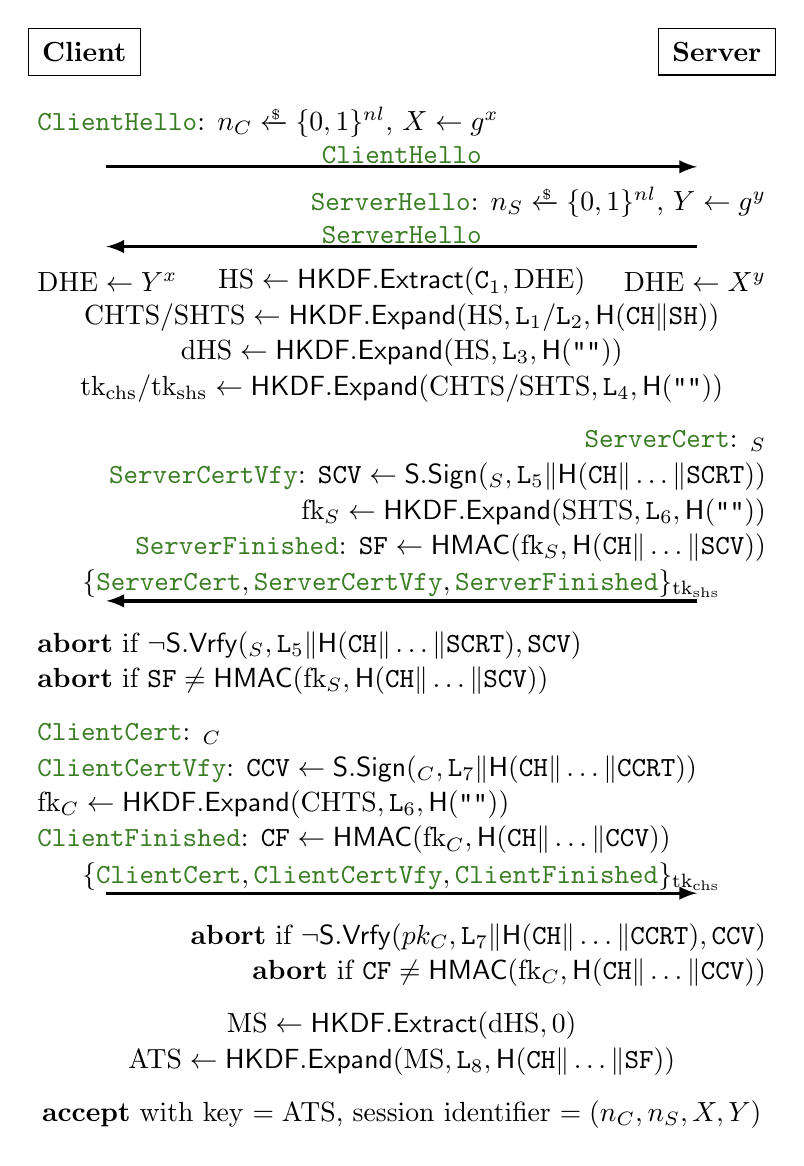
\begin{tikzpicture}
	% Set the X coordinates of the client, server, and arrows
	\edef\ClientX{0}
	\edef\ArrowLeft{0}
	\iffull
	\edef\ArrowRight{12}
	\edef\ServerX{12}
	\else
	\edef\ArrowRight{9.5}
	\edef\ServerX{9.5}
	\fi
	% Set the starting Y coordinate
	\edef\Y{0}

	% Draw header boxes
	\node [rectangle,draw,inner sep=5pt,right] at (\ClientX,\Y) {\textbf{Client}};
	\node [rectangle,draw,inner sep=5pt,left] at (\ServerX,\Y) {\textbf{Server}};

	\NextLine[2]
	
	\ClientAction{\TLSmsg{$\CHELO$}: $\nonce_C \sample \{0,1\}^{\nl}$, $X \gets g^x$}
% 	\NextLine
% 	\ClientAction{\TLSmsg{+~$\CKEYS$}: $X \gets g^x$}
	
	%%%%%%%%%%%%%%%%%%%%%%%%%%%%%%%%%%%%%%%%%%%
% 	\NextLine
% 	\SharedAction{$\ES \gets \HKDF.\Extract(0, 0)$}
% 	\NextLine
% 	\SharedAction{$\dES \gets \HKDF.\Expand(\ES, \inputlabel[3], \Hash(\texttt{""}))$}
	%%% we simplify this into a constant
	
	%%%%%%%%%%%%%%%%%%%%%%%%%%%%%%%%%%%%%%%%%%%%%%%%%%%%%%%%%%%%%%%%%%%%%%%%%%%%%%%%%%%%%%%%%%%%%%%%%%%%%%%
	\NextLine[0.75]
	\ClientToServer{\TLSmsg{$\CHELO$}}{}%, \TLSmsg{$\CKEYS$}}{}
	\NextLine[0.75]
	%%%%%%%%%%%%%%%%%%%%%%%%%%%%%%%%%%%%%%%%%%%%%%%%%%%%%%%%%%%%%%%%%%%%%%%%%%%%%%%%%%%%%%%%%%%%%%%%%%%%%%%
	
	\ServerAction{\TLSmsg{$\SHELO$}: $\nonce_S \sample \{0,1\}^{\nl}$, $Y \gets g^y$}
% 	\NextLine
% 	\ServerAction{\TLSmsg{+~$\SKEYS$}: $Y \gets g^y$}
	
	%%%%%%%%%%%%%%%%%%%%%%%%%%%%%%%%%%%%%%%%%%%%%%%%%%%%%%%%%%%%%%%%%%%%%%%%%%%%%%%%%%%%%%%%%%%%%%%%%%%%%%%
	\NextLine[0.75]
	\ServerToClient{\TLSmsg{$\SHELO$}}{}%, \TLSmsg{$\SKEYS$}}{}
	\NextLine[0.75]
	%%%%%%%%%%%%%%%%%%%%%%%%%%%%%%%%%%%%%%%%%%%%%%%%%%%%%%%%%%%%%%%%%%%%%%%%%%%%%%%%%%%%%%%%%%%%%%%%%%%%%%%
	
	\ClientAction{$\DHE \gets Y^x$}
	\ServerAction{$\DHE \gets X^y$}
% 	\NextLine
	\SharedAction{$\HS \gets \HKDF.\Extract(\constant[1], \DHE)$}
	\NextLine
	
% 	\SharedAction{$\CHTS \gets \HKDF.\Expand(\HS, \inputlabel[1], \Hash(\sCHELO \conc \sSHELO))$}
% 	\NextLine
% 	\SharedAction{$\SHTS \gets \HKDF.\Expand(\HS, \inputlabel[2], \Hash(\sCHELO \conc \sSHELO))$}
% 	\NextLine
	\SharedAction{$\CHTS/\SHTS \gets \HKDF.\Expand(\HS, \inputlabel[1]/\inputlabel[2], \Hash(\sCHELO \conc \sSHELO))$}
	\NextLine
	\SharedAction{$\dHS \gets \HKDF.\Expand(\HS, \inputlabel[3], \Hash(\texttt{""}))$}
	\NextLine
	
% 	\SharedAction{$\tkchs \gets \HKDF.\Expand(\CHTS, \inputlabel[4], \Hash(\texttt{""}))$}
% 	\NextLine
% 	\SharedAction{$\tkshs \gets \HKDF.\Expand(\SHTS, \inputlabel[4], \Hash(\texttt{""}))$}
	\SharedAction{$\tkchs/\tkshs \gets \HKDF.\Expand(\CHTS/\SHTS, \inputlabel[4], \Hash(\texttt{""}))$}
	\NextLine[0.5]
	
	%\NextLine
	%\SharedAction{$\tkchs, iv_{chs} \gets \HKDF.\kExp(\CHTS, \inputlabel[n], H_n)$}
	%\NextLine
	%\SharedAction{$\tkshs, iv_{shs} \gets \HKDF.\kExp(\SHTS, \inputlabel[n], H_n)$}
	%%%%%%%%%%%%%%%%%%%%%%%%%%%%%%%%%%%%%%%


% 	\NextLine
% 	\ServerAction{\TLSmsg{$\{\ENCEX\}$}: $\vec{ext}_S$}
% 	\NextLine
% 	\ServerAction{\TLSmsg{$\{\CERTR\}^*$}: $\inputlabel[n]$}
	\NextLine
	\ServerAction{\TLSmsg{$\mSCERT$}: $\pk_S$}
	\NextLine
	\ServerAction{\TLSmsg{$\mSCERTV$}: $\sSCERTV\gets\SIGScheme.\SIGSign(\sk_S, \inputlabel[5] \conc \Hash(\sCHELO \conc \ldots \conc \sSCERT))$}
	\NextLine
	\ServerAction{$\SFK \gets \HKDF.\Expand(\SHTS, \inputlabel[6],\Hash(\texttt{""}))$}
	\NextLine
	\ServerAction{\TLSmsg{$\SFIN$}: $\sSFIN \gets \HMAC(\SFK, \Hash(\sCHELO \conc \ldots \conc \sSCERTV))$}

	%%%%%%%%%%%%%%%%%%%%%%%%%%%%%%%%%%%%%%%%%%%%%%%%%%%%%%%%%%%%%%%%%%%%%%%%%%%%%%%%%%%%%%%%%%%%%%%%%%%%%%%
	\NextLine
	\ServerToClient{$\{\TLSmsg{\mSCERT}, \TLSmsg{\mSCERTV}, \TLSmsg{\SFIN}\}_{\tkshs}$}{}
	\NextLine
	%%%%%%%%%%%%%%%%%%%%%%%%%%%%%%%%%%%%%%%%%%%%%%%%%%%%%%%%%%%%%%%%%%%%%%%%%%%%%%%%%%%%%%%%%%%%%%%%%%%%%%%
	
	\ClientAction{\textbf{abort} if $\neg \SIGScheme.\SIGVerify(\pk_S, \inputlabel[5] \conc \Hash(\sCHELO \conc \ldots \conc \sSCERT), \sSCERTV)$}
	\NextLine
	\ClientAction{\textbf{abort} if $\sSFIN \neq \HMAC(\SFK, \Hash(\sCHELO \conc \ldots \conc \sSCERTV))$}
	\NextLine[1.5]
	
	%%%%%%%%%%%%%%%%%%%%%%%%%%%%%%%%%
	
% 	\SharedAction{$\MS \gets \HKDF.\Extract(\dHS, 0)$}
% 	\NextLine
	
% 	\AcceptStage{3}{$\CATS \gets \HKDF.\Expand(\MS, \inputlabel[xxx], \Hash(\sCHELO \conc \ldots \conc \sSFIN))$}
% 	%\NextLine
% 	%\SharedAction{$\tkcapp, iv_{capp} \gets \HKDF.\kExp(\CATS, \inputlabel[n], H_n)$}
% 	\NextLine[1.5]
% 	
% 	\AcceptStage{4}{$\SATS \gets \HKDF.\Expand(\MS, \inputlabel[xxx], \Hash(\sCHELO \conc \ldots \conc \sSFIN))$}
% 	%\NextLine
% 	%\SharedAction{$\tksapp, iv_{sapp} \gets \HKDF.\kExp(\SATS, \inputlabel[n], H_n)$}
% 	\NextLine[1.5]
% 	
% 	\AcceptStage{5}{$\EMS \gets \HKDF.\Expand(\MS, \inputlabel[xxx], \Hash(\sCHELO \conc \ldots \conc \sSFIN))$}
% 	\NextLine[1.5]
	
% 	\Encryption[<-,dashed]{record layer, AEAD-encrypted with key $\tksapp$ (optional)}{}
% 	\NextLine[1]
	
	%%%%%%%%%%%%%%%%%%%%%%%%%%%%%%%%%
	
	\ClientAction{\TLSmsg{$\mCCERT$}: $\pk_C$}
	\NextLine
	\ClientAction{\TLSmsg{$\mCCERTV$}: $\sCCERTV \gets \SIGScheme.\SIGSign(\sk_C, \inputlabel[7] \conc \Hash(\sCHELO \conc \ldots \conc \sCCERT))$}
	\NextLine
	\ClientAction{$\CFK \gets \HKDF.\Expand(\CHTS, \inputlabel[6],\Hash(\texttt{""}))$}
	\NextLine
	\ClientAction{\TLSmsg{$\CFIN$}: $\sCFIN \gets \HMAC(\CFK,  \Hash(\sCHELO \conc \ldots \conc \sCCERTV))$}

	%%%%%%%%%%%%%%%%%%%%%%%%%%%%%%%%%%%%%%%%%%%%%%%%%%%%%%%%%%%%%%%%%%%%%%%%%%%%%%%%%%%%%%%%%%%%%%%%%%%%%%%
	\NextLine
	\ClientToServer{$\{\TLSmsg{\mCCERT}, \TLSmsg{\mCCERTV}, \TLSmsg{\CFIN}\}_{\tkchs}$}{}
	\NextLine
	%%%%%%%%%%%%%%%%%%%%%%%%%%%%%%%%%%%%%%%%%%%%%%%%%%%%%%%%%%%%%%%%%%%%%%%%%%%%%%%%%%%%%%%%%%%%%%%%%%%%%%%

	\ServerAction{\textbf{abort} if $\neg \SIGScheme.\SIGVerify(pk_C, \inputlabel[7] \conc \Hash(\sCHELO \conc \ldots \conc \sCCERT), \sCCERTV)$}
	\NextLine
	\ServerAction{\textbf{abort} if $\sCFIN \neq \HMAC(\CFK, \Hash(\sCHELO \conc \ldots \conc \sCCERTV))$}
	\NextLine
	
	
	%% abstract 'application traffic secret' being derived here
	\NextLine[0.5]
	\SharedAction{$\MS \gets \HKDF.\Extract(\dHS, 0)$}
	\NextLine
	\SharedAction{$\ATS \gets \HKDF.\Expand(\MS, \inputlabel[8], \Hash(\sCHELO \conc \ldots \conc \sSFIN))$}
	
% 	\AcceptStage{6}{$\RMS \gets \HKDF.\Expand(\MS, \inputlabel[xxx], \Hash(\sCHELO \conc \ldots \conc \sCFIN))$}
% 	\NextLine[1.5]
	
% 	\Encryption[->,dashed]{record layer, AEAD-encrypted using key $\tkcapp$}{}
% 	\NextLine[1]
% 	\Encryption[<-,dashed]{record layer, AEAD-encrypted with key $\tksapp$}{}
	
	\NextLine[1.5]
	\SharedAction{\textbf{accept} with key~$\skey = \ATS$, session identifier~$\sid = (\nonce_C, \nonce_S, X, Y)$}
\end{tikzpicture}
}
\end{minipage}

	\hspace{-0.5cm}
	\begin{minipage}[t]{\iffull0.44\else0.35\fi\textwidth}
\iffull\else\resizebox{5cm}{!}{\fi %% resizebox in lncs
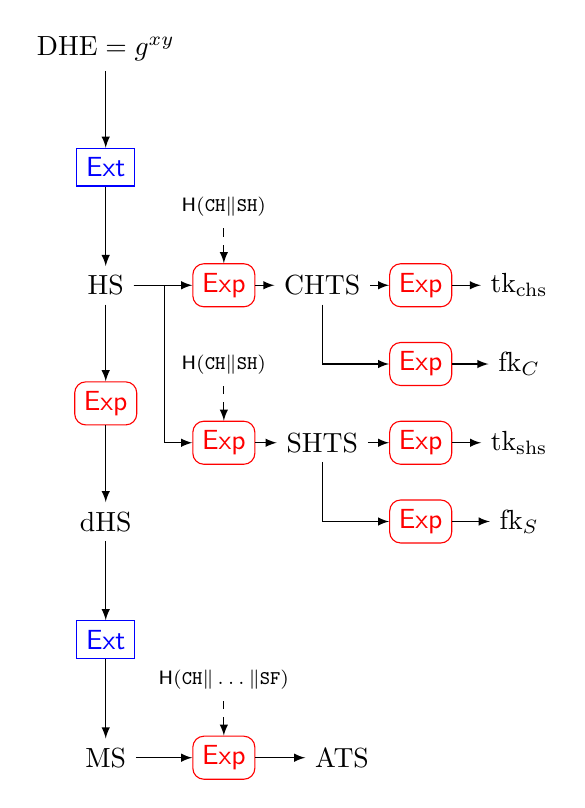
\begin{tikzpicture}[on grid]
	\tikzstyle{extract}=[Blue,draw,rectangle]
	\tikzstyle{expand}=[Red,draw,rectangle,rounded corners]
	\tikzstyle{context}=[latex-,dashed,font=\scriptsize]
	
	%
	% main secrets
	%
	\node (DHE) {$\DHE = g^{xy}$};
	\node [below=3 of DHE] (HS) {$\HS$};
	\node [below=3 of HS] (dHS) {$\dHS$};
	\node [below=3 of dHS] (MS) {$\MS$};
	
	%
	% main secret derivation
	%
	\node [extract,below=1.5 of DHE] (ext-HS) {$\sExtract$};
	\node [expand,below=1.5 of HS] (exp-dHS) {$\sExpand$};
	\node [extract,below=1.5 of dHS] (ext-MS) {$\sExtract$};
	
	\begin{scope}[-latex]
		\draw (DHE) -- (ext-HS);
		\draw (ext-HS) -- (HS);
		\draw (HS) -- (exp-dHS);
		\draw (exp-dHS) -- (dHS);
		\draw (dHS) -- (ext-MS);
		\draw (ext-MS) -- (MS);
	\end{scope}
	
	%
	% CHTS secrets and derivation
	%
	\node [right=2.75 of HS] (CHTS) {$\CHTS$};
	\node [right=2.5 of CHTS] (tkchs) {$\tkchs$};
	\node [below right=1 and 2.5 of CHTS] (CFK) {$\CFK$};
	
	\node [expand,right=1.5 of HS] (exp-CHTS) {$\sExpand$};
	\draw [context] (exp-CHTS) -- ++(0,0.75) node [above] {$\Hash(\sCHELO \conc \sSHELO)$};
	
	\node [expand,right=1.25 of CHTS] (exp-tkchs) {$\sExpand$};
	\node [expand,below right=1 and 1.25 of CHTS] (exp-CFK) {$\sExpand$};
	
	\begin{scope}[-latex]
		\draw (HS) -- (exp-CHTS);
		\draw (exp-CHTS) -- (CHTS);
		\draw (CHTS) -- (exp-tkchs);
		\draw (exp-tkchs) -- (tkchs);
		\draw (CHTS) |- (exp-CFK);
		\draw (exp-CFK) -- (CFK);
	\end{scope}
	
	%
	% SHTS secrets and derivation
	%
	\node [below right=2 and 2.75 of HS] (SHTS) {$\SHTS$};
	\node [right=2.5 of SHTS] (tkshs) {$\tkshs$};
	\node [below right=1 and 2.5 of SHTS] (SFK) {$\SFK$};
	
	\node [expand,below right=2 and 1.5 of HS] (exp-SHTS) {$\sExpand$};
	\draw [context] (exp-SHTS) -- ++(0,0.75) node [above] {$\Hash(\sCHELO \conc \sSHELO)$};
	
	\node [expand,right=1.25 of SHTS] (exp-tkshs) {$\sExpand$};
	\node [expand,below right=1 and 1.25 of SHTS] (exp-SFK) {$\sExpand$};
	
	\begin{scope}[-latex]
		\draw (HS) -- ++(0.75,0) |- (exp-SHTS);
		\draw (exp-SHTS) -- (SHTS);
		\draw (SHTS) -- (exp-tkshs);
		\draw (exp-tkshs) -- (tkshs);
		\draw (SHTS) |- (exp-SFK);
		\draw (exp-SFK) -- (SFK);
	\end{scope}
	
	%
	% ATS secret and derivation
	%
	\node [right=3 of MS] (ATS) {$\ATS$};
	
	\node [expand,right=1.5 of MS] (exp-ATS) {$\sExpand$};
	\draw [context] (exp-ATS) -- ++(0,0.75) node [above] {$\Hash(\sCHELO \conc \dots \conc \sSFIN)$};
	
	\begin{scope}[-latex]
		\draw (MS) -- (exp-ATS);
		\draw (exp-ATS) -- (ATS);
	\end{scope}
	
\end{tikzpicture}
\iffull\else}\fi %% resizebox in lncs
\end{minipage}

	
	%
	% Legend
	%
	\begin{minipage}{0.95\textwidth}
	\vspace{0.25cm}%
	\scriptsize%
	\begin{tabular}{lllll}
		\multicolumn{2}{l}{\textbf{Protocol flow legend}}
			&~~~& \multicolumn{2}{l}{\textbf{Message Abbreviations}} \\
		{\TLSmsg{$\mathtt{MSG}$}:~$Z$}	& message $\mathtt{MSG}$ sent, containing $Z$
			&& \TLSmsg{$\sCHELO$}	& \TLSmsg{$\CHELO$} \\
		$\{\TLSmsg{\mathtt{MSG}}\}_K$	& message AEAD-encrypted with~$K = \tkshs / \tkchs$
			&& \TLSmsg{$\sSHELO$}	& \TLSmsg{$\SHELO$} \\
			&&& \TLSmsg{$\sCCERT/\sSCERT$}~	& \TLSmsg{$\mathtt{Client/}\mSCERT$} \\
			&&& \TLSmsg{$\sCCERTV/\sSCERTV$}	& \TLSmsg{$\mathtt{Client/}\mSCERTV$} \\
			&&& \TLSmsg{$\sCFIN/\sSFIN$}	& \TLSmsg{$\mathtt{Client/}\SFIN$} \\
	\end{tabular}
% 	\begin{tabular}{ll}
% 		\TLSmsg{+~$\mathtt{MSG}$}	& message sent as extension within previous message \\
% 		\TLSmsg{$\mathtt{MSG}^*$}	& message only sent for intended client authentication \\
% 	\end{tabular}
	\end{minipage}
	
	\caption{%
		The simplified TLS~1.3 main Diffie--Hellman handshake protocol (left) and key schedule (right).
		Values~$\inputlabel[i]$ and~$\constant[i]$ indicate bitstring labels, resp.\ constant values, (distinct per~$i$).
		Boxes $\sExtract$ and $\sExpand$ denote $\HKDF$ extraction resp.\ expansion, dashed inputs to~$\sExpand$ indicating context information (see protocol figure for detailed computations).
	}
	\label{fig:tls-protocol}
\end{figure}

In the TLS~1.3 handshake, the client acts as initiator and the server as responder.
Within $\HELO$ messages, both send nonce values~$\nonce_C$ resp.\ $\nonce_S$ together with ephemeral Diffie--Hellman shares~$g^x$ resp.\ $g^y$.
Based on these values, both parties extract a handshake secret~$\HS$ from the shared DH value~$\DHE = g^{xy}$ using $\HKDF.\Extract$ with a constant salt input.%
\fullelse{\footnote{This salt input becomes relevant for pre-shared key handshakes, but in the full handshake takes the constant value~$\constant[1] = \Expand(\Extract(0,0), \texttt{"derived"}, \Hash(\texttt{""}))$.}}{ }
In a second step, client and server derive their respective handshake traffic keys~$\tkchs$, $\tkshs$ and MAC keys~$\CFK$, $\SFK$ through two levels of $\HKDF.\Expand$ steps from the handshake secret~$\HS$, including in the first level distinct labels and the hashed communication transcript~$\Hash(\sCHELO \conc \sSHELO)$ so far as context information.

The handshake traffic keys are then used to encrypt the remaining handshake messages.
First the server, then the client send their certificate (carrying their identity and public key), a signature over the hashed transcript up to including their certificate\fullonly{ ($\Hash(\sCHELO \conc \dots \conc \sSCERT)$, resp.\ $\Hash(\sCHELO \conc \dots \conc \sCCERT)$)}, as well as a MAC over the (hashed) transcript up to incl.\ their signatures\fullonly{ ($\Hash(\sCHELO \conc \dots \conc \sSCERTV)$, resp.\ $\Hash(\sCHELO \conc \dots \conc \sCCERTV)$)}.
Note the similarity to \SIGMAI here:
each party signs both nonces and DH values (within $\sCHELO \conc \sSHELO$, modulo transcript hashing) together with a unique label,
and then MACs both nonces and their own identity (the latter being part of their certificate).%
\fullelse{\footnote{Instead of using distinct labels for the client and server MAC computations, TLS~1.3 employs distinct MAC keys for client and server, achieving separation between the two MAC values this way.}}{ }
The application traffic secret~$\ATS$---which we treat as the session key~$\skey$, unifying secrets of both client and server---is then derived from the master secret~$\MS$ through $\HKDF.\Expand$ with handshake context up to the $\SFIN$ message.
The master secret in turn is derived through (context-less) $\Expand$ and $\Extract$ from the handshake secret~$\HS$.


\iffull
\subsection{Handling the TLS~1.3 Key Schedule}
\else
\subsubsection*{Handling the TLS~1.3 key schedule\lncsdot}
\fi

\iffull
As mentioned before, the message flow of the TLS~1.3 handshake relatively closely follows the \SIGMAI design~\cite{C:Krawczyk03,SIGMA-fullversion} (cf.\ Figure~\ref{fig:sigma-protocol}):
after exchanging nonces and DH shares (in $\HELO$) from both sides, the remaining (encrypted) messages carry identities ($\CERT$), signatures over the nonces and DH shares ($\CERTV$), and MACs over the nonces and identities ($\FIN$).

What crucially differentiates the TLS~1.3 handshake from the basic \SIGMAI design (beyond putting more under the respective signatures and MACs, which does not negatively affect the key exchange security we are after) is the way keys are derived.
While \SIGMAI immediately derives a master key through a random oracle with input \emph{both} the shared DH secret \emph{and} the session identifying nonces and DH shares,
TLS~1.3 separates them in its HKDF-based extract-then-expand key schedule:
The core secrets---handshake secret ($\HS$) and master secret ($\MS$)---are derived without further context purely from the shared DH secret~$\DHE = g^{xy}$ (beyond other constant inputs).
Only when deriving the specific-purpose secrets---handshake traffic keys ($\tkchs$, $\tkshs$), MAC keys ($\CFK$, $\SFK$), and session key ($\ATS$)---is context added to the key derivation, including in particular the nonces and DH shares identifying the session.
To complicate matters even further, this context is hashed before entering key derivation (or signature and MAC computation), and the final session key~$\ATS$ depends on more messages than just the session-identifying ones.
Since our tighter security proof for the SIGMA(-I) protocol (cf.\ Section~\ref{sec:sigma-proof}) heavily makes use of (exactly) the session identifiers being input together with DH secrets to a random oracle when programming the latter,
the question arises how to treat the TLS~1.3 key schedule when aiming at a similar proof strategy.

In their concurrent work, Diemert and Jager~\cite{JC:DieJag20} satisfy this requirement by modeling the full derivation of each stage key in their multi-stage treatment as a separate random oracle.
This directly connects inputs to keys, but results in a monolithic random oracle treatment of the key schedule which loses the independence of the intermediate $\HKDF.\Extract$ and $\HKDF.\Expand$ steps in translation.

We overcome the technical obstacle of this linking while staying closer to the structure of TLS~1.3's key schedule.
First of all, we directly model both $\HKDF.\Extract$ and $\HKDF.\Expand$ as individual (programmable) random oracles,
which leads to a slightly less excessive use of the random oracle technique.
We then have to carefully orchestrate the programming of intermediate secrets and session keys in a two-level approach,
connecting them through constant-time look-ups,
and taking into account that inputs to deriving the session keys depend on values established through the intermediate secrets (namely, the server's $\FIN$ MAC).
Along the way, we separately ensure that we recognize any hashed inputs of interest that the adversary might query to the random oracle, without modeling the hash function~$\Hash$ as a random oracle itself.
By tracking intermediate programming points (especially $\HS$ and~$\MS$) in the random oracles, we recover the needed capability of linking sessions and their session identifiers and DH shares exchanged to the corresponding session keys.
This finally allows us to again (efficiently) determine when and on what input to query the strong Diffie--Hellman oracle when programming challenge DH shares into the TLS~1.3 key exchange execution during the proof.

\else

What crucially differentiates the TLS~1.3 handshake from the basic \SIGMAI design is the way keys are derived.
While \SIGMAI derives its master key through a random oracle with input \emph{both} the shared DH secret \emph{and} the session identifying nonces and DH shares,
TLS~1.3 separates them in its HKDF-based extract-then-expand key schedule:
The core $\HS$ and $\MS$ secrets are derived \emph{without} further context purely from the shared DH secret~$\DHE = g^{xy}$.
Only when deriving the specific-purpose secrets---handshake traffic keys, MAC keys, and the session key~$\ATS$---are the nonces and DH shares add as session-identifying context.
To complicate matters even further, this context is hashed and the final session key~$\ATS$ depends on more messages than just the session-identifying ones.
Recall that the original techniques by Cohn-Gordon et al.~\cite{C:CCGJJ19} heavily relies on (exactly) the session identifiers being input together with DH secrets to a random oracle when programming the latter,
impeding a more direct application like for \SIGMAI.
In their concurrent work, Diemert and Jager~\cite{JC:DieJag20} satisfy this requirement by modeling the full derivation of each stage key in their multi-stage treatment as a separate random oracle.
This directly connects inputs to keys, but results in a monolithic random oracle treatment of the key schedule which loses the independence of the intermediate $\HKDF.\Extract$ and $\HKDF.\Expand$ steps in translation.
As we will show next, we overcome the technical obstacle of this linking while directly modeling $\HKDF.\Extract$ and $\HKDF.\Expand$ as individual random oracles,
carefully orchestrating the programming of intermediate secrets and session keys and connecting them through constant-time look-ups.
This leads to a slightly less excessive use of the random oracle technique and allows us to stay much closer to the structure of TLS~1.3's key schedule.

\fi


% \hrulefill
%
%\subsection*{\color{Red}Problems with the TLS key schedule compared to SIGMA}
%
%\begin{itemize}
%	\item Proof strategy needs $(n_C, n_S, g^x, g^y, g^{xy})$ in the RO query to (efficiently!) do StrongDH look-ups.
%	\item In TLS, we have $HS \gets Extract(0, g^{xy})$ which doesn't allow for this; the handshake transcript (ClientHello+ServerHello), which include $(n_C, g^x)$ resp.\ $(n_S, g^y)$ only enter key derivations in Expand calls.
%	\item This captures the derivation of $tk_{hs}$ ($k_e$ in \SIGMAI notation) and the MAC keys ($k_t$ in SIGMA), but not the expansion of~$dHS$ towards the master secret is \emph{without} transcript.
%	\item However, the final session key $tk_{app}$ ($k_s$ in SIGMA) will be derived from $MS$ \emph{with} transcript.
%\end{itemize}
%
%
%\subsection*{\color{Red}Updated proof Idea}
%
%\begin{itemize}
%	\item We will have two random oracles:
%	\begin{enumerate}
%		\item $RO_1 = \Extract$ will map $\DHE$ values to $\HS$ (and later derived $\dHS$ to $\MS$), we keep (two) tables mapping $\HS$ and $\MS$ values back to~$\DHE$ ($Q1[\HS] = \DHE$, resp.\ $Q2[\MS] = \DHE$), so that we know which $\DHE$ inputs to $\Expand$ originated from.
%		
%		\item $RO_2 = \Expand$ will capture expansion from $\HS$ and $\MS$. Here is where context information ($g^x, g^y$ through $\CHELO$, $\SHELO$ message inputs) enters the key derivation.
%	\end{enumerate}
%	
%	\item Comparing with SIGMA, we treat HS as the master key. While this is not derived from sid, we can figure out what sid it belongs to because immediately afterwards it is used within Expand together with the sid.
%	
%% 	\item $MS \gets Extract(dHS, 0)$ is computed regularly from $dHS = RO_1(Z, ...)$ (and we immediately do this when a $dHS$ call in $RO_1$ happens), but we will store the intermediary mapping of values $Z$ to $MS$ as $Q[MS] = Z$. (Read as: $MS$ was derived from $Z$ in $RO_1$.)
%	
%	\item Note: $\Hash$ is \emph{not} a random oracle (but just collision resistant). In order to map hash inputs to $RO_2$ back to the session identifiers, we keep tables mapping all hashed transcripts, $H_i = \Hash(\sCHELO \conc \dots)$, of sessions to their inputs (or at least to the nonces and $g^x, g^y$), so we know when some $H_i$ is used for which we need to lookup the DH share inputs, and the sid it corresponds to.
%	
%	\item When the adversary calls $RO_2(X,  l)$ for some $l$ containing (the hash of) $g^x, g^y$, we can detect if we've seen $X$ (as key to $Q1$/$Q2$) being derived before, and then can call our StrongDH oracle on $(g^x, g^y, Q[X])$.
%	
%	\item Adversary asking~$RO_2$ on some $X$ that results from an encoded challenge \emph{before} the challenge is encoded---bound by probability of $|RO_1|$, but also: isn't it still fine if we detect this later and call our StrongDH oracle then? \fg{Probably not, later detecting means an adversary might have been able to detect this already?}
%	
%	\item Probability that $X$ of any $RO_2$ is later hit by a $RO_1$ output should be birthday-bounded by \#queries to $RO_1$ squared / $|RO_1|$.
%\end{itemize}
%
%
%

\section{Tighter Security Proof for the TLS~1.3 Handshake}
\label{sec:tls-proof}

We now give our second main result, the tighter-security bound \fullelse{for the TLS~1.3 handshake protocol}{for TLS~1.3}.

\begin{theorem}
	\label{thm:tls}
	Let $\advA$ be a key exchange security adversary against the TLS~1.3 handshake protocol as specified in Figure~\ref{fig:tls-protocol} based on a hash function~$\Hash$, a signature scheme~$\SIGScheme$, and a group~$\group$ of prime order~$p$,
	and let the $\HKDF$ functions~$\Extract$ and $\Expand$ in the protocol be modeled as (independent) random oracles~$\RO_1$, resp.~$\RO_2$. 
	For any $(t, \qNewUser, \qSend, \qRevSessionKey, \qRevLongTermKey, \qTest)$-$\KESEC$-adversary against \SIGMAI making at most $\qRO$ queries to the random oracle,
	we give algorithms~$\advB_1$, $\advB_2$, $\advB_3$, and $\advB_4$ in the proof,
	with running times~$t_{\advB_i} \approx t$ (for $i = 1,3,4$) and $t_{\advB_2} \approx t + 2\qRO \log_2 p$ close to that of $\advA$, such that
	\begin{collectinmacro}{\TLSBound}{}{} %%% ===== COLLECT BEGIN =====
	\begin{align*}
		\Adv&^{\KESEC}_{\mTLS}(t, \qNewUser,\qSend, \qRevSessionKey,\qRevLongTermKey,\qTest)
			\leq
% 			\frac{\qSend^2}{2^{\nl}} + \frac{\qSend^2}{2p} + \frac{\qSend^2}{2^{\nl}\cdot p} % sid collisions -- old game hops
			\frac{3\qSend^2}{2^{\nl+1}\cdot p} % sid collisions
			+ \Adv^{\COLL}_{\Hash}(t_{\advB_1})\\ % hash collisions
			&+  2 \cdot \Adv^{\strongDH}_{\group}(t_{\advB_2},\qRO)
			+\frac{\qRO\cdot \qSend}{2^{\kl-1}}
			+ \Adv^{\muEUFCMA}_{\SIGScheme}(t_{\advB_3},\qNewUser,\qSend,\qSend,\qRevLongTermKey)\\
			&+ \Adv^{\muEUFCMA}_{\HMAC}(t_{\advB_4}, \qSend,\qSend,1, \qSend,1,0).
	\end{align*}
	\end{collectinmacro}
	\TLSBound
	Here,
	$\nl = 256$ is the nonce length in TLS~1.3,
	$\kl$ is the output length of~$\RO_2 = \HKDF.\Expand$,
	$\group$ is the used Diffie--Hellman group of prime order~$p$,
	and $\qSend \cdot \qRO \leq 2^{\kl-3}$.%
	\footnote{We simplify the factor on $\Adv^{\strongDH}_{\group}$ to~$2$ by assuming $\qSend \cdot \qRO \leq 2^{\kl-3}$, which is true for any reasonable real-world parameters.
	See the proof for the exact bound.}
\end{theorem}

\iffull
\else

%%%%%%%%%%%%%%%%%%%%%%%%%%%%%%%%%%%%%%%%%%%%%%%%%%%%%%%%%%%%%%%%%%%%%%%%%%%%%%%%%%%%%%%%%%%%%%%%
%% TLS Proof VERY short version for lncs / non-full
%%%%%%%%%%%%%%%%%%%%%%%%%%%%%%%%%%%%%%%%%%%%%%%%%%%%%%%%%%%%%%%%%%%%%%%%%%%%%%%%%%%%%%%%%%%%%%%%

% \begin{proof}[Proof outline]
\subsubsection*{Proof idea\lncsdot}
Let us first outline the core and novel technical steps, before we give some more proof details below;
for space reasons we defer the full proof to the full version~\cite{EPRINT:DavGun20}.
We note that as all keys in the \SIGMA exchange are derived from the master key $mk$, which is itself derived from the shared Diffie--Hellman secret, all intermediate keys in TLS~1.3 are derived from the handshake secret $\HS$, which is derived directly from the shared Diffie--Hellman secret $\DHE$.
Embedding a DH challenge into all sessions robs the reduction of the ability to compute $\HS$;
as in the \SIGMA proof, we will need to use the strong DH oracle to detect and program queries that would output an inconsistent value of $\HS$.
Since $\HS$ is derived without context, a naive method would have to check every input to $\HKDF.\Extract$ against the DH shares received by each session, which would however result in a non-tight, quadratic runtime loss. 

We instead leverage that the handshake secret~$\HS$ is an internal value, not exposed by any oracle.
The adversary hence cannot detect an inconsistent $\HS$ value until it makes the entire chain of queries leading to one of the keys $\tkshs$, $\tkchs$, $\CFK$, $\SFK$, or $\ATS$ used in $\Send$, $\RevSessionKey$, and $\Test$ responses.
Our reduction prudently sets up a separate bidirectional lookup table for each ``link'' in that chain.
The adversary can make the RO queries in the chain in any order; we need only program the last one for consistency, at which time we have seen the session's DH secret, nonces, and group elements as query inputs.
Linking the output of one key-derivation step to the input of the next this way, the reduction can identify the relevant sessions using only constant time and linear space.
Together with a careful argument that the attacker is unlikely to guess an intermediate chain value, this allows us to treat $\HKDF.\Extract$ and $\HKDF.\Expand$ as two individual random oracles.
Thereby, we stay close to how HKDF is used in TLS~1.3 and obtain two compact strong-DH bounds.
%
% One subtlety that is unique to our proof is that the reduction to the strong DH problem no longer maintains perfect consistency.
% Because key derivation happens as a multi-stage process, it is possible, though unlikely, that the adversary will randomly guess one of the intermediate values of key derivation without making the corresponding RO query.
% If this happens, the reduction does not have a complete ``chain'' and cannot identify which sessions' shared DH secret has been discovered.
% It therefore can neither program the ROs appropriately nor extract the challenge secret from the shared secret, because it does not know which keys are known or which randomness was used by the compromised sessions.
% This flaw leads to a loss of $\frac{2^{kl}}{2^{kl} - \qRO \cdot \qSend}$ in the reduction.
% We assume, as is true for any reasonable choices of the symmetric parameter $kl$, that $\qRO \cdot \qSend \leq 2^{kl -2}$.
% This allows us to upper bound this factor with a much simpler constant.
% \end{proof}

\bigskip

Now we give a more precise view of the structure of our proof, with a particular focus on nonstandard techniques % and the points at which the proof differs from that for \SIGMAI due to aspects unique to TLS~1.3.
and the critical random oracle programming in the reduction step to the strong Diffie--Hellman problem, handling the complexity of TLS~1.3's key schedule.

\begin{proof}
	\let\proofsep\medskip %% tighter spacing in here
	
	\startproof{TLS-short}
	
	We develop the bound via a series of code-based game hops.
	
	\proofngame[initial-game]
	
	The first game $\curGm$ is the key exchange security game (cf.\ Figure~\ref{fig:AKE-security}) for the TLS~1.3 handshake protocol (Figure~\ref{fig:tls-protocol}).
	%, where the formal algorithms~$\KEActivate$ and $\KERun$ execute the steps shown in Figure~\ref{fig:tls-protocol} as well as appropriate maintenance of the session state.
	%
	%execute e capture the two protocol steps for each role in formal algorithms~$\KEActivate$, $\RunRespI$, $\RunInit$, and $\RunRespII$.
	% We briefly define the formal algorithms $\KEActivate$, $\RunRespI$, $\RunInit$, and $\RunRespII$ (following the formal algorithm structure of \SIGMAI from Figure~\ref{fig:sigma-formal}) as follows.
	% Let $\KEActivate$ include all of the client computation up to its first sent message, and $\RunInit$ cover the rest of the client's actions.
	% Let the $\RunRespI$ algorithm perform all of the server's computation up to the generation of its second message,
	% and let the $\RunRespII$ algorithm include all of the server's remaining computation.
	% After acceptance, servers set their peer id to that contained in~$\CCERT$, clients set their peer identity to that in~$\SCERT$, and all sessions set their session key $\skey \gets \ATS$.
	% With these definitions in place,
	So,
	$\Pr[\curGm*\Rightarrow 1] = \Pr[ \Gm^{\KESEC}_{\TLS,\advA} \Rightarrow 1 ]$.
	
	
	\proofngames[collisions]{4}
	
	Over the next four games we ensure the uniqueness of each session's protocol transcript by aborting if an honest session chooses a nonce and DH share that have already been sent or received by another honest session, or if a collision occurs in the hash function $\Hash$. We limit the probability of nonce and DH share collisions using a union bound, and give a simple reduction $\advB_1$ to the collision resistance of the hash function~$\Hash$. We also lazily sample the random oracles $\RO_1$ and $\RO_2$ using internal tables $H_1$ and $H_2$.
	Excluding collisions, we obtain the bound
	$\Pr[\prevGm*\Rightarrow 1] - \Pr[\curGm\Rightarrow 1] \leq \frac{3\qSend^2}{2^{\nl+1}\cdot p}% sid collisions
	+ \Adv^{\COLL}_{\Hash}(t_1)$.
	
	
	\proofngames[copy-keys]{2}
	
	Following the technique of~\cite{C:CCGJJ19}, we let initiator sessions in category~(A) copy session, MAC, and traffic encryption keys from their partners via a table indexed by session IDs. 
	In TLS~1.3, there are two encryption keys $\tkshs$ and $\tkchs$, and two MAC keys $\SFK$ and $\CFK$ to copy. One significant difference from both~\cite{C:CCGJJ19} and our \SIGMAI proof is that the session key $\ATS$ now depends on the messages $\sSCERT$, $\sSCERTV$, and $\sSFIN$. We have not yet ensured that partnered sessions agree on these values. Therefore honest initiators will only copy $\ATS$ from their partners if they received the exact same $(\sSCERT\cab \sSCERTV\cab \sSFIN)$ sent by their partner, which they check via an internal look-up table. Otherwise, $\ATS$ is still computed as in previous games. 
	Since keys are only copied when partners agree on all of the information entering the key derivation function, this change is unobservable to~$\advA$, hence
	$\Pr[\curGm*\Rightarrow 1] = \Pr[\prevGm*\Rightarrow 1]$.
	
	
	\proofngames[programming]{2}
	
	These two games contain both the most critical step and the one that diverges the most from the \SIGMAI proof.
	We let all category~(A) sessions that are not already copying their keys pick the handshake traffic keys $\SHTS$ and $\CHTS$, and the session key $\ATS$ uniformly at random, checking for consistency with the random oracle $\RO_2$ and retroactively programming it when necessary.
	(Category (A) initiator sessions who do not copy $\ATS$ due to tampering sample only $\ATS$.) 
	Then, we eliminate the consistency check and let these sessions' handshake traffic keys and session key be uniformly random and inconsistent with the adversary's queries to $\RO_2$. 
	We argue that the adversary can only detect this inconsistency if it queries $\RO_2$ on the correct input to derive one of $\SHTS$, $\CHTS$, or $\ATS$ for a category~(A) session, an event we refer to as event~$F$. 
	
	We give a reduction $\advB_2$ to the strong DH assumption in group~$\group$ which wins with high probability if event $F$ occurs. 
	Given a challenge $C,D$, algorithm $\advB_2$ simulates Game $7$. It embeds $C$ in the DH shares of all initiators and $D$ in the DH shares of all category~(A) responders. 
	Because $\advB_2$ cannot compute the DH secret for embedded sessions, it uses its $\stDH$ oracle to catch and program all queries to $\RO_2$ which are dependent on this secret. When event~$F$ occurs, $\advB_2$ uses its own randomness to extract the challenge DH secret from the DH secret contained in the query that triggered event~$F$. 
	In addition to the details covered in Section~\ref{sec:tls-proof}, the reduction has a few nuances:
	\begin{enumerate}
		\item If for some category~(A) session, $\advA$ can guess without making the corresponding query any of the intermediate values $\HS = \RO_1(\constant[1],\DHE)$, $\dHS = \RO_2(\HS,\inputlabel[3],\Hash(``"))$, or $\MS = \RO_1(\dHS,0)$, where $\DHE$ is the DH secret associated to some pair of embedded shares $(\X,\Y)$ chosen by honest sessions, then it can trigger event $F$ without ever submitting $\DHE$ to an oracle.
		Without knowing $\DHE$, $\advB_2$ cannot detect this query, so it does not program $\RO_2$ appropriately and the simulation fails.
		$\advB_2$ does not itself compute $\HS$, $\dHS$, or $\MS$ for category~(A) sessions, so if $\advA$ does not make the appropriate queries than all three values are uniformly random and each can be guessed with probability at most~$\frac{\qRO \cdot \qSend}{2^{\kl}}$.  
		
		\item In TLS~1.3, the context string including the Diffie--Hellman shares is hashed with $\Hash$ before it enters the key derivation, so $\advB_2$ cannot directly associate an $\RO_2$ query with an honest~$\sid$.
		We address this by logging hash computations of honest sessions in a reverse look-up table~$R$.
		Then in the $\RO_2$ oracle, $\advB_2$ can use $R$ to efficiently find the context associated with a particular query.
		
	\end{enumerate}
	When $\qRO \cdot \qSend \leq 2^{\kl - 3}$, we obtain the bound
	$\Pr[\prevGm*\Rightarrow 1 ] - \Pr[\curGm*\Rightarrow 1] \leq 2\cdot \Adv^{\strongDH}_{\group}(t_{\advB_2},\qRO) +\frac{\qRO \cdot \qSend}{2^{\kl}}$.
	
	The reduction $\advB_2$ queries the $\stDH$ oracle at most once for each query to $\RO_2$ query and once more when event $F$ occurs.
	Computing the input to each $\stDH$ query requires 1 multiplication and one exponentiation in the base group, which can be done using $1+2\log_2 p$ total group operations. In our runtime analysis, we count each group operation as $1$ step, so $t_{\advB_2} \approx t + 2 \qRO\log_2 p$.
	
	\proofngame[uniform-keys] 
	In game $\curGm$, category~(A) sessions sample all encryption and MAC keys uniformly at random. This is distinguishable only if the adversary can query $\RO$ on a string containing one of the random values $\SHTS$ or $\CHTS$, so by the birthday bound
	$\Pr[\prevGm*\Rightarrow 1 ] - \Pr[\curGm*\Rightarrow 1] \leq \frac{\qRO\cdot \qSend}{2^{\kl}}$.
	
	\proofngames[sigs-and-macs]{4}
	In the remaining games, we eliminate signature and MAC forgeries via straightforward reductions $\advB_3$ and $\advB_4$ to the multi-user EUF-CMA security of $\SIGScheme$ and $\MACScheme$. This gives the bound 
	$
	\Pr[\prevGm*\Rightarrow 1 ] - \Pr[\curGm*\Rightarrow 1] \leq
	\Adv^{\muEUFCMA}_{\SIGScheme}(t_{\advB_3\cab \qNew\cab \qSend\cab \qSend\cab \qRevLongTermKey})
	+ \Adv^{\muEUFCMA}_{\MACScheme}(t_{\advB_4}\cab \qSend\cab \qSend\cab 1\cab \qSend\cab 1\cab 0).
	$
	
	Finally, we argue that $\advA$ has advantage $0$ in game $\curGm$, using logic similar to that in our $\SIGMAI$ proof, with two slight differences: 1. Partnered sessions no longer use labels to distinguish their MAC tags; instead we note that  messages tagged by initiator sessions are strictly longer than messages tagged by responder sessions. 2. We cannot immediately conclude that partnered sessions agree on the same session key because the session key $\ATS$ relies on values that are not contained in the session identifier. However, since we have excluded MAC forgeries, all the information entering the derivation of $\ATS$ is authenticated by the responder session's MAC tag.
\end{proof}

\fi

\iffull
\begin{collectinmacro}{\TLSProofFull}{}{} %%% ===== COLLECT BEGIN =====
\startproof{TLS}
We prove our bound by making an incremental series of changes to the key exchange security game and limiting the amount that each change affects the success probability of $\advA$. 
\newcounter{advB-TLS}

\proofngame[tls-start]

The initial game, Game $\curGm$, is the key exchange security game for TLS played by $\advA$, using the implicit $\KEKGen$, $\KEActivate$, and $\KERun$ routines defined by the TLS protocol specification on the left side of Figure~\ref{fig:tls-protocol}.
(In this game, $\HKDF.\Extract$ and $\HKDF.\Expand$ are modeled by random oracles $\RO_1$ and $\RO_2$ respectively.)
By definition, 
\[\Pr[\curGm\Rightarrow 1] = \Pr[ \Gm^{\KESEC}_{\TLS,\advA} \Rightarrow 1 ].\]

\proofngame[tls-log-nonces]

In game $\prevGm$, we start logging the nonces and group elements chosen by honest sessions. Whenever two honest sessions choose the same nonces or group elements, we set a flag $\bad[C]$. Whenever an honest responder session chooses a nonce and group element that have already been received by another session, we set a flag $\bad[O]$. We also make both random oracles $\RO_1$ and $\RO_2$ lazily sampled using internal tables $H_1$ and $H_2$. These changes only affect the values of the game's internal state, and the view of the adversary remains the same as in $\prevGm$, so 
\[ \Pr[\curGm\Rightarrow 1] = \Pr[\prevGm \Rightarrow 1]. \]

\proofngame[tls-sid-collisions]

Starting with $\curGm$, we abort whenever two honest sessions sample the same nonce or group element and whenever an honest responder samples a nonce and group element that are already in use. Since this happens only after one of the flags $\bad[C]$ and $\bad[O]$ is set, by the identical-until-bad lemma,
\[\Pr[\prevGm*\Rightarrow 1] - \Pr[\curGm*\Rightarrow 1] \leq \Pr[\bad[C] \gets \true\text{ or }\bad[O]\gets \true \text{ in }\prevGm].\]
One nonce and one group element is chosen in each $\RunInitI$ call and each $\RunRespI$ call, so at most one nonce and one group element is chosen for each of the~$\qSend$ queries the adversary makes to its $\Send$ oracle.
We use the birthday bound to limit the probability of a collision (flag $\bad[C]$) in either the set of honest sessions' nonces or the set of honest sessions' DH shares to $\frac{\qSend^2}{2^{\nl+1}\cdot p}$. Every time a responder session chooses a nonce and group element, there are at most $\qSend$ values have already been chosen, so by the union bound $\bad[O]$ is set with probability at most $\frac{\qSend^2}{2^{\nl}\cdot p}$.  Therefore
\[
	\Pr[ \prevGm* \Rightarrow 1] - \Pr[ \curGm* \Rightarrow 1] \leq \frac{3\qSend^2}{2^{\nl+1}\cdot p}.
\]
%%%technically the multiplier could be 3/2, not 2. 
\proofngame[tls-log-sidhashes]

Next, we must ensure that partial transcripts between honest sessions do not collide under the hash function $\Hash$. This is a step unique to the $\TLS$ proof, which hashes all of its context with a collision-resistant hash function before it is input into key-derivation. In $\curGm$, honest sessions will log all of their hash outputs in a look-up table $T$: whenever an honest session computes $d = \Hash(s)$ for some string $s$, it sets $T[d] \gets s$ if $T[d]$ has not already been defined.
If $T[d]$ is not empty, then some prior honest session has computed $d = \Hash(s')$ for some string $s'$. The session will set a flag $\bad[\Hash]$ if $s' \neq s$, noting that a collision has occurred. We also remove the now superfluous $\bad[C]$ flag. These administrative changes do not affect the view of the adversary, so 
\[\Pr[\curGm*\Rightarrow 1 ] = \Pr[\prevGm* \Rightarrow 1]. \]

\proofngame[tls-hash-collisions]

\stepcounter{advB-TLS}
In Game $\curGm$, we abort whenever hashes computed by honest sessions collide (i.e. the $\bad[\Hash]$ flag is set). By the identical-until-bad lemma,
\[ \Pr[\prevGm \Rightarrow 1] - \Pr[\curGm\Rightarrow 1] \leq \Pr[\bad[\Hash] \gets \true\text{ in }\prevGm].\]
We bound the probability that $\bad[\Hash]$ is set via a reduction $\curadvB$ to the collision-resistance security of $\Hash$. 
The reduction simulates $\prevGm$ honestly for the adversary $\advA$. 
If the flag $\bad[\Hash]$ is set, then the reduction has obtained strings $s$, $s'$, and $d$ such that $s' \neq s$, and $\Hash(s) = \Hash(s') = d$. Then $\curadvB$ outputs $(s,s')$ and wins the collision-resistance game, so $\genAdv{cr}{\Hash}{\curadvB} \geq \Pr[\bad[\Hash] \gets \true\text{ in } \prevGm].$
The runtime~$t_{\curadvB}$ of $\curadvB$ approximately equals the runtime of $\advA$ in $\prevGm$.
It follows that 
\[ \Pr[\prevGm* \Rightarrow 1] - \Pr[\curGm* \Rightarrow 1] \leq \Adv^{\COLL}_{\Hash}(t_{\curadvB}).\]

\proofngame[tls-log-keys]

In Game $\curGm$, we remove the superfluous $\bad[\Hash]$ flag and make additional internal changes to the behavior of honest sessions. 
As in the \SIGMAI proof, all honest initatior sessions now log the first message they send in a set $\Sent$, and honest responder sessions use this set to check whether their first received message came from an honest session without tampering. If so, we say the responder session has an ``honest origin partner."
In the \SIGMAI protocol, partnering between honest sessions was sufficient to ensure agreement on the derived master key and all subsequently computed keys, since partners are guaranteed to hold the same nonces and group elements. 
In TLS~1.3, partnering also ensures agreement on the handshake traffic secrets $\SHTS$ and $\CHTS$, but it does not ensure agreement on the session key $\ATS$. 
Therefore the responder only logs the handshake traffic keys $\SFK, \CFK, \tkshs,$ and $\tkchs$ in a look-up table $\S$ under its session identifier. 
In addition to the session identifier, the application traffic secret $\ATS$ depends on the server's identity $\sSCERT$, signature $\sSCERTV$, and MAC tag $\sSFIN$. 
These values are not necessarily shared by partner sessions in Game $\curGm$, so two partnered sessions may derive different values of $\ATS$.   
The responder session therefore logs its session key $\ATS$ in a second look-up table $\S'$ indexed by all of the dependencies of the session key: $\sid, \sSCERT,\sSCERTV$, and $\sSFIN$. 
All of this is just bookkeeping, so 
\[ \Pr[\curGm*\Rightarrow 1] = \Pr[\prevGm* \Rightarrow1].\]

\proofngame[tls-copy-keys]

Going forward from Game $\curGm$, honest initiators copy their key material from tables $\S$ and $\S'$ if it is consistent for them to do so.
In the case where the adversary has tampered with the values of $\sSCERT$, $\sSCERTV$, or $\sSFIN$, the partner's session key depends on the untampered values and should not be copied.
Therefore honest initiators always copy encryption and MAC keys from the table $\S$ if they have an honest partner session, but they only copy $\ATS$ when the $\sSCERT, \sSCERTV$, and $\sSFIN$ messages they received match the ones sent by their partner.
The initiator session can check whether tampering occurred using the table $\S'$, which will contain a session key $\ATS$ at index $\sid \conc \sSCERT \conc \sSCERTV \conc \sSFIN$ if and only if the honest partner session computed and sent $\sSCERT$, $\sSCERTV$, and $\sSFIN$.

We argue that all copied keys are consistent with the keys that would be derived in $\prevGm$.
Recall that partnered sessions agree on the nonces and the DH shares $\X$ and $\Y$ as components of $\sid$, so they also agree on the shared DH secret $\Zz$ associated with the pair $(\X,\Y)$. 
Partnered sessions therefore agree on the handshake secret $\HS$, which is derived from $\Zz$ without context, and on the handshake traffic secrets, which are derived with the session identifier as context.
Thus partnered sessions agree on the values of the handshake traffic keys $\SFK,\CFK,\tkshs$, and $\tkchs$ which are derived from the handshake traffic secrets. 
For the adversary it is hence unobservable if honest sessions compute the handshake traffic keys themselves, or copy the keys from their partners.
By agreeing on the handshake secret $\HS$, partnered sessions will also agree on the master secret $\MS$, which is derived from $\HS$ without context. 
The if $\sSCERT$, $\sSCERTV$, and $\sSFIN$ are left untampered, both sessions will derive the session key as $\RO_2(\MS, \inputlabel[8],\Hash(\sid \conc \sSCERT \conc \sSCERTV \conc \sSFIN)])$. Hence it is again unobservable whether an honest initiator derives $\ATS$ itself or copies $\ATS$ from an honest partner which agrees on the values of $\sSCERT$, $\sSCERTV,\sSFIN$; consequently
\[ \Pr[\curGm* \Rightarrow 1] = \Pr[\prevGm* \Rightarrow 1].\]

%\proofngame[tls-log-guessing]
%While the \SIGMAI protocol uses only one random oracle to derive its master key, the TLS protocol's key schedule uses both $\HKDF.\Extract$ and $\HKDF.\Expand$ multiple times to obtain the final keys. We therefore need to ensure that the adversary $\advA$ is not able to guess intermediate values in the key derivation process without making the corresponding queries to $\RO_1$ and $\RO_2$. To this end, in game $\curGm$ we make random oracle $\RO_2$ log the first input $s$ of each query in a list $W$. Whenever $\RO_1$ or $\RO_2$ samples a response to a new query (including both adversarial queries and queries made by the game), they set a flag $\bad[W]$ if the response was the input to a prior $\RO_2$ query, using the list $W$ to efficiently check the condition. This is again just bookkeeping, so 
%\[ \Pr[\curGm* \Rightarrow 1] = \Pr[\prevGm* \Rightarrow 1].\]

%\proofngame[tls-no-guessing]
%We now eliminate the possibility of guessing the intermediate values of key derivation. In Game $\curGm$, the game aborts when an $\RO_1$ or $\RO_2$ would return a value the adversary has already queried to $\RO_2$ (i.e., when the $\bad[W]$ flag is set). By the identical-until bad lemma,
%\[ \Pr[\prevGm \Rightarrow 1] - \Pr[\curGm\Rightarrow 1] \leq \Pr[\bad[W] \gets \true\text{ in } \prevGm].\]
%We bound the right-hand side of this equation.  Let $hl_1$ be the output length of $\RO_1$, and let $hl_2$ be the output length of $\RO_2$. Since the responses to random oracle queries are sampled randomly, they are independent of the contents of the list $W$ of prior inputs to $\RO_2$.
% Each $\RunInit$ or $\RunRespI$ call queries $\RO_2$ on at most $4$ different inputs (these inputs are $\HS, \SHTS, \CHTS$, and $\MS$), so if the adversary makes $\qRO$ total queries to $\RO_1$ and $\RO_2$, and $\qSend$ queries to the $\Send oracle$, then $W$ has at most $\qRO + 4\qSend$ entries. 
%By the birthday bound and the union bound, the probability that one of the responses from $\RO_1$ or $\RO_2$ collides with an element of $W$ is at most$\bad[R]$ is at most $\frac{(\qRO)(\qRO + 4 \qRO \qSend)}{2^{hl_1}}+ \frac{(\qRO)(\qRO + 4 \qRO \qSend)}{2^{hl_2}}$, hence 
%\[ \Pr[\prevGm \Rightarrow 1] - \Pr[\curGm\Rightarrow 1] \leq \frac{(\qRO)(\qRO + 4 \qRO \qSend)}{2^{hl_1}}+ \frac{(\qRO)(\qRO + 4 \qRO \qSend)}{2^{hl_2}} .\]

\proofngame[tls-uniform-keys]

In Game $\curGm$, all responders sample $\ATS$, $\SHTS$ and $\CHTS$ randomly (unless their values have already been fixed by queries to random oracle $\RO_2$ on the corresponding input), then retroactively programs random oracle $\RO_2$ by setting its internal table $H_2$ on the appropriate input.
%They also update the list $W$ to include the inputs $\HS$ and $\MS$. 
Partnered initiator sessions which have not copied $\ATS$ (i.e., those who received tampered $\sSCERT$, $\sSCERTV$, and $\sSFIN$) also sample $\ATS$ randomly and program $\RO_2$ when necessary.
We choose to program $\ATS$, $\SHTS$, and $\CHTS$, as opposed to only $\mk$ in the \SIGMAI proof, because these three keys are derived with context. 
Most importantly, the DH shares $\X$ and $\Y$ indirectly enter the key derivation for these keys, which will be critical for the reduction in the next step.
This simply moves the lazy sampling process from $\RO_2$ to $\RunRespI$ and $\RunInit$ for certain queries, which is unobservable to the adversary; therefore
\[ \Pr[\curGm* \Rightarrow 1] = \Pr[\prevGm* \Rightarrow 1]. \]

\proofngame[tls-stop-programming]

The step between $\prevGm$ and $\curGm$ is most technically involved step of this proof, and it is also the most significantly altered from the corresponding step in the proof of \SIGMAI. 
In $\curGm$, partnered initiators and responder sessions with honest origin partners will stop maintaining the consistency of their keys $\ATS$, $\SHTS$, and $\CHTS$ with the random oracle $\RO_2$. 
Specifically, responders with honest origin partners sample $\ATS$, $\SHTS$, and $\CHTS$ uniformly at random even if $\RO_2$ has already been queried on the string $\HS,\inputlabel,\sidhash$ for the appropriate label and hash, and they do not retroactively program $\RO_2$. Partnered initiator sessions which have not copied $\ATS$ from their partner also sample $\ATS$ uniformly without checking or programming $\RO_2$. 
These keys are therefore completely random, and they will be inconsistent with any random oracle queries made before or after the keys are sampled.

In order to detect this inconsistency, the adversary must make a query to $\RO_2$ that would, in $\prevGm$, return one of the unprogrammed keys.
Which queries are these? 
They are the queries that an honest responder session with honest origin partner would use to derive $\SHTS$, $\CHTS$, and $\ATS$, and the queries that an honest partnered initiator which received a tampered message would use to derive $\ATS$. 
Formally, let $\sid = (\nonce, \nonce',\X,\Y)$ be the session ID held by some honest responder session with honest origin partner, and let $\sSCERT$, $\sSCERTV$, $\sSFIN$ be the identity, signature, and MAC tag sent by this session. 
Let $\DHE$ be the DH secret corresponding to the pair $(\X,\Y)$.
Then the adversary $\advA$ can detect an inconsistency (in derviations of honest responders) in game $\curGm$ if at any point during the game $\advA$ queries $\RO_2$ on one of the tuples
\[
	(\RO_1(\constant[1],\DHE), \inputlabel,\Hash(\sid))
	\qquad \text{or} \qquad
	(\MS,\inputlabel[8],\Hash(\sid\conc \sSCERT \conc \sSCERTV \conc \sSFIN)),
\]
where $\inputlabel \in \{\inputlabel[1], \inputlabel[2]\}$
and where for some $\HS$, $\dHS$, we have that $\HS = \RO_1(\constant[1],\DHE)$, that $\dHS = \RO_2(\HS,\inputlabel[3],\Hash(\texttt{""}))$, and that $\MS = \RO_1(\dHS,0)$.
Otherwise (for derviations of honest initiators), let $\sid$ be the session ID held by an honest partnered initiator session, and let $\sSCERT$, $\sSCERTV$, and $\sSFIN$ be the identity, signature, and MAC tag received by that session.
For initiator sessions that do not copy~$\ATS$, at least one of these values was not sent by the honest partner.
Then the adversary $\advA$ can detect an inconsistency in game $\curGm$ if at any point it queries $\RO_2$ on the tuple
\[
	(\MS,\inputlabel[8],\Hash(\sid\conc \sSCERT \conc \sSCERTV \conc \sSFIN)),
\]
where for some $\HS$, $\dHS$, we have that $\HS = \RO_1(\constant[1],\DHE)$, that $\dHS = \RO_2(\HS\cab \inputlabel[3]\cab \Hash(\texttt{""}))$, and that $\MS = \RO_1(\dHS,0)$.
Let event $F$ denote the event that the adversary $\advA$ makes at least one of the above queries.
If event $F$ does not occur, then $\ATS$, $\SHTS$, and $\CHTS$ are chosen uniformly at random in both $\prevGm$ and $\curGm$, hence
\[\Pr[\prevGm \Rightarrow 1] - \Pr[\curGm]\Rightarrow 1] \leq \Pr[F\text{ occurs in }\prevGm]. \]
\stepcounter{advB-TLS}%
We bound the probability of event $F$ via a reduction $\curadvB$ to the strong Diffie--Hellman assumption in group~$\group$.
The reduction will make no more queries to its $\stDH$ oracle than $\advA$ makes to its $\RO_2$ oracles.

Given its strong DH challenge $(A = g^a, B= g^b)$ and having access to the strong Diffie--Hellman oracle $\stDH_a$, $\curadvB$ simulates $\prevGm$ for an adversary $\advA$ in the following manner: In all honest initiator sessions, $\curadvB$ samples $r$ uniformly at random from $\ZZ_p$ and sets the session's DH share $\X \gets A \cdot g^r$. In all honest responder sessions with honest origin partner, $\curadvB$ samples $r'$ uniformly from $\ZZ_p$ and sets the session's DH share $\Y \gets B \cdot g^{r'}$. Both of these DH shares are still distributed uniformly over $\ZZ_p$ as long as $p$ is prime and $A$ and $B$ are not the identity.  To extract $g^{ab}$ when event $F$ occurs, the reduction $\curadvB$ will follow the same general strategy as the reduction $\advB_1$ in the proof of \SIGMAI, with four major points of divergence. We address these points first, before giving a full description of $\curadvB$.
\begin{enumerate}
	\item Since $\curadvB$ no longer knows $x$ or $y$ such that $\X = g^x$ or $\Y=g^y$, it cannot compute the Diffie--Hellman secret $\DHE$ or the derived handshake secret $\HS$, so it samples $\HS$ randomly for honest responder sessions with honest origin partners and for honest partnered initiator sessions. The adversary can only tell that $\HS$ was not correctly computed if it notices that $\SHTS$, $\CHTS$, or $\dHS$ are derived from an incorrect value of $\HS$. 
	The former two cases require the adversary to make a query that triggers event $F$. In the latter case, $\dHS$ is not revealed to the adversary through any oracle, so the adversary must notice that $\ATS$, which is derived indirectly from $\dHS$ via the master secret, is derived from an incorrect value of $\HS$. This also requires $\advA$ to make a query that triggers event $F$. Therefore, until event $F$ occurs, this change is unobservable to the adversary.
	\item In the TLS protocol, the context string, including the Diffie--Hellman shares $\X$ and $\Y$, is hashed with $\Hash$ before it enters key derivation, so $\curadvB$ cannot directly associate a query to $\RO_2$ with the honest session(s) whose session ID is being used. The reduction addresses this by having each honest responder with honest origin partner and each honest partnered initiator, log the hash of its context in a reverse look-up table $R$.
	(The context does not include the handshake or master secrets.)
	Then in the $\RO_2$ oracle, $\advB_2$ can use $R$ to efficiently check whether the hash $\sidhash$ of a query is used to derive a handshake or application traffic key.
	\item Due to TLS's complex key schedule, no one random oracle query contains both a pair of Diffie--Hellman shares and the DH secret associated with that pair. Instead, $\curadvB$ will augment the $\RO_1$ and $\RO_2$ oracles to log in a reverse look-up table $T$ the DH secret associated with each of the intermediate values $\HS$, $\dHS$, and $\MS$. The DH secret for $\dHS = \RO_2(\HS,\inputlabel[3],\Hash(\texttt{""}))$ simply be copied from $T[\HS]$, and the DH secret for $\MS = \RO_1(\dHS,0)$ will be copied from $T[\dHS]$. For each query to $\RO_2$ with secret $s$, the reduction can efficiently check using $T$ whether $s$ was derived from some DH secret via $\RO_1$. 
	\item The TLS key schedule uses multiple random oracle queries (if we model $\HKDF.\Extract$ and $\HKDF.\Expand$ as random oracles) whereas the \SIGMAI protocol uses only one. If $\advA$ can guess the intermediate value $\HS = \RO_1(\constant[1]\cab \DHE)$, where $\DHE$ is the DH secret associated to some pair of embedded shares $(\X,\Y)$ chosen by honest sessions, then it can trigger event $F$ without ever submitting $\DHE$ to an oracle. In this case, $\advA$ can trigger event $F$, but $\curadvB$ cannot win the Strong DH game. However, if $\RO_1(\constant[1],\DHE)$ is never queried, then it is uniformly random, and the probability that $\advA$ guesses correctly is bounded by $\frac{\qRO \cdot \qSend}{2^{\kl}}$ by the birthday bound. 
\end{enumerate}

To compute the correct handshake and application traffic keys, $\curadvB$ needs to be able to correctly program $\CHTS$, $\SHTS$, and $\ATS$.
When these keys are chosen by an honest responder with honest origin partner or a partnered initiator, $\curadvB$ uses its strong DH oracle to check whether $\RO_2$ has already received the query that the adversary needs to make to generate these keys. If the query has already been made, $\curadvB$ can look up the DH secret using $T$ and win the game. 
Otherwise, $\curadvB$ hashes the session's context and logs it in $R$, so that future $\RO_2$ queries can identify this session for retroactive programming.
It also logs the session's randomness in a look-up table $\Q$, to be used if event $F$ is triggered relative to this session by a future $\RO_2$ query.

Like in the \SIGMAI proof, $\curadvB$ must be able to correctly compute handshake and application traffic keys for unpartnered initiator sessions. Because all initiator sessions have embedded DH shares, $\curadvB$ cannot compute the DH secret $\DHE$ for these sessions. However, it can use its StrongDH oracle to check whether the adversary has queried such a secret and copy the expected keys to preserve consistency in this case. If no query has been made, the keys are selected randomly and the initiator session stores its context, randomness, and keys in $R$.  In future queries to the $\RO_2$ oracle, $\curadvB$ will use $R$ to efficiently check whether a query should output one of the initiator session's keys. If so, it retroactively programs the oracle using the keys from $R$. 

Therefore, if event $F$ occurs, reduction $\curadvB$ wins the strong Diffie--Hellman game except with probability $\frac{\qRO\cdot \qSend}{2^{\kl}}$, resulting in
$\Adv^{\strongDH}_{\group}(t_{\curadvB},\qRO) \geq (1-\frac{\qRO\cdot \qSend}{2^{\kl}})\cdot \Pr[F]$. 
Then $\Pr[F] \leq \frac{2^{\kl}}{2^{\kl}-\qRO\cdot \qSend} \cdot \Adv^{\strongDH}_{\group}(t_{\curadvB},\qRO)$. 
Otherwise, the reduction simulates $\prevGm$ perfectly except with probability $\frac{\qRO \cdot \qSend}{2^{\kl}}$.

\begin{align*}
\Pr[ \prevGm* \Rightarrow 1 ]
&= \Pr[ \curGm* \Rightarrow 1] + \Pr[F] + (1-\Pr[F])\cdot \frac{\qRO\cdot \qSend}{2^{\kl}} \\
&\leq \Pr[ \curGm* \Rightarrow 1] + \frac{2^{\kl}+\qRO\cdot \qSend}{2^{\kl}-\qRO \cdot \qSend} \cdot \Adv^{\strongDH}_{\group}(t_{\curadvB},\qRO)+\frac{\qRO \cdot \qSend}{2^{\kl}} \\
&\leq \Pr[ \curGm* \Rightarrow 1] + 2 \cdot \Adv^{\strongDH}_{\group}(t_{\curadvB},\qRO)+\frac{\qRO\cdot \qSend}{2^{\kl}},
\end{align*}
where the last simplification step assumes that $\qSend \cdot \qRO \leq 2^{\kl-2}$, which is true for any reasonable real-world parameters.

\proofngame[tls-uniform-traffic-keys]

In Game $\curGm$, honest responders with honest origin partners sample $\SFK$, $\CFK$, $\tkchs$ and $\tkshs$ uniformly at random, so these keys are no longer consistent with $\RO_2$. The adversary can distinguish this change if and only if it queries $\RO_2$ on a string $\SHTS,\inputlabel,\Hash(\texttt{""})$, or $\CHTS,\inputlabel,\Hash(\texttt{""})$, where $\inputlabel \in \{\inputlabel[4],\inputlabel[6]\}$, and $\SHTS$ and $\CHTS$ are chosen by an honest responder sessions with honest origin partner. Call this event $E$. In these sessions, $\SHTS$ and $\CHTS$ are chosen uniformly at random by $\prevGm$, and they are never revealed by any oracle. Therefore the probability of event $E$ is at most $\frac{\qRO \cdot \qSend}{2^{\kl}}$ by the birthday bound, hence 
\[ \Pr[\prevGm] \leq \Pr[\curGm] + \frac{\qRO \cdot \qSend}{2^{\kl}}.\]

Note that this step in the \SIGMAI proof introduced a multi-user PRF security bound due to final keys being derived through a PRF, not the random oracle.
Modeling $\HKDF.\Expand$ as random oracle~$\RO_2$, we here instead incur a birthday bound under the random oracle instead of a multi-user PRF security bound for~$\HKDF.\Expand$.

\medskip

The remaining game hops are identical to those in the proof of \SIGMAI, so we discuss them only briefly. 


\proofngame[tls-signature-bookkeeping]

In Game $\curGm$, we log all messages signed by an honest session in a look-up table $\Q_S$, and we set a flag $\bad[S]$ whenever a partnered session verifies a signature with an uncorrupted public key on a message that was not in $\Q_S$. This is just administrative, so 
\[\Pr[\curGm*\Rightarrow 1] = \Pr[\prevGm* \Rightarrow 1]. \]

\proofngame[tls-signature-forgery]
\stepcounter{advB-TLS}
In Game $\curGm$, we abort if the flag $\bad[S]$ is set. In this case, an honest partnered session received a signature which was not computed by an honest session, and which was verified by an uncorrupted public key. We can give a straightforward reduction $\curadvB$ to the multi-user EUF-CMA security of the signature scheme that wins whenever $\bad[S]$ is set and has runtime approximately equal to that of $\advA$ in $\prevGm*$. By the identical-until-bad lemma,
\[Pr[\prevGm* \Rightarrow 1] - \Pr[\curGm* \Rightarrow 1] \leq \Adv^{\muEUFCMA}_{\SIGScheme}(t_{\curadvB},\qNewUser,\qSend,\qSend,\qRevLongTermKey).
\]

Interestingly and in contrast to the \SIGMAI proof, soundness is still not guaranteed after this game hop, because we do not require the signature scheme to be strongly unforgeable. Therefore the adversary may be able to produce a new signature on a message that had been signed by an honest session, allowing it to tamper with $\sSCERTV$ without setting the $\bad[S]$ flag.

\proofngame[tls-mac-bookkeeping]

In Game $\curGm$ we log all messages for which an honest session computed a MAC tag in a look-up table $\Q_{M}$. We remove the $\bad[S]$ flag and instead set a flag $\bad[M]$ if an honest partnered session verifies a MAC on a message that is not in $\Q_{M}$. Again, this is only bookkeeping and does not impact the view of $\advA$, hence
\[\Pr[\curGm*\Rightarrow 1] = \Pr[\prevGm* \Rightarrow 1]. \]

\proofngame[tls-mac-forgery]

\stepcounter{advB-TLS}
Finally, in Game $\curGm$, we abort if an honest session with an honest partner verifies a MAC tag on a message which was not tagged by any honest session; i.e if the $\bad[M]$ flag is set. We can give a simple reduction $\curadvB$ to multi-user MAC security. The reduction $\curadvB$ assigns a pair of indices $i,i+1$ to each session identifier held by an honest session with honest origin partner. When an honest session with honest origin partner needs to compute a server MAC tag, $\curadvB$ finds the pair $(i,i+1)$ using the session identifier and calls its $\MACTag$ oracle with user identity $i$. When the session needs a client MAC tag $\curadvB$ calls $\MACTag$ with user identity $i+1$. The reduction calls its $\MACTag$ oracle no more than twice for every query $\advA$ makes to $\Send$ (once to generate a tag, and once to verify a tag).  Since by Game $\lblGm{tls-uniform-traffic-keys}$ all honest sessions with honest origin partners sample their MAC keys $\SFK$ and $\CFK$ uniformly at random, the keys implicitly generated by the MAC security game are consistent with the expected operation of Game $\curGm$. When the flag $\bad[M]$ is set, a partnered session has received a valid tag on a message which was never logged in $\Q_{M}$. The reduction can look up the pair $(i,i+1)$ using the session identifier of whichever session set $\bad[M]$. Since $\curadvB$ logs every message for which it calls its $\MACTag$ oracle, this is a valid forgery for either identity $i$ or identity $i+1$, and $\curadvB$ will win. Then 
\[ \Pr[\prevGm* \Rightarrow 1] - \Pr[\curGm* \Rightarrow 1] \leq  \Adv^{\muEUFCMA}_{\MACScheme}(t_{\curadvB}, \qSend,\qSend,1, \qSend,1,0). \]
The runtime of $\curadvB$ is about that of $\advA$ in $\prevGm*$. 

\medskip

We can now finally argue that the advantage of~$\advA$ in~$\curGm$ is zero.
The adversary $\advA$ would win game $\curGm$ with probability better than $\frac{1}{2}$ in one of three ways:
\begin{enumerate}
	\item $\Sound$ is false,
	\item $\ExplicitAuth$ is false, or
	\item $\Fresh$ is true and $b' = b$.
\end{enumerate}

\paragraph{Soundness}
The flag $\Sound$ is set if (1) three honest sessions hold the same session identifier, or if (2) two partnered sessions accept with different session keys. 
By Game $\lblGm{tls-sid-collisions}$, each session identifier is held by at most one session of each role. There are only two roles so case (1) never occurs.
If two partnered sessions $\pi_1$ and $\pi_2$ accept, the initiator session $\pi_1$ verified a MAC tag $\tau$ on the message $m = \nonce\conc \nonce' \conc \X \conc \Y\conc \sSCERT \conc \sSCERTV$. Because $\tau$ was verified by an honsest partnered session, by Game $\lblGm{tls-mac-forgery}$, this message was tagged by an honest session.
Honest sessions only tag strings including their own nonce, and by Game $\lblGm{tls-sid-collisions}$, the only honest session with nonce $\nonce'$ is $\pi_2$. Then $\pi_2$ must have tagged the message $m$, so $\pi_1$ and $\pi_2$ agree on both $\tau$ and $m$. Since the DH shares $\X$ and $\Y$ are components of $m$, $\pi_1$ and $\pi_2$ also agree on the DH secret $\DHE$ associated with the pair $(\X,\Y)$. Consequently, $\pi_1$ and $\pi_2$ will agree on any value derived deterministically from $m$, $\tau$, and $\DHE$, including the session key $\ATS$. 
Then the flag $\Sound$ is always true in $\curGm$.

\paragraph{Explicit authentication}
The flag $\ExplicitAuth$ is set if there exists a session $\pi_u^i$ that accepts with uncorrupted peer identity $v$, and either (1) no honest session $\pi_v^j$ is partnered with $\pi_u^i$, or (2) a session $\pi_v^j$ is partnered with $\pi_u^i$ but accepts with peer identity $w \neq u$. 
To have accepted with peer identity $v$, the session $\pi_u^i$ must have received and verified a signature $\sigma$ using the public key of identity $v$ on a message $m$ containing the session identifier of $\pi_u^i$. As $v$ was uncorrupted at the time that $\pi_u^i$ accepted, by Game $\lblGm{tls-signature-forgery}$, the message $m$ must have been signed by some honest session $\pi_v^j$. As honest sessions only sign messages containing their own session identifiers, $\pi_v^j.\sid = \pi_u^i.\sid$, so $\pi_v^j$ and $\pi_u^i$ are partnered.
If case (2) occurs, $\pi_v^j$ must have accepted a MAC tag $\tau$ on message $m'$ containing its session ID and the identity $w$ of its peer. We know that $\pi_v^j$ is a partnered session, so by $\lblGm{tls-mac-forgery}$, $m'$ was tagged by some honest session. Honest sessions tag only messages containing their own session identifiers, so by $\lblGm{tls-sid-collisions}$, the message $m'$ must have been tagged by either $\pi_u^i$ or $\pi_v^j$. In \SIGMAI, the messages tagged by these two sessions are differentiated by there labels. Here, they are differentiated by their length: one role signs a message including values $\sSFIN$, $\sCCERT$, and $\sCCERTV$, while the other signs a message which does not contain these values. For this reason $\pi_v^j$ will not verify the tag on a message it signed itself. Therefore $m'$ must have been tagged by $\pi_u^i$, so $m'$ contains the identity $u$. This contradicts the assumption that $w \neq u$, so case (2) never occurs, and the flag $\ExplicitAuth$ is always false in~$\curGm$.

\paragraph{Guessing the challenge bit}
Now the adversary can only win with advantage better than zero is by guessing the correct value of $b$ when the $\Fresh$ flag is set to true. 
This requirement ensures that all tested sessions accepted with uncorrupted peer identities.
Since $\ExplicitAuth$ is true, each tested session must therefore have an honest session with which it is partnered, and by $\Sound$, this session holds the same session key.
Then by $\lblGm{tls-copy-keys}$, each tested initiator session copies the session key of its partner.
By $\lblGm{tls-stop-programming}$ each tested responder session, and each responder session partnered with a tested initiator session chooses its session key uniformly at random.
By $\Fresh$, the partners of tested sessions were not tested or revealed. 
Then the session keys of all tested sessions are sampled uniformly and never revealed to the adversary by any oracle. Therefore the key returned by each $\Test$ query is uniformly random and independent of the bit $b$.
The adversary's view is independent of the bit $b$, so it will win $\curGm$ with probability $\frac{1}{2}$, and consequently its advantage is $0$.

\medskip

Collecting the bounds across all game hops gives the theorem statement.
\end{collectinmacro}

\iffull
\begin{proof}
\TLSProofFull
\end{proof}
\else

%%%%%%%%%%%%%%%%%%%%%%%%%%%%%%%%%%%%%%%%%%%%%%%%%%%%%%%%%%%%%%%%%%%%%%%%%%%%%%%%%%%%%%%%%%%%%%%%
%% TLS Proof short version for lncs / non-full
%%%%%%%%%%%%%%%%%%%%%%%%%%%%%%%%%%%%%%%%%%%%%%%%%%%%%%%%%%%%%%%%%%%%%%%%%%%%%%%%%%%%%%%%%%%%%%%%

Due to space restrictions, we only give a high-level summary of the proof here, with a particular focus on those points where the proof differs from that for \SIGMAI (in Section~\ref{sec:sigma-proof}) due to aspects unique to TLS~1.3.
The full proof can be found in Appendix~\ref{apx:tls-proof-full}.

\begin{proof}[Proof summary]
\let\proofsep\medskip %% tighter spacing in here

\startproof{TLS-short}

Similar to the \SIGMAI proof, we will develop the bound via a series of incrementally changing code-based games. 


\proofngame[initial-game]

The first game $\curGm$ is the key exchange security game (cf.\ Figure~\ref{fig:AKE-security}) for the TLS~1.3 handshake protocol (Figure~\ref{fig:tls-protocol}).
Similar to~\SIGMAI (cf.\ Figure~\ref{fig:sigma-formal}), we capture the two protocol steps for each role in formal algorithms~$\KEActivate$, $\RunRespI$, $\RunInit$, and $\RunRespII$.
% We briefly define the formal algorithms $\KEActivate$, $\RunRespI$, $\RunInit$, and $\RunRespII$ (following the formal algorithm structure of \SIGMAI from Figure~\ref{fig:sigma-formal}) as follows.
% Let $\KEActivate$ include all of the client computation up to its first sent message, and $\RunInit$ cover the rest of the client's actions.
% Let the $\RunRespI$ algorithm perform all of the server's computation up to the generation of its second message,
% and let the $\RunRespII$ algorithm include all of the server's remaining computation.
% After acceptance, servers set their peer id to that contained in~$\CCERT$, clients set their peer identity to that in~$\SCERT$, and all sessions set their session key $\skey \gets \ATS$.
% With these definitions in place,
This way,
$\Pr[\curGm*\Rightarrow 1] = \Pr[ \Gm^{\KESEC}_{\TLS,\advA} \Rightarrow 1 ]$.


\proofngames[collisions]{4}

Over the next four games we start to abort if any collisions arise among the nonces, Diffie--Hellman shares, or context hashes computed by honest sessions. We also abort if any responder session chooses a nonce and group element that have already been received by another session. We use the general strategy of logging all values of interest, then setting a bad flag and aborting if we compute a value that has already been logged. We limit the probability of nonce and DH share collisions using the birthday bound, and give a simple reduction $\advB_1$ to the collision resistance of the hash function~$\Hash$. We also lazily sample the random oracles $\RO_1$ and $\RO_2$ using internal tables $H_1$ and $H_2$.
Excluding collisions, we obtain the bound
$\Pr[\prevGm*\Rightarrow 1] - \Pr[\curGm\Rightarrow 1] \leq \frac{3\qSend^2}{2^{\nl+1}\cdot p}% sid collisions
+ \Adv^{\COLL}_{\Hash}(t_1)$.


\proofngames[copy-keys]{2}

As in the \SIGMAI proof, we will let partnered initiator sessions copy key material from their honest partners via a table indexed by their session identifiers.
In TLS~1.3, there are two encryption keys $\tkshs$ and $\tkchs$, and two MAC keys $\SFK$ and $\CFK$ to copy. One significant difference from the \SIGMAI proof is that the session key $\ATS$ now depends on the messages $\sSCERT$, $\sSCERTV$, and $\sSFIN$. We have not ensured that partnered sessions agree on these values. Therefore honest initiators will only copy $\ATS$ from their partners if they received the exact same $(\sSCERT\cab \sSCERTV\cab \sSFIN)$ sent by their partner. In particular, equality is checked for the unencrypted values via an internal look-up table. 
Since keys are only copied when partners agree on all of the information entering the key derivation function, this change is unobservable to~$\advA$, hence
$\Pr[\curGm*\Rightarrow 1] = \Pr[\prevGm*\Rightarrow 1]$.


\proofngames[programming]{2}

These two games contain both the most critical step and the one that diverges the most from the proof for~\SIGMAI.
Let a responder session with honest origin partner be one whose first message was sent by an honest initiator session. 
First, we let all responder sessions with honest origin partners pick the handshake traffic keys $\SHTS$ and $\CHTS$, and the session key $\ATS$ uniformly at random, checking for consistency with the random oracle $\RO_2$ and retroactively programming it when necessary. 
Partnered initiator sessions who cannot copy their session key $\ATS$ due to tampering with their partner's second server messages $(\sSCERT\cab \sSCERTV\cab \sSFIN)$ will also pick $\ATS$ at random, ensuring consistency with~$\RO_2$.
Then, these sessions eliminate the consistency check and let their handshake traffic keys and session key be uniformly random and inconsistent with the adversary's queries to $\RO_2$. 
We argue that the adversary can only detect this inconsistency if it queries $\RO_2$ on the correct input to derive one of $\SHTS$, $\CHTS$, or $\ATS$ for an honest session with an honest origin partner, an event we refer to as event $F$. 

As in the \SIGMAI proof, we give a reduction $\advB_2$ to the strong DH assumption in group~$\group$ which wins with high probability if event $F$ occurs. 
This reduction follows roughly the same strategy: it embeds its challenges in the DH shares of all initiators and all responders with honest origin partners. 
Because $\advB_2$ cannot compute the DH secret for embedded sessions, it uses its $\stDH$ oracle to catch and program all queries to $\RO_2$ which are dependent on this secret. When event~$F$ occurs, $\advB_2$ uses its own randomness to extract the challenge DH secret from the DH secret contained in the query that triggered event $F$.
However, compared to the \SIGMAI proof, $\advB_2$'s strategy is customized for the TLS protocol in a few significant ways: 
\begin{enumerate}
	\item The TLS key schedule uses multiple random oracles where $\SIGMAI$ uses only one.
	If $\advA$ can guess the intermediate value $\HS = \RO_1(\constant[1],\DHE)$, where $\DHE$ is the DH secret associated to some pair of embedded shares $(\X,\Y)$ chosen by honest sessions, then it can trigger event $F$ without ever submitting $\DHE$ to an oracle.
	In this case, $\advA$ triggers event $F$, but $\advB_2$ can neither win the Strong DH game nor simulate $\prevGm$ correctly.
	However, if $\RO_1(\constant[1],\DHE)$ is never queried it remains uniformly random, and by the birthday bound $\advA$ succeeds at guessing $\HS$ with probability at most~$\frac{\qRO \cdot \qSend}{2^{\kl}}$. 

	\item In the TLS protocol, the context string including the Diffie--Hellman shares is hashed with $\Hash$ before it enters the key derivation, so $\advB_2$ cannot directly associate a query to $\RO_2$ with an honest~$\sid$.
	We address this by logging hash computations of honest sessions in a reverse look-up table~$R$.
	Then in the $\RO_2$ oracle, $\advB_2$ can use $R$ to efficiently find the context associated with a particular query.
	
	\item Due to TLS's complex key schedule, no one random oracle query contains both a pair of Diffie--Hellman shares and the DH secret associated with that pair. Instead, $\advB_1$ must link queries to $\RO_1$, which contain the DH secret with queries to $\RO_2$, which contain the context. It does this by augmenting the $\RO_1$ and $\RO_2$ oracles.
	When each of the intermediate values $\HS$, $\dHS$, and $\MS$ is derived, the associated DH secret is logged in a reverse look-up table $T$.
% 	The handshake $\HS$ is derived directly from the DH secret;
% 	$\dHS$ and $\MS$ copy the DH secret associated with $\HS$ when they are derived.
	This allows~$\advB_2$ efficient look-ups to check association of DH secrets and context through its strong DH oracle.
	
\end{enumerate}
When $\qRO \cdot \qSend \leq 2^{\kl - 2}$, we obtain the bound
$\Pr[\prevGm*\Rightarrow 1 ] - \Pr[\curGm*\Rightarrow 1] \leq 2 \cdot \Adv^{\strongDH}_{\group}(t_{\advB_2},\qRO) +\frac{\qRO \cdot \qSend}{2^{\kl}}$.

Similar to $\advB_1$ in the proof of $\SIGMA$, $\advB_2$ queries the $\stDH$ oracle at most once for each entry in $H'$. Although one call to $\RunInit$ or $\RunRespI$ may cause up to three $\stDH$ queries, each of these queries will have a unique label and a unique entry in $H'$.
Computing the input to each $\stDH$ query requires 1 multiplication and one exponentiation in the base group, which can be done using $1+2\log_2 p$ total group operations. In our runtime analysis, we count each group operation as $1$ step, so $t_{\advB_2} \approx t + 2 \qRO\log_2 p$.

\proofngame[uniform-keys] 
In game $\curGm$, sessions with honest origin partners sample all encryption and MAC keys uniformly at random. This is distinguishable only if the adversary can query $\RO$ on a string containing one of the random values $\SHTS$ or $\CHTS$, so by the birthday bound
$\Pr[\prevGm*\Rightarrow 1 ] - \Pr[\curGm*\Rightarrow 1] \leq \frac{\qRO\cdot \qSend}{2^{\kl}}$.

\proofngames[sigs-and-macs]{4}
In the remaining games, we eliminate signature and MAC forgeries via reductions $\advB_3$ and $\advB_4$ to the multi-user EUF-CMA security of $\SIGScheme$ and $\MACScheme$, precisely as we did in the proof of $\SIGMAI$. This gives the bound 
$
	\Pr[\prevGm*\Rightarrow 1 ] - \Pr[\curGm*\Rightarrow 1] \leq
		\Adv^{\muEUFCMA}_{\SIGScheme}(t_{\advB_3\cab \qNew\cab \qSend\cab \qSend\cab \qRevLongTermKey})
		+ \Adv^{\muEUFCMA}_{\MACScheme}(t_{\advB_4}\cab \qSend\cab \qSend\cab 1\cab \qSend\cab 1\cab 0).
$

Finally, we argue that $\advA$ has advantage $0$ in game $\curGm$ using similar logic to the proof of $\SIGMAI$, with two substantive differences. 
First, we must make a slightly more involved argument about soundness because the session key $\ATS$ relies on values that are not contained in the session identifier. 
For $\curGm$, two partnered sessions must still hold the same session key because the information $\sid\conc\sSCERT\conc\sSCERTV\conc\sSFIN$ is authenticated by the responder session's MAC tag. 
Second, MAC tags are no longer labeled by role. However, messages tagged by initiator sessions are strictly longer than messages tagged by responder sessions, so we can still differentiate the two easily. 
\end{proof}

\fi
\fi

\iffull
	% no short table
\else

	\begin{table}[t]
		\centering
		\small
		
		\renewcommand{\arraystretch}{0.001}
		\renewcommand{\tabcolsep}{0.15cm}
		\begin{tabular}{@{}llllllllllll@{}}
		\toprule
		 & \multicolumn{4}{c}{Adversary resources}	& & & & \multicolumn{2}{c}{Security bound}	\\
		 \cmidrule{2-5} \cmidrule{9-10} \\
		$b$ & $t$~~~~~	& $\#N$	& $\#S$ & $\#RO$ & Target  &&  Mode~~~~~~~ & DFGS\,{\scriptsize\cite{JC:DFGS21}}	& Us (Cor.~\ref{cor:full-psk-ecdhe-ke},~\ref{cor:psk-ke})	\\
		\midrule
	128 & $2^{60}$ & $2^{25}$ & $2^{35}$ & $2^{50}$ & $2^{-68}$ && PSK-only & \cellcolor{green!25}$\approx 2^{-119}$	& \cellcolor{green!25}$\approx 2^{-152}$	\\ 
	128 & $2^{80}$ & $2^{35}$ & $2^{55}$ & $2^{70}$ & $2^{-48}$ && PSK-only & \cellcolor{green!25}$\approx 2^{-59~}$	& \cellcolor{green!25}$\approx 2^{-112}$	\\ 
	\midrule
	128 & $2^{60}$ & $2^{25}$ & $2^{35}$ & $2^{50}$ & $2^{-68}$ && \texttt{secp256r1} & $\approx 2^{-61}$	& \cellcolor{green!25}$\approx 2^{-132}$	\\ 
	128 & $2^{80}$ & $2^{35}$ & $2^{55}$ & $2^{70}$ & $2^{-48}$ && \texttt{secp256r1} & $1$	& \cellcolor{green!25}$\approx 2^{-92~}$	\\ 
	\midrule
	128 & $2^{60}$ & $2^{25}$ & $2^{35}$ & $2^{50}$ & $2^{-68}$ && \texttt{x25519} & $\approx 2^{-57}$	& \cellcolor{green!25}$\approx 2^{-128}$	\\ 
	128 & $2^{80}$ & $2^{35}$ & $2^{55}$ & $2^{70}$ & $2^{-48}$ && \texttt{x25519} & $1$	&\cellcolor{green!25}$\approx 2^{-88~}$	\\ 
	\midrule
	192 & $2^{60}$ & $2^{25}$ & $2^{35}$ & $2^{50}$ & $2^{-132}$ && \texttt{secp384r1} & \cellcolor{green!25}$\approx 2^{-189}$ 	&\cellcolor{green!25}$\approx 2^{-259}$ 	\\ 
	192 & $2^{80}$ & $2^{35}$ & $2^{55}$ & $2^{70}$ & $2^{-112}$ && \texttt{secp384r1} & $\approx 2^{-108}$	&\cellcolor{green!25}$\approx 2^{-219}$ 	\\ 
	\midrule
	224 & $2^{60}$ & $2^{25}$ & $2^{35}$ & $2^{50}$ & $2^{-164}$ && \texttt{x448} & $\cellcolor{green!25}\approx 2^{-200}$ 	&\cellcolor{green!25}$\approx 2^{-280}$ 	\\ 
	224 & $2^{80}$ & $2^{35}$ & $2^{55}$ & $2^{70}$ & $2^{-144}$ && \texttt{x448} & $\approx 2^{-110}$	&\cellcolor{green!25}$\approx 2^{-240}$ 	\\ 
	\midrule
	256 & $2^{60}$ & $2^{25}$ & $2^{35}$ & $2^{50}$ & $2^{-196}$ && \texttt{secp521r1} & $\cellcolor{green!25}\approx 2^{-200}$ 	&\cellcolor{green!25}$\approx 2^{-280}$ 	\\ 
	256 & $2^{80}$ & $2^{35}$ & $2^{55}$ & $2^{70}$ & $2^{-176}$ && \texttt{secp521r1} & $\approx 2^{-110}$	&\cellcolor{green!25}$\approx 2^{-240}$ 	\\ 
	%
	% $2^{60}$	&$2^{20}$	&$2^{35}$	& \texttt{x25519}	&$2^{-68}$  & $\approx 2^{-119}$	& $\approx 2^{-152}$	&& $\approx 2^{-57}$	&$\approx 2^{-129}$ \\	 \midrule 
	% $2^{80}$	&$2^{30}$	&$2^{55}$	& \texttt{secp256r1}	&$2^{-48}$  & $\approx 2^{-59}$	& $\approx 2^{-112}$	&& 1			&$\approx 2^{-93}$ \\	 
	% $2^{80}$	&$2^{30}$	&$2^{55}$	& \texttt{x25519}	&$2^{-48}$  & $\approx 2^{-59}$	& $\approx 2^{-112}$	&& 1			&$\approx 2^{-89}$ \\
	% $2^{80}$	&$2^{30}$	&$2^{55}$	& \texttt{secp384r1}	&$2^{-112}$ & $\approx 2^{-146}$	& ---	&& $\approx 2^{-109}$	&$\approx 2^{-220}$	\\
		\bottomrule
		\end{tabular}

		\medskip
		
		\caption{%
			Exemplary concrete advantages of a key exchange adversary with given resources $t$ (running time), $\#N$ (number of pre-shared keys), $\#S$ (number of sessions), and $\#RO$ (number of random oracle queries) in breaking the security of the TLS~1.3 PSK handshake protocols.
			%
			Numbers based on the prior bounds by Dowling et al.~\cite{JC:DFGS21}
			and our bounds for PSK-(EC)DHE and PSK-only (in Corollaries~\ref{cor:full-psk-ecdhe-ke} resp.~\ref{cor:psk-ke}).
			``Target'' indicates the maximal advantage~$t/2^b$ tolerable for a given bound on $t$ when aiming for the respective curve's (or hash function's, in case of PSK-only mode) bit security level~$b$;
			entries in \colorbox{green!25}{green}-shaded cells meet that target.
			Mode indicates PSK-only mode (with \SHA{384}) or otherwise PSK-(EC)DHE mode with the given curve \texttt{secp256r1}, \texttt{x25519} (with \SHA{256}), or \texttt{secp384r1}, \texttt{x448}, \texttt{secp521r1} (with \SHA{384}).
		}
		\label{tbl:bounds-overview}
	\end{table}
\fi


\section{Evaluation}
\label{sec:evaluation}
Asymptotically, our tighter security bounds improve on prior analysis of TLS~1.3 by a quadratic factor.
We evaluate ours and prior bounds over a wide range of fully concrete resource parameters, following the approach of Davis and Günther~\cite{ACNS:DavGun21}.
\iffull
	The
full range of evaluated parameters is given in 
	Tables~\ref{tbl:bounds-full-psk-only} and~\ref{tbl:bounds-full-psk-dhe} 
		below,
along with reasoning for how we chose the various ranges of resource parameters.
The tables show that while the prior PSK-(EC)DHE bound by Dowling et al.~\cite{JC:DFGS21} meets the target security goals in a number of configurations,
there are at least some settings for all elliptic-curve groups in which the targeted security is not met.
Our bounds do significantly better than the target in all configurations we considered.
The gap for the PSK-only handshake is less significant as the loosest prior reduction for TLS~1.3 was to the Diffie--Hellman problem.

Overall, our bounds improve on previous analyses of the PSK-only handshake by~$15$ to~$53$ bits of security, and those of the PSK-(EC)DHE handshake by~$60$ to~$131$ bits of security, across all our parameters evaluated.

	\def\EvalTitle{Evaluation Details}
\iffull
	\subsection{\EvalTitle}
\else
	\newpage
	\section{\EvalTitle}
\fi
\label{app:evaluation}

In the following, we will briefly explain the reasoning behind each of our specific resource parameter estimates. 
An adversary in the MSKE game (cf.\ Definition~\ref{def:MSKE-security}) is limited in its runtime~$t$, the number of pre-shared keys~$\#N$, and distinct protocol sessions~$\#S$ it can observe or interact with, and the number of random oracle queries~$\#RO$ it can make.
This last quantity captures offline work the adversary spends on computing the hash function~$\Hash$, which in our analysis we model as random oracle.
The choice of ciphersuite enters the bound through the length of the symmetric session keys and pre-shared keys.
For the PSK-(EC)DHE handshake, the bound also depends on the underlying Diffie--Hellman group.


\paragraph{Runtime $t \in \{2^{40}, 2^{60}, 2^{80}\}$.}
We consider a range of adversarial runtimes from easily achievable ($2^{40}$ operations) to state-scaled computational power ($2^{80}$ operations). 

\paragraph{Random oracle queries $\#RO \in \{2^{40}, 2^{60}, 2^{80}\}$.}
The number of random oracle queries models the number of hash function computations an adversary is capable of computing. Accordingly, we scale the number of RO queries with the runtime, always setting $\#RO = t/2^{10}$.

\paragraph{Number of pre-shared keys $\#N \in \{2^{25}, 2^{35}\}$.}
The world's largest certificate authority Let's~Encrypt reports $\approx 2^{27.5}$ active certificates for fully-qualified domains.%
\footnote{\url{https://letsencrypt.org/stats/}} %% last checked 2021-09-29: 193M active certs, 252M fully-qualified domains certified
While not every \emph{user} of TLS~1.3 will perform resumption, our model counts the number of \emph{pre-shared keys},
where typically users may hold many pre-shared keys, with servers regularly issuing several PSKs per full-handshake connection for later resumption.
We hence estimate that the number of pre-shared keys accessible to a globally-scaled adversary may well exceed the reported number of (server) certificates.

\paragraph{Number of sessions $\#S \in \{2^{35}, 2^{45}, 2^{55}\}$.}
We use the same estimates as Davis and G{\"u}nther~\cite{ACNS:DavGun21}, based on Google's and Firefox's usage reports.%
\footnote{\url{https://transparencyreport.google.com/}, \url{https://telemetry.mozilla.org/}}
With a daily browser user base of $2$ billion ($\approx 2^{31}$) and an HTTPS traffic encryption rate in the range of $76$--$98\%$,
we estimate an adversary could encounter up to~$2^{55}$ distinct sessions over an extended time period.
Note that although the PSK handshakes are less commonly used by browsers than the full TLS~1.3 handshake, they are frequently used by embedded and low-powered devices which do not appear in these reports.
Naturally, we do not allow the number of sessions to exceed the adversary's runtime $t$.

\paragraph{Diffie--Hellman groups.}
There are ten Diffie--Hellman groups standardized for use with the PSK-(EC)DHE handshake: five elliptic-curve groups and five finite-field groups. 
We reduce to the security of the strong Diffie--Hellman assumption in each of these groups.
Davis and Günther gave a proof of hardness in the generic group model (GGM) for the strong DH problem.
This result is a good heuristic for elliptic-curve groups, but not for finite-field ones because they are vulnerable to index-calculus based attacks not covered by the GGM.
The elliptic-curve groups are more efficient and more widely used than finite-field groups, so we restrict our analysis to these groups:
\texttt{secp256r1}, \texttt{x25519}, \texttt{secp384r1}, \texttt{x448}, \texttt{secp521r1}.
For each group, we give in Table~\ref{tbl:bounds-full-psk-dhe} the order~$p$ and the expected security level~$b$ in bits.
We use the security level $b$ to determine the choice of hash function and the target security level for the entire PSK-(EC)DHE handshake.

\paragraph{Ciphersuite and symmetric lengths.}
Our bounds reduce to the collision resistance of the random oracle $\ROthash$, which models the handshake's hash function.
The choice of hash function also determines the length of the session and resumption keys.
TLS~1.3 has five ciphersuites, all of which set the hash function to be either $\SHA{256}$ or $\SHA{384}$.
For PSK-(EC)DHE mode, we select $\SHA{256}$ as the hash function whenever a curve with $128$-bit security is used and we select $\SHA{384}$ for higher-security curves.
As our results of Section~\ref{sec:ks-indiff} only apply to PSK-only mode when $\SHA{256}$ is the hash function, we always use $\SHA{256}$ and a target-security level of $128$ bits.

\begin{table}[t]
	\centering
% 	\fontsize{4.5}{5}\selectfont % smaller than \tiny
	\footnotesize
	\renewcommand{\arraystretch}{0.01}
	\renewcommand{\tabcolsep}{0.15cm}
	\vspace{-0.3cm} %% a little higher
	\begin{tabular}{@{}lllllll@{}}
		\toprule
		\multicolumn{4}{c}{Adversary resources}		&		& \multicolumn{2}{c}{PSK-only}	\\
		\cmidrule{1-4} \cmidrule{6-7}
		$t$	& $\#N$	& $\#S$ & $\#RO$ & Target $t/2^b$	& DFGS\,{\cite{JC:DFGS21}}~	& Us~{(Cor.~\ref{cor:psk-ke})} \\
		\midrule	
$2^{40}$	&$2^{25}$	&$2^{35}$	&$2^{30}$	&$2^{-88}$	&\cellcolor{green!25}$\approx 2^{-158}$	&\cellcolor{green!25}$\approx 2^{-173}$	\\
$2^{40}$	&$2^{35}$	&$2^{35}$	&$2^{30}$	&$2^{-88}$	&\cellcolor{green!25}$\approx 2^{-150}$	&\cellcolor{green!25}$\approx 2^{-173}$	\\
\midrule
$2^{60}$	&$2^{25}$	&$2^{35}$	&$2^{50}$	&$2^{-68}$	&\cellcolor{green!25}$\approx 2^{-119}$	&\cellcolor{green!25}$\approx 2^{-152}$	\\
$2^{60}$	&$2^{25}$	&$2^{45}$	&$2^{50}$	&$2^{-68}$	&\cellcolor{green!25}$\approx 2^{-109}$	&\cellcolor{green!25}$\approx 2^{-151}$	\\
$2^{60}$	&$2^{25}$	&$2^{55}$	&$2^{50}$	&$2^{-68}$	&\cellcolor{green!25}$\approx 2^{-99}$	&\cellcolor{green!25}$\approx 2^{-133}$	\\
$2^{60}$	&$2^{35}$	&$2^{35}$	&$2^{50}$	&$2^{-68}$	&\cellcolor{green!25}$\approx 2^{-119}$	&\cellcolor{green!25}$\approx 2^{-152}$	\\
$2^{60}$	&$2^{35}$	&$2^{45}$	&$2^{50}$	&$2^{-68}$	&\cellcolor{green!25}$\approx 2^{-109}$	&\cellcolor{green!25}$\approx 2^{-151}$	\\
$2^{60}$	&$2^{35}$	&$2^{55}$	&$2^{50}$	&$2^{-68}$	&\cellcolor{green!25}$\approx 2^{-99}$	&\cellcolor{green!25}$\approx 2^{-133}$	\\
\midrule
$2^{80}$	&$2^{25}$	&$2^{35}$	&$2^{70}$	&$2^{-48}$	&\cellcolor{green!25}$\approx 2^{-79}$	&\cellcolor{green!25}$\approx 2^{-112}$	\\
$2^{80}$	&$2^{25}$	&$2^{45}$	&$2^{70}$	&$2^{-48}$	&\cellcolor{green!25}$\approx 2^{-69}$	&\cellcolor{green!25}$\approx 2^{-112}$	\\
$2^{80}$	&$2^{25}$	&$2^{55}$	&$2^{70}$	&$2^{-48}$	&\cellcolor{green!25}$\approx 2^{-59}$	&\cellcolor{green!25}$\approx 2^{-112}$	\\
$2^{80}$	&$2^{35}$	&$2^{35}$	&$2^{70}$	&$2^{-48}$	&\cellcolor{green!25}$\approx 2^{-79}$	&\cellcolor{green!25}$\approx 2^{-112}$	\\
$2^{80}$	&$2^{35}$	&$2^{45}$	&$2^{70}$	&$2^{-48}$	&\cellcolor{green!25}$\approx 2^{-69}$	&\cellcolor{green!25}$\approx 2^{-112}$	\\
$2^{80}$	&$2^{35}$	&$2^{55}$	&$2^{70}$	&$2^{-48}$	&\cellcolor{green!25}$\approx 2^{-59}$	&\cellcolor{green!25}$\approx 2^{-112}$	\\
	\bottomrule
	\end{tabular}
	
	\medskip

	\caption{%
		Concrete advantages of a key exchange adversary with given resources $t$ (running time), $\#N$ (number of pre-shared keys), $\#S$ (number of sessions), and $\#RO$ (number of random oracle queries) in breaking the security of the TLS~1.3 PSK-only handshake protocol with a ciphersuite targeting $128$-bit security.
		%
		Numbers based on the prior bounds by Dowling et al.~\cite{JC:DFGS21}
		and our bound for PSK-only in Corollary~\ref{cor:psk-ke}.
		``Target'' indicates the maximal advantage~$t/2^b$ tolerable for a given bound on $t$ when aiming for the bit security level~$b = 128$;
		entries in \colorbox{green!25}{green}-shaded cells meet that target.
		We assume that the ciphersuite uses $\SHA{256}$ as its hash function (see Appendix~\ref{app:domsep} for further explanation).
	}
\label{tbl:bounds-full-psk-only}
\end{table}

\begin{table}[p]
	\centering
% 	\fontsize{4.5}{5}\selectfont % smaller than \tiny
	% \tiny
	\renewcommand{\arraystretch}{0.01}
	\renewcommand{\tabcolsep}{0.15cm}
	%\vspace{-0.5cm} %% a little higher
	\resizebox{!}{.42\textheight}{%
	\begin{tabular}{@{}llllllll@{}}
		\toprule
		\multicolumn{4}{c}{Adversary resources}		&&		& \multicolumn{2}{c}{PSK-(EC)DHE}	\\[-0.5mm]
		\cmidrule{1-4} \cmidrule{7-8}
		$t$	& $\#N$	& $\#S$ & $\#RO$ & Curve (\fullelse{bit security~$b$, group order~$p$}{bit sec.\!~$b$,\! order~$p$})	& Target $t/2^b$	& DFGS\,{\cite{JC:DFGS21}}~	& Us~{(Cor.~\ref{cor:full-psk-ecdhe-ke})} \\[-0.5mm]
		\midrule
$2^{40}$	&$2^{25}$	&$2^{35}$	&$2^{30}$	&\texttt{secp256r1} ($b \!=\! 128$, \! $p \!\approx\! 2^{256}$)	&$2^{-88}$	&\cellcolor{green!25}$\approx 2^{-92}$	&\cellcolor{green!25}$\approx 2^{-167}$	\\
$2^{40}$	&$2^{35}$	&$2^{35}$	&$2^{30}$	&\texttt{secp256r1} ($b \!=\! 128$, \! $p \!\approx\! 2^{256}$)	&$2^{-88}$	&$\approx 2^{-82}$	& \cellcolor{green!25}$\approx 2^{-167}$	\\
\midrule
$2^{40}$	&$2^{25}$	&$2^{35}$	&$2^{30}$	&\texttt{x25519} ($b \!=\! 128$, \! $p \!\approx\! 2^{252}$)	&$2^{-88}$	&\cellcolor{green!25}$\approx 2^{-92}$	&\cellcolor{green!25}$\approx 2^{-163}$	\\
$2^{40}$	&$2^{35}$	&$2^{35}$	&$2^{30}$	&\texttt{x25519} ($b \!=\! 128$, \! $p \!\approx\! 2^{252}$)	&$2^{-88}$	&$\approx 2^{-82}$	& \cellcolor{green!25}$\approx 2^{-163}$	\\
\midrule
$2^{40}$	&$2^{25}$	&$2^{35}$	&$2^{30}$	&\texttt{secp384r1} ($b \!=\! 192$, \! $p \!\approx\! 2^{384}$)	&$2^{-152}$	&\cellcolor{green!25}$\approx 2^{-220}$	&\cellcolor{green!25}$\approx 2^{-294}$	\\
$2^{40}$	&$2^{35}$	&$2^{35}$	&$2^{30}$	&\texttt{secp384r1} ($b \!=\! 192$, \! $p \!\approx\! 2^{384}$)	&$2^{-152}$	&\cellcolor{green!25}$\approx 2^{-210}$	&\cellcolor{green!25}$\approx 2^{-294}$	\\
\midrule
$2^{40}$	&$2^{25}$	&$2^{35}$	&$2^{30}$	&\texttt{x448} ($b \!=\! 224$, \! $p \!\approx\! 2^{446}$)	&$2^{-184}$	&\cellcolor{green!25}$\approx 2^{-220}$	&\cellcolor{green!25}$\approx 2^{-301}$	\\
$2^{40}$	&$2^{35}$	&$2^{35}$	&$2^{30}$	&\texttt{x448} ($b \!=\! 224$, \! $p \!\approx\! 2^{446}$)	&$2^{-184}$	&\cellcolor{green!25}$\approx 2^{-210}$	&\cellcolor{green!25}$\approx 2^{-301}$	\\
\midrule
$2^{40}$	&$2^{25}$	&$2^{35}$	&$2^{30}$	&\texttt{secp521r1} ($b \!=\! 256$, \! $p \!\approx\! 2^{521}$)	&$2^{-216}$	&\cellcolor{green!25}$\approx 2^{-220}$	&\cellcolor{green!25}$\approx 2^{-301}$	\\
$2^{40}$	&$2^{35}$	&$2^{35}$	&$2^{30}$	&\texttt{secp521r1} ($b \!=\! 256$, \! $p \!\approx\! 2^{521}$)	&$2^{-216}$	&$\approx 2^{-210}$	& \cellcolor{green!25}$\approx 2^{-301}$	\\
\midrule[1pt]
$2^{60}$	&$2^{25}$	&$2^{35}$	&$2^{50}$	&\texttt{secp256r1} ($b \!=\! 128$, \! $p \!\approx\! 2^{256}$)	&$2^{-68}$	&$\approx 2^{-61}$	& \cellcolor{green!25}$\approx 2^{-132}$	\\
$2^{60}$	&$2^{25}$	&$2^{45}$	&$2^{50}$	&\texttt{secp256r1} ($b \!=\! 128$, \! $p \!\approx\! 2^{256}$)	&$2^{-68}$	&$\approx 2^{-40}$	& \cellcolor{green!25}$\approx 2^{-132}$	\\
$2^{60}$	&$2^{25}$	&$2^{55}$	&$2^{50}$	&\texttt{secp256r1} ($b \!=\! 128$, \! $p \!\approx\! 2^{256}$)	&$2^{-68}$	&$\approx 2^{-12}$	& \cellcolor{green!25}$\approx 2^{-127}$	\\
$2^{60}$	&$2^{35}$	&$2^{35}$	&$2^{50}$	&\texttt{secp256r1} ($b \!=\! 128$, \! $p \!\approx\! 2^{256}$)	&$2^{-68}$	&$\approx 2^{-60}$	& \cellcolor{green!25}$\approx 2^{-132}$	\\
$2^{60}$	&$2^{35}$	&$2^{45}$	&$2^{50}$	&\texttt{secp256r1} ($b \!=\! 128$, \! $p \!\approx\! 2^{256}$)	&$2^{-68}$	&$\approx 2^{-32}$	& \cellcolor{green!25}$\approx 2^{-132}$	\\
$2^{60}$	&$2^{35}$	&$2^{55}$	&$2^{50}$	&\texttt{secp256r1} ($b \!=\! 128$, \! $p \!\approx\! 2^{256}$)	&$2^{-68}$	&$\approx 2^{-2}$	& \cellcolor{green!25}$\approx 2^{-127}$	\\
\midrule
$2^{60}$	&$2^{25}$	&$2^{35}$	&$2^{50}$	&\texttt{x25519} ($b \!=\! 128$, \! $p \!\approx\! 2^{252}$)	&$2^{-68}$	&$\approx 2^{-57}$	& \cellcolor{green!25}$\approx 2^{-128}$	\\
$2^{60}$	&$2^{25}$	&$2^{45}$	&$2^{50}$	&\texttt{x25519} ($b \!=\! 128$, \! $p \!\approx\! 2^{252}$)	&$2^{-68}$	&$\approx 2^{-37}$	& \cellcolor{green!25}$\approx 2^{-128}$	\\
$2^{60}$	&$2^{25}$	&$2^{55}$	&$2^{50}$	&\texttt{x25519} ($b \!=\! 128$, \! $p \!\approx\! 2^{252}$)	&$2^{-68}$	&$\approx 2^{-12}$	& \cellcolor{green!25}$\approx 2^{-123}$	\\
$2^{60}$	&$2^{35}$	&$2^{35}$	&$2^{50}$	&\texttt{x25519} ($b \!=\! 128$, \! $p \!\approx\! 2^{252}$)	&$2^{-68}$	&$\approx 2^{-57}$	& \cellcolor{green!25}$\approx 2^{-128}$	\\
$2^{60}$	&$2^{35}$	&$2^{45}$	&$2^{50}$	&\texttt{x25519} ($b \!=\! 128$, \! $p \!\approx\! 2^{252}$)	&$2^{-68}$	&$\approx 2^{-32}$	& \cellcolor{green!25}$\approx 2^{-128}$	\\
$2^{60}$	&$2^{35}$	&$2^{55}$	&$2^{50}$	&\texttt{x25519} ($b \!=\! 128$, \! $p \!\approx\! 2^{252}$)	&$2^{-68}$	&$\approx 2^{-2}$	& \cellcolor{green!25}$\approx 2^{-123}$	\\
\midrule
$2^{60}$	&$2^{25}$	&$2^{35}$	&$2^{50}$	&\texttt{secp384r1} ($b \!=\! 192$, \! $p \!\approx\! 2^{384}$)	&$2^{-132}$	&\cellcolor{green!25}$\approx 2^{-189}$	&\cellcolor{green!25}$\approx 2^{-259}$	\\
$2^{60}$	&$2^{25}$	&$2^{45}$	&$2^{50}$	&\texttt{secp384r1} ($b \!=\! 192$, \! $p \!\approx\! 2^{384}$)	&$2^{-132}$	&\cellcolor{green!25}$\approx 2^{-168}$	&\cellcolor{green!25}$\approx 2^{-259}$	\\
$2^{60}$	&$2^{25}$	&$2^{55}$	&$2^{50}$	&\texttt{secp384r1} ($b \!=\! 192$, \! $p \!\approx\! 2^{384}$)	&$2^{-132}$	&\cellcolor{green!25}$\approx 2^{-140}$	&\cellcolor{green!25}$\approx 2^{-254}$	\\
$2^{60}$	&$2^{35}$	&$2^{35}$	&$2^{50}$	&\texttt{secp384r1} ($b \!=\! 192$, \! $p \!\approx\! 2^{384}$)	&$2^{-132}$	&\cellcolor{green!25}$\approx 2^{-188}$	&\cellcolor{green!25}$\approx 2^{-259}$	\\
$2^{60}$	&$2^{35}$	&$2^{45}$	&$2^{50}$	&\texttt{secp384r1} ($b \!=\! 192$, \! $p \!\approx\! 2^{384}$)	&$2^{-132}$	&\cellcolor{green!25}$\approx 2^{-160}$	&\cellcolor{green!25}$\approx 2^{-259}$	\\
$2^{60}$	&$2^{35}$	&$2^{55}$	&$2^{50}$	&\texttt{secp384r1} ($b \!=\! 192$, \! $p \!\approx\! 2^{384}$)	&$2^{-132}$	&$\approx 2^{-130}$	& \cellcolor{green!25}$\approx 2^{-254}$	\\
\midrule
$2^{60}$	&$2^{25}$	&$2^{35}$	&$2^{50}$	&\texttt{x448} ($b \!=\! 224$, \! $p \!\approx\! 2^{446}$)	&$2^{-164}$	&\cellcolor{green!25}$\approx 2^{-200}$	&\cellcolor{green!25}$\approx 2^{-280}$	\\
$2^{60}$	&$2^{25}$	&$2^{45}$	&$2^{50}$	&\texttt{x448} ($b \!=\! 224$, \! $p \!\approx\! 2^{446}$)	&$2^{-164}$	&\cellcolor{green!25}$\approx 2^{-170}$	&\cellcolor{green!25}$\approx 2^{-279}$	\\
$2^{60}$	&$2^{25}$	&$2^{55}$	&$2^{50}$	&\texttt{x448} ($b \!=\! 224$, \! $p \!\approx\! 2^{446}$)	&$2^{-164}$	&$\approx 2^{-140}$	& \cellcolor{green!25}$\approx 2^{-261}$	\\
$2^{60}$	&$2^{35}$	&$2^{35}$	&$2^{50}$	&\texttt{x448} ($b \!=\! 224$, \! $p \!\approx\! 2^{446}$)	&$2^{-164}$	&\cellcolor{green!25}$\approx 2^{-190}$	&\cellcolor{green!25}$\approx 2^{-280}$	\\
$2^{60}$	&$2^{35}$	&$2^{45}$	&$2^{50}$	&\texttt{x448} ($b \!=\! 224$, \! $p \!\approx\! 2^{446}$)	&$2^{-164}$	&$\approx 2^{-160}$	& \cellcolor{green!25}$\approx 2^{-279}$	\\
$2^{60}$	&$2^{35}$	&$2^{55}$	&$2^{50}$	&\texttt{x448} ($b \!=\! 224$, \! $p \!\approx\! 2^{446}$)	&$2^{-164}$	&$\approx 2^{-130}$	& \cellcolor{green!25}$\approx 2^{-261}$	\\
\midrule
$2^{60}$	&$2^{25}$	&$2^{35}$	&$2^{50}$	&\texttt{secp521r1} ($b \!=\! 256$, \! $p \!\approx\! 2^{521}$)	&$2^{-196}$	&\cellcolor{green!25}$\approx 2^{-200}$	&\cellcolor{green!25}$\approx 2^{-280}$	\\
$2^{60}$	&$2^{25}$	&$2^{45}$	&$2^{50}$	&\texttt{secp521r1} ($b \!=\! 256$, \! $p \!\approx\! 2^{521}$)	&$2^{-196}$	&$\approx 2^{-170}$	& \cellcolor{green!25}$\approx 2^{-279}$	\\
$2^{60}$	&$2^{25}$	&$2^{55}$	&$2^{50}$	&\texttt{secp521r1} ($b \!=\! 256$, \! $p \!\approx\! 2^{521}$)	&$2^{-196}$	&$\approx 2^{-140}$	& \cellcolor{green!25}$\approx 2^{-261}$	\\
$2^{60}$	&$2^{35}$	&$2^{35}$	&$2^{50}$	&\texttt{secp521r1} ($b \!=\! 256$, \! $p \!\approx\! 2^{521}$)	&$2^{-196}$	&$\approx 2^{-190}$	& \cellcolor{green!25}$\approx 2^{-280}$	\\
$2^{60}$	&$2^{35}$	&$2^{45}$	&$2^{50}$	&\texttt{secp521r1} ($b \!=\! 256$, \! $p \!\approx\! 2^{521}$)	&$2^{-196}$	&$\approx 2^{-160}$	& \cellcolor{green!25}$\approx 2^{-279}$	\\
$2^{60}$	&$2^{35}$	&$2^{55}$	&$2^{50}$	&\texttt{secp521r1} ($b \!=\! 256$, \! $p \!\approx\! 2^{521}$)	&$2^{-196}$	&$\approx 2^{-130}$	& \cellcolor{green!25}$\approx 2^{-261}$	\\
\midrule[1pt]
$2^{80}$	&$2^{25}$	&$2^{35}$	&$2^{70}$	&\texttt{secp256r1} ($b \!=\! 128$, \! $p \!\approx\! 2^{256}$)	&$2^{-48}$	&$\approx 2^{-21}$	& \cellcolor{green!25}$\approx 2^{-92}$	\\
$2^{80}$	&$2^{25}$	&$2^{45}$	&$2^{70}$	&\texttt{secp256r1} ($b \!=\! 128$, \! $p \!\approx\! 2^{256}$)	&$2^{-48}$	&$\approx 2^{-1}$	& \cellcolor{green!25}$\approx 2^{-92}$	\\
$2^{80}$	&$2^{25}$	&$2^{55}$	&$2^{70}$	&\texttt{secp256r1} ($b \!=\! 128$, \! $p \!\approx\! 2^{256}$)	&$2^{-48}$	&$\approx 2^{19}$	& \cellcolor{green!25}$\approx 2^{-92}$	\\
$2^{80}$	&$2^{35}$	&$2^{35}$	&$2^{70}$	&\texttt{secp256r1} ($b \!=\! 128$, \! $p \!\approx\! 2^{256}$)	&$2^{-48}$	&$\approx 2^{-21}$	& \cellcolor{green!25}$\approx 2^{-92}$	\\
$2^{80}$	&$2^{35}$	&$2^{45}$	&$2^{70}$	&\texttt{secp256r1} ($b \!=\! 128$, \! $p \!\approx\! 2^{256}$)	&$2^{-48}$	&$\approx 2^{-1}$	& \cellcolor{green!25}$\approx 2^{-92}$	\\
$2^{80}$	&$2^{35}$	&$2^{55}$	&$2^{70}$	&\texttt{secp256r1} ($b \!=\! 128$, \! $p \!\approx\! 2^{256}$)	&$2^{-48}$	&$\approx 2^{20}$	& \cellcolor{green!25}$\approx 2^{-92}$	\\
\midrule
$2^{80}$	&$2^{25}$	&$2^{35}$	&$2^{70}$	&\texttt{x25519} ($b \!=\! 128$, \! $p \!\approx\! 2^{252}$)	&$2^{-48}$	&$\approx 2^{-17}$	& \cellcolor{green!25}$\approx 2^{-88}$	\\
$2^{80}$	&$2^{25}$	&$2^{45}$	&$2^{70}$	&\texttt{x25519} ($b \!=\! 128$, \! $p \!\approx\! 2^{252}$)	&$2^{-48}$	&$\approx 2^{3}$	& \cellcolor{green!25}$\approx 2^{-88}$	\\
$2^{80}$	&$2^{25}$	&$2^{55}$	&$2^{70}$	&\texttt{x25519} ($b \!=\! 128$, \! $p \!\approx\! 2^{252}$)	&$2^{-48}$	&$\approx 2^{23}$	& \cellcolor{green!25}$\approx 2^{-88}$	\\
$2^{80}$	&$2^{35}$	&$2^{35}$	&$2^{70}$	&\texttt{x25519} ($b \!=\! 128$, \! $p \!\approx\! 2^{252}$)	&$2^{-48}$	&$\approx 2^{-17}$	& \cellcolor{green!25}$\approx 2^{-88}$	\\
$2^{80}$	&$2^{35}$	&$2^{45}$	&$2^{70}$	&\texttt{x25519} ($b \!=\! 128$, \! $p \!\approx\! 2^{252}$)	&$2^{-48}$	&$\approx 2^{3}$	& \cellcolor{green!25}$\approx 2^{-88}$	\\
$2^{80}$	&$2^{35}$	&$2^{55}$	&$2^{70}$	&\texttt{x25519} ($b \!=\! 128$, \! $p \!\approx\! 2^{252}$)	&$2^{-48}$	&$\approx 2^{23}$	& \cellcolor{green!25}$\approx 2^{-88}$	\\
\midrule
$2^{80}$	&$2^{25}$	&$2^{35}$	&$2^{70}$	&\texttt{secp384r1} ($b \!=\! 192$, \! $p \!\approx\! 2^{384}$)	&$2^{-112}$	&\cellcolor{green!25}$\approx 2^{-149}$	&\cellcolor{green!25}$\approx 2^{-219}$	\\
$2^{80}$	&$2^{25}$	&$2^{45}$	&$2^{70}$	&\texttt{secp384r1} ($b \!=\! 192$, \! $p \!\approx\! 2^{384}$)	&$2^{-112}$	&\cellcolor{green!25}$\approx 2^{-129}$	&\cellcolor{green!25}$\approx 2^{-219}$	\\
$2^{80}$	&$2^{25}$	&$2^{55}$	&$2^{70}$	&\texttt{secp384r1} ($b \!=\! 192$, \! $p \!\approx\! 2^{384}$)	&$2^{-112}$	&$\approx 2^{-109}$	& \cellcolor{green!25}$\approx 2^{-219}$	\\
$2^{80}$	&$2^{35}$	&$2^{35}$	&$2^{70}$	&\texttt{secp384r1} ($b \!=\! 192$, \! $p \!\approx\! 2^{384}$)	&$2^{-112}$	&\cellcolor{green!25}$\approx 2^{-149}$	&\cellcolor{green!25}$\approx 2^{-219}$	\\
$2^{80}$	&$2^{35}$	&$2^{45}$	&$2^{70}$	&\texttt{secp384r1} ($b \!=\! 192$, \! $p \!\approx\! 2^{384}$)	&$2^{-112}$	&\cellcolor{green!25}$\approx 2^{-129}$	&\cellcolor{green!25}$\approx 2^{-219}$	\\
$2^{80}$	&$2^{35}$	&$2^{55}$	&$2^{70}$	&\texttt{secp384r1} ($b \!=\! 192$, \! $p \!\approx\! 2^{384}$)	&$2^{-112}$	&$\approx 2^{-108}$	& \cellcolor{green!25}$\approx 2^{-219}$	\\
\midrule
$2^{80}$	&$2^{25}$	&$2^{35}$	&$2^{70}$	&\texttt{x448} ($b \!=\! 224$, \! $p \!\approx\! 2^{446}$)	&$2^{-144}$	&\cellcolor{green!25}$\approx 2^{-180}$	&\cellcolor{green!25}$\approx 2^{-240}$	\\
$2^{80}$	&$2^{25}$	&$2^{45}$	&$2^{70}$	&\texttt{x448} ($b \!=\! 224$, \! $p \!\approx\! 2^{446}$)	&$2^{-144}$	&\cellcolor{green!25}$\approx 2^{-150}$	&\cellcolor{green!25}$\approx 2^{-240}$	\\
$2^{80}$	&$2^{25}$	&$2^{55}$	&$2^{70}$	&\texttt{x448} ($b \!=\! 224$, \! $p \!\approx\! 2^{446}$)	&$2^{-144}$	&$\approx 2^{-120}$	& \cellcolor{green!25}$\approx 2^{-240}$	\\
$2^{80}$	&$2^{35}$	&$2^{35}$	&$2^{70}$	&\texttt{x448} ($b \!=\! 224$, \! $p \!\approx\! 2^{446}$)	&$2^{-144}$	&\cellcolor{green!25}$\approx 2^{-170}$	&\cellcolor{green!25}$\approx 2^{-240}$	\\
$2^{80}$	&$2^{35}$	&$2^{45}$	&$2^{70}$	&\texttt{x448} ($b \!=\! 224$, \! $p \!\approx\! 2^{446}$)	&$2^{-144}$	&$\approx 2^{-140}$	& \cellcolor{green!25}$\approx 2^{-240}$	\\
$2^{80}$	&$2^{35}$	&$2^{55}$	&$2^{70}$	&\texttt{x448} ($b \!=\! 224$, \! $p \!\approx\! 2^{446}$)	&$2^{-144}$	&$\approx 2^{-110}$	& \cellcolor{green!25}$\approx 2^{-240}$	\\
\midrule
$2^{80}$	&$2^{25}$	&$2^{35}$	&$2^{70}$	&\texttt{secp521r1} ($b \!=\! 256$, \! $p \!\approx\! 2^{521}$)	&$2^{-176}$	&\cellcolor{green!25}$\approx 2^{-180}$	&\cellcolor{green!25}$\approx 2^{-240}$	\\
$2^{80}$	&$2^{25}$	&$2^{45}$	&$2^{70}$	&\texttt{secp521r1} ($b \!=\! 256$, \! $p \!\approx\! 2^{521}$)	&$2^{-176}$	&$\approx 2^{-150}$	& \cellcolor{green!25}$\approx 2^{-240}$	\\
$2^{80}$	&$2^{25}$	&$2^{55}$	&$2^{70}$	&\texttt{secp521r1} ($b \!=\! 256$, \! $p \!\approx\! 2^{521}$)	&$2^{-176}$	&$\approx 2^{-120}$	& \cellcolor{green!25}$\approx 2^{-240}$	\\
$2^{80}$	&$2^{35}$	&$2^{35}$	&$2^{70}$	&\texttt{secp521r1} ($b \!=\! 256$, \! $p \!\approx\! 2^{521}$)	&$2^{-176}$	&$\approx 2^{-170}$	& \cellcolor{green!25}$\approx 2^{-240}$	\\
$2^{80}$	&$2^{35}$	&$2^{45}$	&$2^{70}$	&\texttt{secp521r1} ($b \!=\! 256$, \! $p \!\approx\! 2^{521}$)	&$2^{-176}$	&$\approx 2^{-140}$	& \cellcolor{green!25}$\approx 2^{-240}$	\\
$2^{80}$	&$2^{35}$	&$2^{55}$	&$2^{70}$	&\texttt{secp521r1} ($b \!=\! 256$, \! $p \!\approx\! 2^{521}$)	&$2^{-176}$	&$\approx 2^{-110}$	& \cellcolor{green!25}$\approx 2^{-240}$	\\
\bottomrule
	\end{tabular}}
	
	\medskip

	\caption{%
		Concrete advantages of a key exchange adversary with given resources $t$ (running time), $\#N$ (number of pre-shared keys), $\#S$ (number of sessions), and $\#RO$ (number of random oracle queries) in breaking the security of the TLS~1.3 PSK-(EC)DH handshake protocol.
		%
		Numbers based on the prior bounds by Dowling et al.~\cite{JC:DFGS21}
		and our bound for PSK-(EC)DHE in Corollary~\ref{cor:full-psk-ecdhe-ke}.
		``Target'' indicates the maximal advantage~$t/2^b$ tolerable for a given bound on $t$ when aiming for the respective curve's bit security level~$b$;
		entries in \colorbox{green!25}{green}-shaded cells meet that target.
		See Section~\ref{sec:evaluation} and Appendix~\ref{app:evaluation} for further details.
	}
\label{tbl:bounds-full-psk-dhe}
\end{table}
\iffull
\else
	\clearpage
\fi




	

%%% Local Variables:
%%% mode: latex
%%% TeX-master: "main"
%%% End:

\def\EvalTitle{Evaluation Details}
\iffull
	\subsection{\EvalTitle}
\else
	\newpage
	\section{\EvalTitle}
\fi
\label{app:evaluation}

In the following, we will briefly explain the reasoning behind each of our specific resource parameter estimates. 
An adversary in the MSKE game (cf.\ Definition~\ref{def:MSKE-security}) is limited in its runtime~$t$, the number of pre-shared keys~$\#N$, and distinct protocol sessions~$\#S$ it can observe or interact with, and the number of random oracle queries~$\#RO$ it can make.
This last quantity captures offline work the adversary spends on computing the hash function~$\Hash$, which in our analysis we model as random oracle.
The choice of ciphersuite enters the bound through the length of the symmetric session keys and pre-shared keys.
For the PSK-(EC)DHE handshake, the bound also depends on the underlying Diffie--Hellman group.


\paragraph{Runtime $t \in \{2^{40}, 2^{60}, 2^{80}\}$.}
We consider a range of adversarial runtimes from easily achievable ($2^{40}$ operations) to state-scaled computational power ($2^{80}$ operations). 

\paragraph{Random oracle queries $\#RO \in \{2^{40}, 2^{60}, 2^{80}\}$.}
The number of random oracle queries models the number of hash function computations an adversary is capable of computing. Accordingly, we scale the number of RO queries with the runtime, always setting $\#RO = t/2^{10}$.

\paragraph{Number of pre-shared keys $\#N \in \{2^{25}, 2^{35}\}$.}
The world's largest certificate authority Let's~Encrypt reports $\approx 2^{27.5}$ active certificates for fully-qualified domains.%
\footnote{\url{https://letsencrypt.org/stats/}} %% last checked 2021-09-29: 193M active certs, 252M fully-qualified domains certified
While not every \emph{user} of TLS~1.3 will perform resumption, our model counts the number of \emph{pre-shared keys},
where typically users may hold many pre-shared keys, with servers regularly issuing several PSKs per full-handshake connection for later resumption.
We hence estimate that the number of pre-shared keys accessible to a globally-scaled adversary may well exceed the reported number of (server) certificates.

\paragraph{Number of sessions $\#S \in \{2^{35}, 2^{45}, 2^{55}\}$.}
We use the same estimates as Davis and G{\"u}nther~\cite{ACNS:DavGun21}, based on Google's and Firefox's usage reports.%
\footnote{\url{https://transparencyreport.google.com/}, \url{https://telemetry.mozilla.org/}}
With a daily browser user base of $2$ billion ($\approx 2^{31}$) and an HTTPS traffic encryption rate in the range of $76$--$98\%$,
we estimate an adversary could encounter up to~$2^{55}$ distinct sessions over an extended time period.
Note that although the PSK handshakes are less commonly used by browsers than the full TLS~1.3 handshake, they are frequently used by embedded and low-powered devices which do not appear in these reports.
Naturally, we do not allow the number of sessions to exceed the adversary's runtime $t$.

\paragraph{Diffie--Hellman groups.}
There are ten Diffie--Hellman groups standardized for use with the PSK-(EC)DHE handshake: five elliptic-curve groups and five finite-field groups. 
We reduce to the security of the strong Diffie--Hellman assumption in each of these groups.
Davis and Günther gave a proof of hardness in the generic group model (GGM) for the strong DH problem.
This result is a good heuristic for elliptic-curve groups, but not for finite-field ones because they are vulnerable to index-calculus based attacks not covered by the GGM.
The elliptic-curve groups are more efficient and more widely used than finite-field groups, so we restrict our analysis to these groups:
\texttt{secp256r1}, \texttt{x25519}, \texttt{secp384r1}, \texttt{x448}, \texttt{secp521r1}.
For each group, we give in Table~\ref{tbl:bounds-full-psk-dhe} the order~$p$ and the expected security level~$b$ in bits.
We use the security level $b$ to determine the choice of hash function and the target security level for the entire PSK-(EC)DHE handshake.

\paragraph{Ciphersuite and symmetric lengths.}
Our bounds reduce to the collision resistance of the random oracle $\ROthash$, which models the handshake's hash function.
The choice of hash function also determines the length of the session and resumption keys.
TLS~1.3 has five ciphersuites, all of which set the hash function to be either $\SHA{256}$ or $\SHA{384}$.
For PSK-(EC)DHE mode, we select $\SHA{256}$ as the hash function whenever a curve with $128$-bit security is used and we select $\SHA{384}$ for higher-security curves.
As our results of Section~\ref{sec:ks-indiff} only apply to PSK-only mode when $\SHA{256}$ is the hash function, we always use $\SHA{256}$ and a target-security level of $128$ bits.

\begin{table}[t]
	\centering
% 	\fontsize{4.5}{5}\selectfont % smaller than \tiny
	\footnotesize
	\renewcommand{\arraystretch}{0.01}
	\renewcommand{\tabcolsep}{0.15cm}
	\vspace{-0.3cm} %% a little higher
	\begin{tabular}{@{}lllllll@{}}
		\toprule
		\multicolumn{4}{c}{Adversary resources}		&		& \multicolumn{2}{c}{PSK-only}	\\
		\cmidrule{1-4} \cmidrule{6-7}
		$t$	& $\#N$	& $\#S$ & $\#RO$ & Target $t/2^b$	& DFGS\,{\cite{JC:DFGS21}}~	& Us~{(Cor.~\ref{cor:psk-ke})} \\
		\midrule	
$2^{40}$	&$2^{25}$	&$2^{35}$	&$2^{30}$	&$2^{-88}$	&\cellcolor{green!25}$\approx 2^{-158}$	&\cellcolor{green!25}$\approx 2^{-173}$	\\
$2^{40}$	&$2^{35}$	&$2^{35}$	&$2^{30}$	&$2^{-88}$	&\cellcolor{green!25}$\approx 2^{-150}$	&\cellcolor{green!25}$\approx 2^{-173}$	\\
\midrule
$2^{60}$	&$2^{25}$	&$2^{35}$	&$2^{50}$	&$2^{-68}$	&\cellcolor{green!25}$\approx 2^{-119}$	&\cellcolor{green!25}$\approx 2^{-152}$	\\
$2^{60}$	&$2^{25}$	&$2^{45}$	&$2^{50}$	&$2^{-68}$	&\cellcolor{green!25}$\approx 2^{-109}$	&\cellcolor{green!25}$\approx 2^{-151}$	\\
$2^{60}$	&$2^{25}$	&$2^{55}$	&$2^{50}$	&$2^{-68}$	&\cellcolor{green!25}$\approx 2^{-99}$	&\cellcolor{green!25}$\approx 2^{-133}$	\\
$2^{60}$	&$2^{35}$	&$2^{35}$	&$2^{50}$	&$2^{-68}$	&\cellcolor{green!25}$\approx 2^{-119}$	&\cellcolor{green!25}$\approx 2^{-152}$	\\
$2^{60}$	&$2^{35}$	&$2^{45}$	&$2^{50}$	&$2^{-68}$	&\cellcolor{green!25}$\approx 2^{-109}$	&\cellcolor{green!25}$\approx 2^{-151}$	\\
$2^{60}$	&$2^{35}$	&$2^{55}$	&$2^{50}$	&$2^{-68}$	&\cellcolor{green!25}$\approx 2^{-99}$	&\cellcolor{green!25}$\approx 2^{-133}$	\\
\midrule
$2^{80}$	&$2^{25}$	&$2^{35}$	&$2^{70}$	&$2^{-48}$	&\cellcolor{green!25}$\approx 2^{-79}$	&\cellcolor{green!25}$\approx 2^{-112}$	\\
$2^{80}$	&$2^{25}$	&$2^{45}$	&$2^{70}$	&$2^{-48}$	&\cellcolor{green!25}$\approx 2^{-69}$	&\cellcolor{green!25}$\approx 2^{-112}$	\\
$2^{80}$	&$2^{25}$	&$2^{55}$	&$2^{70}$	&$2^{-48}$	&\cellcolor{green!25}$\approx 2^{-59}$	&\cellcolor{green!25}$\approx 2^{-112}$	\\
$2^{80}$	&$2^{35}$	&$2^{35}$	&$2^{70}$	&$2^{-48}$	&\cellcolor{green!25}$\approx 2^{-79}$	&\cellcolor{green!25}$\approx 2^{-112}$	\\
$2^{80}$	&$2^{35}$	&$2^{45}$	&$2^{70}$	&$2^{-48}$	&\cellcolor{green!25}$\approx 2^{-69}$	&\cellcolor{green!25}$\approx 2^{-112}$	\\
$2^{80}$	&$2^{35}$	&$2^{55}$	&$2^{70}$	&$2^{-48}$	&\cellcolor{green!25}$\approx 2^{-59}$	&\cellcolor{green!25}$\approx 2^{-112}$	\\
	\bottomrule
	\end{tabular}
	
	\medskip

	\caption{%
		Concrete advantages of a key exchange adversary with given resources $t$ (running time), $\#N$ (number of pre-shared keys), $\#S$ (number of sessions), and $\#RO$ (number of random oracle queries) in breaking the security of the TLS~1.3 PSK-only handshake protocol with a ciphersuite targeting $128$-bit security.
		%
		Numbers based on the prior bounds by Dowling et al.~\cite{JC:DFGS21}
		and our bound for PSK-only in Corollary~\ref{cor:psk-ke}.
		``Target'' indicates the maximal advantage~$t/2^b$ tolerable for a given bound on $t$ when aiming for the bit security level~$b = 128$;
		entries in \colorbox{green!25}{green}-shaded cells meet that target.
		We assume that the ciphersuite uses $\SHA{256}$ as its hash function (see Appendix~\ref{app:domsep} for further explanation).
	}
\label{tbl:bounds-full-psk-only}
\end{table}

\begin{table}[p]
	\centering
% 	\fontsize{4.5}{5}\selectfont % smaller than \tiny
	% \tiny
	\renewcommand{\arraystretch}{0.01}
	\renewcommand{\tabcolsep}{0.15cm}
	%\vspace{-0.5cm} %% a little higher
	\resizebox{!}{.42\textheight}{%
	\begin{tabular}{@{}llllllll@{}}
		\toprule
		\multicolumn{4}{c}{Adversary resources}		&&		& \multicolumn{2}{c}{PSK-(EC)DHE}	\\[-0.5mm]
		\cmidrule{1-4} \cmidrule{7-8}
		$t$	& $\#N$	& $\#S$ & $\#RO$ & Curve (\fullelse{bit security~$b$, group order~$p$}{bit sec.\!~$b$,\! order~$p$})	& Target $t/2^b$	& DFGS\,{\cite{JC:DFGS21}}~	& Us~{(Cor.~\ref{cor:full-psk-ecdhe-ke})} \\[-0.5mm]
		\midrule
$2^{40}$	&$2^{25}$	&$2^{35}$	&$2^{30}$	&\texttt{secp256r1} ($b \!=\! 128$, \! $p \!\approx\! 2^{256}$)	&$2^{-88}$	&\cellcolor{green!25}$\approx 2^{-92}$	&\cellcolor{green!25}$\approx 2^{-167}$	\\
$2^{40}$	&$2^{35}$	&$2^{35}$	&$2^{30}$	&\texttt{secp256r1} ($b \!=\! 128$, \! $p \!\approx\! 2^{256}$)	&$2^{-88}$	&$\approx 2^{-82}$	& \cellcolor{green!25}$\approx 2^{-167}$	\\
\midrule
$2^{40}$	&$2^{25}$	&$2^{35}$	&$2^{30}$	&\texttt{x25519} ($b \!=\! 128$, \! $p \!\approx\! 2^{252}$)	&$2^{-88}$	&\cellcolor{green!25}$\approx 2^{-92}$	&\cellcolor{green!25}$\approx 2^{-163}$	\\
$2^{40}$	&$2^{35}$	&$2^{35}$	&$2^{30}$	&\texttt{x25519} ($b \!=\! 128$, \! $p \!\approx\! 2^{252}$)	&$2^{-88}$	&$\approx 2^{-82}$	& \cellcolor{green!25}$\approx 2^{-163}$	\\
\midrule
$2^{40}$	&$2^{25}$	&$2^{35}$	&$2^{30}$	&\texttt{secp384r1} ($b \!=\! 192$, \! $p \!\approx\! 2^{384}$)	&$2^{-152}$	&\cellcolor{green!25}$\approx 2^{-220}$	&\cellcolor{green!25}$\approx 2^{-294}$	\\
$2^{40}$	&$2^{35}$	&$2^{35}$	&$2^{30}$	&\texttt{secp384r1} ($b \!=\! 192$, \! $p \!\approx\! 2^{384}$)	&$2^{-152}$	&\cellcolor{green!25}$\approx 2^{-210}$	&\cellcolor{green!25}$\approx 2^{-294}$	\\
\midrule
$2^{40}$	&$2^{25}$	&$2^{35}$	&$2^{30}$	&\texttt{x448} ($b \!=\! 224$, \! $p \!\approx\! 2^{446}$)	&$2^{-184}$	&\cellcolor{green!25}$\approx 2^{-220}$	&\cellcolor{green!25}$\approx 2^{-301}$	\\
$2^{40}$	&$2^{35}$	&$2^{35}$	&$2^{30}$	&\texttt{x448} ($b \!=\! 224$, \! $p \!\approx\! 2^{446}$)	&$2^{-184}$	&\cellcolor{green!25}$\approx 2^{-210}$	&\cellcolor{green!25}$\approx 2^{-301}$	\\
\midrule
$2^{40}$	&$2^{25}$	&$2^{35}$	&$2^{30}$	&\texttt{secp521r1} ($b \!=\! 256$, \! $p \!\approx\! 2^{521}$)	&$2^{-216}$	&\cellcolor{green!25}$\approx 2^{-220}$	&\cellcolor{green!25}$\approx 2^{-301}$	\\
$2^{40}$	&$2^{35}$	&$2^{35}$	&$2^{30}$	&\texttt{secp521r1} ($b \!=\! 256$, \! $p \!\approx\! 2^{521}$)	&$2^{-216}$	&$\approx 2^{-210}$	& \cellcolor{green!25}$\approx 2^{-301}$	\\
\midrule[1pt]
$2^{60}$	&$2^{25}$	&$2^{35}$	&$2^{50}$	&\texttt{secp256r1} ($b \!=\! 128$, \! $p \!\approx\! 2^{256}$)	&$2^{-68}$	&$\approx 2^{-61}$	& \cellcolor{green!25}$\approx 2^{-132}$	\\
$2^{60}$	&$2^{25}$	&$2^{45}$	&$2^{50}$	&\texttt{secp256r1} ($b \!=\! 128$, \! $p \!\approx\! 2^{256}$)	&$2^{-68}$	&$\approx 2^{-40}$	& \cellcolor{green!25}$\approx 2^{-132}$	\\
$2^{60}$	&$2^{25}$	&$2^{55}$	&$2^{50}$	&\texttt{secp256r1} ($b \!=\! 128$, \! $p \!\approx\! 2^{256}$)	&$2^{-68}$	&$\approx 2^{-12}$	& \cellcolor{green!25}$\approx 2^{-127}$	\\
$2^{60}$	&$2^{35}$	&$2^{35}$	&$2^{50}$	&\texttt{secp256r1} ($b \!=\! 128$, \! $p \!\approx\! 2^{256}$)	&$2^{-68}$	&$\approx 2^{-60}$	& \cellcolor{green!25}$\approx 2^{-132}$	\\
$2^{60}$	&$2^{35}$	&$2^{45}$	&$2^{50}$	&\texttt{secp256r1} ($b \!=\! 128$, \! $p \!\approx\! 2^{256}$)	&$2^{-68}$	&$\approx 2^{-32}$	& \cellcolor{green!25}$\approx 2^{-132}$	\\
$2^{60}$	&$2^{35}$	&$2^{55}$	&$2^{50}$	&\texttt{secp256r1} ($b \!=\! 128$, \! $p \!\approx\! 2^{256}$)	&$2^{-68}$	&$\approx 2^{-2}$	& \cellcolor{green!25}$\approx 2^{-127}$	\\
\midrule
$2^{60}$	&$2^{25}$	&$2^{35}$	&$2^{50}$	&\texttt{x25519} ($b \!=\! 128$, \! $p \!\approx\! 2^{252}$)	&$2^{-68}$	&$\approx 2^{-57}$	& \cellcolor{green!25}$\approx 2^{-128}$	\\
$2^{60}$	&$2^{25}$	&$2^{45}$	&$2^{50}$	&\texttt{x25519} ($b \!=\! 128$, \! $p \!\approx\! 2^{252}$)	&$2^{-68}$	&$\approx 2^{-37}$	& \cellcolor{green!25}$\approx 2^{-128}$	\\
$2^{60}$	&$2^{25}$	&$2^{55}$	&$2^{50}$	&\texttt{x25519} ($b \!=\! 128$, \! $p \!\approx\! 2^{252}$)	&$2^{-68}$	&$\approx 2^{-12}$	& \cellcolor{green!25}$\approx 2^{-123}$	\\
$2^{60}$	&$2^{35}$	&$2^{35}$	&$2^{50}$	&\texttt{x25519} ($b \!=\! 128$, \! $p \!\approx\! 2^{252}$)	&$2^{-68}$	&$\approx 2^{-57}$	& \cellcolor{green!25}$\approx 2^{-128}$	\\
$2^{60}$	&$2^{35}$	&$2^{45}$	&$2^{50}$	&\texttt{x25519} ($b \!=\! 128$, \! $p \!\approx\! 2^{252}$)	&$2^{-68}$	&$\approx 2^{-32}$	& \cellcolor{green!25}$\approx 2^{-128}$	\\
$2^{60}$	&$2^{35}$	&$2^{55}$	&$2^{50}$	&\texttt{x25519} ($b \!=\! 128$, \! $p \!\approx\! 2^{252}$)	&$2^{-68}$	&$\approx 2^{-2}$	& \cellcolor{green!25}$\approx 2^{-123}$	\\
\midrule
$2^{60}$	&$2^{25}$	&$2^{35}$	&$2^{50}$	&\texttt{secp384r1} ($b \!=\! 192$, \! $p \!\approx\! 2^{384}$)	&$2^{-132}$	&\cellcolor{green!25}$\approx 2^{-189}$	&\cellcolor{green!25}$\approx 2^{-259}$	\\
$2^{60}$	&$2^{25}$	&$2^{45}$	&$2^{50}$	&\texttt{secp384r1} ($b \!=\! 192$, \! $p \!\approx\! 2^{384}$)	&$2^{-132}$	&\cellcolor{green!25}$\approx 2^{-168}$	&\cellcolor{green!25}$\approx 2^{-259}$	\\
$2^{60}$	&$2^{25}$	&$2^{55}$	&$2^{50}$	&\texttt{secp384r1} ($b \!=\! 192$, \! $p \!\approx\! 2^{384}$)	&$2^{-132}$	&\cellcolor{green!25}$\approx 2^{-140}$	&\cellcolor{green!25}$\approx 2^{-254}$	\\
$2^{60}$	&$2^{35}$	&$2^{35}$	&$2^{50}$	&\texttt{secp384r1} ($b \!=\! 192$, \! $p \!\approx\! 2^{384}$)	&$2^{-132}$	&\cellcolor{green!25}$\approx 2^{-188}$	&\cellcolor{green!25}$\approx 2^{-259}$	\\
$2^{60}$	&$2^{35}$	&$2^{45}$	&$2^{50}$	&\texttt{secp384r1} ($b \!=\! 192$, \! $p \!\approx\! 2^{384}$)	&$2^{-132}$	&\cellcolor{green!25}$\approx 2^{-160}$	&\cellcolor{green!25}$\approx 2^{-259}$	\\
$2^{60}$	&$2^{35}$	&$2^{55}$	&$2^{50}$	&\texttt{secp384r1} ($b \!=\! 192$, \! $p \!\approx\! 2^{384}$)	&$2^{-132}$	&$\approx 2^{-130}$	& \cellcolor{green!25}$\approx 2^{-254}$	\\
\midrule
$2^{60}$	&$2^{25}$	&$2^{35}$	&$2^{50}$	&\texttt{x448} ($b \!=\! 224$, \! $p \!\approx\! 2^{446}$)	&$2^{-164}$	&\cellcolor{green!25}$\approx 2^{-200}$	&\cellcolor{green!25}$\approx 2^{-280}$	\\
$2^{60}$	&$2^{25}$	&$2^{45}$	&$2^{50}$	&\texttt{x448} ($b \!=\! 224$, \! $p \!\approx\! 2^{446}$)	&$2^{-164}$	&\cellcolor{green!25}$\approx 2^{-170}$	&\cellcolor{green!25}$\approx 2^{-279}$	\\
$2^{60}$	&$2^{25}$	&$2^{55}$	&$2^{50}$	&\texttt{x448} ($b \!=\! 224$, \! $p \!\approx\! 2^{446}$)	&$2^{-164}$	&$\approx 2^{-140}$	& \cellcolor{green!25}$\approx 2^{-261}$	\\
$2^{60}$	&$2^{35}$	&$2^{35}$	&$2^{50}$	&\texttt{x448} ($b \!=\! 224$, \! $p \!\approx\! 2^{446}$)	&$2^{-164}$	&\cellcolor{green!25}$\approx 2^{-190}$	&\cellcolor{green!25}$\approx 2^{-280}$	\\
$2^{60}$	&$2^{35}$	&$2^{45}$	&$2^{50}$	&\texttt{x448} ($b \!=\! 224$, \! $p \!\approx\! 2^{446}$)	&$2^{-164}$	&$\approx 2^{-160}$	& \cellcolor{green!25}$\approx 2^{-279}$	\\
$2^{60}$	&$2^{35}$	&$2^{55}$	&$2^{50}$	&\texttt{x448} ($b \!=\! 224$, \! $p \!\approx\! 2^{446}$)	&$2^{-164}$	&$\approx 2^{-130}$	& \cellcolor{green!25}$\approx 2^{-261}$	\\
\midrule
$2^{60}$	&$2^{25}$	&$2^{35}$	&$2^{50}$	&\texttt{secp521r1} ($b \!=\! 256$, \! $p \!\approx\! 2^{521}$)	&$2^{-196}$	&\cellcolor{green!25}$\approx 2^{-200}$	&\cellcolor{green!25}$\approx 2^{-280}$	\\
$2^{60}$	&$2^{25}$	&$2^{45}$	&$2^{50}$	&\texttt{secp521r1} ($b \!=\! 256$, \! $p \!\approx\! 2^{521}$)	&$2^{-196}$	&$\approx 2^{-170}$	& \cellcolor{green!25}$\approx 2^{-279}$	\\
$2^{60}$	&$2^{25}$	&$2^{55}$	&$2^{50}$	&\texttt{secp521r1} ($b \!=\! 256$, \! $p \!\approx\! 2^{521}$)	&$2^{-196}$	&$\approx 2^{-140}$	& \cellcolor{green!25}$\approx 2^{-261}$	\\
$2^{60}$	&$2^{35}$	&$2^{35}$	&$2^{50}$	&\texttt{secp521r1} ($b \!=\! 256$, \! $p \!\approx\! 2^{521}$)	&$2^{-196}$	&$\approx 2^{-190}$	& \cellcolor{green!25}$\approx 2^{-280}$	\\
$2^{60}$	&$2^{35}$	&$2^{45}$	&$2^{50}$	&\texttt{secp521r1} ($b \!=\! 256$, \! $p \!\approx\! 2^{521}$)	&$2^{-196}$	&$\approx 2^{-160}$	& \cellcolor{green!25}$\approx 2^{-279}$	\\
$2^{60}$	&$2^{35}$	&$2^{55}$	&$2^{50}$	&\texttt{secp521r1} ($b \!=\! 256$, \! $p \!\approx\! 2^{521}$)	&$2^{-196}$	&$\approx 2^{-130}$	& \cellcolor{green!25}$\approx 2^{-261}$	\\
\midrule[1pt]
$2^{80}$	&$2^{25}$	&$2^{35}$	&$2^{70}$	&\texttt{secp256r1} ($b \!=\! 128$, \! $p \!\approx\! 2^{256}$)	&$2^{-48}$	&$\approx 2^{-21}$	& \cellcolor{green!25}$\approx 2^{-92}$	\\
$2^{80}$	&$2^{25}$	&$2^{45}$	&$2^{70}$	&\texttt{secp256r1} ($b \!=\! 128$, \! $p \!\approx\! 2^{256}$)	&$2^{-48}$	&$\approx 2^{-1}$	& \cellcolor{green!25}$\approx 2^{-92}$	\\
$2^{80}$	&$2^{25}$	&$2^{55}$	&$2^{70}$	&\texttt{secp256r1} ($b \!=\! 128$, \! $p \!\approx\! 2^{256}$)	&$2^{-48}$	&$\approx 2^{19}$	& \cellcolor{green!25}$\approx 2^{-92}$	\\
$2^{80}$	&$2^{35}$	&$2^{35}$	&$2^{70}$	&\texttt{secp256r1} ($b \!=\! 128$, \! $p \!\approx\! 2^{256}$)	&$2^{-48}$	&$\approx 2^{-21}$	& \cellcolor{green!25}$\approx 2^{-92}$	\\
$2^{80}$	&$2^{35}$	&$2^{45}$	&$2^{70}$	&\texttt{secp256r1} ($b \!=\! 128$, \! $p \!\approx\! 2^{256}$)	&$2^{-48}$	&$\approx 2^{-1}$	& \cellcolor{green!25}$\approx 2^{-92}$	\\
$2^{80}$	&$2^{35}$	&$2^{55}$	&$2^{70}$	&\texttt{secp256r1} ($b \!=\! 128$, \! $p \!\approx\! 2^{256}$)	&$2^{-48}$	&$\approx 2^{20}$	& \cellcolor{green!25}$\approx 2^{-92}$	\\
\midrule
$2^{80}$	&$2^{25}$	&$2^{35}$	&$2^{70}$	&\texttt{x25519} ($b \!=\! 128$, \! $p \!\approx\! 2^{252}$)	&$2^{-48}$	&$\approx 2^{-17}$	& \cellcolor{green!25}$\approx 2^{-88}$	\\
$2^{80}$	&$2^{25}$	&$2^{45}$	&$2^{70}$	&\texttt{x25519} ($b \!=\! 128$, \! $p \!\approx\! 2^{252}$)	&$2^{-48}$	&$\approx 2^{3}$	& \cellcolor{green!25}$\approx 2^{-88}$	\\
$2^{80}$	&$2^{25}$	&$2^{55}$	&$2^{70}$	&\texttt{x25519} ($b \!=\! 128$, \! $p \!\approx\! 2^{252}$)	&$2^{-48}$	&$\approx 2^{23}$	& \cellcolor{green!25}$\approx 2^{-88}$	\\
$2^{80}$	&$2^{35}$	&$2^{35}$	&$2^{70}$	&\texttt{x25519} ($b \!=\! 128$, \! $p \!\approx\! 2^{252}$)	&$2^{-48}$	&$\approx 2^{-17}$	& \cellcolor{green!25}$\approx 2^{-88}$	\\
$2^{80}$	&$2^{35}$	&$2^{45}$	&$2^{70}$	&\texttt{x25519} ($b \!=\! 128$, \! $p \!\approx\! 2^{252}$)	&$2^{-48}$	&$\approx 2^{3}$	& \cellcolor{green!25}$\approx 2^{-88}$	\\
$2^{80}$	&$2^{35}$	&$2^{55}$	&$2^{70}$	&\texttt{x25519} ($b \!=\! 128$, \! $p \!\approx\! 2^{252}$)	&$2^{-48}$	&$\approx 2^{23}$	& \cellcolor{green!25}$\approx 2^{-88}$	\\
\midrule
$2^{80}$	&$2^{25}$	&$2^{35}$	&$2^{70}$	&\texttt{secp384r1} ($b \!=\! 192$, \! $p \!\approx\! 2^{384}$)	&$2^{-112}$	&\cellcolor{green!25}$\approx 2^{-149}$	&\cellcolor{green!25}$\approx 2^{-219}$	\\
$2^{80}$	&$2^{25}$	&$2^{45}$	&$2^{70}$	&\texttt{secp384r1} ($b \!=\! 192$, \! $p \!\approx\! 2^{384}$)	&$2^{-112}$	&\cellcolor{green!25}$\approx 2^{-129}$	&\cellcolor{green!25}$\approx 2^{-219}$	\\
$2^{80}$	&$2^{25}$	&$2^{55}$	&$2^{70}$	&\texttt{secp384r1} ($b \!=\! 192$, \! $p \!\approx\! 2^{384}$)	&$2^{-112}$	&$\approx 2^{-109}$	& \cellcolor{green!25}$\approx 2^{-219}$	\\
$2^{80}$	&$2^{35}$	&$2^{35}$	&$2^{70}$	&\texttt{secp384r1} ($b \!=\! 192$, \! $p \!\approx\! 2^{384}$)	&$2^{-112}$	&\cellcolor{green!25}$\approx 2^{-149}$	&\cellcolor{green!25}$\approx 2^{-219}$	\\
$2^{80}$	&$2^{35}$	&$2^{45}$	&$2^{70}$	&\texttt{secp384r1} ($b \!=\! 192$, \! $p \!\approx\! 2^{384}$)	&$2^{-112}$	&\cellcolor{green!25}$\approx 2^{-129}$	&\cellcolor{green!25}$\approx 2^{-219}$	\\
$2^{80}$	&$2^{35}$	&$2^{55}$	&$2^{70}$	&\texttt{secp384r1} ($b \!=\! 192$, \! $p \!\approx\! 2^{384}$)	&$2^{-112}$	&$\approx 2^{-108}$	& \cellcolor{green!25}$\approx 2^{-219}$	\\
\midrule
$2^{80}$	&$2^{25}$	&$2^{35}$	&$2^{70}$	&\texttt{x448} ($b \!=\! 224$, \! $p \!\approx\! 2^{446}$)	&$2^{-144}$	&\cellcolor{green!25}$\approx 2^{-180}$	&\cellcolor{green!25}$\approx 2^{-240}$	\\
$2^{80}$	&$2^{25}$	&$2^{45}$	&$2^{70}$	&\texttt{x448} ($b \!=\! 224$, \! $p \!\approx\! 2^{446}$)	&$2^{-144}$	&\cellcolor{green!25}$\approx 2^{-150}$	&\cellcolor{green!25}$\approx 2^{-240}$	\\
$2^{80}$	&$2^{25}$	&$2^{55}$	&$2^{70}$	&\texttt{x448} ($b \!=\! 224$, \! $p \!\approx\! 2^{446}$)	&$2^{-144}$	&$\approx 2^{-120}$	& \cellcolor{green!25}$\approx 2^{-240}$	\\
$2^{80}$	&$2^{35}$	&$2^{35}$	&$2^{70}$	&\texttt{x448} ($b \!=\! 224$, \! $p \!\approx\! 2^{446}$)	&$2^{-144}$	&\cellcolor{green!25}$\approx 2^{-170}$	&\cellcolor{green!25}$\approx 2^{-240}$	\\
$2^{80}$	&$2^{35}$	&$2^{45}$	&$2^{70}$	&\texttt{x448} ($b \!=\! 224$, \! $p \!\approx\! 2^{446}$)	&$2^{-144}$	&$\approx 2^{-140}$	& \cellcolor{green!25}$\approx 2^{-240}$	\\
$2^{80}$	&$2^{35}$	&$2^{55}$	&$2^{70}$	&\texttt{x448} ($b \!=\! 224$, \! $p \!\approx\! 2^{446}$)	&$2^{-144}$	&$\approx 2^{-110}$	& \cellcolor{green!25}$\approx 2^{-240}$	\\
\midrule
$2^{80}$	&$2^{25}$	&$2^{35}$	&$2^{70}$	&\texttt{secp521r1} ($b \!=\! 256$, \! $p \!\approx\! 2^{521}$)	&$2^{-176}$	&\cellcolor{green!25}$\approx 2^{-180}$	&\cellcolor{green!25}$\approx 2^{-240}$	\\
$2^{80}$	&$2^{25}$	&$2^{45}$	&$2^{70}$	&\texttt{secp521r1} ($b \!=\! 256$, \! $p \!\approx\! 2^{521}$)	&$2^{-176}$	&$\approx 2^{-150}$	& \cellcolor{green!25}$\approx 2^{-240}$	\\
$2^{80}$	&$2^{25}$	&$2^{55}$	&$2^{70}$	&\texttt{secp521r1} ($b \!=\! 256$, \! $p \!\approx\! 2^{521}$)	&$2^{-176}$	&$\approx 2^{-120}$	& \cellcolor{green!25}$\approx 2^{-240}$	\\
$2^{80}$	&$2^{35}$	&$2^{35}$	&$2^{70}$	&\texttt{secp521r1} ($b \!=\! 256$, \! $p \!\approx\! 2^{521}$)	&$2^{-176}$	&$\approx 2^{-170}$	& \cellcolor{green!25}$\approx 2^{-240}$	\\
$2^{80}$	&$2^{35}$	&$2^{45}$	&$2^{70}$	&\texttt{secp521r1} ($b \!=\! 256$, \! $p \!\approx\! 2^{521}$)	&$2^{-176}$	&$\approx 2^{-140}$	& \cellcolor{green!25}$\approx 2^{-240}$	\\
$2^{80}$	&$2^{35}$	&$2^{55}$	&$2^{70}$	&\texttt{secp521r1} ($b \!=\! 256$, \! $p \!\approx\! 2^{521}$)	&$2^{-176}$	&$\approx 2^{-110}$	& \cellcolor{green!25}$\approx 2^{-240}$	\\
\bottomrule
	\end{tabular}}
	
	\medskip

	\caption{%
		Concrete advantages of a key exchange adversary with given resources $t$ (running time), $\#N$ (number of pre-shared keys), $\#S$ (number of sessions), and $\#RO$ (number of random oracle queries) in breaking the security of the TLS~1.3 PSK-(EC)DH handshake protocol.
		%
		Numbers based on the prior bounds by Dowling et al.~\cite{JC:DFGS21}
		and our bound for PSK-(EC)DHE in Corollary~\ref{cor:full-psk-ecdhe-ke}.
		``Target'' indicates the maximal advantage~$t/2^b$ tolerable for a given bound on $t$ when aiming for the respective curve's bit security level~$b$;
		entries in \colorbox{green!25}{green}-shaded cells meet that target.
		See Section~\ref{sec:evaluation} and Appendix~\ref{app:evaluation} for further details.
	}
\label{tbl:bounds-full-psk-dhe}
\end{table}
\iffull
\else
	\clearpage
\fi


\section*{Acknowledgments}
 %\TODO{...}
We thank the anonymous reviewers of EUROCRYPT~2022 for their helpful comments.
%Felix Günther was supported in part by German Research Foundation (DFG) Research Fellowship grant~\mbox{GU~1859/1-1}.
%Tibor Jager was supported by the European Research Council (ERC) under the European Union's Horizon 2020 research and innovation programme, grant agreement 802823.
%Some of this work was done while Hannah Davis was visiting ETH Zurich.


% --- -----------------------------------------------------------------
% --- The Bibliography.
% --- -----------------------------------------------------------------
% --- -----------------------------------------------------------------
% --- The Appendix.
% --- -----------------------------------------------------------------

% \iffull
% \section*{Appendix}
% \else
% \section*{Appendix / Supplementary Material}
% \fi


%% only in lncs / non-full version
% \iffull\else
% 
% %% not fitting ACNS
% % \input{appendix-sigma}
% % 
% % \input{sigma-games}
% 
% \input{appendix-tlsproof}
% 
% \fi

%\input{omitted-proof}
%\input{tls-games}

\end{document}
